%!Tex Program = xelatex
%\documentclass[a4paper]{article}
\documentclass[a4paper]{ctexart}
\usepackage{xltxtra}
%\setmainfont[Mapping=tex-text]{AR PL UMing CN:style=Light}
%\setmainfont[Mapping=tex-text]{AR PL UKai CN:style=Book}
%\setmainfont[Mapping=tex-text]{WenQuanYi Zen Hei:style=Regular}
%\setmainfont[Mapping=tex-text]{WenQuanYi Zen Hei Sharp:style=Regular}
%\setmainfont[Mapping=tex-text]{AR PL KaitiM GB:style=Regular} 
%\setmainfont[Mapping=tex-text]{AR PL SungtiL GB:style=Regular} 
%\setmainfont[Mapping=tex-text]{WenQuanYi Zen Hei Mono:style=Regular} 

\usepackage{listings}
\usepackage{xcolor}
\usepackage{amsmath}
\usepackage{amsthm}
\usepackage{amssymb}
\usepackage{mathrsfs}
\usepackage{enumitem}  
\usepackage{tikz}

\definecolor{codegreen}{rgb}{0,0.6,0}
\definecolor{codegray}{rgb}{0.5,0.5,0.5}
\definecolor{codepurple}{rgb}{0.58,0,0.82}
\definecolor{backcolour}{rgb}{0.95,0.95,0.92}

\lstdefinestyle{mystyle}{
    backgroundcolor=\color{backcolour},   
    commentstyle=\color{codegreen},
    keywordstyle=\color{magenta},
    numberstyle=\tiny\color{codegray},
    stringstyle=\color{codepurple},
    basicstyle=\ttfamily\footnotesize,
    breakatwhitespace=false,         
    breaklines=true,                 
    captionpos=b,                    
    keepspaces=true,                 
    numbers=left,                    
    numbersep=5pt,                  
    showspaces=false,                
    showstringspaces=false,
    showtabs=false,                  
    tabsize=2
}

\lstset{style=mystyle}

\title{数值分析}
\author{王何宇}
\date{}

\newcommand{\remark}[1]
{\noindent {\bf Remark {#1}}}

\newcommand{\definition}[1]
{\noindent {\bf Definition {#1}}}

\newcommand{\hl}[1]
{\noindent {\bf {#1}}}
\begin{document}
\maketitle
\pagestyle{empty}

这里大部分同学不是第一次见到我, 或者是第一次上我的课了. 所以很多事情可
以简要一点.

\begin{itemize}
\item 王何宇, 手机: 13456940632,
\item Email: wangheyu@zju.edu.cn
\item 办公室: 海纳苑2幢,1208, 办公时间除了上课开会一般在, 但如果要来答疑最
  好先约一下.
\end{itemize}

这门课是信息与计算科学专业的必修课. 主要内容是科学计算的基础, 我们将默
认大家已经掌握了基本的分析学和代数学, 以及具备计算机操作和编程能力. 我
们将使用 C++ 来实现我们的算法. 这里强调一下, 从数值分析角度, 也许我们
并不一定要掌握 C++, 但掌握 C++ 的好处就是让大家能够深入算法和数据结构实现的底层.
同时为未来从事工业级别的编程的可能性留下基础.

这门课之后还有一门后续课程, 微分方程数值解. 在那门课上大家将真正掌握如
何用计算机对科学和工程问题进行模拟. 这里我强调: 我们绝不培养程序员. 我们培养的是有扎
实数学功底, 能操作复杂计算设备, 进行工业级别设计和编程能力的应用数学科
研工作者.

以下内容将不会出现在课堂讲授, 但会直接使用:
\begin{itemize}
%\item 基于 Linux 环境下的编程;
\item 数学分析、高等代数和概率论相关内容;
\item C++ 面向对象编程;
\item 基于 Latex 的科技文档编写;
\item 基于 git 的代码管理;
\end{itemize}
如果你缺乏上述能力, 大概率你并不是信息与计算专业同学, 或者强基班同学.
请慎重考虑一下是否真的要选修这门课. 如果你决定继续, 那么上述内容你必须
尽快自学. 课程群和助教会提供必要的学习资料.  

我们这门课在期末会有一个闭卷的理论考试, 非常符合我们数学院一致的风格.
将会是 8 道需要一定数学分析和代数技巧的证明题或计算题. 它将占总成绩的
60\%.

我们基本上除开学和期末以外, 每周都会布置一次作业, 总共大约有 10 余次作
业. 保留得分最高的 10 次, 作为你的平时作业成绩. 平时作业成绩占总成绩的
25 \%. 注意, 作业允许延迟一周补交, 但分数打 8 折. 超过一周不再接受补交.

我们在期中会布置一次项目作业, 直到接近期末再交, 这个项目作业会有一定的
代码编程量和较为严格的文档规范. 项目作业占总成绩的 15\%. 项目作业的 DL
接近期末, 因此不接受补交. 

以上三块成绩合成即为你的最终成绩. 大家知道, 一般在考试当晚 12 点, 我会
上传你的最终成绩. 所以请放心, 我不会给大家留下求分时间.

最后, 我们会不定期出现一些选做作业, 往往难度较高, 但给分较宽, 或者不存
在标准答案. 选做作业可以计入作业总数. 一个永恒的选做作业是指出我上课实
际性错误和讲义的任何错误(包括印刷错). 每指出一个错误根据严重程度会有
0.5 到 2 分的额外加分. 额外加分直接加在平时成绩总分上(总分 40 分计),
如果平时成绩已经加满, 按溢出分数多少给予适当物质奖励. 本课程同学如果在
钉钉答疑群解答同学技术问题, 助教会记录, 期末给予一定物质奖励.

强调一下我们学校, 学院, 系和我本人, 对学术诚信极为重视, 任何学术不端行
为都不能接受. 在本课堂, 学术不端行为包括:

\begin{itemize}
\item 考试作弊;
\item 作业抄袭;
\item 项目作业抄袭;
\end{itemize}

抄袭除了直接的文本和代码复制, 也包括剽窃他人思想或成果, 
且没有声明或引用. 这些行为除可能承担学校的纪律处分之外, 
作业抄袭首次出现将判为零分, 再次出现将判整个作业模块零分, 
并提请学院教学委员会取消其参加课程期末考试资格.

项目作业抄袭或学术剽窃则项目作业模块零分, 并视作一次作业抄袭行为.

如果你作业或者项目作业有困难, 助教和我都乐于提供帮助. 你也可以寻求同学
帮助, 但要在作业或项目作业中给予必要的声明, 并独立完成你的作业. 这些声
明本身不会影响对你的成绩判定.

对抄袭的判定主要由助教从作业客观表现提出, 并由教师判定. 必要的时候, 可
以邀请部分同学参与判定. %不论是教师还是助教, 对作业抄袭行为不接受举报. 

最后, 作为我个人的一个基本原则, 我遵守以下教学原则:

\begin{itemize}
  \item 我从不点名. 我鼓励学生根据自己的实际情况对学习的进度和方式作出
    调整. 但作为任课教师的多年经验, 客观上发现来教室听课的同学比不来教室听课的同学成绩有断崖式领先。
  \item 我不接受未毕业学生及一切相关利益人除拍马屁以外的任何利益输送,
    包括请吃饭. 概无例外. 鲜花和贺卡也不建议个人赠送.  
\end{itemize}

时间有限, 我们赶紧上车出发, 未尽事宜, 群里商量.

%% 我们会看到, 对用户而言, 算法可以就是一个黑盒. 用户可以既不懂其数学理论,
%% 也不懂如何编程实现, 比如游戏开发人员, 只要套用算法工具就行了. 或者比如
%% 数学家或者软件工程师, 他们能掌握算法的一面. 但是大家既然选择了信息与计
%% 算这个专业, 那就意味着你们必须以一种优雅的方式, 同时掌握算法的两面. 在
%% 这条道路上, C++ 是正确的选择. 同时这种技能会使你具备成为一个工业级别软
%% 件设计和开发者的潜力. 大家可能听说过, 码农干到35岁就会退休或上天台. 我
%% 2014年去英国访问时, 见到了我的博士导师的博士导师. 他已经从数学教授位置
%% 上退休了, 并且不再做数学研究. 但是他和他的两位同事, 都是70多岁的人, 一
%% 起写开发和编写工业软件, 并且招收了将近200个博士生之类的人作为助手. 大
%% 部分时间, 他们都可以一边喝茶一边吹牛, 只需在几个关键的点给出必要的指导
%% 就行了.

\section{求解非线性方程组}
\label{sec::sne}

\remark{1.1} 解方程是一个熟悉的问题
\begin{equation}
  f(x) = 0.
  \label{eq::ge}
\end{equation}
这里即便真解 $x$ 存在, 但我们未必总能以合理的代价得到 $x$ 的可计算的解
析表达形式. 因此我们需要考虑设计算法得到一个尽可能接近 $x$ 真解的数值
结果, 也即数值求解. 比如:
\begin{equation}
  x - a \sin x - b = 0.
  \label{eq::Kepler}
\end{equation}
这是研究行星运动的开普勒(Kepler)方程, 这里 $a$ 是 $0 \sim 1$ 之间的数, 物理意义是偏心率, 
当 $a = 0$ 时, 行星轨道就是一个圆, 而越接近 $1$, 则轨道越是一个扁椭圆; 而 $b$ 是平均近点角(Mean Anomaly), 
是一个 $0 \sim 2 \pi$ 之间的数. 尽管这是一个很简单的方程, 但也无法给出一个解析的求根公式. 
考虑一下如何数值求解该方程? (暴力一把?) 先画出来? 这也许是最朴素的求根算法.

\subsection{二分法}
一个效率更高的算法是算法 1.1, 这是一个通用的方法. 也就是对于一大类方程, 它都是合适的. 
我们观察一下这个算法的基本逻辑.

对于一个一般性的算法, 我们可以将算法的描述分成这几个要素:
\begin{itemize}
  \item {\bf Input}, 算法的输入参数. 由用户或前置算法提供.
  \item {\bf Preconditions}, 输入参数需要满足的条件. 
  \item {\bf Output}, 算法的输出结果.
  \item {\bf Postconditions}, 由算法过程确保输出结果满足的条件.
\end{itemize}
以及用伪代码构成的具体算法过程. 算法是一个严格的数学模型在计算机上的实现. 
相比分析学, 计算机数学是离散的, 有限的, 甚至是有限状态的. 
但是算法的正确性仍然应该是绝对的.

也就是说, 作为一个算法, 其实是这样一个命题:
满足 Preconditions 的 Input, 在通过算法的过程之后, 一定能得到满足 Postconditions 的 Output. 

正确的算法相当于上述命题为真. 除了必须用数学推理证明, 由于算法涉及到计算机过程, 一般需要用数值实验验证. 
特别是如果你的证明, 仅用了数学分析, 而没有考虑到计算机的特性, 那么这个证明是不完整的. 比如上面的二分法,
我们注意到 Input, Precondition, Output, 和 Postcondition 中的描述都用了数学分析的概念, 如果我们的证明是用区间套定理,
那么我们只证明了上面的算法是数学的, 因为在计算机中没有完整的实数, 也没有无穷小, 所以我们还需要验证这个算法在计算机中是有效的.

最严格的要求是将计算机系统看作一个离散计算系统, 用数学逻辑来证明算法的正确性. 这是一个很复杂的问题, 在这种情况下, 
用数值实验验证成为一种取巧.

因此当我们在数值计算领域提出一个算法时, 数学上证明它的正确性和数值实验验证都是必要的.

\remark{1.2} 比如考虑上述算法中的 $M$, $\delta$ 和 $\varepsilon$. 
为什么需要它们? 如果我们只需要构建一个序列, 收敛到 $f(x)$ 的根, 
那么在数学分析的过程中我们并不需要这三个参数. 我们需要证明是
$$
x_n \rightarrow x^*, f(x^*) = 0, n \to \infty.
$$
显然在计算机中, 我们不能有 $\infty$, 所以需要有一个迭代的上界 $M$;
而 $f(x^*) = 0$ 在浮点数意义下, 也是不可能的, 所以我们需要一个容忍度 $\varepsilon$;
也就是说, 在序列有收敛性保证(理论分析), 但在一个有限精度和有限内存的计算机系统下, 迭代仍然可能得不到满足 Postcondition 的结果. 
它可能会因为迭代时间太久或者精度要求太高而发生溢出. 因此我们需要一个 $M$ 值来控制迭代在计算机中最大执行步数, 确保在任何情况下,
算法都会有限步终止. 而 $h$ 是计算结果的精度的保证, 也就是说, 最终输出结果的 $c$ 和真解 $x^*$ 之间的误差满足:
\[
|c - x^*| \leq \frac{h}{2} < \frac{\delta}{2}.
\]
这个结论是绝对的. 但有时我们求根的目的是为了利用数值根具有根的特性, 也就是在 $c$ 附近, 
我们希望 $f(c)$ 充分接近零. 但上述的 $h$ 不能保证这一点. 因此我们需要一个 $\delta$ 来保证这一点, 或者说, 
保证数值解在某种意义上确实具有真解一样的近似性质. 这是一种在数值计算中常见的要求. 
而 $\varepsilon$ 就是这个保证:
\[
|f(c)| < \varepsilon. 
\]

类似地, 在我们求解线性方程组时, 我们通常会要求 
\[
Ax = b
\]
的数值解 $x_h$ 满足:
\[
\|A x_h - b\| < \varepsilon.
\]

最后, 我们这样设计的 bisection 算法, 有三个可能终止情况, 它正对应了我们的 Postconditions. 

% 比如算法 1.1 中的$\varepsilon$, $h$ 是和计算机的机器精度
% 有关系的. 由于计算机的参与, 我们考虑收敛性时, 不能像在数学分析那样, 考
% 虑任意的 $\varepsilon > 0$. 事实上, 客观上存在一个最小的
% $\varepsilon_0$, 称为 machine epsilon, 或机器精度. 它的实际意义一般是
% 能使浮点数 $0$ 加 $\varepsilon_0$ 后变为浮点数非零的最小正浮点数. 这一
% 客观事实的存在, 将严重影响我们的分析和算法设计. 比如, 一个最基本的问题
% 就是, 全部的浮点计算, 都无法体现小于$\varepsilon_0$ 的误差, 即舍入误差.
% 但如果连续的多步浮点运算, 这些舍入误差却可能发生积累, 从而严重影响最终
% 结果, 使得算法失去意义.

\subsection{算法的特征}

% 我们将刚才关于算法的约定用定义的形式规范下来:

% \definition{1.2} 算法由有限个数值的输入, 有限步的过程和有限个数值的输出构成.

% \definition{1.3} {\bf Preconditions} 是全部输入必须满足的条件. 

% \definition{1.4} {\bf Postconditions} 是算法运行之后的全部输出必须满足的条件.

\remark{1.3} 算法的正确性是客观的.  这种客观性, 体现为一个{\bf 契约}的概念:

\begin{itemize}
\item 对于满足Preconditions 的输入, 必须给出满足 Postconditions 的输出.
\end{itemize}

这里不用命题, 因为我们往往会只关注数学分析意义上的命题成立. 即便上述的分析, 对一个计算机系统而言, 
也不是完整的证明. 即便我们能够证明在抽象计算系统下, 命题成立, 在每一个具体的计算机中, 
也可能因为软件、硬件的不一致, 使得算法不再成立. 因此,

\remark{1.4} 为确保 Preconditions 成立, 算法设计者或者程序的编制者有责
任在实现时, 通过必要的检查确保;或者, 通过必要的说明或警告, 将这个责任
移交给用户. 而对一段已经完成的实现算法的程序, 则必须逐一验证在输入满足
Preconditions 的前提下, 输出满足 Postconditions. 这个过程一般称为测试
(testing).

\definition{1.5} 上述 Preconditions, Input, Output 和 Postconditions, 
以及对违反 Preconditons 的 Input 的处理, 构成了一个算法的特征 (signature). 

\remark{1.5} 在这种算法特征的规范下, 一个算法从外部可以看作一个黑箱. 
它意味着用户可以在不了解算法实施过程的情况下, 使用该算法(的程序实现)正确求解对应的问题.
%同时也意味这, 一个抽象的算法可以看作是一个等价类, 而算法的特征是该等价类的不变量.  

\subsection{算法的确定性的证明和算法的简化}

\definition{1.6} 在整个算法运行过程中保持不变的条件称为不变量.

\remark{1.6} 众所周知, 构成算法的三个主要模块是顺序, 分支和循环. %我们对循环的不变量特别关注. 

\definition{1.7} 临时变量在一个循环内部定义. 而主变量定义在循环之外, 并随着迭代的进行而改变. 
而临时变量存放一些过渡结果.

\remark{1.7} 作为一个算法, 其正确性体现在:
\begin{enumerate}
\item 必须在有限步终止;
\item 对于满足Preconditions 的输入, 必须给出满足 Postconditions 的输出.
\end{enumerate}
以上应该被逻辑链条严格的证明. 

\remark{1.8}
在满足正确性的基础上, 我们进一步要求算法要尽可能被简化. 简化一般包含两
个要求:
\begin{enumerate}
\item 算法逻辑尽可能简单, 以便于理解和验证;
\item 占用更少内存资源, 比如变量个数, 特别是主变量个数尽可能少.
\end{enumerate}
%对第二点, 我们考虑一个算法在单精度或者双精度的机器上, 以及一个 CPU 和
%一堆 CPU 时, 具体的算法细节很可能是不同的.

\remark{1.9} 观察算法 1.9 和算法 1.1 的区别. 体会这里具体简化了什么.

\remark{1.10} 非线性方程求解相比四则运算是一个高代价过程, 因此尽量减少
求解的次数是有意义的. 比如这里不可以把第2行求 $f(u)$ 放到循环内部去. 

首先, 算法的逻辑清晰且简单. 较少的中间步骤, 使得算法有更好的效率(逼格). 

\remark{1.11} 算法 1.9 的一个本质优势是减少了主变量的使用. 仔细想一想,
它有几个本质上的主变量? $a$一个! $h$ 只是每次都减少一半. $u$ 是啥? 不变量! 
再考虑一下两个算法的不同逻辑和特点.

\subsection{$Q$-阶收敛}

\remark{1.12} 我们来比较两个序列的收敛速度. 

% 在数学分析中, 我们讨论一个序列的收敛只关心是否收敛. 
% 比如这里对二分法收敛性的证明(定理1.13), 只需引用区间套定理即可. 
% 但在涉及机器实现的算法中, 首先, 收敛的本质发生了变化, 
% 我们不能再依赖一个无穷小量来刻画收敛, 而是只要达到给定精度, 
% 就认为是一个可以接受的结果(满足了 Postconditions). 其次, 我们必须考虑舍入误差带来的影响. 
% 最后, 在分析中, 我们一般不讨论一个收敛的函数或序列收敛的有多快. 
% 但在计算中, 这一点是决定性的. 为此, 我们首先要有一个统一的尺度, 定义 1.10 
% 就给出了一个这样的客观尺度. 本质上,我们可以认为, 
% 这是算法的相邻两次结果(差了一轮迭代)的误差改进规模的衡量.

这个尺度是很宽的. 一个 $Q$-线性收敛的算法, 我们可以认为, 每一次迭代,精
度改进一个固定的百分比(1.2). 而一个 $Q$-二阶收敛的算法, 则是每一步迭代,有
效位数翻倍(1.3). 这是一个恐怖的速度. 当然阶数是实数, 所以一般我们追求
阶数大于一, 也就是所谓的超线性收敛就可以了.

\remark{1.13} 提醒一下, 公式 (1.3) 并不能保证收敛. 反例: 序列
$$
\{1, -1, 1, -1, \cdots \}
$$
关于 $L = 0$, $p = 1$ 和 $c = 1$ 是满足 (1.3) 的.

讨论一下, 阶数是越高越好么? 从数学上看, 似乎答案是肯定的. 但从机器的角
度呢? 计算的一个基本事实就是, 机器都是有精度的. 当某一步的误差是$1e-7$
时, 一个二阶算法下一步的误差就是 $1e-14$, 几乎已经达到了机器精度. 而一
个三阶算法, 此时的精度已经远远溢出了机器的精度, 这时, 不但误差本身已经
没有意义, 甚至数值解此时也由于溢出, 变得没有意义. 高阶数的算法,并不是
不可以追求, 但是要充分估计其舍入误差的影响, 给出合理的算法步骤和
Preconditions.

\remark{1.15} 二分法的主要问题是速度较慢, 以及含根区间较难有效搜索. 


\subsection{Newton 法}

来看一个本质上快于二分法的求根算法, 因为它是 $Q$-二阶的, 而二分法是
$Q$-线性的. 它的来源是对 $f$ 在真解 $x^*$ 处做关于初值 $x_0$ 的 Taylor
展开, 并截断到第二项:
\begin{eqnarray*}
  &&0 = f(x^*)=f(x_0)+(x^* - x_0)f'(x_0) + o(|x^* - x_0|^2) \\
  &\Rightarrow&f(x_0) + x^*f'(x_0) - x_0f'(x_0) \approx 0 \\
  &\Rightarrow&x^* \approx x_0 - \frac{f(x_0)}{f'(x_0)}.
\end{eqnarray*}
由此得到迭代公式 (1.7).



而 Newton 迭代的收敛性和速度(定理1.15), 则换一种余项形式:
\[
  f(x^*) = f(x_0) + (x^* - x_0) f'(x_0) + \frac{(x^* -
    x_0)^2}{2!}f''(\xi), \xi \in (x^*, x_0).
\]
接下去细节参见课本定理 1.15 的证明. 这里注意 Newton 迭代的两个特性:
\begin{enumerate}
\item 速度极快, $Q$-二阶收敛. 理论上每一步迭代改进一倍有效数字;
\item 要求初值 $x_0$ 足够接近 $x^*$. 这就意味着它一般用于改进一个粗糙
  解的精度, 而不适用于大范围搜索.
\end{enumerate}
%% 此外, 要注意 Newton 迭代对于重根 ($f'(x^*) = 0, f(x^*) = 0$), 只有线性
%% 收敛速度. 为什么?

\subsection{割线法}

Newton 法的一个主要问题是求导的代价. 为此人们又提出了割线法. 其本质就
是用差商(一阶数值微分公式)代替导数. 代价是:
\begin{itemize}
\item 不再有 $Q$-二阶收敛, 但仍然保持了超线性收敛;
\item 舍入误差会增加, 从而导致有效位数的丢失(为什么?).
\end{itemize}
收敛性, 速度, 简洁性, 鲁棒性, 精度和舍入误差, 这些重要的特性, 有时是互
相冲突的. 在算法设计时, 需要我们作出合理的平衡. 课本给出了一个很通俗的
例子: Fibonacci 序列的生成. 上过数据结构课程的同学应该已经知道, 用递归
定义来生成这个序列, 是极其昂贵的. 课本定理 1.21 给出了一个精确公式. 但
这个公式也是不能用于生成 Fibonacci 序列的. 因为我们不能在计算机系统中
精确表示和计算实数 $\sqrt{5}$, 随着舍入误差的积累, 必有 $N$, 使得对一
切 $n > N$, 计算所得的 $\tilde{F}_n$ 和实际 $F_n$ 之差大于 $0.5$. 所以
这不是一个计算机算法. 但在它的证明过程中,
\[
  \left[\begin{array}{c}F_{k + 1} \\ F_k\end{array}\right]
  = \left[\begin{array}{cc}1 & 1 \\ 1 & 0\end{array}\right]
  \left[\begin{array}{c}F_k \\ F_{k - 1}\end{array}\right]
\]
提供了一个生成 Fibonacci 序列的高效递归算法. 而一个折衷的算法却是从
$F_2$ 起, 依次产生每一项直到 $F_n$. 这个算法看上去很蠢, 但随着 $n$ 增
加, 它的效率远高于第一个递归算法.

定理 1.21 和推论 1.22 展示了 Fibonacci 序列和黄金分割数之间的关系.

现在我们注意到割线法的算法描述中, 6 - 9 行的作用是确保当我们引用割线法
公式时, $f(x_n)$ 一定比 $f(x_{n - 1})$ 更接近零值. 注意这一点的保证并
不是自然有的, 对于一个收敛的迭代过程, 我们只有 $x_n$ 比 $x_{n - 1}$ 更
接近 $x^*$. 因此这么做的好处是能扩大收敛的范围. 但是这一步的代价也很大,
因此当 $x_0$ 充分靠近 $x^*$ 时, 这一步是可以去掉的, 只需根据 (1.12) 产
生算法即可. (这一点是哪位女生指出的? 别忘了和助教联系一下.)

引理 1.23 是后续割线法收敛性证明的关键一步. 它本质上是一个中值定理的推
论. 注意 (1.17) 给出了一个重要的定义差商. 根据中值定理,
$$\exists \xi \in (a, b), \mathrm{s. t.},
f[a, b] = f'(\xi).
$$
而割线法在这个意义上, 用 $f[x_n, x_{n - 1}]$ 代替 $f'(x_n)$, 在理论
上是用 $f'(\xi)$ 代替了 $f'(x_n)$. 引理给出了 $x_{n - 1}$, $x_n$ 和
$x_{n + 1}$ 三步迭代误差的关系. 其证明也只要引用中值定理即可. 

定理 1.24 给出了割线法的证明, 并且指出其收敛阶是 $1.618$, 略慢于
Newton 迭代. 在定理条件中, 对初值 $x_0$ 和 $x_1$ 的要求仍然是``充分接
近'', 但是在证明过程中, 类似 Newton 法, 这个充分接近被严格刻画为条件
(i) 和 (ii). 这里我们回顾一下, Newton 法的起源可以是 Taylor 展开到第二
项后截断. 因此 Newton 法的充分接近, 即要求能保证 $f'(x^*)$ (影响收敛性),
$f''(x^*)$ (影响收敛阶, 或者说误差的主项) 不变性的一个充分小的邻域, 而
这个邻域本身的存在性由连续性保证. 而割线法也是类似的.

证明的本身相较 Newton 法要更具技巧性, $1.618$ 阶的来源是对 $x_n$ 的误
差 $|x_n - x^*|$ 的递推估算(引理 1.23):
$$
ME_{n + 1} \leq ME_nME_{n - 1}
$$
通过归纳法得到的通项为
$$
E_n < \frac{1}{M} \eta^{q_n},
$$
其中 $q_n$ 为 Fibonacci 序列通项. 这里课本在推导最终结论时, 翻了个小车. 

在利用第 4 页 (1.25) 式 对 $B$ 的放缩中, 将所有 $m_n$ 放缩为了$2
m_{\alpha}$. 而由于 $r_1 < 0$, 对于所有 $n$ 为奇数的项, 指数为负数不能
这样放缩. 应改为(\ref{eq:trueexpansion}). 即

\begin{equation}
  B \leq \left(2 m_\alpha\right)^{1 + r_1^1 + r_1^2 + \cdots + r_1^{n - N}},
\end{equation}

应该改为

\begin{equation}
  \label{eq:trueexpansion}
  \begin{array}{ll}
    B &:=m_{N+1}^{r_1^{n-N-1}}m_{N+2}^{r_1^{n-N-2}}\cdots
    m_{n-1}^{r_1^1}m_n^1\\
    &\leq
    (2m_{\alpha})^{1}(\frac{1}{2}m_{\alpha})^{r_1}\cdots
    m_{N+1}^{r_1^{n-N-1}}\\
    &\leq 2^{1 - r_1 + r_1^2 -\cdots +
      (-r_1)^{n - N - 1}}\cdot m_{\alpha}^{1+r_1+r_1^2+\cdots r_1^{n -
        N - 1}}\\ &\leq 2^{\sum_{0}^{n - N - 1}(-r_1)^i}\cdot
    m_{\alpha}^{\sum_{0}^{n - N - 1}r_1^i},
  \end{array}
\end{equation}
其中奇数指数项使用 $m_{\alpha}/2$ 来进行放缩. 由式
(\ref{eq:trueexpansion})可知 $B$ 依旧是收敛的.

(以上堪误为庞雷指出. 群里有讨论和堪误对照. )

Newton 法和割线法该如何选择, 这里的关键就在于求导数和求函数的代价比.
引理 1.25 仔细量化了这个比值, 一个明显的推论是, Newton 法和割线法的效
率阈值是 $s > \log_{r_0}2 - 1 \approx 0.44$. 请自行验证.

此外, 需要认真考虑的一个因素是, 如果 Newton 法存在高精度的解析或者数值
的导数算子, 那么它的稳定性要好于割线法. 因为割线法的差分项当 $x_n$ 接
近收敛时, 是不稳定的. 也就意味着会丢失有效位数(算法中第 10 行). 这一点
无法回避.

\subsection{不动点迭代}
迭代法
$$
x_{n + 1} = g(x_n) 
$$
形式上可以看作是对不动点的寻找:
$$
x^* = g(x^*)
$$希望 $x_n \to x^*$, $n \to \infty$. 或者说, 这种迭代法我们就称为不动
点迭代.

引理 1.28 表明不动点和方程
$$
f(x) = g(x) - x = 0
$$
的根的关系, 然后用介值定理(二分法就是用了介值定理)指出
$[a, b] \to [a, b]$ 的连续映射必有不动点. 

习题 1.29 要判定 $f(x)$ 在指定范围内是否有不动点, 只要看对应的方程
$f(x) - x$ 在指定范围是否有根就行了.

而定理 1.30 的 $n = 1$ 特例蕴含在引理 1.28 中. 但是更高维数的结论不那
么容易证明.

习题 1.31 中国地图符合要求么? 你能举出反例么? 这里 homeomorphic 是同胚
的意思. 

习题 1.32 就没那么直观了, 两张一模一样的纸, 上面的点是一一对应的, 把上
面这张团成一个球(不能弄破), 然后放在另一张上面(不能出界), 请证明必有一
个点, 正好落在原始位置之上.

所以定理 1.30 中的 $\mathbb{D}^n$, 不是一个单位超球的概念, 而是全部可
以和它同胚的集合. 有界, 闭, 单连通. 

习题 1.35 自己去做一下. 

定义 1.36 是一个重要定义. 因为既然定理 1.30 过于抽象, 那么 1.36 就很具
体了. 非常适合我们来分析算法.

定理 1.38 (压缩映像原理) 一维闭区间上的连续压缩映像必有不动点, 对应的
不动点迭代收敛. 首先不动点的存在性是引理 1.28 的结论, 而唯一性则蕴含于
压缩映像. 简单的递推即可得到不动点迭代收敛的结论.

因为一个映射本身是否是压缩映射较难判定, 所以一个略输节操的做法是直接判
定在一个区间内, 函数的最大导数小于 $1$. 这个要求比压缩映像要强, 但容易
判定.

进而, 我们可以考虑在一个点的``闭邻域''上映射是否是压缩的. 这里结合
Newton 法要求初值充分接近真解, 可见推论 1.40 是一个专门为 Newton 系方
法定制的推论.

一个统一的推论是 1.41, 而 Newton 法的二阶收敛性条件就变得很显然:

Newton 法的迭代函数为:
$$
g(x) = x - \frac{f(x)}{f'(x)},
$$
以及
$$
g'(x) = 1 - \frac{\left[f'(x)\right]^2 - f(x)f''(x)}{\left[f'(x)\right]^2}
= \frac{f(x)f''(x)}{\left[f'(x)\right]^2}.
$$
故在真解 $x^*$, 有
$$
g(x^*) = x^*, 
$$
以及
$$
g'(x^*) = 0.
$$

进一步还有, 如果
$$
f(x) = (x - x^*)^m h(x), h(x^*) \neq 0, m \geq 2,
$$
也即 $x^*$ 是 $f(x)$ 的 $m$ 重零点, 则有
$$
g'(x) = \frac{h(x)\left[m(m - 1)h(x) + 2m(x - x^*)^{m - 1}h'(x)
    + (x - x^*)^2h''(x)\right]}{\left[mh(x) + (x - x^*)h'(x)\right]^2},
$$
即
$$
g'(x^*) = 1 - \frac{1}{m}.
$$
所以 Newton 迭代对重根只有线性收敛速度. 参见作业 1.8.1 - VIII.

\section{多项式插值}

\noindent{\bfseries 定义 2.1.} 插值是在已知数据点的范围内构造新的数据点,通常是通过生成一个(可计算的)插值函数,
其图形穿过所有已知数据点。

\noindent{\bfseries 例 2.2.} 插值函数是一个函数集合,可能是分段常数,分段线性,多项式,样条,或其他非多项式函数集合。 
一般未加说明时, 我们的插值函数是最高到 $n$ 次的多项式函数。

\remark{2.1} 定义 2.1 给出了插值和插值函数, 插值可以认为是一个算法, 以二维为例:
\begin{itemize}
\item {\bf input} $n + 1$ 个点 $(x_0, f_0)$, $(x_1, f_1)$, $\cdots$, $(x_n, f_n)$, 函数集(空间) $\mathbb{P}$;
\item {\bf precondition} 存在 $p(x) \in \mathbb{P}$, 使得 $p(x_i) = f_i$, $i = 1, 2, \ldots, n$;
\item {\bf output} $p(x)$,
\item {\bf postconditions}  $p(x_i) = f_i$, $i = 0, 1, \cdots, n$.
\end{itemize}
这里有一个问题是 $p(x)$ 在 $\mathbb{P}$ 中未必是唯一的. 当然我们可以通过施加 precondition, 使其唯一. 

而从动机角度,插值的目的往往是我们只知道一个未知函数 $f$ 在有限个点 $x_i$ 的取值,而通过插值,我们希望能够得到一个多项式 $p(x)$,
使得 $p(x_i) = f(x_i)$,并且 $p(x)$ 在 $x_i$ 之间的取值是平滑的。这样,我们就可以通过 $p(x)$ 来近似 $f(x)$ 在 $x_i$ 之间的取值。
但是否真的如此?也就是说,其实这一点是需要加到 postcondition 中,为此我们的算法和 precondition 需要做出相应的调整。

\subsection{Vandermonde 行列式}

\noindent{\bfseries 定义 2.3.} 对于给定的 $n$ 个参数 $t_1, t_2, \cdots, t_n$,
相关的 $n$ 阶 Vandermonde 矩阵 $V$ 的第 $(i, j)$ 个元素为 $v_{i,j} = t_{i}^{j-1}$;在矩阵范数中,我们有

\[
V (t_1 , t_2 , \cdots , t_n ) = \begin{bmatrix}
 1 & 1 & \cdots & 1 \\
 t_1 & t_2 & \cdots & t_n \\
 \vdots & \vdots & \ddots & \vdots \\
 t_1^{n-1} & t_2^{n-1} & \cdots & t_n^{n-1}
\end{bmatrix} \tag{2.1}
\]

\noindent {\bfseries 引理 2.4.} $(n + 1)$ 阶 Vandermonde 矩阵的行列式可以表示为
\[
\det V (x_0 , x_1 , \cdots , x_n ) = \prod_{i>j} (x_i - x_j). \tag{2.2}
\]

\noindent {\bfseries 证明.} 考虑函数
\[
U (x) = \det V (x_0, x_1, \cdots , x_{n-1} , x) = \begin{vmatrix}
 1 & 1 & \cdots & 1 & 1 \\
 x_0 & x_1 & \cdots & x_{n-1} & x \\
 \vdots & \vdots & \ddots & \vdots & \vdots \\
 x_0^n & x_1^n & \cdots & x_{n-1}^n & x^n
\end{vmatrix} \tag{2.3}
\]
显然,$U (x) \in P_n$ 并且在 $x = x_0 , x_1 , \cdots , x_{n-1}$ 为零,因为将这些值插入 $x$ 的位置会在行列式中产生两列相同的列。于是我们有
\[
U (x) = A \prod_{i=0}^{n-1} (x - x_i),
\]
其中 $A \in \mathbb{R}$ 只依赖于 $x_0 , x_1 , \cdots , x_{n-1}$。同时,根据 (2.3) 中 $U (x)$ 的最后一列的余子式展开,
$x^n$ 的系数是 $\det V (x_0 , x_1 , \cdots , x_{n-1})$。因此我们有
\[
U (x) = \det V (x_0, x_1 , \cdots , x_{n-1}) \prod_{i=0}^{n-1} (x - x_i),
\]
因此递推公式为
\[
U(x_n) = \det V (x_0 , x_1 , \cdots , x_n) = \det V (x_0 , x_1 , \cdots , x_{n-1}) \prod_{i=0}^{n-1} (x_n - x_i).
\]
基于 $\det V(x_0, x_1) = x_1 - x_0$ 的归纳法可得 (2.2)。(书上有错误。)

这个证明的思路和我们的后续讨论有关。而关于 Vandermonde 行列式证明的方法很多,大家在线性代数中应该学过直接利用行列式定义完成。

% 这是一个熟悉的对象. 但我们这次要真的使用它了. 对于它的具体取值和证明过
% 程, 即引理 2.4 我们就略过了. 相信大家已经做过无数遍.

首先一个应用就是定理 2.5, 及多项式插值的唯一性. 也即, 如果
$\mathbb{P}$ 是最高不超过 $n$ 次的多项式, 记做 $\mathbb{P}_n$, 则插值
问题的解是唯一的. 这和我们的直观是一致的,过 $n + 1$ 个点可以唯一确定一个 $n$ 次多项式.
这个证明过程是简单的, 即待定系数法. 注意!在证明中,未知量是 $a_0, a_1, \cdots, a_n$,而不是 $x_i$.
$x_i$ 构成的系数是 Vandermonde 矩阵。因此其行列式不为零构成了解存在唯一的条件。

注意这里的 Cramer 法则, 尽管是对解的一个构造性证明, 但不是一个可以用来求解 $p_n(x)$ 的算法. 
原因是:
\begin{enumerate}
\item Cramer 法则不可用于实际线性方程组求解;
\item 线性方程组
  $$
  a_0 + a_1 x_i + a_2 x_i^2 + \cdots + a_n x_i^n = f_i,
  $$
  的系数矩阵就是 Vandermonde 矩阵, 其条件数极差, 从 $x_i^n$ 这一项我
  们也能想到, 当 $n$ 较大时, 舍入误差极大. 
\end{enumerate}

\subsection{Cauchy 余项}
\remark{2.4} 我们考虑一种很实际的情况. 用于插值输入的数据点, 来自一个
函数(已知或未知)的取值:
$$
y_i = f(x_i),
$$
这样我们相当于知道了 $f(x)$ 在 $x_i$ 的取值. 而对于 $x \neq x_i$,我
们可以用 $p_n(x)$ 去代替 $f(x)$. 也即我们相当于可以用一个容易计算的多
项式 $p_n(x)$ 去替代一个可能不容易计算, 甚至是没有解析表达式的函数. 
当然我们还没有讨论怎样构建这个 $p_n$ 的算法,
但不妨碍我们在知道存在唯一性的前提下,先问一下, 这样做多靠谱?

为此我们需要有一些理论上的准备. 也就是定理 2.6. 这是一个广义罗尔
(Generalized Rolle) 定理. 它的证明也只需要反复套用罗尔定理即可.

\noindent {\bfseries 定理 2.6 (广义 Rolle 定理).} 设 $n \geq 2$. 
假设 $f \in C [a, b]$ 并且 $f^{(n)} (x)$ 在 $(a, b)$ 的每个点都存在。
假设对于 $a \leq x_0 < x_1 < \cdots < x_n \leq b$,有 $f (x_0) = f (x_1 ) = \cdots = f (x_n ) = 0$。
那么存在一个点 $\xi \in (x_0, x_n )$ 使得 $f^{(n)} (\xi) = 0$。

\noindent {\bfseries 证明.} 在 $n$ 个区间 $(x_i , x_{i+1} )$ 上应用 Rolle 定理(定理 C.90)
得到 $n$ 个点 $\zeta_i$,在这些点上有 $f' (\zeta_i ) = 0$。考虑 $f' , f'' , \cdots , f^{(n-1)}$ 为新的函数。
反复应用上述论点完成证明。

定理 2.6 的一个重要应用在于定理 2.7, 即给出了用插值多项式 $p_n(x)$ 和
被插函数 $f(x)$ 之间的误差估计
$$
R_n(f; x) : = f(x) - p_n(f; x)
= \frac{f^{(n + 1)}(\xi)}{(n + 1)!} \prod_{i = 0}^n (x - x_i).
$$

\noindent {\bfseries 定理 2.7 (多项式插值的柯西余项).} 设 $f \in C^{n} [a, b]$ 并且假设 $f^{(n+1)} (x)$ 
在 $(a, b)$ 的每个点都存在。让 $p_n (f ; x)$ 表示在 $P_n$ 中与 $f$ 在 $x_0 , x_1 , \cdots , x_n$ 处取值相同的唯一多项式。
定义
\[
R_n (f ; x) := f (x) - p_n(f ; x) \tag{2.5}
\]
为多项式插值的柯西余项。如果 $a \leq x_0 < x_1 < \cdots < x_n \leq b$,那么存在一些 $\xi \in (a, b)$ 使得
\[
R_n (f ; x) = \frac{f^{(n+1)}(\xi)}{(n + 1)!} \prod_{i=0}^{n} (x - x_i) \tag{2.6}
\]
其中,$\xi$ 的值依赖于 $x, x_0 , x_1 , \cdots , x_n$ 和 $f$。

\noindent {\bfseries 证明.} 由于 $f (x_k ) = p_n (f ; x_k )$,余数 $R_n (f ; x)$ 在 $x_k$ 处为零。
固定 $x \neq x_0, x_1 , \cdots , x_n$ 并定义
\[
K(x) = \frac{f (x) - p_n (f ; x)}{\prod_{i=0}^{n} (x - x_i)}
\]
和一个关于 $t$ 的函数
\[
W (t) = f (t) - p_n (f ; t) - K(x) \prod_{i=0}^{n} (t - x_i).
\]
函数 $W (t)$ 在 $t = x_0, x_1, \cdots , x_n$ 处为零($K$ 后面的连乘)。另外 $W (x) = 0$($K$ 分母消去)。
根据定理 2.6,对于某些 $\xi \in (a, b)$,有 $W^{(n+1)} (\xi) = 0$,即
\[
0 = W^{(n+1)} (\xi) = f^{(n+1)}(\xi) - (n + 1)!K(x).
\]
因此 $K(x) = f^{(n+1)} (\xi)/(n + 1)!$ 并且 (2.6) 成立。这是一个很像中值定理的结论和证明。

推论 2.8 将误差界整理成两个更加清晰的形式, 特别是后一个界, 给出了
input 和 precondition 的现实意义:
$$
|R_n(f; x)| \leq
\frac{\max_{x \in [a, b]}\left|f^{(n + 1)}(x)\right|}{(n + 1)!}(b - a)^{n + 1}.
$$

例子 2.9 给出了一个实际案例的估值.

\noindent {\bfseries 例 2.9.} 通过在 $x = 0.5330$ 和 $x = 0.5340$ 的值之间进行线性插值,得到 arcsin(0.5335) 的值。
估计误差。

设 $f (x) = \arcsin(x)$。然后
\[
f'' (x) = \frac{x}{(1 - x^2)^{\frac{2}{3}}}, \quad f''' (x) = \frac{1 + 2x^2}{(1 - x^2)^{\frac{5}{2}}}.
\]
由于在 $[0.5330, 0.5340]$ 上第三导数是正的。$f''$ 的最大值出现在 $0.5340$。根据推论 2.8,
我们有 $|R_1| \leq 4.42 \times 10^{-7}$。真正的误差大约是 $1.10 \times 10^{-7}$。大家有没有注意到这就是查数学用表时的做法?

\subsection{Lagrange 公式}
\remark{2.5} 定理 2.5 使用了待定系数法来寻求插值多项式. 得到一个线性方
程组, 但系数矩阵是 Vandermonde 矩阵. 我们已经讨论了它的问题.

插值问题的理论模型是在空间 $\mathbb{P}_n$ 中寻找一个目标多项式:
$$
p_n(x) = \sum_{k = 0}^n a_k x^k
$$
满足
$$
p_n(x_i) = y_i.
$$
这里 $a_k$, $k = 0, 1, \cdots, n$ 是待定系数.

从线性代数的角度观察这个问题, 那么问题就是, 我们实际上选取了
$\mathbb{P}_n$ 的一组基:
$$
\left\{1, x, x^2, \cdots, x^n\right\}
$$
来表出插值多项式 $p_n(x)$, 而表出系数就是我们的待定系数 $a_k$.

在这个模型下, 我们得到线性方程组的系数矩阵, 实际上就是我们的所选取这组
基的表出矩阵. 如果这个矩阵不够好, 那么我们可以尝试选取一组更好的基来表出.

现在问题抽象成, 对 $\mathbb{P}_n$ 的一组基:
$$
\left\{
\phi_0, \phi_1, \cdots, \phi_n,
\right\}
$$
则
$$
p_n(x) = \sum_{k = 0}^n a_k \phi_k(x),
$$
需满足
$$
p_n(x_i) = \sum_{k = 0}^n a_k \phi_k(x_i) = y_i.
$$

现在系数矩阵是 $\left[\phi_i(x_j)\right]$. 它可以是对角阵么? 也就是能不能有:
$$
a_i\phi_i(x_i) = y_i,
$$
而
$$
\phi_i(x_j) = 0, j \neq i.
$$
现在我们要问, $\phi_i$ 是什么? 它是 $\mathbb{P}_n$ 的一组基中的一个,
因此它是最高不超过 $n$ 次的多项式. 我们希望它有 $n$ 个零点 $x_j$, $j \neq i$,
即它有单因子
$$
\phi_i(x) = h(x) \prod_{j \neq i}(x - x_j).
$$
注意 $\prod_{j \neq i}(x - x_j)$ 已经是 $n$ 次多项式了, 因此 $h(x)$
其实是一个常数 $h$. 现在我们用上最后一个条件:
$$
a_i\phi_i(x_i) = y_i,
$$
有
$$
a_i \cdot h \prod_{j \neq i}(x_i - x_j) = y_i,
$$
这里我们手中还有一个自由参数 $h$, 怎么选取能最优? 
不如就令
$$
h = \prod_{j \neq i}\frac{1}{(x_i - x_j)} ?
$$
这样就有
$$
\phi_i(x) = \prod_{j \neq i}\frac{x - x_j}{x_i - x_j}, 
$$
而且 $\phi_i(x_i) = 1$, 进而有 $a_i = y_i$.

发生肾么事了? 我们理一理啊:

我们现在有 $\mathbb{P}_n$ 的一组基
$$
\left\{\phi_i(x) = \prod_{j \neq i}\frac{x - x_j}{x_i - x_j}
\right\}, i = 0, 1, \cdots, n.
$$
满足
$$
\phi_i(x_j) = \left\{
\begin{array}{ll}
  1,& j = i \\
  0,& j \neq i.
\end{array}
\right.
$$
这组基, 我们称它为 Lagrange 插值基函数. 一般我们用 $l_k(x), k = 0, 1, \cdots, n$
表示(和书上公式 2.9 对上了). 在这组基下, 插值多项式
$$
p_n(x) = \sum_{k = 0}^n a_k \l_k(x)
$$
满足 $p_n(x_k) = f_k$, $k = 0, 1, \cdots, n$,
则直接有 $a_k = f_k$. 于是我们可以直接写出
$$
p_n(x) = \sum_{k = 0}^n f_k l_k(x).
$$
这里注意, 由定理 2.5, 插值多项式是唯一的. 因此我们实际上只是给出了一个
得到 $p_n(x)$ 的更好的算法, 这个算法就是 Lagrange 插值公式. 也就是书上
的公式 2.8.

例子 2.11 搞一下. 很方便啊. 

\noindent {\bfseries 例 2.11.} 
对于 $i = 0, 1, 2$,我们给出 $x_i = 1, 2, 4$ 和 $f (x_i ) = 8, 1, 5$。
拉格朗日公式生成了 $p_2 (x) = 3x^2 - 16x + 21$.

由插值多项式唯一性, 定理 2.6 和 2.7 给出的余项和误差界都继续成立.

由于 $i \neq j$ 这个多少带有一点不对称性, 有时对我们的理论推导造成困难.
所以另外一种常用的对称形式的 Lagrange 插值基函数形式是课本的公式 2.11.
它需要用到引理 2.12, 在很多书上, $\pi_{n + 1}(x)$ 会用用一个更简略的记号
$\omega_{n + 1}(x)$ 甚至 $\omega(x)$ ($n$ 由上下文决定) 表示. 此时
Lagrange 插值基函数会写成:
$$
l_k(x) = \frac{1}{x - x_k}\frac{\omega(x)}{\omega'(x)}, k = 0, 1, \cdots, n.
$$

这里计算一下 $\pi_{n + 1}'(x_k)$

大家脑补一下 Lagrange 插值基函数应该长成什么样子? 画画看? 课本上的引理 2.13, 也从
另一个角度给出其一个性质. 

Jupyer 画个图... Lagrange.pdf

\noindent {\bfseries 引理 2.13 (柯西关系).} 基本多项式 $\ell_k (x)$ 满足柯西关系:
\[
\sum_{k=0}^{n} \ell_k(x) \equiv 1; \tag{2.12}
\]
\[
\forall j = 1, \cdots , n, \quad \sum_{k=0}^{n} (x_k - x)^j \ell_k (x) \equiv 0. \tag{2.13}
\]
证明. 根据定理 2.5 和 2.7,对于每个 $q(x) \in P_n$,我们都有 $p_n (q; x) \equiv q(x)$(即多项式的多项式插值就是自己)。
用拉格朗日公式插值常数函数 $f (x) \equiv 1$,得到 (2.12)。

同样,定义 $q_j (u) := (u - x)^j$,其中 $x$ 是一个自由参数,所以把它看成一个关于 $u$ 的多项式,
就是一个 $j$ 次的,进而对于任何 $j = 1, \cdots , n$,做关于 $u$ 的多项式插值,有
\[
p_n (q_j ; u) \equiv q_j (u) \Rightarrow \sum_{k=0}^{n} (x_k - x)^j \ell_k (u) \equiv (u - x)^j ,
\]
注意第一个式子还是多项式的插值就是多项式本身,第二个式子是 $(u - x)^j$ 关于 $u$ 在 $x_k$ 点做 
$n$ 次多项式插值
\[
  p_n(u) = \sum_{k=0}^{n} \left.(u - x)^j\right|_{u = x_k} \ell_k (u) = \sum_{k=0}^{n} (x_k - x)^j \ell_k (u).
\]
最后当我们设定 $u = x$ 时,得到 (2.13)。

% 注 2.7 (柯西关系的另一种证明方法). 假设对于某个 $x = x_c$,(2.13) 不成立。然后对于每个 $j = 1, \cdots , n$,用拉格朗日公式插值多项式 $q(x) = (x - u)^j$,得到
% \[
% (x - u)^j = p_n (q, x) = \sum_{k=0}^{n} q_k \ell_k (x) = \sum_{k=0}^{n} (x_k - u)^j \ell_k (x).
% \]
% 设定 $u = x_c$ 将导致矛盾。

\subsection{Newton 公式}

\remark{2.8} Lagrange 插值公式非常漂亮, 理论上也很完美. 但它也有几个槽点:

\begin{enumerate}
\item 它的计算形式, 稳定性不是很好, 因此插值的次数不能太高, 比如不要超过 $20$;
\item Lagrange 插值公式是依赖插值数据 $(x_i, f_i)$ 的, 一旦数据发生变
  化, 则插值公式都需要重写. 之前的计算也全部白费. 一个常见的场景是, 我
  们取了 $6$ 个点的数据进行计算, 发现精度不够, 于是希望增加到 $7$ 个,
  然而我们需要重新计算全部基函数, 之前的计算也都全部无用. 
\end{enumerate}

应该说, Newton 公式并不是因为上述原因才产生的, 但它确实能解决上述问题.
这又是一个新的插值算法(多项式本身是唯一的).

我们注意到公式 2.10 给出的 $\pi_n(x)$ 其实是 $\mathbb{P}_n$ 空间的一组基: 
$$
\forall p_n(x) \in \mathbb{P}_n, p_n(x) = \sum_{k = 0}^n a_k \pi_k(x).
$$
也就是课本的公式 2.14.

这一组基的特点是,
$$
\left\{\pi_0, \pi_1, \cdots, \pi_k\right\}
$$
即前 $k + 1$ 项, 就是子空间 $\mathbb{P}_k$ 的全部基. 那就意味着当空间从
$\mathbb{P}_n$ 扩展到$\mathbb{P}_{n + 1}$ 时, 全部增加的部分($x^{n + 1}项$),
都只和基函数 $\pi_{n + 1}$ 有关. 换言之, 当我们要求更高的插值精度, 也就是希望将插值函数从
$p_n(x)$ 提高到 $p_{n + 1}(x)$, 其实我们只要增加一项
$a_{n + 1}\pi_{n + 1}(x)$ 就行了, 或者说, 确定一下 $a_{n + 1}$ 是多少就可以了.

我们来讨论 $a_k$, $k = 0, 1, \cdots, a_n$
的具体形式:

首先, 如果我们只有一个数据 $(x_0, f_0)$, 那我们只能构建一个零次多项式:
$$
p_0(x) = a_0 \pi_0(x) = a_0. 
$$
它满足
$$
p_0(x_0) = a_0 = f_0.
$$
于是 $a_0$ 自然就有了.

接下去我们多了一个数据 $(x_1, f_1)$, 我们希望将 $p_0(x)$ 改进成一个一次多项式 $p_1(x)$:
$$
p_1(x) = a_0 \pi_0(x) + a_1 \pi_1(x) = p_0(x) + a_1 (x - x_0),
$$
我们注意到之间的计算结果 $p_0(x)$ 被自然包含入 $p_1(x)$, 而且
$$
p_1(x_0) = p_0(x_0) = f_0
$$
完全相容. 现在我们只需要考虑
$$
p_1(x_1) = f_0 + a_1 \pi_x(x_1) = f_0 + a_1 (x_1 - x_0) = f_1,
$$
也即
$$
a_1 = \frac{f_1 - f_0}{x_1 - x_0}.
$$
于是我们又得到了 $p_1(x)$.

令
$$
a_0 = f[x_0] := f(x_0), a_1 = f[x_0, x_1] := \frac{f_1 - f_0}{x_1 - x_0},
$$
以及
$$
a_k = f[x_0, x_1, \cdots, x_k],
$$
那我们怎么去探求它的一般形式呢? 以后我们称呼这种形式为 $f$ 关于点 $x_0, x_1, \cdots, x_k$
的 $k-$阶差商. 也有人把方括号放前面. 它可以理解为上述基下的插值多项式系数 $a_k$.

\noindent {\bfseries 定义 2.14 (差商和牛顿公式).} 牛顿公式用于插值在不同点 
$x_0, x_1, \cdots , x_n$ 上的值 $f_0 , f_1 , \cdots , f_n$,公式为
\[
p_n(x) = \sum_{k=0}^{n} a_k \pi_k(x), \tag{2.14}
\]
其中 $\pi_k$ 在 (2.10) 中定义,第 $k$ 个差商 $a_k$ 定义为 $p_k (f ; x)$ 中 $x^k$ 的系数,
并记作 $f [x_0 , x_1 , \cdots , x_k ]$ 或 $[x_0 , x_1 , \cdots , x_k ]f$.
特别地,有 $f [x_0 ] = f (x_0)$.

\noindent {\bfseries 注 2.9.} 差商 $a_i$ 是明确定义的:插值条件可以表示为一个上三角线性系统,
\[
\begin{bmatrix}
 \pi_0(x_0) & 0 & \cdots & 0 \\
 \pi_0(x_1) & \pi_1(x_1) & \cdots & 0 \\
 \vdots & \vdots & \ddots & \vdots \\
 \pi_0(x_n) & \pi_1(x_n) & \cdots & \pi_n(x_n) \\
\end{bmatrix} \begin{bmatrix}
 a_0 \\
 a_1 \\
 \vdots \\
 a_n \\
\end{bmatrix} = \begin{bmatrix}
 f (x_0) \\
 f (x_1) \\
 \vdots \\
 f (x_n) \\
\end{bmatrix},
\]
由此,通过前向替换,可以唯一确定 $a_i$,这要归功于 (2.10) 
引出的 $\pi_i(x_i) \neq 0$ 对于每个 $i = 0, 1, \cdots , n$ 都成立。
也要强调,在牛顿公式 (2.14) 中,每个 $\pi_k$ 对应 $k$ 个点,而每个 $a_k$ 对应 $k + 1$ 个点。

前向替换得到 $a_0 = f (x_0 )$ 和
\[
a_1 = \frac{f (x_1) - f (x_0)}{x_1 - x_0},
\]
这与定理 2.17 一起,证明了 ``差商''这个名字的合理性。

推论 2.15 告诉我们, 对 $k-$阶差商, 交换这些结点的次序, 是没有关系的. 因为不论什么次序,
这 $k + 1$ 个结点唯一确定了插值多项式.

而和 Lagrange 插值公式对比一下, 不难得到引理 2.16 的结论.

最后, 定理 2.17 给出了 $k-$阶差商的递推公式, 这里的证明思路是:

记 $p_{k - 1}^{(1)}(x)$ 是 $(x_i, f_i)$, $i = 0, 1, \cdots, k - 1$ 下的插值多项式;
而 $p_{k - 1}^{(2)}(x)$ 是 $(x_i, f_i)$, $i = 1, \cdots, k$ 下的插值多项式;令
$$
p_k(x) = p_{k - 1}^{(1)}(x)
+ \frac{x - x_0}{x_k - x_0}\left(p_{k - 1}^{(2)}(x) - p_{k - 1}^{(1)}(x)\right),
$$
则
$$
p_k(x_0) = p_{k - 1}^{(1)}(x_0) = f_0,
$$
而
$$
p_k(x_i) = p_{k - 1}^{(1)}(x_i), i = 1, 2, \cdots, k - 1,
$$
因为对这些 $x_i$, 都有
$$
p_{k - 1}^{(1)}(x_i) = p_{k - 1}^{(2)}(x_i) = f_i,
$$
插值节点上取值肯定相同. 最后, 有
$$
p_k(x_k) = p_{k - 1}^{(2)}(x_k) = f_k.
$$
综合有, $k$ 次多项式 $p_k(x)$ 在 $x_0, x_1, \cdots, x_k$ 这 $k + 1$
个点上的取值都是确定的, 所以它就是过这 $k + 1$ 个点的唯一的一个插值多项式. 观察它的 $x^k$ 次项,
即得结论.

真的要构建 Newton 插值多项式,我们可以先构建差商表:

\noindent {\bfseries 定义 2.18.} 在差商表上的第 $k$ 个差商 ($k \in N^+$) 
\[
\begin{array}{cccc}
x_0 & & & \\
x_1 & f [x_0, x_1] & & \\
x_2 & f [x_1, x_2] & f [x_0 , x_1, x_2] & \\
x_3 & f [x_2, x_3] & f [x_1 , x_2, x_3] & f [x_0 , x_1 , x_2 , x_3 ] \\
\vdots & \vdots & \vdots & \vdots \\
\end{array}
\]
计算方法是,将左边的条目与上面的条目之差,除以左边的 $x$ 值与通过向上对角线找到的 
$f$ 值对应的 $x$ 值之差。我们可以通过余项估计,不断增加这张表的长度,直到我们得到指定的精度。
这个过程一般称为自适应。期间,每个差商系数只需算一次,不需要重复计算。

看一下例子 2.19.

我们这里总结一下。作为一个数学问题,能否通过给定的 $n + 1$ 个点构建一个 $n$ 次多项式,
给出存在唯一性已经是一个完美的回答。甚至这个结论还是构造性的 (Cramer 法则)。

然而,当我们试图在计算机中实现时,有限精度是一个现实的困难。在这种背景下,
计算过程和解的形式,不再是一个微不足道的问题。

\begin{itemize}
  \item 如果我们采用 $1$, $x$, $\ldots$, $x^n$ 作为插值多项式的基,
  那么我们的待定系数问题会导致一个 Vandermonde 矩阵,这个矩阵是病态的,
  几乎无法实际求解 $n$ 稍大的问题;
  \item 如果我们采用 $l_k$, $k = 0, 1, \cdots, n$ 作为插值多项式的基,
  那么我们的待定系数问题会导致一个对角矩阵,使得我们实际上不必求解方程组;
  \item 如果我们采用 $\pi_k(x)$ 作为插值多项式的基,
  那么我们的插值多项式的计算形式就是 Newton 插值公式,它是一个递推公式,
  因此可以构建自适应算法。
\end{itemize}

显然,由于它们在数学上的解实际是同一个,因此 Cauchy 关系导致的余项形式,也是相同的。
但是 Newton 插值公式也从形式上给出了一个更加对称和优雅的余项形式。

\noindent {\bfseries 注 2.15.} 定理 2.17 的最简单非平凡情况导致(注意这是精确的!)
\[
(\ast) : f [x] = f [x_0 ] + (x - x_0 )f [x, x_0 ].
\]
定理 2.17 和推论 2.15 得到
\[
f [x, x_0 , \cdots , x_{n-1}] = f [x_0 , \cdots , x_n ] + (x - x_n )f [x, x_0 , \cdots , x_n].
\]
(即将一个自由的 $x$ 加入到差商节点中去)设 $n = 1$,我们有
\[
f [x, x_0 ] = f [x_0 , x_1] + (x - x_1 )f [x, x_0 , x_1].
\]
将上述等式代入 $(\ast)$,我们得到
\[
f [x] = f [x_0 ] + (x - x_0 )f [x_0 , x_1 ] + (x - x_0)(x - x_1)f [x, x_0, x_1].
\]
这是一个递推关系,重复上述步骤 $n - 1$ 次,我们得到以下定理。

\noindent {\bfseries 定理 2.21.} 对于不同的点 $x_0 , x_1 , \cdots , x_n$, 和 $x$, 我们有
\begin{eqnarray*}
  f (x) &=& f [x_0 ] + f [x_0 , x_1 ](x - x_0 ) + \cdots + f [x_0, x_1, \cdots , x_{n-1} ] \prod_{i=0}^{n-1} (x - x_i ) \\
  &+& f [x_0, x_1, \cdots , x_n , x] \prod_{i=0}^{n} (x - x_i ). \qquad \mathrm{(2.20)}
\end{eqnarray*}

(相当于 Newton 插值多项式给出了一个新的余项形式:
\[
  f [x_0, x_1, \cdots , x_n , x] \prod_{i=0}^{n} (x - x_i ).
\]
这个证明也非常直接:
)

\noindent {\bfseries 证明.} 取另一个点 $z \neq x_i$. 
应用牛顿公式到 $x_0 , x_1 , \cdots , x_n , z$, 得到一个插值多项式
\begin{eqnarray*}
Q(x) &=& f [x_0] + f [x_0 , x_1](x - x_0) + \cdots + f [x_0 , x_1 , \cdots , x_n] 
\prod_{i=0}^{n-1} (x - x_i )\\
&+& f [x_0 , x_1 , \cdots , x_n , z] \prod_{i=0}^{n} (x - x_i ).
\end{eqnarray*}
插值条件 $Q(z) = f(z)$ 得到
\begin{eqnarray*}
f(z) = Q(z) &=& f [x_0 ] + f [x_0 , x_1 ](z - x_0) + \cdots + f [x_0 , x_1 , \cdots , x_n ] 
\prod_{i=0}^{n-1} (z - x_i )\\
&+& f [x_0 , x_1 , \cdots , x_n , z] \prod_{i=0}^{n} (z - x_i ).
\end{eqnarray*}
将虚拟变量 $z$ 替换为 $x$,得到 (2.20).

上述论证假设 $x \neq x_i$. 我们现在考虑 $x = x_j$ 的情况. 将 (2.20) 重写为 
$f(x) = p_n(f; x) + R(x)$,其中 $R(x)$ 显然是 (2.20) 中的最后一项。我们需要展示
\[
\forall j = 0, 1, \cdots , n, \quad p_n(f ; x_j ) + R(x_j ) - f (x_j ) = 0,
\]
其中 $p_n (f ; x_j )$ 是 $p_n(f ; x)$ 在 $x = x_j$ 处的值;
这显然成立,因为 $x_j$ 决定了 $p_n(f ; x_j ) = f (x_j )$ 和 $R(x_j ) = 0$,满足插值条件。

这个定理利用差商形式给出了 Newton 插值公式, 注意它的余项表示也很有特色. 
当然, 推论 2.22 和 2.23 的结论是显然的. 我们自始至终只有一个插值多项式. 

\noindent {\bfseries 定义 2.24.} 一个双向序列是一个映射: 
$$
f : \mathbb{Z} \to \mathbb{R},
$$

又可以写作 $f_i, i \in \mathbb{Z}$. 它和我们熟悉的序列的区别是, $i \in
\mathbb{Z}$ 而不是 $i \in \mathbb{N}$.

不难证明, 所有满足定义 2.24 的映射全体, 构成一个线性空间 $V$. 而定义
2.25 给出了两个定义在 $V$ 上的算子, $E$ 和 $B$. 显然 $f_i$ 是有序的,
所以 $Ef$ 和 $Bf$ 的作用分别是后一个和前一个. 进而, 算子
$$
(\Delta f)(i) = ((E - I) f)(i) = (E f)(i) - (I f)(i) = f_{i + 1} - f_i;
$$
而
$$
(\nabla f)(i) = ((I - B) f)(i) = (I f)(i) - (B f)(i) = f_i - f_{i - 1}.
$$

比如,一个双向序列:$f(i) = f_i = i^2$, $i \in \mathbb{Z}$, 那么这个序列是
\[
\cdots, f_{-2} = 4, f_{-1} = 1, f_0 = 0, f_1 = 1, f_2 = 4, \cdots
\]
而
\[
(Ef)_i = f_{i + 1} = (i + 1)^2,
\]
即
\[
\cdots, Ef_{-2} = 1, Ef_{-1} = 0, Ef_0 = 1, Ef_1 = 4, Ef_2 = 9, \cdots
\]
而
\[
(Bf)_i = f_{i - 1} = (i - 1)^2,
\]
即
\[
\cdots, Bf_{-2} = 9, Bf_{-1} = 4, Bf_0 = 1, Bf_1 = 0, Bf_2 = 4, \cdots
\]

算子运算可以叠加. 比如:
$$
\begin{array}{rcl}
  (\Delta^3 f)(i) &=& (\Delta \Delta \Delta f)(i) \\
  &=& (\Delta \Delta) (f_{i + 1} - f_i) \\
  &=& \Delta ((f_{i + 2} - f_{i + 1}) - (f_{i + 1} - f_i)) \\
  &=& \Delta (f_{i + 2} - 2 f_{i + 1} + f_i) \\
  &=& f_{i + 3} - f_{i + 2} - 2(f_{i + 2} - f_{i + 1}) + f_{i + 1} - f_i \\
  &=& f_{i + 3} - 3 f_{i + 2} + 3 f_{i + 1} - f_i.
\end{array}
$$

很熟悉的形式啊. 归纳一下就能得到定理 2.28. 定理 2.28 突出对 $f$ 的作用.
其实完全可以写成只讨论算子作用的形式:
$$
\Delta^n = (E - I)^n = \sum_{k = 0}^n (-1)^{n - k}{n \choose k}E^k.
$$

利用这些算子形式, 我们可以把等距节点 $x_i = x_0 + ih$, $h \in
\mathbb{R}$ 上的差商写成:
$$
f[x_0, x_1, \cdots, x_n] = \frac{\Delta^n f_0}{n! h^n}.
$$
这里 $f_i = f(x_i)$.

进而, 对等距节点上的 Newton 插值公式就可以写成:
$$
p_n(x) = \sum_{k = 0}^n {s \choose k} \Delta^k f_0,
$$
这里
$$
s = \frac{x - x_0}h, x \in \mathbb{R}.
$$
而
$$
{s \choose k} = \frac{s(s - 1)\cdots(s - k + 1)}{k!}
$$
是广义二项展开.

当然, 实际使用中, $x$ 应该是内插点, 或者非常靠近 $x_0$ 或 $x_n$ 的外
插点.

因为我们日常的数学用表, 一般都是等距的. 现在 Newton 公式更加适合查表了么?

\subsection{Neville-Aitken 插值}

我们注意到, 不管是 Lagrange 插值, 还是 Newton 插值. 我们都是先得到插值
多项式 $p_n$, 然后再计算 $p_n(x)$. 如果我们有一堆的 $x$ 需要估算
$f(x)$, 那么这么做是合适的. 但大多数查表, 都是只求一次 $x$, 这样的话,
先去算一个 $p_n$ 就显得很蠢. 我们完全没有必要先去计算 $p_n$ 的一般形式,
特别是多项式求值其实还是蛮累的一件事. 有没有可能, 
直接用用户输入的 $x_0, x_1, \cdots, x_n$ 和 $f_0, f_1,
\cdots, f_n$. 不计算 $p_n$ 形式,而直接给出 $p_n(x)$ 的值?

这件事是可以做到的. 假设所求 $x \in [x_i, x_{i + 1}]$, 显然,
$$
p_1(x) = \frac{(x - x_i)f_{i + 1} - (x - x_{i + 1})f_i}{x_{i + 1} - x_i}.
$$
即用 $(x_i, f_i)$ 和 $(x_{i + 1}, f_{i + 1})$ 做线性插值. 
我们令 $p_0^{[i]}(x) \equiv p_0^{[i]}(x_i) = f_i$, (即用 $(x_i, f_i)$ 构建的 
$0$ 次插值是常数 $f_i$)
则上式可记为
$$
p_1^{[i]}(x) = \frac{(x - x_i)p_0^{[i + 1]}(x) - (x - x_{i + 1})p_0^{[i]}(x)}{x_{i + 1} - x_i}.
$$

当 $x \in [x_i, x_{i + 2}]$ 时, 我们可以继续用 $p_1^{[i + 1]}(x)$ 和
$p_1^{[i]}(x)$ 去线性插值 $p_2^{[i]}(x)$. 如此, 归纳到一般情形, 
我们考虑相邻两组节点得到的在一个点 $x$ 的插值多项式计算如何通过差商得到更高一阶插值多项式的值,
就得到定理 2.31 的结论:
$$
p_{k + 1}^{[i]} = \frac{(x - x_i)p_k^{[i + 1]}(x) - (x - x_{i + k + 1})p_k^{[i]}(x)}{x_{i + k + 1} - x_i}.
$$

这个公式的计算过程很像 Newton 插值, 见例子 2.32. 但是它列表完毕只能得
到一个确定点 $x$ 的插值多项式估值. 而 Newton 插值的列表, 能得到完整的
Newton 插值多项式的系数, 从而在任意多的点上给出插值估计.

这里注意(以下省略 $x$):
\[
p_0^{[i]} = f(x_i), i = 0, 1, 2, 3.
\]
所以
\[
p_1^{[0]}(x) = \frac{(x - x_0)p_0^{[1]} - (x - x_1)p_0^{[0]}}{x_1 - x_0}
= \frac{\frac{3}{2} \cdot (-3) - \frac{1}{2} \cdot 6}{1 - 0} = -\frac{15}{2}.
\]
\[
p_1^{[1]}(x) = \frac{(x - x_1)p_0^{[2]} - (x - x_2)p_0^{[1]}}{x_2 - x_1}
= \frac{\frac{1}{2} \cdot (-6) - \frac{-1}{2} \cdot (-3)}{2 - 1} = -\frac{9}{2}.
\]
再看一个 $2$ 阶:
\[
p_2^{[0]}(x) = \frac{(x - x_0)p_1^{[1]} - (x - x_2)p_1^{[0]}}{x_2 - x_0}
= \frac{\frac{3}{2} \cdot (-\frac{9}{2}) - \frac{1}{2} \cdot (-\frac{15}{2})}{2 - 0} 
= -\frac{21}{4}.
\]
也就是如果不需要插值多项式的一般形式,我们可以仅在一个点做差商递推。
这两种插值方式, 根据实际需要正确选用. 

\subsection{Hermite 插值}

多项式插值本质是给出 $x_0, x_1, \cdots, x_n$ 和 $f_0, f_1, \cdots,
f_n$, 求 $p_n(x)$ 过全部这些点. 从待定系数法不难看出, 是 $n + 1$ 个独
立条件, 求 $n + 1$ 个独立参数. 最终也归结为线性方程组解的存在唯一性问
题. 那么问题是, 这 $n + 1$ 个独立条件, 为什么一定要是函数值呢? 能不能
也有导数值?

定义 2.33 给出了这个问题的最一般定义. 如果把函数值看作 $0$ 次导数值,
那么对于 $k$ 个点上, 每个点上直到 $m_i$ 次导数值已知的情况, 我们可以得
到一个最高 $n$ 次插值多项式, $p_n(x)$, 这里
$$
n = k + \sum_{i = 0}^k m_i,
$$
且
$$
p_n^{(\mu)}(x_i) = f^{(\mu)}(x_i), \mu = 0, 1, \cdots, m_i, i = 0, 1, \cdots, k.
$$
这样的插值形式, 称为 Hermite 插值. 这里要注意, Hermite 插值提供导数信息的节点上, 
也提供了函数信息. 如果存在这样的插值节点, 只提供了导数信息, 掠过了函数信息, 
这样的插值不被看作 Hermite 插值, 而通常被称为 Birkhoff 插值. 显然, 后者从模型上看就更加不稳定.

\noindent {\bfseries 定理 2.34.} 在定义 2.33 中的 Hermite 插值问题存在唯一解。

\noindent {\bfseries 证明.} 记 $N := \sum_{i=0}^k m_i + k$. 
插值条件 (2.36) 导出一个包含 $N + 1$ 个方程的线性系统,未知数是多项式 
$p(x) = \sum_{i} a_i x^i$ 中的系数。只需证明这个线性系统的矩阵 $M$ 是可逆的,
即 $\ker M = \{0\}$. 为此,考虑线性系统 $M a = 0$. 由于 (2.36) 中的每个 
$x_i$ 是 $p(x)$ 的一个零点,其重数不小于 $(m_i + 1)$, 
所以 $P(x) = \prod_{i=0}^k (x - x_i)^{m_i+1}$ 必须是 $p(x)$ 的一个因子。
然而,$P$ 的次数是 $N + 1$ 而 $p$ 的次数是 $N$, 因此我们必须有 $p \equiv 0$.

\noindent {\bfseries 定义 2.35 (广义差商).} 设 $x_0 , x_1 , \cdots , x_k$ 
是 $k + 1$ 个两两不同的点,每个 $x_i$ 重复 $m_i + 1$ 次;
记 $N := \sum_{i=0}^k m_i + k$. 
与这些点相关的第 $N$ 个差商是多项式 $p$ 中 $x^N$ 的系数,
$p$ 唯一地解决了定义 2.33 中的 Hermite 插值问题。这其实规定了导数就是重节点的差商。

\noindent {\bfseries 推论 2.36.} 在 $n + 1$ 个 ``一致''(即相同)点处的第 $n$ 
个差商是
\[
f [x_0 , \cdots , x_0] = \frac{1}{n!} f^{(n)} (x_0),
\]
其中左边的 $x_0$ 重复了 $n + 1$ 次。

\noindent {\bfseries 证明.} 对于 Hermite 插值问题,
当 $k = 0$ 和 $m_0 = n$ 时,唯一解是一个 $n$ 次多项式。根据定义 2.35, 
我们有 $p^{(n)} \equiv n!f [x_0 , \cdots , x_0]$,然后插值条件得到
\[
f^{(n)} (x_0 ) = p^{(n)} (x_0 ) = n!f [x_0 , \cdots , x_0].
\]

\noindent {\bfseries 注 2.28.} 有了推论 2.36, 我们可以为 Hermite 插值建立一个差商表,
就像我们在牛顿插值中所做的那样。这里唯一的区别是尽可能应用 (2.37);
见 [Gautschi, 2012, pp 98-99]。

除了满足数学理论上的封闭, Hermite 插值也有一定的实际意义, 它得到的插值
多项式显然具有更好的精度和稳定性. (如果真的能得到导数信息的话)

定理 2.37 给出了它的余项估计, 和之前的推导一脉相承.

\noindent {\bfseries 定理 2.37.} 对于定义 2.33 中的 Hermite 插值问题,
记 $N = k + \sum_i m_i$. 记 $p_N(f ; x)$ 为 $P_N$ 中唯一满足 (2.36) 的元素。
假设 $f^{(N+1)}(x)$ 在 $(a, b)$ 中存在。那么存在某个 $\xi \in (a, b)$ 使得
\[
f^{(N+1)}(\xi) \prod_{i=0}^{k} (x - x_i)^{m_i + 1} 
= \frac{f(x) - p_N(f ; x)}{(N + 1)!}. \tag{2.38}
\]
\noindent {\bfseries 证明.} 该证明与定理 2.7 类似。注意到由于多重根的存在,
多项式 $\prod_{i=0}^{k} (x - x_i)^{m_i + 1}$ 造成的差异。

有趣的是, 如果真的可以得到节点上的导数信息, Hermite 插值公式的得到并不
复杂. 定义 2.35 和推论 2.36 将导数看作了重节点的差商. 这个在极限的意义下是自然的. 
这里重要的是, 在这种替换下, Newton 插值公式及其误差估计, 直接可用!

例如例子 2.38 和例子 2.39.

那么是否可以用 Lagrange 插值的思想来处理呢? 我们补充一个例子:

已知函数 $f(x)$ 在节点 $x_0, x_1, x_2$ 上的函数值 $y_0, y_1, y_2$ 和在 $x_1$ 处的导数值
$m_1$, 即                                                                           
$$
f(x_i) = y_i,\quad i = 0, 1, 2, \qquad f'(x_1) = m_1,
$$                                 
求一个次数不超过 $3$ 的多项式 $P(x)$, 使得                                            
$$
P(x_i) = y_i,\quad i = 0, 1, 2, \qquad P'(x_1) = m_1.
$$  

构造基函数. 设                                                                   
$$
P(x) = y_0 \varphi_0(x) + y_1 \varphi_1(x) + y_2 \varphi_2(x) + m_1 \psi(x)
$$                                 
其中假定 $\varphi_0(x), \varphi_1(x), \varphi_2(x), \psi(x)$ 都是3次多项式.
若它们分别满足下列条件:     
\begin{eqnarray}                                                                                    
&\varphi_0(x_0)=1, \quad &\varphi_0(x_1)=\varphi_0(x_2)=\varphi'_0(x_1)=0,\\             
&\varphi_1(x_1)=1,\quad &\varphi_1(x_0)=\varphi_1(x_2)=\varphi'_1(x_1)=0,\\             
&\varphi_2(x_2)=1,\quad &\varphi_2(x_0)=\varphi_2(x_1)=\varphi'_2(x_1)=0,\\             
&\psi'(x_1)=1,\quad &\psi(x_0)=\psi(x_1)=\psi(x_2)=0.                                   
\end{eqnarray}                                                                                      
则上述 $P(x)$ 即为所求.

于是                                                                                     
\begin{eqnarray*}                                                                                            
\varphi_0(x)&=&\frac{(x-x_1)^2(x-x_2)}{(x_0-x_1)^2(x_0-x_2)}\\                                       
\varphi_1(x)&=&(x-x_0)(x-x_2)\Big[\frac{(x_0+x_2-2x_1)}{x_1-x_0)^2(x_1-x_2)^2}(x-x_1)+\frac{1}{(x_1-\
x_0)(x_1-x_2)}\Big]\\                                                                               
\varphi_2(x)&=&\frac{(x-x_0)(x-x_1)^2}{(x_2-x_0)(x_2-x_1)^2}\\                                       
\psi(x)&=&\frac{(x-x_0)(x-x_1)(x-x_2)}{(x_1-x_0)(x_1-x_2)}                                           
\end{eqnarray*}                                                                                                  
得到$P(x)$.

当然, 在实际工作中, 要求得到节点处的精确导数是不太现实的要求. Hermite 插值
更多的用于一些公式的推导.

\subsection{龙格现象}

\noindent {\bfseries 例 2.40.} 在定理 2.5 中的点 $x_0 , x_1 , \cdots , x_n$ 通常是预先给定的,
例如,在区间 $[x_0 , x_n]$ 上均匀分布。随着 $n$ 的增加,插值多项式的度数也增加。理想情况下,我们希望有
\[
\forall f \in C[x_0, x_n], \forall x \in [x_0 , x_n], \quad \lim_{n \to +\infty} p_n (f ; x) = f (x).
\]
然而,对于等间距点上的多项式插值来说,这并不成立。著名的龙格示例在图 2.2 中展示了区间末端的剧烈振荡。

\noindent {\bfseries 注 2.29.} 龙格现象是如何发生的?
尽管上图中的误差很大,柯西余项定理仍然成立:
\[
R_n (f ; x) := f (x) - p_n (f ; x) = \frac{f^{(n+1)}(\xi)}{(n + 1)!} \prod_{i=0}^{n} (x - x_i).
\]
为了理解龙格现象,我们提出问题:右手边(RHS)的三个项中,哪一个是导致大误差的罪魁祸首?
显然不是 $(n + 1)!$, 也不是 $\prod_{i=0}^{n} (x - x_i)$:我们可以选择 $x_n - x_0 < 1$ 使得每个因子都小于一。
所以罪魁祸首项必须是 $f^{(n+1)}(\xi)$。

我们通过注意到链式法则意味着函数 $f(x) = g(x)h(x)$ 的导数项数目的指数增长开始推理:

\begin{align*}
f' &= g' h + gh' \\
f'' &= g'' h + 2g' h' + gh'' \\
&\cdots
\end{align*}
这个模式模仿了一个完整的二叉树,$f^{(n)}$ 中的项数是 $2^n$,每个项的形式是 $g^{(i)} h^{(n+1-i)}$。如果导数是有界的(即 $O(1)$)随着 $n$ 增加,$f^{(n)}$ 永远不会超过 $n!$,因为比值测试意味着
\[
\lim_{n \to +\infty} \frac{c^n}{n!} = 0.
\]
因此,函数 $f$ 必须具有一些特殊的特征,导致其导数增长速度超过 $n!$。

\noindent {\bfseries 例 2.41.} 某些函数不能被多项式很好地近似。在图 2.3 中,通过原点的圆的半径为 $R$, 
其中心在 $(-R \sin \theta, R \cos \theta)$. 对于 $x \in (0, R - R \sin \theta)$, 圆弧可以表示为函数的图形
\[
y = H(x) = R \cos \theta - \sqrt{R^2 - (x + R \sin \theta)^2}.
\]
$H(x)$ 的阶乘和导数的值列在图 2.3 中的表格中。

\noindent {\bfseries 注 2.30.} 给定连续函数 $f : [a, b] \rightarrow \mathbb{R}$, 
定义 $x_i = a + i\frac{b-a}{n}$, $i = 0, 1, \cdots , n$, 并为每个 $n \in \mathbb{N}$ 构造一个多项式插值 $p_n(f, x)$,其中 $x_i$ 作为插值点。
理想情况下,我们希望使用序列 $(p_n(f))_{n=1}^{\infty}$ 在逼近 $f$ 时有一致收敛,即
\[
\forall \varepsilon > 0, \exists N \in \mathbb{N}^+ \text{ s.t., } \forall x \in [a, b], \forall n > N, |p_n(f ; x) - f (x)|_{\infty} < \varepsilon.
\]
由于龙格现象,这显然要求太多。因此我们降低期望到逐点收敛
\[
\forall \varepsilon > 0, \forall x \in [a, b], \exists N \in \mathbb{N}^+ \text{ s.t., } \forall n > N, |p_n(f ; x) - f (x)|_{\infty} < \varepsilon,
\]
这也不成立,因为对于 $x_E = \frac{1}{2}(x_0 + x_1)$, 在龙格现象中的误差 $|p_n(f ; x) - f (x)|_{\infty}$ 随着 $n$ 的增长而增长。
这种发散由例 2.41 所示,并且由 Trefethen [2013] 很好地解释。

总之,对于{\bfseries 均匀网格}上的{\bfseries 非常高阶多项式插值}并不是逼近所有连续函数的好方法。

\subsection{Chebyshev 多项式}

% 前面的理论分析似乎告诉我们, 插值点越多, 插值阶数越高, 得到的插值结果越
% 精确. 所以, 我们是不是总是有 $p_n(x)$ 随着 $n$ 提升, 越来越接近 $f(x)$ ?

% 这里我们的叙述很不严谨. 实际上混淆了两种收敛行为. 中值定理和余项公式告
% 诉我们的是, 当 $f$ 的高阶导数具有良好的性质(界)时, 随着 $n$ 的提升, 我
% 们在一点 $x$ 的插值估计, 越来越精确.

% 这里其实有两件事情是值得关注的:
% \begin{enumerate}
%   \item 如果目标函数只是充分光滑, 但高阶导数增长很快, 是否会导致哪怕在一个点上, 
%   误差随着 $n$ 增加而增长?
%   \item 即便目标函数的高阶导数是可控的, 那么在每个内插点上, 函数的误差是有界的, 
%   但这并不意味着 $p_n(x)$ 越来越接近 $f(x)$. 前者是一个点态行为, 
%   而后者是一个整体行为. 
% \end{enumerate}

% 实际上, 即便对于一些光滑性很好的函数, 
% $p_n(x)$ 也不会一致收敛到 $f(x)$. 例 2.38 的 Runge 现象, 就是一个著名的反例.
% *9
% 我们观察一下 Lagrange.ipynb 中的例子.

% 我们能否克服这个问题? 也就是说, 如果我们真的想用 $p_n(x)$ 在一个范围内
% 代替 $f(x)$, 是否可以通过合理的手段, 避免 Runge 现象?

% 我们进一步观察一下 Runge 现象产生的原因, 实际上, 从 Lagrange 插值基函
% 数就能够得到启示. 

% 再观察一下 Lagrange.ipynb 中的插值基函数的例子. 那么我们能够改造这个现象么?

% 观察一下误差的主项

% $$
% \frac{f^{(n + 1)}(\xi)}{(n + 1)!}\prod_{i = 0}^n(x - x_i),
% $$

% 我们必须作出一些妥协. 在这个式子中, $f^{(n + 1)}(\xi)$ 属于
% precondition 和 input, 我们不能去改动. $(n + 1)!$ 显然也不能改. 
% 那么剩下的就只有

% $$
% \pi_{n + 1}(x) = \prod_{i = 0}^n(x - x_i).
% $$


\noindent {\bfseries 注 2.32.} 在估计推论 2.8 中的余项时,我们对于最大值 $|f^{(n+1)}(x)|$ 无能为力,
因为 $f$ 通常是预先给定的。然而,如果我们有自由选择插值点位置的自由,
{我们可以进一步减小余项。更准确地说,我们如何选择 $x_0, x_1, \cdots, x_n$ 来最小化量
\[
\max_{x \in [a,b]} |(x - x_0)(x - x_1) \cdots (x - x_n)|?
\]
这样的 $x_i$ 是切比雪夫多项式的零点。

% 我们注意到, 有 Runge 现象发生的情形, 
% 都是 $[a, b]$ 区间上的等距插值节点. 现在我们放弃这一点, 而是问, 
% 如果插值节点可以由我们自己指定, 那么能否最大程度上消除 Runge 现象? 

% 这个问题我们抽象成一个优化问题, 就是:

% $$
% \min_{x_0, x_1, \cdots, x_n \in [a, b]} \max|\pi_{n + 1}(x)|.
% $$

% 一点这 $n + 1$ 个点取定了, 那么对应的 $\pi_{n + 1}(x)$ 就是一个确定的
% $n + 1$ 次的多项式, 这 $n + 1$ 个点就是它的零点. 如果一个 $n + 1$ 次多
% 项式的全部零点都已经确定, 那么它还可以差一个常数. 比如 $\pi_{n +
%   1}(x)$ 就是首项系数为 $1$ 的多项式. 

% 课本上定义 2.42 给出了 Chebyshev 多项式的形式. 它的全部零点和上面的
% $\pi_{n + 1}$, 而定义区间限制在 $[-1, 1]$ 上.

\noindent {\bfseries 定义 2.42.} 第一类的切比雪夫多项式是一个定义在 $[-1, 1]$ 上,且值域也在 $[-1, 1]$ 内的 $n$ 阶多项式,
其中 $n \in \mathbb{N}$,
\[
T_n(x) = \cos(n \arccos x). \tag{2.41}
\]

大家可能会想, 这个样子怎么会是个多项式? 我们看一下:

$$
\begin{array}{rcl}
  T_0(x) &=& \cos(0) = 1, \\
  T_1(x) &=& \cos(\arccos(x)) = x, \\
  T_2(x) &=& \cos(2 \arccos(x)) = 2 \cos^2 (\arccos x) - 1 = 2 x^2 - 1, \\
  \cdots && \\
  T_{n + 1}(x) &=& 2 x T_n(x) - T_{n - 1}(x).
\end{array}
$$

最后一行即定理 2.42 的结论, 不难通过归纳法和三角和角公式得到.

\remark{2.33} 大家可能对讲义上的 Chebyshev 多项式的 (2.42) 定义和 (2.43) 
递推的等价性有疑问. 这个过渡是 Euler 公式: 令 $x = \cos \theta$, 则
$\theta = \arccos x$, $T_n(x) = \cos(n\theta)$, 于是
$$
\begin{array}{r}
  e^{i\theta} = \cos \theta + i \sin \theta \\
\Rightarrow \left(e^{i \theta}\right)^n = e^{in\theta} = \cos(n\theta) + i\sin(n\theta)
= \left(x + i \sqrt{1 - x^2}\right)^n \\
\Rightarrow \cos n\theta = x^n + {n \choose 2} x^{n - 2}(x^2 - 1) + \cdots, \\
\end{array}
$$

所以我们现在有了 $T_n(x)$ 的递推和通项. 这里从通项也就是公式 2.42 不难
得到, $T_n(x)$ (在 $[-1, 1]$ 上) 的全部零点是
$$
x_k = \cos \frac{2 k - 1}{2n} \pi, k = 1, 2, \cdots, n.
$$
这个只要带进去就是. 而对 $T_n(x)$ 求导则不难得到 $T_n(x)$ 在
$$
x_k' = \cos \frac{k}{n} \pi, k = 0, 1, 2, \cdots, n,
$$
上取到极值. 且极值是 $\pm 1$. 直观上, $T_n(x)$ 就是在 $\pm 1$ 之间来
回波动的余弦曲线, 但是周期是变化的.

而且从 $T_n(x)$ 的零点公式我们看到, 它其实就是单位半圆的 $n$ 等分 (从 $\frac{\pi}{2n}$ 开始) 
在 $x$ 轴上的投影. 即在单位圆上是等分布的. 

\noindent {\bfseries 定理 2.43.} 第一类的切比雪夫多项式满足以下递推关系,
\[
\forall n \in \mathbb{N}^+ , \quad T_{n+1}(x) = 2xT_n(x) - T_{n-1}(x). \tag{2.42}
\]

\noindent {\bfseries 证明.} 通过三角恒等式,我们有
\[
\cos(n + 1)\theta = \cos n\theta \cos \theta - \sin n\theta \sin \theta,
\]
\[
\cos(n - 1)\theta = \cos n\theta \cos \theta + \sin n\theta \sin \theta.
\]
将这两个等式相加,并设 $\cos \theta = x$ 完成证明。

一个很简单的观察:

\noindent {\bfseries 推论 2.44.} 对于每个 $n > 0$, $T_n$ 中 $x^n$ 的系数是 $2^{n-1}$.

\noindent {\bfseries 证明.} 使用 (2.42) 和 $T_1 = x$ 进行归纳证明。

\noindent {\bfseries 注 2.34.} 回想一下,如果一个函数 $f : X \rightarrow \mathbb{R}$ 在 $x^* \in X$ 处有局部最大值,
当且仅当
\[
\exists \varepsilon > 0 \text{ s.t. } \forall x \in X, d_X(x, x^*) \leq \varepsilon \Rightarrow f(x) \leq f(x^*),
\]
其中 $(X, d_X)$ 是一个度量空间。

\noindent {\bfseries 定理 2.45.} $T_n(x)$ 在 $n$ 个点
\[
x_k = \cos\left(\frac{(2k - 1)\pi}{2n}\right)
\]
处有简单零点,其中 $k = 1, 2, \cdots, n$. 对于 $x \in [-1, 1]$ 和 $n \in \mathbb{N}$, $T_n(x)$ 在 $n + 1$ 个点
\[
x'_{k} = \cos\left(\frac{k\pi}{n}\right),
\]
$k = 0, 1, \cdots, n$,处有极值点,
在这些点上,它呈现交替值 $(-1)^k$.

\noindent {\bfseries 证明.} (2.41)和(2.43)给出

\[ 
T_n(x_k) = \cos(n \arccos(\cos \frac{2k-1}{2n}\pi)) = \cos(\frac{2k-1}{2}\pi) = 0. 
\]

对(2.41)求导,我们得到

\[ 
T_n'(x) = \frac{n}{\sqrt{1-x^2}}\sin(n \arccos x). 
\]

因此,每个\(x_k\)必须是一个单零点,因为

\[ T_n'(x_k) = \frac{n}{\sqrt{1-x_k^2}}\sin(\frac{2k-1}{2}\pi) \neq 0. \]

相比之下,对于所有的\(k=1,2,\ldots, n-1\),

\begin{align*}
T_n'(x_k') &= n\left(1-\cos^2\frac{k\pi}{n}\right)^{-\frac{1}{2}}\sin(k\pi) = 0;\\
T_n''(x) &= \frac{n^2\cos(n\arccos(x))}{(x^2-1)} + \frac{nx\sin(n\arccos(x))}{(1-x^2)^{3/2}};\\
T_n''(x_k') &\neq 0.
\end{align*}


因此,\(T_n\)的泰勒展开式给出

\[ T_n(x_k' + \delta) = T_n(x_k') + \frac{1}{2} T_n''(x_k')\delta^2 + O(\delta^3), \]

并且\(T_n\)必须在每个\(x_k'\)处取得局部极值。对于任何\(k=0,1,\ldots, n\),
\(T_n(x)\)在\(x_k'\)处取得其极值,因为\(T_n(x_0') = 1, T_n(x_1') = -1, \ldots\), 并且由 (2.41) 
我们有\(\left|T_n(x)\right| \leq 1\). 显然,这些是\(T_n(x)\)在\([-1,1]\)上唯一的极值点。

\noindent {\bfseries 注 2.35.} (2.44) 可以更简洁地证明如下。由于 $T_n(x)$ 是一个 $n$ 阶多项式,
$T_n'(x)$ 是一个 $n - 1$ 阶多项式,最多有 $n - 1$ 个不同的零点。
很容易验证 $\{x'_{k}\}_{k=1}^{n-1}$ 是 $T_n(x)$ 在 $(-1, 1)$ 内的 $n - 1$ 个不同的极值点。
所以它们是 $T_n'(x)$ 的不同零点。因此,$\{x'_{k}\}_{k=1}^{n-1}$ 是 $T_n$ 在 $(-1, 1)$ 内的所有极值点。
通过 $-1$ 和 $1$ 是 $T_n$ 的极值点这一事实,证明完成。

\noindent {\bfseries 注 2.36.} 根据定理 2.45, 切比雪夫多项式的零点是单位圆上等距分布的 $2n$ 个点投影到实轴上的结果。
在图 2.4 中,$n + 1$ 个方块代表极值点,星星代表单位圆上的点 $\exp\left(i \frac{2k-1}{2n} \pi\right)$ 及其投影到水平轴上的点。

看一下 Lagrange.ipynb.

我们可以看到, 只要采用 Chebyshev 多项式的零点作为插值节点, 我们的插值
多项式的 Lagrange 插值基函数就变得很平和, 同时, Runge 现象也消失了.

\noindent {\bfseries 注 2.37.} 对于在区间 $[-1, 1]$ 上定义的不超过 $n$ 阶的多项式,
其零点和极值点的最大数量分别为 $n$ 和 $n + 1$. 
如定理 2.45 所证明并在上述图中所示,切比雪夫多项式达到了这两个最大值。
这一事实,连同其三角函数定义,导致了本节的中心结果。Chebyshev 多项式是最优的插值多项式。

\noindent {\bfseries 定理 2.47 (切比雪夫).} 用 \(\tilde{P}_{n}\) 表示所有次数为 \(n \in N^{+}\) 且首项系数为 $1$ 的多项式类。
那么

\[ \forall p \in \tilde{P}_{n}, \quad \max_{x \in [-1,1]} \left| \frac{T_{n}(x)}{2^{n-1}} \right| \leq \max_{x \in [-1,1]} |p(x)|. \quad (2.45) \]

\noindent {\bfseries 证明.} 根据定理 2.45, \(T_{n}(x)\) 在定义在 (2.44) 中的点 \(x_{k}^{\prime}\) 处取得极值 \(n+1\) 次。
假设 (2.45) 不成立。那么定理 2.45 意味着

\[ \exists p \in \tilde{P}_n \text{ 使得 } \max_{x \in [-1,1]} |p(x)| < \frac{1}{2^{n-1}}. \quad (2.46) \]

考虑多项式 \(Q(x) = \frac{1}{2^{n-1}} T_n(x) - p(x)\).

\[ Q\left(x_k^{\prime}\right) = \frac{(-1)^k}{2^{n-1}} - p\left(x_k^{\prime}\right), \quad k = 0,1,\ldots, n. \]

根据 (2.46),\(Q(x)\) 在这些 \(n+1\) 个点处有交替的符号。因此,\(Q(x)\) 必须有 \(n\) 个零点。然而,根据 \(Q(x)\) 的构造,
\(Q(x)\) 的次数最多为 \(n-1\). 因此,\(Q(x) \equiv 0\) 且 \(p(x) = \frac{1}{2^{n-1}} T_{n}(x)\),
这意味着 \(\max|p(x)| = \frac{1}{2^{n-1}}\). 这与 (2.46) 矛盾。

\noindent {\bfseries 推论 2.48.}(对一般多项式) 对于 \(n \in N^{+}\), 我们有

\[ \max_{x \in [-1,1]} \left| x^{n} + a_{1} x^{n-1} + \cdots + a_{n} \right| \geq \frac{1}{2^{n-1}}. \quad (2.47) \]

\noindent {\bfseries 推论 2.49.} 假设在定理 2.45 中的 \(T_{n+1}(x)\) 的 \(n+1\) 个零点上对 \(f\) 进行多项式插值。定理 2.7 中的柯西余项满足

\[ \left|R_n(f; x)\right| \leq \frac{1}{2^n(n+1)!} \max_{x \in [-1,1]} \left| f^{(n+1)}(x) \right|. \quad (2.48) \]

\noindent {\bfseries 证明.} 定理 2.7、推论 2.44 和定理 2.45 得到

\[ \left|R_n(f; x)\right| = \frac{\left|f^{(n+1)}(\xi)\right|}{(n+1)!} \left| \prod_{i=0}^n (x - x_i) \right| 
= \frac{\left|f^{(n+1)}(\xi)\right|}{2^n(n+1)!} \left| T_{n+1} \right|. \]

($T_{n + 1}$ 的首项系数)定义 2.42 完成了证明,因为 \(\left| T_{n+1} \right| \leq 1\).


我们回顾一下构建 Chebyshev 多项式的初心, 希望 $p_n(x)$ 和 $f(x)$ 之间的偏差尽可能小. 
现在我们回到出发点, 用定理 2.46 指出, 在 $[-1, 1]$ 区间上的全部首项系数是 $1$ 的 $n$ 次多项式中,
$$
\frac{T_n(x)}{2^{n - 1}}
$$
是振荡最小的. ($T_n(x)$ 的首项系数显然是 $2^{n - 1}$. )
或者说, 以 $T_n(x)$ 的全部零点为插值节点, 得到的插值多项式的余项主项中的
$\pi_{n + 1}(x)$, 显然就是
$$
\frac{T_n(x)}{2^n}.
$$

由此得到定理 2.46 的结论, 也就是以 Chebyshev 多项式的零点为插值节点得
到的多项式, 在节点任取的意义上, 是最优的. 因此对于高阶导数有界的函数,
Chebyshev 插值是一致收敛的. 我们可以用这种插值多项式来压缩存储对应的非
线性函数, 提升计算效率. (回到 $\sin x$ 该如何计算的问题.)

最后提一下, 对于固定区间 $[a, b]$, 上面的 Chebyshev 插值节点为:
$$
x_k = \frac{b + a}{2} + \frac{b - a}{2} \cos\frac{2k - 1}{2n} \pi, k = 1, 2, \cdots, n,
$$
且有
$$
|\pi_{n}(x)| = |(x - x_1) (x - x_2) \cdots (x - x_n)| \leq
\frac{\left(\frac{b - a}{2}\right)^n}{2^{n - 1}}.
$$

这里要注意一点, 我们其实已经偷偷改换了我们的契约. 最初讨论插值时, 
我们提的问题是, 给我们一组数据点, $(x_i, y_i)$, $i = 1, 2, \cdots, n + 1$, 
我们给出一个 $p_n(x)$ 满足 $p_n(x_i) = y_i$. 因此插值节点是用户指定的输入. 
而现在, 我们实际上做的事情是, 已知 $f(x)$ 在 $[a, b]$ 上的值, 
给出一组 $x_i \in [a, b]$, 使得过 $x_i$ 的插值多项式 $p_n(x)$, 
和 $f(x)$ 在 $[a, b]$ 上偏差最小. 这其实已经是另外一个问题了. 
更多的时候, 我们把这个问题称为 "逼近 (Approximation)" 而非插值 (Interpolation).
不过选取合适节点的插值, 确实是逼近的一种手段. 

\subsection{Bernstein 多项式}

既然都已经开始讲逼近了, 索性交待一个理论结果, 回答这样的问题: 
用多项式去逼近闭区间上的连续函数, 最好能逼近得多好? 回答: 要多好有多好! 
这个结果说明闭区间上的连续函数 $f$, 对任意的 $\varepsilon > 0$, 
都 $\exists N > 0$, 使得 $\forall n > N$, 存在 $p_n \in \mathbb{P}_n$, 
对 $\forall x \in [a, b]$, 有
$$
|p_n(x) - f(x)| < \varepsilon.
$$
也就是说多项式在连续函数中是稠密的(更多一点). 甚至还有构造性的形式, 即
Bernstein 多项式. 


\noindent {\bfseries 定义 2.50.} 相对于单位区间 \([0,1]\) 的次数为 \(n \in N^{+}\) 的伯恩斯坦基多项式是

\[ \forall k=0,1,\ldots, n,\quad b_{n, k}(t) := \binom{n}{k} t^{k}(1-t)^{n-k} \quad (2.49) \]

并且对于所有其他整数值的 \(k\), \(b_{n, k}(t) = 0\). 

\noindent {\bfseries 例子 2.51.} 次数为 $3$ 的伯恩斯坦基多项式是 \(t^3\), \(3t^2(1-t)\), \(3t(1-t)^2\), 和 \((1-t)^3\).

\noindent {\bfseries 定义 2.52.} 伯恩斯坦多项式是伯恩斯坦基多项式的线性组合,
即 \(\sum_{k=0}^{n}\beta_{k} b_{n, k}\), 其中系数被称为伯恩斯坦系数或贝塞尔系数.

\noindent {\bfseries 引理 2.53.} 伯恩斯坦基多项式总能表示为更高次数的伯恩斯坦基多项式的线性组合,

\[ b_{n-1, k}(t) = \frac{n-k}{n} b_{n, k}(t) + \frac{k+1}{n} b_{n, k+1}(t). \quad (2.50) \]

\noindent {\bfseries 证明. } 这遵循定义 2.50。

\noindent {\bfseries 引理 2.54.} 伯恩斯坦基多项式的导数是两个更低次数的伯恩斯坦基多项式的线性组合,即,

\[ b_{n, k}^{\prime}(t) = n b_{n-1, k-1}(t) - n b_{n-1, k}(t). \quad (2.51) \]

\noindent {\bfseries 证明.} 这遵循定义 2.50.

\noindent {\bfseries 引理 2.55.} 伯恩斯坦基多项式的积分仅依赖于其次数,即,

\[ \forall k=0,1,\ldots, n,\quad \int_{0}^{1} b_{n, k}(t) \, dt = \frac{1}{n+1}. \qquad (2.52) \]

\noindent {\bfseries 证明.} 这遵循 (2.49) 和分部积分法。

\noindent {\bfseries 引理 2.56.} 次数为 \(n\) 的伯恩斯坦基多项式构成 \(P_{n}\) 的一个基,
\(P_{n}\) 是所有次数不超过 \(n\) 的多项式构成的向量空间。

{\noindent 证明.} 根据定义 2.50, 我们有 \(b_{n, k}(t) = \sum_{j=k}^{n} a_{k, j} t^{j}\), 因此

\[
\left[
\begin{array}{c}
b_{n, 0}(t)\\
b_{n, 1}(t)\\
b_{n, 2}(t)\\
\vdots\\
b_{n, n}(t)
\end{array}
\right]
=
\left[
\begin{array}{cccccc}
a_{0,0} & a_{0,1} & a_{0,2} & \ldots & a_{0,n}\\
0 & a_{1,1} & a_{1,2} & \ldots & a_{1,n}\\
0 & 0 & a_{2,2} & \cdots & a_{2,n}\\
\vdots & \vdots & \vdots & \ddots & \vdots\\
0 & 0 & 0 & \cdots & a_{n, n}
\end{array}
\right]
\left[
\begin{array}{c}
1\\
t\\
t^{2}\\
\vdots\\
t^{n}
\end{array},
\right]
\]

其中该矩阵是上三角矩阵,对角线上的元素 \(a_{k, k} = \left(\begin{array}{l}n\\ k\end{array}\right) \neq 0\). 
证明的其余部分遵循单项式构成 \(P_{n}\) 的一个基。

\noindent {\bfseries 引理 2.57.} 伯恩斯坦基多项式满足

\[ \forall k=0,1,\ldots, n,\forall t\in(0,1),\quad b_{n, k}(t)>0 \quad (2.53 a) \]

\[ \sum_{k=0}^n b_{n, k}(t)=1, \quad (2.53 b) \]

\[ \sum_{k=0}^{n} k b_{n, k}(t)=n t, \quad (2.53 c) \]

\[ \sum_{k=0}^n k^2 b_{n, k}(t)=n(n-1) t^2+n t, \quad (2.53 d) \]

\[ \sum_{k=0}^n(k-n t)^2 b_{n, k}(t)=n t(1-t). \quad (2.53 e) \]

\noindent {\bfseries 证明.} (2.53a) 遵循 (2.49),(2.53b) 遵循二项式定理

\[ \sum_{k=0}^n\binom{n}{k} t^k s^{n-k}=(t+s)^n. \quad (2.54) \]

对 (2.54) 关于 \(t\) 求导,将两边乘以 \(t\),我们得到

\[ \sum_{k=0}^{n} k\binom{n}{k} t^{k} s^{n-k}=n t(t+s)^{n-1}. (*) \]

然后 (2.53c) 通过将 \(s=1-t\) 代入 (*) 得到,(2.53d) 通过对 (*) 关于 \(t\) 求导并将两边乘以 \(t\) 得到,
(2.53e) 通过将 \(s=1-t\) 代入 (2.53d) \(-2 n t(*)+n^{2} t^{2}(2.54)\) 得到。

% \noindent {\bfseries 备注 2.38.} 根据 (2.53a,b),伯恩斯坦基多项式在定义 D.151 中的 ``单位分割'' 意义下形成一个单位分割;
% 这是数值分析和计算中一个非常有用的性质,并且在第 3 章中将再次出现.

\noindent {\bfseries 定义 2.58.} 对于函数 \( f \in \mathcal{C}[0,1] \), 其第 \(n\) 个伯恩斯坦多项式是

\[ \left(B_{n} f\right)(t) := \sum_{k=0}^{n} f\left(\frac{k}{n}\right) b_{n, k}(t), \quad (2.55) \]

其中 \( b_{n, k} \) 是 (2.49) 中的伯恩斯坦基多项式。

\noindent {\bfseries 定理 2.59 (魏尔斯特拉斯逼近).} 每一个连续函数 \( f:[a, b] \rightarrow \mathbb{R} \) 
都可以被一系列多项式以任意期望的精度一致逼近,

\[ \forall f \in \mathcal{C}[a, b], \forall \epsilon > 0, \exists N \in \mathbb{N}^{+} \text{ 使得 } \forall n > N, \]
\[ \exists p_{n} \in P_{n} \text{ 使得 } \forall x \in [a, b], \left| p_{n}(x) - f(x) \right| < \epsilon. \] (2.56)

\noindent {\bfseries 证明.} 我们不失一般性地假设 \( a = 0, b = 1 \). 设 \( p_{n} = B_{n} f \) 如 (2.55) 所示。
对于任何 \( \epsilon > 0 \), 存在 \( \delta > 0 \) 和 \( n \in \mathbb{N}^{+} \) 使得

\begin{align*}
& \left| \left( B_n f \right)(t) - f(t) \right| = \left| \left( B_n f \right)(t) - f(t) \sum_{k=0}^n b_{n, k}(t) \right| \\
\leq & \sum_{k=0}^n \left| f\left( \frac{k}{n} \right) - f(t) \right| b_{n, k}(t) \\
= & \left( \sum_{k: \left| \frac{k}{n} - t \right| < \delta} + \sum_{k: \left| \frac{k}{n} - t \right| \geq \delta} \right) \left| f\left( \frac{k}{n} \right) - f(t) \right| b_{n, k}(t) \\
\leq & \sup_{|t-s| \leq \delta} \left| f(t) - f(s) \right| + \frac{\| f \|_{\infty}}{2 n \delta^2} \\
\leq & \frac{\epsilon}{2} + \frac{\epsilon}{2} = \epsilon
\end{align*}

其中第一个不等式遵循 (2.55) 和三角不等式,第二个不等式中的 \( |k - n t| < n \delta \) 情况遵循 (2.53a) 和 (2.53b),
另一个不等式中的 \( |k - n t| \geq n \delta \) 情况遵循 (2.53e) 并且

\begin{align*}
\sum_{k: \left| \frac{k}{n} - t \right| \geq \delta} b_{n, k}(t) 
& \leq \sum_{k: \left| \frac{k}{n} - t \right| \geq \delta} b_{n, k}(t) \frac{(k - n t)^{2}}{\delta^{2} n^{2}} \\
& \leq \sum_{k=0}^{n} b_{n, k}(t) \frac{(k - n t)^{2}}{\delta^{2} n^{2}} = \frac{t(1-t)}{n \delta^{2}} \leq \frac{1}{4 n \delta^{2}},
\end{align*}

最后一个不等式遵循 \(f\) 的一致连续性(参见定理 C.79)和选择 \( n > \frac{\| f \|_{\infty}}{\epsilon \delta^{2}} \).

\noindent {\bfseries 备注 2.39.} 魏尔斯特拉斯逼近定理是Runge现象的理论补救,它通过伯恩斯坦多项式实现。
然而,收敛可能非常慢。对于切比雪夫多项式,Natanson在1965年的第43页表明,存在一个函数 \( f \in \mathcal{C}[-1,1] \) 
使得当 \( n \rightarrow \infty \) 时,切比雪夫多项式插值在区间 \([-1,1]\) 的所有点上发散。
这与切比雪夫多项式的勒贝格常数随着 \( \log(n) \) 发散的事实一致;参见Trefethen 2013年的第115页。
幸运的是,可以证明切比雪夫多项式插值在2-范数意义下收敛;参见Mason和Handscomb 2003年的第158页。

\noindent {\bfseries 备注 2.40.} 伯恩斯坦基多项式是非常有用的工具,并且可以直观地推广到更高维度。
设 \( T \) 是一个非退化的三角形 \( T \),其顶点为 \( v_{i} = \left(x_{i}, y_{i}\right) \in \mathbb{R}^{2} \),
则任何 \( v \in \mathbb{R}^{2} \) 都可以唯一地表示为

\[ v(x, y) = b_{1}(x, y) v_{1} + b_{2}(x, y) v_{2} + b_{3}(x, y) v_{3}, \]

其中重心坐标 \( b_{i} \) 满足

\[ \forall v(x, y) \in \mathbb{R}^2, \quad b_1(x, y) + b_2(x, y) + b_3(x, y) = 1. \]

关于三角形 \( T \) 的 \( n \) 次伯恩斯坦基多项式是

\[ B_{i j k}^{n} := \frac{n!}{i! j! k!} b_{1}^{i} b_{2}^{j} b_{3}^{k}. \]

更多细节请参见 Lai 和 Schumaker 2007年的著作。这里的第一位作者 Lai 是我们的校
友, 美国乔治亚大学的来明骏教授, 他是国内非常早期从事计算数学, 特别是逼
近论研究的专家. 曾经在我们学院的前身之一, 杭州大学数学系学习和工作. 他
目前已经已经退休, 所以后期的改版作者只有第二人. 

\noindent {\bfseries 备注 2.41.} 定义函数 \( f \) 的总变差为其导数(在广义上)的1-范数。
如果 \( f \) 的第 \( \nu \) 阶导数的变差有界 \( V \),则 \( f \) 的切比雪夫系数有一个上界,

\[ 2\pi^{-1} V(k-\nu)^{-\nu-1}. \]

对于 \( \nu \geq 1 \),可以得出 \( f \) 的 \( n \) 阶切比雪夫插值的精度为 \( O\left(V n^{-v}\right) \);
参见[Trefethen, 2013, 第7章]。

\noindent {\bfseries 备注 2.42.} 函数 \( f \in \mathcal{C}[-1,1] \) 的最佳多项式逼近 \( p_{n} \) 当 \( n \rightarrow \infty \) 
时几何级数收敛(即 \( \left\|p_{n}-f\right\| \leq \frac{M}{\rho^{n}(\rho-1)} \), 
其中常数 \( \rho > 1 \) 依赖于 \( f \) 且 \( |f(x)| \leq M \)), 
当且仅当 \( f \) 是解析的;参见[Trefethen, 2013, 第8章]。
因此,函数 \( f \in \mathcal{C}[-1,1] \) 越平滑,其最佳逼近的收敛速度就越快。

注意我们一般只把 Bernstein 多项式看作一个理论结果和不是计算方法, 原因是 Bernstein 多项式的系数是个组合数, 
计算量极大.

\subsection*{一点补充}

{\bf 多项式的计算} 对于一个一般的多项式:
$$
p_n(x) = a_0 + a_1 x + \cdots + a_{n - 1} x^{n - 1} + a_n x^n, 
$$
直接计算需要 $2n - 1$ 次乘法 (有人会用乘方么?) 和 $n$ 次加法. 但是如果写成
$$
p_n(x) = a_0 + x(a_1 + x(a_2 + \cdots + x(a_{n - 1} + a_n) \cdots ),
$$
那么只需要 $n$ 次乘法和 $n$ 次加法. 这个算法, 在西方称为 Horner 方法,
在中国, 称为秦九韶方法.

注意秦九韶和秦朝一点关系也没有, 他是南宋人, 是《九章算术》的作者. 除了
这本书, 他还有一件作品和我们有关, 就是西溪校区正门口的那座过河的桥, 名
为道古桥, 是秦九韶设计的. 当然现在这座桥是迁移过的, 我读小学的时候还经
常从那座老桥上经过.

这个算法的实际操作是输入 $a_0, a_1, \cdots, a_n$ 和 $x_0$, 求
$p_n(x_0)$ 的值, 过程如下:

\begin{verbatim}
b[n] = a[n]$;
for i = n - 1 to 0
    b[i] = a[i] + b[i + 1] * x0;
\end{verbatim}

这里 $f(x_0) = b_0$.  因为等价地, 有
$$
p_n(x) = (x - x_0)q_{n - 1}(x) + b_0,
$$
这里
$$
q_{n - 1}(x) = b_1 + b_2 x + \cdots + b_{n - 1} x^{n - 2} + b_n x^{n - 1},
$$
在得到 $p_n(x_0)$ 同时, 相当于同时得到 $p_n(x)$ 关于单因子 $(x -
x_0)$ 的多项式除法的结果.

Horner 法和 Newton 法可以结合在一起, 构成求多项式全部零点的
Newton-Horner 法.

{\bf 质心形式的 Lagrange 插值公式}

Lagrange 插值公式为:
$$
p_n(x) = \sum_{i = 0}^n l_i f_i,
$$
其中
$$
l_i(x) = \prod_{j = 0, j \neq i}^n \frac{x - x_j}{x_i - x_j}, i = 0, 1, \cdots, n.
$$

我们之前已经说过, 如果直接按这个公式计算, 不但计算不稳定, 而且一旦增加
数据节点, 之前的计算全部作废. 因此, 在实际计算中, 我们更倾向于采用
Newton 插值公式.

这里介绍一种 Lagrange 插值的实用形式: 注意到
$$
l_i(x) = \pi_{n + 1}(x) \frac{\omega_i}{x - x_i}, i = 0, 1, \cdots, n,
$$
这里
$$
\omega_i = \frac{1}{\displaystyle \prod_{j = 0, j \neq i}^n (x_i - x_j)}.
$$
于是
$$
p_n(x) = \pi_{n + 1}(x)\sum_{i = 0}^n \frac{\omega_i}{x - x_i} f_i.
$$
这种形式称为质心 Lagrange 插值第一形式. 它除了计算更加稳定, 每增加一
对新数据, 可以在原有的基础上进一步增加 $\Theta(n)$ 步计算即可.

此外, 还有被称为质心 Lagrange 插值第二形式的, 它的计算稳定性甚至高于
Newton 公式:

$$
p_n(x) = \frac{\displaystyle\sum_{i = 0}^n\frac{\omega_i}{x - x_j} f_j}
  {\displaystyle\sum_{i = 0}^n\frac{\omega_i}{x - x_j}}.
$$

更多细节参加文献 J. Berrut,L. N. Trefethen. Barycentric Lagrange Interpolation. SIAM Re-
view , 2004, Vol.46, No.3, pp501.

\subsection{厄米特样条}

我们之前讨论过, 用等距节点高阶多项式插值做曲线拟合, 会出现 Runge 现象。尽管我们给出了一个解决方案:用 Chebyshev 节点进行插值,但这样本质上已经改变了插值节点的位置。
从而改变了问题的性质,从插值到逼近。因为我们不能把插值节点作为问题的自由输入,而是要规定必须取哪一组节点才能获得最小的误差。
这个本质上就是要构建一个插值多项式来近似替代原函数进行分析或计算。这种手段就是逼近。

而对于 Runge 现象的另一个解决方案其实也是很直接的,就是不要使用整体的高阶多项式插值,而是用分段低阶多项式插值。这样的方法有很多,其中最简单的就是分段线性插值。
尽管分段线性插值的效果看上去似乎并不好,因为它的导数在插值节点不连续,但是如果插值节点够多,我们能够确保分段插值多项式是一致收敛到目标函数的。
当然由此会产生大量的计算代价。一种平衡之道是,如果我们能够获得插值节点的导数信息,我们是否可以利用这些信息使分段插值多项式更加光滑?回答是显然的,
我们在每个区间 $[x_j, x_{j + 1}]$ 上采用厄米特插值。这样我们最终得到的插值多项式是一个分段三次多项式,它是一致收敛的,而且在每个插值节点上的导数也是连续的。

这里我们要注意,由于在实际工作中导数是很难被精确测量的,因此厄米特插值的与其说是一种多项式插值手段,不如说是一种逼近手段。也就是当我们之道原函数的解析表达式以后,
我们可以用厄米特插值来近似代替原函数。这种确保导数也连续的逼近会在第三章被称为样条 (spline), 但具体样条的定义我们后续再说。
现在我们只关心在插值的框架下如何完成这个任务。

\subsubsection{三次赫米特样条}
% 2.10.1

\noindent {\bfseries 定义 2.60:} 三次赫米特样条 (Cubic Hermite spline) 或三次赫米特插值器 (cubic Hermite interpolator) 是一个 $C^1$ 函数,
它由分段三次多项式组成,并解决了在插值点指定函数值和导数的赫米特插值问题。

\noindent {\bfseries 引理 2.61:} 考虑赫米特插值问题,其中函数值 $f_i$ 和导数值 $f'_i$ 在点 $x_i$ 处指定,
其中 $i = 0, 1, \ldots, n$ 且 $x_i < x_{i + 1}$ 对于 $j = 0, 1, \ldots, n - 1$. 相应的三次赫米特样条 $p_f$ 
属于 $C^1([x_0, x_n])$, 并由下式给出
$$
p_f(x)|_{[x_i, x_{i + 1}]} := p_i (x) = \sum_{k = 0}^{3} \beta_k b_{3, k} \left( \frac{x - x_i}{x_{i + 1} - x_i} \right), \qquad (2.57a)
$$
其中
$$
\beta_0 = f_i, \quad \beta_1 = f_i + \frac{1}{3} f'_i (x_{i + 1} - x_i); \qquad (2.57b)
$$
$$
\beta_3 = f_{i + 1}, \quad \beta_2 = f_{i + 1} - \frac{1}{3} f'_{i + 1} (x_{i + 1} - x_i), \qquad (2.57c)
$$
这里 $b_{3, k}$ 是定义 2.50 中的第 $k$ 个Bernstein基多项式, 次数为 $3$.

\noindent {\bfseries 证明:}从 (2.57a) 直接验证可以得出 $p_i (x)$ 满足插值条件
$$
p_i (x_i) = f_i, \quad p'_i (x_i) = f'_i,
$$
$$
p_i (x_{i + 1}) = f_{i + 1}, \quad p'_j (x_{i + 1}) = f'_{i + 1}
$$
在区间 $[x_i, x_{i + 1}]$ 内。根据定义 2.33 和 2.60, $p_f$ 确实是一个三次赫米特样条,并且是 $C^1$. 
另一方面,每个区间上的四个插值条件唯一地确定了 $p_j$, 因为引理 2.56 表明 $\{b_{3,k} : k = 0, 1, 2, 3\}$ 是 $P_3$ 的基,
并且坐标变换 $x \mapsto \frac{x_{i + 1} - x}{i}$ 是一个双射。

\noindent {\bfseries 另一种方式}

分段三次 Hermite 插值多项式 $p_i(x)$ 限制在 $[x_i, x_{i + 1}]$ 下是一个标准的 Hermite 插值条件是:已知

\begin{center}
\begin{tabular}{|c|c|c|}
  $x$ & $x_i$ & $x_{i + 1}$ \\
  $f(x)$ & $f_i$ & $f_{i + 1}$ \\
  $f'(x)$ & $f'_i$ & $f'_{i + 1}$
\end{tabular} 
\end{center}

求三次多项式 $p_i(x)$ 满足  
$$
p_i (x_i) = f_i, \quad p'_i (x_i) = f'_i, p_i (x_{i + 1}) = f_{i + 1}, \quad p'_j (x_{i + 1}) = f'_{i + 1}.
$$

我们可以用 Newton 插值公式,那么对应差商表就是:

\begin{center}
\begin{tabular}{|c|c|c|c|c|}
$x_i$ & $f_i$ & $f'_i$ & $f[x_i, x_i, x_{i + 1}]$ & $f[x_i, x_i, x_{i + 1}, x_{i + 1}]$ \\
$x_i$ & $f_i$ & $f[x_i, x_{i + 1}]$ & $f[x_i, x_{i + 1}, x_{i + 1}]$ & \\
$x_{i + 1}$ & $f_{i + 1}$ & $f'_{i + 1}$ & & \\
$x_{i + 1}$ & $f_{i + 1}$ &  &  &  
\end{tabular}
\end{center}

故
\begin{eqnarray*}
p_i(x) &=& f_i + f'_i(x - x_i) \\
&&+ f[x_i, x_i, x_{i + 1}](x - x_i)^2 \\
&&+ f[x_i, x_i, x_{i + 1}, x_{i + 1}](x - x_i)^2(x - x_{i + 1}).
\end{eqnarray*}
其中
\begin{eqnarray*}
  f[x_i, x_i, x_{i + 1}] &=& \frac{f[x_i, x_{i + 1}] - f[x_i, x_i]}{x_{i + 1} - x_{i}} \\
  &=& \frac{\frac{f_{i + 1} - f_i}{x_{i + 1} - x_i} - f'_i}{x_{i + 1} - x_{i}} \\
  &=& \frac{f_{i + 1} - f_i - f'_i \cdot (x_{i + 1} - x_i)}{(x_{i + 1} - x_i)^2}. 
\end{eqnarray*}

\begin{eqnarray*}
  f[x_i, x_{i + 1}, x_{i + 1}] &=& \frac{f[x_{i + 1}, x_{i + 1}] - f[x_i, x_{i + 1}]}{x_{i + 1} - x_{i}} \\
  &=& \frac{f'_{i + 1} - \frac{f_{i + 1} - f_i}{x_{i + 1} - x_i}}{x_{i + 1} - x_{i}} \\
  &=& \frac{f'_{i + 1} \cdot (x_{i + 1} - x_i) - f_i}{(x_{i + 1} - x_i)^2}. 
\end{eqnarray*}

\begin{eqnarray*}
  f[x_i, x_i, x_{i + 1}, x_{i + 1}] &=& \frac{f[x_i, x_{i + 1}, x_{i + 1}] - f[x_i, x_i, x_{i + 1}]}{x_{i + 1} - x_{i}} \\
  &=& \frac{\frac{f'_{i + 1} \cdot (x_{i + 1} - x_i) - f_i}{(x_{i + 1} - x_i)^2} - \frac{f_{i + 1} - f_i - f'_i \cdot (x_{i + 1} - x_i)}{(x_{i + 1} - x_i)^2}}{x_{i + 1} - x_{i}} \\
  &=& \frac{(f'_{i + 1} + f'_i)(x_{i + 1} - x_i) - f_{i + 1}}{(x_{i + 1} - x_i)^3}
\end{eqnarray*}

因此在算法实现时,对每个 $[x_i, x_{i + 1}]$ 区间构建差商表,然后根据上面的公式计算出 $p_i(x)$ 即可。

我们也可以用  Lagrange 插值公式,那么首先构建 $\mathbb{P}_3[x_i, x_{i + 1}]$ 的基函数满足:
$$
  \begin{array}{llll}
  l_i(x_i) = 1, &l_i(x_{i + 1}) = 0, &l'_i(x_i) = 0, &l'_i(x_{i + 1}) = 0, \\
  l_{i + 1}(x_i) = 0, &l_{i + 1}(x_{i + 1}) = 1, &l'_{i + 1}(x_i) = 0, &l'_{i + 1}(x_{i + 1}) = 0, \\
  L_i(x_i) = 0, &L_i(x_{i + 1}) = 0, &L'_i(x_i) = 1, &L'_i(x_{i + 1}) = 0, \\
  L_{i + 1}(x_i) = 0, &L_{i + 1}(x_{i + 1}) = 0, &L'_{i + 1}(x_i) = 0, &L'_{i + 1}(x_{i + 1}) = 1.  
  \end{array}
$$

并令 
$$
l_i(x) = (A x + B)\frac{(x - x_{i + 1})^2}{(x_i - x_{i + 1})^2},
$$
这里 $A$ 和 $B$ 是常数。然后,由
$$
  l_i(x_i) = 1 \Rightarrow A x_i + B = 1,
$$
再由
$$
  l'_i(x_i) = 0 \Rightarrow A + \frac{2}{x_i - x_{i + 1}} = 0 \Rightarrow A = \frac{2}{x_{i + 1} - x_i}.
$$
代回得
$$
B = 1 - A x_i = 1 - \frac{2 x_i}{x_{i + 1} - x_i}.
$$
综合有
$$
l_i(x) = \frac{(x - x_{i + 1})^2(2x + x_{i + 1} - 3x_i)}{(x_{i + 1} - x_i)^3}.
$$

类似可以得到其他的三个基函数,然后组合成插值多项式:
$$
p_i(x) = l_i\cdot f_i + l_{i + 1} \cdot f_{i + 1} + L_i \cdot f'_i + L_{i + 1} \cdot f'_{i + 1}.
$$

现在回头看讲义上的引理 2.61,这里证明中指出,构成 $p_i(x)$ 的一组基可以是 $\{b_{3,k} : k = 0, 1, 2, 3\}$, 
也即 (例子 2.51)
$$
t^3, 3t^2(1-t), 3t(1-t)^2, (1-t)^3.
$$ 
我们检查一下,发现
$$
\small
\begin{array}{lllll}
b_{3,3}: & t^3|_{t = 0} = 0, & t^3|_{t = 1} = 1, & (t^3)' = 3t^2|_{t = 0} = 0, & (t^3)' = 3t^2|_{t = 1} = 3, \\ 
b_{3,2}: & 3t^2(1 - t)|_{t = 0} =  0, & 3t^2(1 - t)|_{t = 1} = 0, & (3t^2(1 - t))' = 6t - 9 t^2|_{t = 0} = 0, & (3t^2(1 - t))'|_{t = 1} = -3, \\ 
b_{3,1}: & 3t(1 - t)^2|_{t = 0} =  0, & 3t(1 - t)^2|_{t = 1} = 0, & (3t^2(1 - t))' = 3(1 - t)^2|_{t = 0} = 3, & (3t(1 - t)^2)'|_{t = 1} = 0, \\ 
b_{3,0}: & (1 - t)^3|_{t = 0} = 1, & (1 - t)^3|_{t = 1} = 0, & ((1 - t)^3)' = -3(1 - t)^2|_{t = 0} = -3, & ((1 - t)^3)'|_{t = 1} = 0. \\ 
\end{array}
$$
我们注意到, 
$$
b_{3, 0} + b_{3, 1}, b_{3, 2} + b_{3, 3}, \frac{b_{3, 1}}{3}, -\frac{b_{3, 2}}{3}
$$
就是我们之前的讨论的 
$$
l_0, l_1, L_0, L_1.
$$
因此做一个 $[0, 1] \to [x_i, x_{i + 1}]$ 的线性映射,就是引理 2.61 的结论. 某种程度上说,引理 2.61 的形式相对简洁一些。
不过因为实际上是三次多项式插值,所以上面讨论的任何一种形式都可以作为算法的基础。

我们用 Python 绘制一个 $\sin(x)$ 在一个周期内的分段多项式逼近, 只用 $5$ 个点的数据。

\subsubsection{曲线:最基本的概念}

这一段大家自己看,主要把一些概念和定义和我们分析和几何中所学对齐就可以了。

\noindent {\bfseries 定义 2.62:} (开放的) 曲线是 (一个连续映射 $\gamma : (\alpha, \beta) \rightarrow \mathbb{R}^D$的像) 
对于某些 $\alpha, \beta$, 满足 $-\infty \leq \alpha < \beta \leq +\infty$. 如果映射 $\gamma$ 是单射,则称其为简单曲线。

\noindent {\bfseries 定义 2.63: }曲线 $\gamma$ 的切向量是其第一导数
$$
\gamma' := \frac{d\gamma}{dt}
$$
而 $\gamma$ 的单位切向量,记为 $t$, 是其切向量的规范化。

\noindent {\bfseries 定义 2.64:} 单位速度曲线是其切向量在其每一点上都具有单位长度的曲线。

\noindent {\bfseries 定义 2.65:} 如果 $t(t_0)$ 存在且 $t(t_0) \neq 0$ 成立,则点 $\gamma(t_0)$ 是曲线 $\gamma$ 的一个正则点;
如果其所有点都是正则点,则曲线是正则的。

\noindent {\bfseries 定义 2.66:} 闭曲线是 (一个连续映射 $\gamma : [0, 1] \rightarrow \mathbb{R}^2$ 的像) 满足 $\gamma(0) = \gamma(1)$. 
如果 $\gamma$ 在$[0, 1)$ 上进一步是单射,则闭曲线是一个简单闭曲线或乔丹曲线。

\noindent {\bfseries 定义 2.67:} 曲线的有向单位法向量,记为 $\mathbf{n}$, 是通过将其单位切向量逆时针旋转 $\frac{\pi}{2}$ 得到的单位向量。

\noindent {\bfseries 定义 2.68:} 单位速度曲线 $\gamma$ 的有向曲率是 $\kappa_s := \gamma'' \cdot \mathbf{n}$.

\noindent {\bfseries 备注 2.44:} 根据隐函数定理 D.120,一个平面曲线 $\gamma$ 在正则点 $p$ 的足够小的局部弧段总是可以重新参数化为形式
$$
(*) : \gamma(\xi) = (\xi, H(\xi)),
$$
其中 $H : \mathbb{R} \rightarrow \mathbb{R}$ 是与参数 $\xi$ 和轴 $\xi$ 关联的 $\gamma$ 的高度函数,
轴 $\xi$ 可以是水平或垂直的,即 $\xi = +x, \xi = -x, \xi = +y$ 或 $\xi = -y$. 参见示例 2.41。

$\kappa_s$ 的符号表明单位切向量是局部逆时针旋转 ($\kappa_s > 0$) 还是顺时针旋转 ($\kappa_s < 0$)。对于形式为 $(*)$ 的正则局部弧段,其有向曲率可以表示为
$$
\kappa_s = \frac{H''}{(1 + (H')^2)^{\frac{3}{2}}},
$$
前提是通过将 $\xi$ 轴逆时针旋转 $\frac{\pi}{2}$ 获得的另一个局部坐标 $\eta = H(\xi)$.

\subsubsection{贝塞尔曲线}
% 2.10.3 贝塞尔曲线

\noindent {\bfseries 定义 2.69:} 在 $\mathbb{R}^D$ 中 $n + 1$ 个不同点 $q_0, q_1, \ldots, q_n$ 定义的贝塞尔曲线是通过曲线 
$B : [0, 1] \rightarrow \mathbb{R}^D$ 给出的,表示为
$$
B(t) := \sum_{k=0}^{n} q_k b_{n,k}(t),
$$
其中 $n \in \mathbb{N}^+$, $b_{n,k}$ 是定义 2.50 中度数为 $n$ 的第 $k$ 个 Bernstein 基多项式, 且点 $q_k$ 称为贝塞尔曲线的控制点。

\noindent {\bfseries 示例 2.70:} 线性贝塞尔曲线是一条线段,即两个不同点定义的贝塞尔曲线;二次贝塞尔曲线由三个不同点定义,
而三次贝塞尔曲线由四个不同点定义。

\noindent {\bfseries 引理 2.71:} 对于集合 $W \subset \mathbb{R}^P$ 中的不同点 $P_{m_i} \in W$, 
其中 $i = 1, \ldots, m$ 且 $m \geq 2$, 任何点 $\sum_{i=1}^{m} \lambda_i p_i$, 其中 $\sum_{i=1}^{m} \lambda_i = 1$ 且 $\lambda_i \in [0, 1]$, 
都属于 $W$ 的凸包。

\noindent {\bfseries 证明:}当$m = 2$时,直接根据定义 1.18 成立。对于归纳步骤,我们有
$$
\sum_{i = 1}^{m} \lambda_i p_i = \lambda_m p_m + (1 - \lambda_m) q_m,
$$
其中 $q_m := \sum_{i=1}^{m-1} \frac{\lambda_i}{1-\lambda_m} p_i$, 根据归纳假设, 属于 $W$ 的凸包。然后通过归纳基础完成证明。

这里的证明有点瑕疵。因该是 $q_m := \sum_{i=1}^{m-1} \frac{\lambda_i}{1-\lambda_m} p_i$ 属于由这 $m - 1$ 个点构成的凸包 $W_{q_m}$. 然后加入 $p_m$ 后,
由于凸包的定义,这个点也属于凸包。因为凸包的定义是,对于任意两点 $p, q$ 属于凸包,那么 $p + \lambda (q - p)$ 也属于凸包。

\noindent {\bfseries 引理 2.72: }$n + 1$ 个不同点的贝塞尔曲线包含在这些点的凸包中。

\noindent {\bfseries 证明:} 这个结论来自于引理 2.71, (2.53a,b)以及定义 1.18 和 2.69。

\noindent {\bfseries 引理 2.73: }$n$ 度贝塞尔曲线满足
$$
B(0) = q_0, \quad B'(0) = n(q_1 - q_0);
$$
$$
B(1) = q_n, \quad B'(1) = n(q_n - q_{n - 1}).
$$

\noindent {\bfseries 证明:} 将 (2.59) 重写为
$$
B(t) = q_n t^n + q_0 (1 - t)^n + \sum_{k=1}^{n-1} q_k \binom{n}{k} t^k (1 - t)^{n-k},
$$
这产生了 (2.60) 中的第一个方程,以及
$$
B'(t) = nq_n t^{n-1} - nq_0 (1 - t)^{n-1} + \sum_{k=1}^{n-1} q_k \binom{n}{k} \left[ kt^{k-1} (1 - t)^{n-k} - (n - k)t^k (1 - t)^{n-k-1} \right].
$$
然后第二个方程随之得出。

其实观察它和逐段 Hermite 插值的关系,就可以得到启发。

\noindent {\bfseries 备注 2.45:} 根据引理 2.73,贝塞尔曲线的第一个和最后一个控制点位于曲线上。
此外,前两个控制点和最后两个控制点分别决定了贝塞尔曲线起点和终点处的切向量。

用这种方式,可以用控制点调整曲线的走向和弧度,非常适合设计师和工程师自由创造曲线,因此在 CAD 中有大量应用。

\noindent {\bfseries 算法 2.74}(通过三次贝塞尔曲线进行曲线拟合):

给定切向量 $\gamma'$ 的曲线 $\gamma : (0, 1) \rightarrow \mathbb{R}^D$ 可以通过三次贝塞尔曲线如下近似:
\begin{itemize}
  \item (a) 在 $\gamma$ 上选择 $m + 1$ 个连续的标记点 $p_0, \ldots, p_m$ 并计算这些标记点处的切向量。
  \item (b) 对于每个 $j = 0, \ldots, m - 1$, 计算 
  $$
  q_0 := p_j, q_1 := p_j + \frac{1}{3} \gamma'(p_j), q_2 := p_{j + 1} - \frac{1}{3} \gamma'(p_j), q_3 := p_{j + 1},
  $$ 
  并根据 $q_j$ 确定一个三次贝塞尔曲线(2.59)。
  \item  (c) 连接 $m$ 个三次贝塞尔曲线。
\end{itemize}

也是逐段产生的。

\noindent {\bfseries 备注 2.46:} 由于三次贝塞尔曲线的每个坐标函数是一个三次赫米特样条,定理 2.37 表明,
拟合的三次贝塞尔曲线在相邻标记点的最大距离方面是四阶精确的。

随便打开一个绘图软件,演示一下。

% 在 分划 (\ref{1.48b})下,
% 假定在每个节点 $x_i$ 上给出了被插函数的函数值 $y_i$和导数值
% $y'_i$,那么$S_3(x)$在子区间$[x_{i-1},x_i](i=1,2,\cdots,n)$上应满足
% $$\align
% &S_3(x_{i-1})=y_{i-1},\qquad  S_3(x_i)=y_i\\
% &S'_3(x_{i-1})=y'_{i-1} ,\qquad S'_3(x_i)=y'_i
% \endalign
% $$
% 根据上一节的结果,这样的多项式可以表示为
% \begin{eqnarray}
% H_i(x)&=&\frac{(x_i-x_{i-1})^3-3(x_i-x_{i-1})(x-x_{i-1})^2+2(x-x_{i-1})^3}{(x_i-x_{i-1})^3}y_{i-1}\nonumber\\
% & &+\frac{3(x_i-x_{i-1})(x-x_{i-1})^2-2(x-x_{i-1})^3}{(x_i-x_{i-1})^3}y_i\label{1.50b}\\
% & &+\frac{(x-x_{i-1})(x-x_i)^2}{(x_i-x_{i-1})^2}y'_{i-1}+\frac{(x-x_{i-1})^2(x-x_i)}{(x_i-x_{i-1})^2}y'_i\nonumber
% \end{eqnarray}
% 因此
% $$S_3(x)=H_i(x),\quad x\in[x_{i-1},x_i],\quad i=1,2,\cdots,n$$
% 显然在子区间$[x_{i-1},x_i]$与$[x_i,x_{i+1}]$的交接处$x=x_i$点上,$S_3(x)$是连续的,因为$H_i(x_i)=y_i=H_{i+1}(x_i)$,且一阶导数
% $S'_3(x)$也是连续的,因为$H'_i(x_i)=y'_i=H'_{i+1}(x_i)$.~但二阶导数的连续性就不能保证了.~

% 为了便于编程,令$\displaystyle
% s=x-x_{i-1},\delta_{i-1}=\frac{y_i-y_{i-1}}{h_i}$,则公式(\ref{1.50b})可按局部变量重新整理如下:
% \begin{eqnarray}
% H_i(x)&=&y_{i-1}+(x-x_{i-1})y'_{i-1}+(x-x_{i-1})^2c_{i-1}+(x-x_{i-1})^3b_{i-1}\nonumber\\
% &=&y_{i-1}+sy'_{i-1}+s^2c_{i-1}+s^3b_{i-1}\label{1.50.1b}
% \end{eqnarray}
% 其中二次、三次项的系数为
% $$\align
% &c_{i-1}=\frac{3\delta_{i-1}-2y'_{i-1}-y'_i}{h_i}\\
% &b_{i-1}=\frac{y'_{i-1}-2\delta_{i-1}+y'_i}{h^2_i}
% \endalign
% $$

\section{样条, Spline}

分段 Hermite 插值既保证节点处的光滑性,逼近效果又很好。但问题还是老问题,计算导数需要知道目标曲线的表达式,这在实际问题中是很难做到的。
如果我们只知道目标曲线在一些给定节点处的函数值,我们能否做到分段低阶多项式逼近的同时,不需要使用导数信息,并且在节点处还有导数连续呢?
这个问题听上去就离谱,但事实上并不是不能实现。关键还是代价和适用的场合。

\begin{itemize}
  \item {\bf input: } \newline 
  $a = x_1 < x_2 < \cdots < x_N = b$; \newline
  $f(x_i) = f_i$, $i = 1, 2, \cdots, N$;
  \item {\bf output: } \newline
  $s(x)$; 满足 $\left.s(x) \right|_{[x_i, x_{i + 1}]}. 
  $ 在 $[x_i, x_{i + 1}]$ 上是三次多项式, 且 \newline
  $s(x)$ 在 $[a, b]$ 上至少一阶连续.
\end{itemize}

先直观考虑一下这件事情的可能性。即在每个 $[x_i, x_{i + 1}]$ 区间上,
我们需要确定一个三次多项式 $p_i(x) := s(x)|_{[x_i, x_{i + 1}]}$, 
这样我们对每个 $p_i(x)$ 需要确定 $4$ 个系数,$i = 1, 2, \cdots, N - 1$, 
共 $4 (N - 1) $ 个系数。
(注意我们要确定的不是一个多项式 $s(x)$,而是 $N - 1$ 个三次多项式 $p_i(x)$,
$i = 1, 2, \cdots, N - 1$.)

我们现在的 ``独立'' 条件只有 $s(x)$ 在 $x_i$ 处的函数值为 $f_i$,
$i = 1, 2, \cdots, N$. 有没有注意到这其实是 $2 (N - 1) $ 个条件?
$$
p_i(x_i) = f_i, p_i(x_{i + 1}) = f_{i + 1}, i = 1, 2, \cdots, N - 1.     
$$

然后我们还有导数连续性条件,即 $s(x)$ 在 $x_i$ 处至少一阶连续:
$$
p'_i(x_{i + 1}) = p'_{i + 1}(x_{i + 1}), i = 1, 2, \cdots, N - 2.
$$
这样我们就额外得到 $N - 2$ 个条件。

到这里似乎可以考虑的约束已经施加完毕。但自由系数仍然不足以确定。这是我们在实际工作中会经常遇到的问题。
此时一种合理的思考是如何在不违背问题背景的前提下,合理增加约束。比如我们的分段多项式是 $3$ 次的,
它可以承受比导数连续更高的要求,比如二阶连续。而最终得到一个连续性更好的分段多项式并不是一个令人沮丧的结果。
这样我们就可以再增加 $N - 2$ 个二阶连续性条件:
$$
  p''_i(x_{i + 1}) = p''_{i + 1}(x_{i + 1}), i = 1, 2, \cdots, N - 2.
$$

到这里我们一共凑出了 $4 N - 6$ 个条件,所以我们还需要增加两个条件,
比如 $s'(x_0)$ 和 $s'(x_N)$ 的值。这种条件有个非常直观的名字:边界条件。

上述分析让我们确定,只要给出合理的边界条件,我们的问题应该是存在唯一解的。
现在我们来讨论如何优雅地求解。

如果设 $s(x)$ 在内部 $x_i$ 的导数为
$$
s'(x_i) = m_i, i = 2, 3, \cdots, N - 1.
$$
那么在子区间 $[x_{i}, x_{i + 1}]$ 上, $s_i(x)$ 满足:
$$
\begin{array}{ll}
p_i(x_i) = f_i, &p_i(x_{i + 1}) = f_{i + 1},\\
p_i'(x_i) = m_i, &p_i'(x_{i + 1}) = m_{i + 1}.
\end{array}
$$
这不是之前刚讨论过的 Hermite 插值么? 我们随便用一种格式,比如Newton型,有 
$$
\begin{array}{rcl}
  p_i(x) &=& f[x_i]\\
  &+& (x - x_i)f[x_i, x_i] + (x - x_i)^2f[x_i, x_i, x_{i + 1}]\\
  &+& (x - x_i)^2(x - x_{i + 1})f[x_i, x_i, x_{i + 1}, x_{x + 1}] \\
  &=& f_i\\
  &+& (x - x_i)m_i\\
  &+& (x - x_i)^2 \frac{f[x_i, x_{i + 1}] - m_i}{x_{i + 1} - x_i}\\
  &+& (x - x_i)^2(x - x_{i + 1}) \frac{
  \frac{m_i - f[x_i, x_{i + 1}]}{(x_{i + 1} - x_i)}
  - \frac{f[x_i, x_{i + 1}] - m_{i + 1}}{(x_{i + 1} - x_i)}}{(x_{i + 1} - x_i)}.
\end{array}
$$
另 $f[x_i, x_{i + 1}] = K_i$, 则稍加整理就得到

\begin{eqnarray*}
p_i(x) &=& f_i + (x - x_i) m_i + (x - x_i)^2\frac{K_i - m_i}{x_{i + 1} - x_i}  \\
 && + (x - x_i)^2(x - x_{i + 1})\frac{m_i + m_{i+1} - 2K_i}{(x_{i + 1} - x_i)^2} ,
\end{eqnarray*}
注意最后一项
$$
\begin{array}{ll}
&(x - x_i)^2(x - x_{i + 1}) 
\frac{m_i + m_{i + 1} - 2 K_i}{(x_{i + 1} - x_i)^2}\\
=&(x - x_i)^2(x - x_i + x_i - x_{i + 1})
\frac{m_i + m_{i + 1} - 2 K_i}{(x_{i + 1} - x_i)^2}\\
=&(x - x_i)^3\frac{m_i + m_{i + 1} - 2 K_i}{(x_{i + 1} - x_i)^2}
- (x - x_i)^2\frac{m_i + m_{i + 1} - 2 K_i}{x_{i + 1} - x_i}.
\end{array}
$$
合并之后, 就是
$$
\begin{cases}
p_i(x) = c_{i,0} + c_{i,1}(x - x_i) + c_{i,2} (x - x_i)^2 + c_{i,3}(x - x_i)^3, \\
c_{i,0} = f_i, \\
c_{i,1} = m_i, \\
c_{i,2} = \frac{3K_i - 2m_i - m_{i + 1}}{x_{i + 1} - x_i}, \\
c_{i,3} = \frac{m_i + m_{i + 1} - 2K_i}{(x_{i + 1} - x_i)^2}.
\end{cases}
$$

% 也就是说, 一旦确定了 $m_i$, $m_{i + 1}$, 我们就能写出
% $$
% p_i(x) = \left.s(x)\right|_{[x_i, x_{i + 1}]},
% $$
% 但实际上我们没有独立的 $m_i$, $m_{i + 1}$. 我们只知道
% $$
% \begin{array}{rcl}
%   p_{i - 1}'(x_i) &=& p_i'(x_i) \\
%   p_{i - 1}''(x_i) &=& p_i''(x_i) \\
% \end{array}
% $$
% 即直到二阶连续. 这个关系的第一行我们其实已经用掉了, 在哪里用掉的?
% 好在我们还有第二行. 

好了, $4 N - 6$ 个条件,我们用掉多少个了? 函数值和导数连续性条件用掉了 
$2 N - 2 + N - 2 = 3 N - 4$ 个,于是对上式两边同时做二次导数, 有
$$
p''_i(x) = 2 c_{i, 2} + 6 c_{i, 3}(x - x_i),
$$
带入二阶导数连续性条件, 得到
$$
p''_{i - 1}(x_i) = p''_i(x_i) \Rightarrow
3 c_{i - 1, 3}(x_{i - 1} - x_i) = c_{i, 2} - c_{i - 1, 2},
$$
带入 $c_{i,2}$ 和 $c_{i,3}$ 的具体形式, 得到
$$
\frac{m_{i - 1} + 2 m_i - 3 K_{i - 1}}{x_i - x_{i - 1}} =
\frac{3 K_i - 2 m_i - m_{i + 1}}{x_{i + 1} - x_i}.  
$$

令 $h_i = x_{i + 1} - x_i$, 则
$$
h_i m_{i - 1} + 2(h_i + h_{i - 1})m_i + h_{i - 1}m_{i + 1} 
= 3 (h_i K_{i - 1} + h_{i - 1} K_i).
$$

注意 $h_{i - 1} + h_i = x_{i + 1} - x_i$, 两边同除以 $h_{i - 1} + h_i$, 
并令
$$
\frac{h_i}{h_i + h_{i - 1}} = \lambda_i, 
\quad \frac{h_{i - 1}}{h_i + h_{i - 1}} = \mu_i,
$$
则
$$
\lambda_i m_{i - 1} + 2m_i + \mu_i m_{i + 1} 
= 3 (\lambda_i K_{i - 1} + \mu_i K_i), i = 2, \cdots, N - 1.
$$
这是关于 $m_{i - 1}$, $m_i$ 和 $m_{i + 1}$ 三者之间的约束关系. 
它是个什么? 它是 $N - 2$ 个线性方程. 但未知量是 $m_i$ 有 $N$ 个。
展开是
$$
\tiny
\begin{array}{cccccccl}
  \lambda_2 m_1 &+ 2 m_2 &+ \mu_2 m_3 &&&&=& 3 \mu_2 f[x_2, x_3] + 3 \lambda_2 f[x_1, x_2] \\
  &\lambda_3 m_2 &+ 2 m_3 &+ \mu_3 m_4 &&&=& 3 \mu_3 f[x_3, x_4] + 3 \lambda_3 f[x_2, x_3] \\
  &\ddots&\ddots&\ddots&&&&\\
  &&\lambda_{N - 2} m_{N - 3} &+ 2 m_{N - 2} &+ \mu_{N - 2} m_{N - 1} &&=& 3 \mu_{N - 2} f[x_{N - 2}, x_{N - 1}] + 3 \lambda_{N - 2} f[x_{N - 3}, x_{N - 2}] \\
  &&&\lambda_{N - 1} m_{N - 2} &+ 2 m_{N - 1} &+ \mu_{N - 1} m_N &=& 3 \mu_{N - 1} f[x_{N - 1}, x_N] + 3 \lambda_{N - 1} f[x_{N - 2}, x_{N - 1}] 
\end{array}
$$
如果补上两个边界条件 $m_1$ 和 $m_N$, 
就成为三对角方程组, 可以快速求解。

$$
\tiny
\begin{array}{ccccccl}
  2 m_2 &+ \mu_2 m_3 &&&&=& 3 \mu_2 f[x_2, x_3] + 3 \lambda_2 f[x_1, x_2] - \lambda_2 m_1\\
  \lambda_3 m_2 &+ 2 m_3 &+ \mu_3 m_4 &&&=& 3 \mu_3 f[x_3, x_4] + 3 \lambda_3 f[x_2, x_3] \\
  \ddots&\ddots&\ddots&&&&\\
  &\lambda_{N - 2} m_{N - 3} &+ 2 m_{N - 2} &+ \mu_{N - 2} m_{N - 1} &&=& 3 \mu_{N - 2} f[x_{N - 2}, x_{N - 1}] + 3 \lambda_{N - 2} f[x_{N - 3}, x_{N - 2}] \\
  &&&\lambda_{N - 1} m_{N - 2} &+ 2 m_{N - 1} &=& 3 \mu_{N - 1} f[x_{N - 1}, x_N] + 3 \lambda_{N - 1} f[x_{N - 2}, x_{N - 1}] - \mu_{N - 1} m_N 
\end{array}
$$


这个推导过程和最终方程组以节点处导数为未知量。其中的 $\mu_i$ 和 $\lambda_i$, 
实际上分别代表了 $x_i$ 和 $x_{i - 1}$ 以及 $x_i$ 和 $x_{i + 1}$ 
之间的比例关系. 关键是它们是无量纲的. 这一点在工程计算中很方便. 

看一下 Python 的例子.

现在我们将问题一般化。

\noindent {\bfseries 定义 3.1:}
给定非负整数 $n, k$, 和一个严格递增的序列 $(x_i)_{i=1}^{N}$, 该序列将 $[a, b]$ 进行分割,
$$
  a = x_1 < x_2 < \ldots < x_N = b,
$$
相对于分割的区间,度数为 $n$ 和光滑类为 $k$ 的样条函数的集合为
$$
  \mathbb{S}^k_n = \{s : s \in C^k [a, b]; \forall i \in [1, N - 1], 
  s|_{[x_i, x_{i + 1}]} \in \mathbb{P}_n \}.
$$
这里的 $x_i$ 被称为样条的节点。  

只要 $n$ 有足够的数量,我们总是可以通过更多的 $k$ 来确保样条的存在。一些特例:

\begin{itemize}
  \item $\mathbb{S}_1^0$, 每个子区间上是一个一次多项式, 全局连续 (导数不连续). 
  因为我们在 $[x_i, x_{i + 1}]$ 区间上至少知道 $f(x_i) = f_i$ 和 
  $f(x_{i + 1}) = f_{i + 1}$, 正好可以作一条直线, 所以这个问题是简单的. 
  这种样条实际上就是我们熟悉的分段线性插值 (piecewise linear). 
  \item $\mathbb{S}_3^2$, 每个子区间上是一个三次多项式, 全局连续而阶连续. 
  这是我们最常用的样条, 又称为三次样条. 它在每个 $[x_i, x_{i + 1}]$ 
  区间上都是三次多项式, 因此是分段三次的. 
\end{itemize}

\subsection{分段多项式(PP)形式的样条}
% 3.1 分段多项式(PP)形式的样条
\subsubsection{构造分段多项式形式的样条}
%3.1.1 构造分段多项式形式的样条

所以引理 3.3 我们已经完成了。

% 以上分析过程表明, 如果把 $x_i$ 节点处的导数当作未知量看待, 再加上边界
% 条件, 比如说 $m_1$ 和 $m_{N}$, (这里 $m_1$ 和 $m_N$ 是额外提出的, 需要
% 用户给出), 那么我们就可以通过求解三对角方程组得到全部的 $m_i$, $i = 2,
% 3, \cdots, N - 1$,
% 现在是 $N - 2$ 个未知量, $N - 2$ 个方程, 解得全部的 $m_i$,
% 然后可以通过 (3.5) 得到完整的 $s(x)$ 的计算方式. 

\noindent {\bfseries 备注 3.6:} 动态规划或动态优化的方法通过将复杂问题分解为一系列简单的子问题,
只解决一次每个子问题,并存储它们的解决方案,从而解决复杂问题。当相同的子问题出现时,
不是重新计算它的解决方案,而是简单地查找以前计算的解决方案,从而以增加存储空间为代价节省计算时间。

在证明引理 3.3 中使用牛顿公式与动态规划类似。将材料以一种方式进行组织,
使得早期引入的已知事实在简化新材料的研究中被重用(从而得到加强)是有益的。

以上在引理 3.3 中我们以内部节点导数为未知数, 建立线性方程组. 我们注意
到在内部节点处, 导数连续性条件
$$
\begin{array}{rcl}
  p_{i - 1}'(x_i) &=& p_i'(x_i) \\
  p_{i - 1}''(x_i) &=& p_i''(x_i) \\
\end{array}
$$
中其实一阶导和二阶导地位是一样的, 所以我们应该也可以以二阶导为未知量,
用一阶导数连续性建立方程组. 这就是引理 3.4. 

因为 $s(x)$ 在 $[x_i, x_{i+1}]$ 上是一个三次多项式,因此可以写成
$$
s(x) = f_i + s'(x_i)(x-x_i) + \frac{s''(x_i)}{2!}(x - x_i)^2 + \frac{s'''(x_i)}{3!}(x-x_i)^3,
$$
(这可以说是 Taylor 展开,也可以说是 Newton 插值)我们令 $s''(x_i) = M_i$, 两边一起求导,则
\begin{align*}
&s'(x) = s'(x_i) + M_i(x - x_i) + \frac{s'''(x_i)}{2!}(x - x_i)^2,\\
&s''(x) = M_i + s'''(x_i)(x - x_i).
\end{align*}
于是代入 $x = x_{i + 1}$, 有
$$
 s''(x_{i + 1}) = M_{i + 1} = M_i + s'''(x_i)(x_{i + 1} - x_i) = M_i + s'''(x_i)h_{i}.
$$
因此
$$
s'''(x_i) = \frac{M_{i + 1} - M_i}{h_{i}}
$$
这样,
\begin{align*}
&s'(x) = s'(x_i) + M_i(x - x_i) + \frac{1}{2!}\frac{M_{i + 1} - M_i}{h_{i + 1}}(x - x_i)^2,\\
&s(x) = f_i + s'_3(x_i)(x - x_i) + \frac{M_i}{2!}(x - x_i)^2 + \frac{1}{3!}\frac{M_{i + 1} - M_i}{h_{i + 1}}(x - x_i)^3.
\end{align*}
带入 $x = x_{i + 1}$, 并注意到 $s(x_{i + 1}) = f_{i + 1}$, 故
\begin{align*}
f_{i + 1} = & f_i + s'(x_i)h_{i} + \frac{M_i}{2!}h_{i}^2 + \frac{M_{i + 1} - M_i}{3!}h_{i}^2\\
=&
f_i + s'(x_i)h_{i} + \Big(\frac{1}{6}M_{i + 1} + \frac{1}{3}M_i\Big)h_{i}^2.
\end{align*}

由此得
$$
s'(x_i) = f[x_i, x_{i + 1}] - \Big(\frac{1}{6}M_{i + 1} + \frac{1}{3}M_i\Big)h_{i}.
$$
以上分析是 Taylor 展开在 $x \in (x_i, x_{i + 1}]$ 上做。
类似地,我们考虑在 $x \in [x_{i - 1}, x_i)$ 上做 Taylor 展开,并代入 $x = x_{i - 1}$, 有
$$
 s''(x_{i - 1}) =  M_i + s'''(x_i)(x_{i - 1} - x_i) = M_i + s'''(x_i)h_{i - 1}.
$$
因此
$$
s'''(x_i) = \frac{M_{i - 1} - M_i}{h_{i - 1}}.
$$
重复上述步骤,最后有
$$
s'(x_i) = f[x_{i - 1}, x_{i}] - \Big(\frac{1}{6}M_{i - 1} + \frac{1}{3}M_i\Big)h_{i - 1}.
$$

因此由
$$
s'_3(x_i - 0) = S'_3(x_i + 0),
$$
我们得到 (3.7) 式。

我们现在关注如何给边界条件. 本质上, 需要边界条件是因为我们有 $N$ 个未知数
($m_i$ 或 $M_i$, $i = 1, 2, \cdots, N$), 但我们只有 $N - 2$ 
个独立方程(左边等于右边, 所以只有中间节点可以这么做). 根据边界条件的不同提法, 
我们有

\begin{enumerate}
  \item 完全样条(complete), 又称 D1 样条, 在 $x_1 = a$ 和 $x_N = b$
    点分别增加一个导数值, 也就是 $m_1$ 和 $m_N$ 已知, 这样最方便是直接
    带入方程组 (3.3), 形成一个三对角方程组直接求解, 上面已经演示了这种
    做法;%, D1 的推导过程得到的三对角方程组, 又称为三斜率方程组;
  \item D2 样条, 在 $x_1 = a$ 和 $x_N = b$ 点分别增加一个二阶导数值,
    也就是 $M_1$ 和 $M_N$ 已知, 这样最方便是直接带入方程组 (3.7), 形成一个
    三对角方程组直接求解;%, 这个三对角方程组又称为三弯矩方程组;
  \item 自然样条(natural), 干脆令 $M_1 = M_N = 0$; 
  \item 边界条件的本质是在边界增加额外的约束, 这种约束可以是多种多样的,
    不一定必须要一个额外的值. 比如被称为非节点 (not-a-knot) 条件, 我们
    要求$s'''(x)$ 在 $x_2$ 和 $x_{N - 1}$ 连续 (注意课本说的是在这两个点存在, 
    其实是等价的, 因为在子区间上是三次多项式, 三次导数是分段常数). 
    一般情况下,
    $s'''(x)$ 在子区间内部是连续, 而在节点上是间断的. 类似情况可考虑分
    段线性插值, 它在节点上导数不连续. 这样相当于额外增加了一个约束. 注
    意到因为 $s(x)$ 在 $x_2$ 点, 本来就有函数, 导数和二阶导数连续, 现
    在加上三阶导数连续, 从 (3.8) 不难看出, $s(x)$ 在 $[x_1, x_2]$ 和
    $[x_2, x_3]$ 就是同一个一个三次多项式, 这也是非节点条件的本质, 中
    间那个节点相当于弃掉了一个连续性条件. 然后根据 (3.9) 式, 我们有
    $$
      s'''(x_2 - 0) = \frac{M_2 - M_1}{x_2 - x_1} =
      s'''(x_2 + 0) = \frac{M_3 - M_2}{x_3 - x_2}
    $$
    于是相当于多了一个方程
    $$
    \lambda_2 M_1 - M_2 + \mu_2 M_3 = 0.
    $$
    对称地, 在 $x_{N - 1}$ 节点, 有
    $$
    \lambda_{N - 1} M_{N - 2} - M_{N - 1} + \mu_{N - 1} M_{N} = 0.
    $$
    一般在求解时, 我们将这两个方程分别带入 (3.7) 的第一行和最后一行,
    分别消去 $M_3$ 和 $M_{N - 3}$, 使方程组 (3.7) 变成三对角方程组再计
    算. 
  \item 周期样条(periodic):
    $$
    s(a) = s(b), s'(a) = s'(b), s''(a) = s''(b).
    $$
    这种样条适合周期函数, 其实更适合封闭曲线. 
\end{enumerate}

以上周期样条的几何和物理意义是明确的(围成一圈的柳木条), 那么 D1 样条呢?
相当于两个端点, 限制了柳木条的斜率, 也就是角度. 用两个夹子夹住. 所以又
叫夹持边界条件. 而 D2 样条, 是一种自然条件下较难实施的限制, 相当于要求
在端点, 木条怎么弯? 但自然样条就是两端点自然放松, 不用弯, 可以一直直着
延伸出去. 不受外力. 非节点在大多数场合和自然样条很接近, 但相当于在
$x_2$ 和 $x_N$ 点压迫了一下木条, 让它在两边的弯曲趋势一致(这个在自然界
也比较难搞). 它对于光滑的目标曲线, 效果甚至比自然样条更好. 
因为它本质上提了更多的光滑要求. 

所以我们看到, 边界条件本质就是约束. 大家思路也可以开阔一点. 比如我这里
还有一种没节操样条, 用于偷懒的场合: 也就是用 $(x_1, f_1)$, $(x_2,
f_2)$ 和 $(x_3, f_3)$ 构建一个二次插值多项式, 于是给
$\left.s(x)\right|_{[x_3, x_4]}$ 提供了精确的 $m_3$ 或 $M_3$ 值; 对称
地, 用 $(x_{N - 2}, f_{N - 2})$, $(x_{N - 1}, f_{N - 1})$ 和$(x_N,
f_N)$ 构建一个二次插值多项式, 给$\left.s(x)\right|_{[x_{N - 3}, x_{N -
      2}]}$ 提供精确的 $m_{N - 2}$ 或 $M_{N - 2}$ 值. 这种做法也不需要
用户额外提供边界条件, 物理意义相当于边界上我直接用手按住了一个二次曲线.
边界上退化为抛物线了, 这就是偷懒的代价. 不注意别人会以为我在用非节点条件. 

由于自然边界条件中的端点处二阶导为零的要求过于确定, 所以一般在做样条时, 
如果用户没有给出边界限制, 更多的时候会优先采用非节点条件. 

注意当给定了一个边界约束之后, 所产生的样条是唯一的. 我们可以根据需要来
选择我们具体的求解形式. 未必完全样条就一定要以一阶导数为未知量. 比如引
理 3.6 就给出了一个以二阶导数为未知量的完全样条方程组. 上面的非节点条
件, 也可以应用于方程组 (3.3), 形式稍微会有一点复杂.

样条唯一性的结论, 课本上以定理 3.7 的形式给出了. 其实我们只要从线性方
程组出发, 这一点是比较显然的. 

我们考虑样条的物理意义, 也就是我们已经用钉子把柳木条的一些位置钉住了,
然后由于柳木条的弹性, 自然会有在节点光滑形变(导数连续)和弯曲连续(二阶
导数连续). 这也是所有样条节点上的性质. 但是代价是什么? 实际上, 在这根
木条上我们可以看到, 这根木条一定是绷紧的. 力是弹性形变造成的, 为了匹
配这个弹性力的分布, 特别是在拐点前后, 这根木条在不同节点间的形变率是不
一样的, 体现为, 有时候样条拟合的效果并没有那么好, 反而会扭来扭去. 也就
是尽管光滑, 但是未必就一定拟合的很好.



% \subsection{分段多项式样条}

% 现在我们给出这样的需求: 有一个定义在 $[a, b]$ 区间上一维的充分光滑函数
% $f(x)$, 我们现在将区间 $[a, b]$ 做如下剖分:

% $$
% a = x_1 < x_2 < \cdots, x_N = b, 
% $$

% 利用上述信息, 我们能否找到一个合适的 $s(x)$ 来拟合 $f(x)$, 要求它:

% \begin{itemize}
% \item 容易计算, 容易存储;
% \item 充分利用全部信息;
% \item 除了函数值满足插值条件, 也就是 $s(x_i) = f(x_i)$, 希望连续性也尽可能高. 
% \end{itemize}

% 所谓样条, 给出了这样的解决方案:

% \begin{itemize}
% \item $s(x)$ 是一个在 $[a, b]$ 区间上直到 $k$ 阶导都连续的
%   函数 $s(x) \in C^k[a, b]$;
% \item $s(x)$ 在每一个子区间 $[x_i, x_{i + 1}]$ 上的限制
%   $\left.s\right|_{[x_i, x_{i + 1}]}$ 是一个 $n$ 次(不是 $N$)多项式;
% \item 这样的 $s(x)$ 所在函数空间就是课本定义 3.1 给出的 $\mathbb{S}_n^k$.
% \item 我们寻找 $s(x) \in \mathbb{S}_n^k$, s.t. $s(x_i) = f(x_i)$, $i =
%   1, 2, \cdots, N$.
% \end{itemize}



% 显然, 分段线性插值是 $\mathbb{S}_1^0$ 的结果. 

% 注意, 尽管这个问题的提法很像多项式插值, 但 $s(x)$ 不是多项式, 而是分段
% 多项式. 所以 $s(x)$ 按定义 3.1 称为 $n$ 次 $k$ 阶导连续的样条函数, 简
% 称样条函数. 要确定一个 $s(x) \in \mathbb{S}_n^k$, 我们需要确定 $N - 1$
% 个 $n$ 次多项式, 每个 $n$ 次多项式, 需要 $n + 1$ 个独立条件. 所以我们
% 总共需要 $(N - 1) * (n + 1)$ 个条件. 

% 现在对每个位于 $[a, b]$ 内部的节点 $x_i$, $i = 2, 3, \cdots, N - 1$,
% 我们都有
% $$
% \left.s^{(d)}(x_i)\right|_{[x_{i - 1}, x_i]}
% = \left.s^{(d)}(x_i)\right|_{[x_{i}, x_{i+1}]}, d = 0, 1, \cdots, k.
% $$
% 这是 $(k + 1) * (N - 2)$ 个条件. 别忘了在每个节点都还有一个独立的条件:
% $$
% s(x_i) = f(x_i), i = 1, 2, \cdots, N.
% $$
% 这样是 $N$ 个条件. 综合起来, 我们有
% $$
% N + (k + 1) * (N - 2)
% $$
% 个条件, 而确定 $s(x) \in \mathbb{S}_n^k$ 需要 $(n + 1) * (N - 1)$ 个
% 条件. 所以当 $k = n - 1$ 时, 我们还差
% $$
% (n + 1) * (N - 1) - (n * (N - 2) + N) = n - 1  
% $$
% 个条件. 验证一下, 对于我们的分段线性插值, 也就是 $n = 1$, $k = n - 1 =
% 0$, 我们差了 $n - 1 = 0$ 个条件. 如果我们希望有分段三次直到二阶导数连
% 续的样条, 也就是 $n = 3$, $k = 2$, 那么我们还差 $n - 1 = 2$ 个独立条件.

% 这两个独立条件一般会提在区间 $[a, b]$ 的端点, 所以称为边界条件. 它们可
% 以是对 $s(x)$ 在边界上的导数值, 或二阶导数值提额外要求, 或者更加奇怪也
% 可以. 历史上, 样条这个术语最早由 Schoenberg 在 1946 年提出, 但
% $\mathbb{S}_3^2$ 的样条其实早就在人类社会中广泛使用. 工程师在绘制曲线,
% 比如船舶的轮廓曲线时, 会使用一根有弹性的木条或金属条, 通过固定在工件外
% 型上的一些点, 让木条自然弯曲, 形成一条光滑的曲线. 这种绘图方式, 其实就
% 是 $\mathbb{S}_3^2$, 因此在剑桥英语字典中, 样条 (spline) 的原意就是: a
% long, thin piece of wood or metal used in building. 在我国古典, 建筑绘
% 图和设计称为放样, 著名的故宫建筑群的设计就是由设计师家族: 样式雷完成.
% 所以样条这个词, 可以看出东西方的工程师们早就在如何绘制曲线上达成了一致.
% 随着计算机的诞生, 我们现在就是设法将这种朴素的曲线绘制, 引入到计算机中
% 绘图和计算中.



\subsubsection{最小模性质}

%3.1.2 最小模性质

{\noindent \bfseries 定理 3.9(最小弯曲能量)} 对于任何函数 
\(g \in \mathcal{C}^{2}[a, b] \) 满足 (D1 样条) 
\[ g'(a) = f'(a), g'(b) = f'(b), \]
并且 \( g(x_i) = f(x_i) \) 对于每个 \( i = 1, 2, \ldots, N \), 完全三次样条 \( s = s(f; x) \) 满足
\[ 
\int_{a}^{b}\left[s''(x)\right]^{2}~d x \leq \int_{a}^{b}\left[g''(x)\right]^{2}~d x, \tag{3.16}
\]
其中等式仅在 \( g(x) = s(f; x) \) 时成立。

\begin{proof}
  
定义 \( \eta(x) = g(x) - s(x) \). 根据给定条件我们有 
\[ 
  \eta \in \mathcal{C}^{2}[a, b], \eta'(a) = \eta'(b) = 0,
\]
并且 \( \forall i = 1, 2, \ldots, N \), \( \eta(x_i) = 0 \). (误差)

然后
\begin{align*}
& \int_a^b \left[g^{\prime\prime}(x)\right]^2~d x = \int_a^b \left[s^{\prime\prime}(x) + \eta^{\prime\prime}(x)\right]^2~d x \\
= & \int_a^b \left[s^{\prime\prime}(x)\right]^2~d x + \int_a^b \left[\eta^{\prime\prime}(x)\right]^2~d x + 2 \int_a^b s^{\prime\prime}(x) \eta^{\prime\prime}(x) d x.
\end{align*}

从
\begin{align*}
& \int_{a}^{b} s^{\prime\prime}(x) \eta^{\prime\prime}(x) d x = \sum_{i=1}^{N-1} \int_{x_{i}}^{x_{i+1}} s^{\prime\prime}(x) d\eta^{\prime} \\
= & \sum_{i=1}^{N-1} s^{\prime\prime}(x) \left.\eta^{\prime}(x)\right|_{x_{i}}^{x_{i+1}} - \sum_{i=1}^{N-1} \int_{x_{i}}^{x_{i+1}} \eta^{\prime}(x) s^{\prime\prime\prime}(x) d x \\
= & s^{\prime\prime}(b) \eta^{\prime}(b) - s^{\prime\prime}(a) \eta^{\prime}(a) - \sum_{i=1}^{N-1} \int_{x_{i}}^{x_{i+1}} s^{\prime\prime\prime}(x) d\eta \\
= & -\sum_{i=1}^{N-1} s^{\prime\prime\prime}(x) \left.\eta(x)\right|_{x_{i}}^{x_{i+1}} + \sum_{i=1}^{N-1} \int_{x_{i}}^{x_{i+1}} \eta(x) s^{(4)}(x) d x \\
= & 0,
\end{align*} 
我们有
\[ 
\int_{a}^{b} \left[g^{\prime\prime}(x)\right]^{2}~d x = \int_{a}^{b} \left[s^{\prime\prime}(x)\right]^{2}~d x + \int_{a}^{b} \left[\eta^{\prime\prime}(x)\right]^{2}~d x, 
\]
这完成了证明。
\end{proof}


物理上, 我们知道, 一根弯曲的柳木条, 一定处于同样固定配置 (节点, 边界条
件) 下的能量最低态 (弹性势能). 或者说, 我们上面可能觉得样条有点扭来扭
去, 但是物理直觉告诉我们, 在保持光滑, 在没有受到外力的前提下, 这根木条
应该是扭曲最小的, 否则它的弹性势能会上升. 这就是力学中的势能极小原理.
而这个结论也有数学上的依据. 定理3.9 是完全样条下的结论:

一个完全样条的配置, 或者说是: 求 $s(x) \in \mathbb{S}_3^2$, s.t. 
$$
s'(a) = f'(a), s'(b) = f'(b), s(x_i) = f(x_i), i = 1, 2, \cdots, N, 
$$
也就是说, $s$ 也是二阶连续的. 那么在所有 $g(x) \in C^2[a, b]$, 且满足和样条一样条件
$$
g'(a) = f'(a), g'(b) = g'(b), g(x_i) = f(x_i), i = 1, 2, \cdots, N, 
$$
那么有在 $[a, b]$ 区间上 $s''(x)$ 的二范数是最小的, 而且是唯一可以达到的. 

这个证明很直接, 既然你又有 $s(x)$ 又有 $g(x)$, 两个函数在节点 $x_i$ 上
还有函数相等, 内部节点导数和二阶导数连续, 那么干脆两个减一下呗:
$$
\eta(x) = g(x) - s(x) \Rightarrow g(x) = s(x) + \eta(x).
$$
$\eta(x)$ 就在所有节点上都是 $0$, 现在
$$
\int_a^b[g''(x)]^2 dx - \int_a^b[s''(x)]^2 dx
= \int_a^b[\eta''(x)]^2 dx + 2 \int_a^bs''(x)\eta''(x) dx,
$$
这里多出来的部分
$$
\int_a^bs''(x)\eta''(x) dx = \sum_{i = 1}^{N - 1} \int_{x_i}^{x_{i
    + 1}}s''(x)\eta''(x) dx
$$
分部积分两次, 提前积出来的都含有 $\eta(x_i)$, 而这个全是零. 剩下的积分
部分会把 $s(x)$ 提升到四阶导, $s(x)$ 是分段三次多项式, 因此 $s^{(4)}$
恒为零. 所以这个结论就有了.

这个结论对自然样条也成立, 也就是课本的定理 3.10, 证明过程是类似的. 只
是分部积分出来的项中 $\eta'(a) = \eta'(b) = 0$ 没有了, 但是有 $s''(a)
= s''(b) = 0$.


\noindent \textbf{备注 3.12.} 为了理解定理 3.9 和 3.10 的物理意义,我们考虑在二维空间中,
一个均质的弯曲弹性杆, 其中心线 $\gamma=(x, H(x))$, 其中 $H:[a, b]\rightarrow \mathbb{R}$. 
杆的单位长度弯曲能为
\[
\frac{1}{2} E I\left(H^{\prime\prime}(x)\right)^2,
\]
其中 $E$ 是杨氏模量,$I$ 是圆形截面的惯性矩,$\gamma^{\prime\prime}$ 是曲线的二阶导数。
因此,对于 $x\in[a, b]$ 的杆 $H(x)$,其总弯曲能为
\[
E I\int_a^b\left(H^{\prime\prime}(x)\right)^2~d x.
\]
因此,三次样条是具有最小弯曲能的插值曲线。

那么非节点条件下的样条呢? 一定不成立! 因为这根木条, 没有放松, 它在内卷!
只有躺平的木条才是势能最小的. D1 样条, 两边用个夹子夹住了, 剩下木条怎
么弯还是躺平的. 夹子不算外力, 只是对两端的切线方向做了约束, 也就是怎么
摆给你规定一下, 该放松还是放松的. 自然样条, 两边放松, 随你怎么摆. 而非
节点样条, 在 $x_2$ 和 $x_{N - 1}$ 两个边界节点上限制了怎么弯(二阶导数
条件), 所以它和自然样条之间, 必然有个能量差, 因为自然样条最放松.

进而 D2 样条也不符合, 它在两个端点规定了怎么弯. 非节点和 D2 样条, 可以
是另外某种意义上的最小或最优, 比如后面引理 3.11 在最大模意义上对 D1 和
D2 都成立. 但不是弹性势能或 2-范数.

而周期样条, 一定成立. 它是围成封闭曲线的二阶连续参数曲线中能量或 2-范数
最低的. 证明上的技巧也类似, 可以自己考虑一下.

\noindent \textbf{引理 3.6.} 对于一个完整的三次样条 $s\in \mathbb{S}_{3}^{2}$, 记 $M_{i}=s^{\prime\prime}\left(f; x_{i}\right)$, 
我们有
\[
2 M_{1} + M_{2} = 6 f\left[x_{1}, x_{1}, x_{2}\right], \tag{3.12}
\]
\[
M_{N - 1} + 2 M_N = 6 f\left[x_{N - 1}, x_N, x_N\right].\tag{3.13}
\]

\begin{proof}
对于 (3.12),区间 $\left[x_{1}, x_{2}\right]$ 上的三次多项式可以写为
\begin{align*}
s_1(x) = & f\left[x_1\right] + f\left[x_1, x_1\right]\left(x - x_1\right)\\
& + \frac{M_1}{2}\left(x - x_1\right)^2 + \frac{s_1^{\prime\prime\prime}\left(x_1\right)}{6}\left(x - x_1\right)^3.
\end{align*}
对上述方程求两次导数,将 $x$ 替换为 $x_{2}$, 我们得到 
$$
s_{1}^{\prime\prime\prime}\left(x_{1}\right) = \frac{M_{2} - M_{1}}{x_{2} - x_{1}},
$$
这意味着
\begin{align*}
s_1(x)=& f\left[x_1\right]+f\left[x_1, x_1\right]\left(x-x_1\right)\\
&+\frac{M_1}{2}\left(x-x_1\right)^2+\frac{M_2-M_1}{6\left(x_2-x_1\right)}\left(x-x_1\right)^3. \qquad(3.14)
\end{align*}

设 $x = x_{2}$, 将两边同时除以 $x_{2} - x_{1}$, 我们得到
\[
f\left[x_{1}, x_{2}\right]=f\left[x_{1}, x_{1}\right]+\left(\frac{M_{1}}{2}+\frac{M_{2}-M_{1}}{6}\right)\left(x_{2}-x_{1}\right),
\]
这给出了 (3.12)。(3.13) 可以类似地证明。
\end{proof}

\noindent {\bfseries 引理 3.11} 假设一个 \(\mathcal{C}^{2}\) 函数 \(f:[a, b]\rightarrow \mathbb{R}\) 
被一个完全三次样条或在端点指定二阶导数的三次样条插值 (D1 或 D2)。那么
\[ 
\forall x \in [a, b], \quad \left|s^{\prime\prime}(x)\right| \leq 3 \max_{x \in [a, b]} \left|f^{\prime\prime}(x)\right|. \tag{3.18} 
\]

\begin{proof} 由于 \(s^{\prime\prime}(x)\) 在 \([x_i, x_{i+1}]\) 上是线性的,\(\left|s^{\prime\prime}(x)\right|\) 在某个 \(j\) 的 \(x_j\) 处取得最大值。
  如果 \(j = 2, \ldots, N-1\), 根据引理 3.4 和推论 2.22,(公式 3.7)我们有(节点处,$s''(x_j) = M_j$.)
\begin{align*}
& 2 M_j = 6 f[x_{j-1}, x_j, x_{j+1}] - \mu_j M_{j-1} - \lambda_j M_{j+1} \\
\Rightarrow & 2 \left|M_j\right| \leq 6 \left|f[x_{j-1}, x_j, x_{j+1}]\right| + (\mu_j + \lambda_j) \left|M_j\right| \\
\Rightarrow & \exists \xi \in (x_{j-1}, x_{j+1}) \text{ s.t. } \left|M_j\right| \leq 3 \left|f^{\prime\prime}(\xi)\right| \\
\Rightarrow & \left|s^{\prime\prime}(x)\right| \leq 3 \max_{x \in [a, b]} \left|f^{\prime\prime}(x)\right|.
\end{align*} 

如果 \(\left|s^{\prime\prime}(x)\right|\) 在 \(x_1\) 或 \(x_N\) 处取得最大值,(3.19) 对于在这些端点指定二阶导数的三次样条显然成立。
毕竟,\(s^{\prime\prime}(a) = f^{\prime\prime}(a)\) 和 \(s^{\prime\prime}(b) = f^{\prime\prime}(b)\)。
至于完全三次样条,只需证明当 \(\left|s^{\prime\prime}(x)\right|\) 在 \(x_1\) 处取得最大值时 (3.19) 成立。
由于一阶导数 \(f^{\prime}(a) = f[x_1, x_1]\) 已指定,\(f[x_1, x_1, x_2]\) 是一个常数。根据 (3.12),我们有
\[ 
2 \left|M_1\right| \leq 6 \left|f[x_1, x_1, x_2]\right| + \left|M_2\right| \leq 6 \left|f[x_1, x_1, x_2]\right| + \left|M_1\right| 
\]
这,连同推论 2.22,意味着
\[ 
\exists \xi \in (x_1, x_2) \text{ s.t. } \left|M_1\right| \leq 3 \left|f^{\prime\prime}(\xi)\right|. 
\]
这完成了证明。
\end{proof}

引理 3.11 是一个中间过程, 它针对 D1 和 D2 样条. 注意这里的结论 (3.18) 也可以写成
$$
\left|s''(x)\right| \leq 3 \left\|f''(x)\right\|_{\max}, x \in [a,b].
$$
是对样条 $s$ 给出了一个最佳逼近界, 用最大范数.

证明过程也不复杂, 首先注意到, $s''(x)$ 在 $[a, b]$ 上是分段线性的, 因
此它的最大值, 必然在某个内部型值点 $x_j$ 达到, $j = 2, 3, \cdots, N - 1$. 由引理 3.4
$$
\mu_j M_{j - 1} + 2 M_j + \lambda_j M_{j + 1} = 6 f[x_{j - 1}, x_j, x_{j + 1}]
$$
所以
$$
\begin{array}{rcl}
  2 M_j &=& 6 f[x_{j - 1}, x_j, x_{j + 1}] - (\mu_j M_{j - 1} + 2 M_j + \lambda_j M_{j + 1}) \\
  \Rightarrow 2|M_j| &\leq& 6 |f[x_{j - 1}, x_j, x_{j + 1}]| + |M_j| (\mu_j + \lambda_j) \\
  &\leq&  6 |f[x_{j - 1}, x_j, x_{j + 1}]| + |M_j| \mbox{(注意 $\mu_j + \lambda_j = 1$)}.
\end{array}
$$
由推论 2.22, $\exists \xi \in [x_{j - 1}, x_{j + 1}]$, s. t.
$$
f[x_{j - 1}, x_j, x_{j + 1}] \leq \frac{1}{2!}\left|f''(\xi)\right|,
$$
所以
$$
2 |M_j| \leq 6 \cdot \frac{1}{2!}\left|f''(\xi)\right| + |M_j| \Rightarrow |M_j| \leq 3\left|f''(\xi)\right|.
$$
再考虑一般性, 就有引理结论成立.

如果 $s''(x)$ 在 $x_1$ 或 $x_N$ 取到最大, 则对 D2 样条结论是显然的, 因
为 $s''(a) = f''(a)$, $s''(b) = f''(b)$. 而对 D1 样条, 不妨设 $s''(x)$
在 $x_1$ 取到最大, 则此时 D1 边界条件告诉我们
$$
2M_1 + M_2 = 6 f[x_1, x_2, x_3],
$$
类似有
$$
2 |M_1| \leq 6|f[x_1, x_2, x_3]| + |M_1|
$$
同样由推论 2.22 可得结论.

{\bf remark 3.14} 注意这个结论是错误的:
$$
\forall x \in [x_i, x_{i + 1}], |s''(x)| \leq 3 \max |f''(x)|.
$$
因为我们只证明了当 $s''(x)$ 在 $x_i$ 取到最大时, 结论成立, 对于那些
$s''(x)$ 没有取到最大的 $[x_i, x_{i + 1}]$, 这个结论可以不成立.
即并不能在每一段上都套用这个估计. 这一段上的 $f''$ 可能没有那么大. 

\subsubsection{误差分析}

上面的引理 3.11 已经铺平了最大误差估计的道路. 我们已经从数值实验中看到,
样条函数应该具有一致收敛性, 定理 3.12 直接给出了样条函数的各阶导数的最优界. 
当 $f(x)$ 甚至 $f$ 的各阶导是可计算时, 定理的结论就是必须满足不可违背的 
postconditions. 或者说, 样条插值的优良程度. 

\noindent \textbf{备注 3.16.} 像往常一样,我们感兴趣的是样条插值有多好。下面的定理提供了一个答案。
此外,它还提供了一些信息,即随着区间长度的最大范数减小,误差多快地减小到零。

\noindent \textbf{定理 3.12.} 设 $X_{b}:=\left(x_{i}\right)_{i=1}^{N}$ 为 (3.1) 中的节点序列,
并假设标量函数 $f\in\mathcal{C}^{2}([a, b])\cap\mathcal{C}^{4}\left([a, b]\backslash X_{b}\right)$ (就是内部四阶连续,节点处二阶连续的意思)
被一个完全三次样条(D1)或在其端点指定二阶导数的三次样条(D2)插值。
那么我们有
\[
\forall x\in[a, b],\forall j = 0, 1, 2,
\]
\[
\left|f^{(j)}(x)-s^{(j)}(x)\right|\leq c_{j} h^{4-j}\max_{\xi\in[a, b]\backslash X_{b}}\left|f^{(4)}(\xi)\right|,\tag{3.20}
\]
其中 $c_{0}=\frac{1}{16}, c_{1}=c_{2}=\frac{1}{2}$, 且 $h=\max_{i=1}^{N-1}\left|x_{i+1}-x_{i}\right|$. 
(函数值、导数、二阶导数误差随 $h \to 0$ 一致收敛到零。且收敛阶分别是 $4$, $3$, $2$.)

\begin{proof} 
我们的计划是首先证明 $j = 2$ 的情况,然后利用这个结论来验证其他情况。

考虑一个辅助函数 $\hat{s}\in\mathcal{C}^{2}[a, b]$ 满足
\[
\forall i = 1, 2, \ldots, N - 1,\quad 
\left\{\begin{array}{l}\left.\hat{s}\right|_{\left[x_i, x_{i + 1}\right]}\in \mathbb{P}_3\\
   \hat{s}^{\prime\prime}\left(x_i\right) = f^{\prime\prime}\left(x_i\right)\end{array}
\right.
\]
且 $\hat{s}^{\prime\prime}\left(x_{N}\right) = f^{\prime\prime}\left(x_{N}\right)$. 
我们可以通过用某个 $\tilde{s}\in \mathbb{S}_{1}^{0}$ 插值 $f^{\prime\prime}(x)$ 并两次积分 $\hat{s}$ 来得到这样的 $\hat{s}$. 
然后柯西余项定理(定理 2.7)意味着
\begin{align*}
\exists\xi_{i}\in\left(x_{i}, x_{i+1}\right),&\text{ s.t.}\forall x\in\left[x_{i}, x_{i+1}\right],\\
\left|f^{\prime\prime}(x)-\tilde{s}(x)\right|&\leq\frac{1}{2}\left|f^{(4)}\left(\xi_{i}\right)\right|\left|\left(x-x_{i}\right)\left(x-x_{i+1}\right)\right|,
\end{align*}
($\tilde{s}$ 是对 $f''$ 的逐段线性插值,所以每一段上的误差是关于 $f^{(4)}$.)

因此我们有 (对上式右端求极值。二次三项式?求导?都行吧,反正极值点是 $x = \frac{x_i + x_{i + 1}}{2}$.)
\[
(*) \left|f^{\prime\prime}(x)-\hat{s}^{\prime\prime}(x)\right|_{x\in\left[x_{i}, x_{i+1}\right]}\leq\frac{1}{8}\max_{\xi\in\left(x_{i}, x_{i+1}\right)}\left|f^{(4)}(\xi)\right|\left(x_{i+1}-x_{i}\right)^{2},
\]
这进一步产生
\[
\forall x\in[a, b],\left|f^{\prime\prime}(x)-\hat{s}^{\prime\prime}(x)\right|\leq\frac{1}{8} h^2\max_{\xi\in[a, b]\backslash X_b}\left|f^{(4)}(\xi)\right|.
\]

现在用三次样条插值 $f-\hat{s}$. 由于 $\hat{s}\in \mathbb{S}_{3}^{2}$, 插值函数必须是 $s-\hat{s}$(唯一性,$\hat{s}$ 和 $s$ 可以差一个线性函数项). 
然后引理 3.11 (对 $f - \hat{s}$ 用)产生
\[
\forall x\in[a, b],\quad\left|s^{\prime\prime}(x)-\hat{s}^{\prime\prime}(x)\right|\leq 3\max_{\xi\in[a, b]}\left|f^{\prime\prime}(\xi)-\hat{s}^{\prime\prime}(\xi)\right|,
\]
这与 (3.21) 一起导致 (3.20) 对于 $j=2$:
\begin{align*}
\left|f^{\prime\prime}(x)-s^{\prime\prime}(x)\right|&\leq\left|f^{\prime\prime}(x)-\hat{s}^{\prime\prime}(x)\right|+\left|\hat{s}^{\prime\prime}(x)-s^{\prime\prime}(x)\right|\\
&\leq 4\max_{\xi\in[a, b]}\left|f^{\prime\prime}(\xi)-\hat{s}^{\prime\prime}(\xi)\right|\\
&\leq\frac{1}{2} h^2\max_{\xi\in[a, b]\backslash X_b}\left|f^{(4)}(\xi)\right|.
\end{align*}
(最后一步用了估计 (*))


对于 $j=1$, 插值条件规定 $f(x)-s(x)=0$ 对于 $x=x_{i}, x_{i+1}$ 并且罗尔定理 C.90 意味着 
$f^{\prime}\left(\xi_{i}\right)-s^{\prime}\left(\xi_{i}\right)=0$ 对于某个 $\xi_{i}\in\left(x_{i}, x_{i+1}\right)$. 
然后第二个基本定理(定理 C.125) 产生
\[
\forall x\in\left[x_i, x_{i+1}\right],\quad f^{\prime}(x)-s^{\prime}(x)=\int_{\xi_i}^x\left(f^{\prime\prime}(t)-s^{\prime\prime}(t)\right) d t,
\]
这与积分中值定理 C.121 和 (3.22) 一起给出
\begin{align*}
\left|f^{\prime}(x)-s^{\prime}(x)\right|_{x\in\left[x_i, x_{i+1}\right]}&=\left|x-\xi_i\right|\left|f^{\prime\prime}\left(\eta_i\right)-s^{\prime\prime}\left(\eta_i\right)\right|\\
&\leq\frac{1}{2} h^3\max_{\xi\in[a, b]\backslash X_b}\left|f^{(4)}(\xi)\right|.
\end{align*}

最后,对于 $j=0$, 用某个线性样条 $\bar{s}\in S_{1}^{0}$ 插值 $f-s$. (分段线性插值,节点处还为零,这不就是零么。)
插值条件规定 $\forall x\in[a, b],\bar{s}(x)\equiv 0$. 因此
\begin{align*}
&|f(x)-s(x)|_{x\in\left[x_i, x_{i+1}\right]}=\left|f(x)-s(x)-\bar{s}\right|_{x\in\left[x_i, x_{i+1}\right]}\\
\leq&\frac{1}{8}\left(x_{i+1}-x_i\right)^2\max_{\xi\in\left[x_i, x_{i+1}\right]}\left|f^{\prime\prime}(\xi)-s^{\prime\prime}(\xi)\right|\\
\leq&\frac{1}{16} h^4\max_{\xi\in[a, b]\backslash X_b}\left|f^{(4)}(\xi)\right|,
\end{align*}
其中第二步遵循自定理 2.7,第三步遵循自 (3.22)。
\end{proof}

% 证明的思路和之前最小模估计有一定的相似. 先构建 $\hat{s} \in C^2[a, b]$ 满足
% $$
% \left.\hat{s}\right|_{[x_i, x_{i + 1}]} \in \mathbb{P}_3, \hat{s}''(x_i) = f''(x_i).
% $$
% 这样的 $\hat{s}$ 是存在的, 我们可以对 $f''(x)$ 做分段线性插值, 也就
% 是寻找 $\tilde{s} \in \mathbb{S}_1^0$ (注意是 $\tilde{s}$ 不是 $\hat{s}$.)
% 然后我们对 $\tilde{s}$ 积分两次 (都是多项式) 可以得到 $\hat{s}$ (不唯一).

% 把 $\tilde{s}$ 在每一个 $[x_i, x_{i + 1}]$ 上看作一个一次插值, 由插值
% 余项公式 (定理 2.7), 有 $\exists \xi_i \in [x_i, x_{i + 1}]$ 使得
% $\forall x \in [x_i, x_{i + 1}]$, ($n = 1$) 有
% $$
% \begin{array}{rcl}
%   \left| f''(x) - \tilde{s}(x)\right| &\leq& \frac{1}{2}
%   \left|f^{(4)}(\xi_i)\right||(x - x_i)(x - x_{i + 1})|,\\ \Rightarrow
%   \left| f''(x) - \hat{s}''(x)\right| &\leq& \frac{1}{2}
%   \left|f^{(4)}(\xi_i)\right||\frac{(x_{i + 1} - x_i)^2}{4}| \mbox{(最
%     后一个缩放为啥?)}\\ & = & \frac{1}{8} \max_{x \in [x_i, x_{i +
%         1}]} \left|f^{(4)}(x)\right|(x_{i + 1} - x_i)^2 \\ \Rightarrow
%   \left| f''(x) - \hat{s}''(x)\right| &\leq&
%   \left\|f^{(4)}(x)\right\|.
% \end{array}
% $$

% 现在我们对 $f(x) - \hat{s}(x)$ 做一个三次样条. 我们实际上可以将
% $\hat(s)$ 看作是一个三次样条, 也就是 $\hat{s} \in \mathbb{S}_3^2$. 因
% 为我们的两次积分带来的自由度, 足以满足节点上的函数值要求. 于是对 $f(x)
% - \hat{s}(x)$ 做三次样条的结果就是 $s(x) - \hat{s}(x)$. 根据引理 3.11, 有
% $$
% \left|s''(x) - \hat{s}''(x)\right| \leq 3 \left\|f''(x) - \hat{s}''(x)\right\|_{\max}
% $$
% 于是做个简单的不等式缩放, 有
% $$
% \begin{array}{rcl}
%   \left|f''(x) - s''(x)\right| &\leq& \left|f''(x) -
%   \hat{s}''(x)\right| + \left|\hat{s}''(x) - s''(x)\right| \\ &\leq&
%   \left|f''(x) - \hat{s}''(x)\right| + 3 \left\|f''(x) -
%   \hat{s}''(x)\right\|_{\max} \\ &\leq& 4 \left\|f''(x) -
%   \hat{s}''(x)\right\|_{\max} \\ &\leq& 4 \cdot \frac{h^2}{8}
%   \left|f^{(4)}(x)\right|_{\max} = \frac{h^2}{2}
%   \left|f^{(4)}(x)\right|_{\max}.
% \end{array}
% $$

% $j = 2$ 的情形得证. 以此为基础, 对其采用积分中值定理不难得到 $j = 1$
% 的情形, 而再次利用 $\mathbb{S}_1^1$ 样条可以得到 $j = 0$ 的估计. 在理
% 解了 $j = 2$ 思路的前提下, 请仔细阅读讲义, 掌握其它两种情况.

\subsection{B 样条}
{\bf remark 3.17} 经典的样条是以分段多项式形式提出的. 
其求解过程比较繁琐, 特别到了高维, 更是麻烦. 这一节, 
我们讨论一种直接从线性空间角度去构建样条的方法, 
这里 B-样条的 B 代表空间的基 (basis). 这是一种回归初心的考虑. 
我们在插值的时候, 对基函数是很清楚的. 但是到了样条, 似乎只能从约束出发去求解线性方程组. 
其实是因为我们之前的基都选取的特别好,使得我们的约束方程组实际上是一个对角阵,因此就不用真实求解线性方程组了。
现在样条的基函数下,我们得到的是三对角方程组,那么构成样条的基函数又是什么? 能选一组 ``更好的'' 基么?

我们用记号 $\mathbb{S}_{n}^{n - 1}(t_1, t_2, \cdots, t_N)$ 代表样条空间, 
简记做 $\mathbb{S}_{n, N}^{n - 1}$. 这里 $t_1, t_2, \cdots, t_N$ 表示样条的型值点.
(为何总是 $\mathbb{S}_{n}^{n - 1}$ ? 比如 $\mathbb{S}_{3}^{2}$, 
$\mathbb{S}_{1}^{0}$? 我们可以从约束的角度去理解. )



定理 3.14 $\mathbb{S}_{n}^{n - 1}(t_1, t_2, \cdots, t_N)$ 是线性空间.

\noindent \textbf{定理 3.14.} 样条集合 $\mathbb{S}_{n}^{n-1}\left(t_{1}, t_{2},\cdots, t_{N}\right)$ 是一个线性空间,
其维数为 $n + N - 1$.

\begin{proof}
根据 (3.2) 和定义 B.2 很容易验证 $S_{n}^{n - 1}\left(t_{1}, t_{2},\cdots, t_{N}\right)$ 的确是一个线性空间。
注意这里只限制了样条节点,没有限定插值点的函数值。我们在这个基础上根据样条的定义来考虑数乘和加法。
注意加法单位元是零函数,而不是数字零。一个 $n$ 次多项式由 $n+1$ 个系数确定。
$N-1$ 个区间导致 $(N-1)(n+1)$ 个系数。在 $N-2$ 个区间结点上,平滑性条件要求相邻多项式的第 $0$ 阶, $1$ 阶, $\cdots$, $(n - 1)$ 阶导数匹配。
因此,维数是 $(N - 1)(n + 1) - n(N - 2) = n + N - 1$.
\end{proof}

以 $\mathbb{S}_3^2$ 为例,自由度也就是维数确实是 $N + n - 1 = N + 2$, 代表了 $N$ 个函数值和两个边界条件。
一般地,每个区间上一个 $n$ 次多项式有 $n + 1$ 个系数,$N - 1$ 个区间导致 $(N - 1)(n + 1)$ 个系数。减去连续性条件得到的 $n(N - 2)$ 个约束,
最终得到 $n + N - 1$ 个自由度,这也就是维数。可以考虑一下 $\mathbb{S}_{n}^{n - 1}$ 样条需要几个边界条件?$n - 1$ 个。所以逐段线性样条需要几个边界条件?
$n = 1 - 1 = 0$ 个。

严格的证明就是线性空间定义的八条. 这里, 加法和数乘都是经典的加法和数乘.
幺元就是数字 $1$. 但零元是定义在 $[a, b]$ 上的零函数. 
而该空间的维数暂时不是那么明显, 因为我们一下子没有清晰地给出一组基. 
但我们可以通过独立自由度来考虑(或者说, 要唯一确定一个该空间的向量, 
需要多少个独立的参数? 这其实就是问一组线性表出的表出系数有多少个). 

实际上, 阶数为 $n$ 的一个多项式由 $n + 1$ 个系数决定. 
而 $N - 1$ 个区间导致 $(N - 1)(n + 1)$ 个系数. 
在 $N - 2$ 个区间内部节点, 连续性条件要求相邻多项式的 $0$ 阶, $1$ 阶,
$\cdots$, $(n - 1)$ 阶导数是相等的, 相当于已经消耗了这么多条件. 因此, 
总约束为 
$$
(N - 1)(n + 1) - n(N - 2) = n + N - 1.
$$
这个也就是空间的维度.

但光知道一个维数, 对我们意义不大, 因此接下去我们从根本上解决什么是
$\mathbb{S}_{n, N}^{n - 1}$ 空间一组基的问题. 

\subsubsection{截断指数函数}

\noindent \textbf{定义 3.16.} 指数为 $n$ 的截断幂函数定义为
\[
x_+^n = \left\{
\begin{array}{ll}
  x^n, & x \geq 0,\\
  0, & x < 0.
\end{array}\right.
\]

这是只有一半的指数函数,所以叫截断指数函数。

 \noindent \textbf{例 3.17.} 根据定义 3.16,我们有
 \[
 \int_{a}^{b} (t - x)_+^n \, dx = \int_{a}^{t} (t - x)^n \, dx  = \frac{(t - a)^{n+1}}{n+1} \quad \text{对于} \quad t \in [a, b].
 \]
($t$ 不可大于 $x$. 否则为零。)

\noindent \textbf{备注 3.20.} 对于 $n \in \mathbb{N}^+$,$x_+^n \in C^{n-1}(-\infty, +\infty)$. 因此,$x_+^n \in \mathbb{S}^{n-1}_n(-\infty, 0, +\infty)$.

(在 $(-\infty, 0)$ 和 $(0, \infty)$ 上 $n$ 阶连续,在 $0$ 点 $n - 1$ 阶连续, 注意这不是一个尖点。)

\noindent \textbf{引理 3.18.} 以下是 $\mathbb{S}_{n}^{n-1}\left(t_{1},\ldots, t_{N}\right)$ 的一个基:
\[
1, x, x^{2},\ldots, x^{n},\left(x-t_{2}\right)_{+}^{n},\left(x-t_{3}\right)_{+}^{n},\ldots,\left(x-t_{N-1}\right)_{+}^{n}. \tag{3.25}
\]

\begin{proof}
对于所有 $i=2, 3, \ldots, N - 1$, $\left(x - t_{i}\right)_{+}^{n} \in \mathbb{S}_{n, N}^{n-1}$. 
同时,对于所有 $i=0, 1, \ldots, n$, $x^{i} \in \mathbb{S}_{n, N}^{n-1}$. (检查每一个都属于空间)。 假设
\[
\sum_{i = 0}^{n} a_{i} x^{i} + \sum_{j = 2}^{N - 1} a_{n + j}\left(x - t_{j}\right)_{+}^{n} = 0(x). \tag{3.26}
\]
为了满足所有 $x < t_{2}$ 的 (3.26),后一项全为零。但前面的 $a_{i}$ 必须对于每个 $i = 0, 1, \cdots, n$ 都是 $0$. 
为了满足所有 $x \in (t_{2}, t_{3})$ 的 (3.26),$a_{n + 2}$ 必须为 $0$. 类似地,所有的 $a_{n + j}$ 必须为零。因此,
根据定义 B.26,(3.25) 中的函数是线性独立的。通过定理 3.14、引理 B.42 以及 (3.25) 中有 $n + N - 1$ 个函数的事实,证明完成。
\end{proof}

\noindent \textbf{推论 3.19.} 任何 $s \in \mathbb{S}_{n, N}^{n-1}$ 可以表示为
\[
  s(x) = \sum_{i= 0 }^{n} a_i (x - t_1)^i + \sum_{j = 2}^{N - 1} a_{n + j} (x - t_j)_+^n, \quad x \in [t_1, t_N].\tag{3.27}
\]

\begin{proof}
根据引理 3.18,只需指出
  \[
  \text{span}\{1, x, \ldots, x^n\} = \text{span}\{1, (x - t_1), \ldots, (x - t_1)^n\}.
\]  
\end{proof} 

\noindent \textbf{例 3.20.} 当 $n = 1$ 时,(3.27) 是线性样条插值。想象一根最初是直的塑料杆。
将其一端放在 $(t_1, f_1)$ 并让它通过 $(t_2, f_2)$. 通常 $(t_3, f_3)$ 会偏离杆,但我们可以在 $(t_2, f_2)$ 处弯曲杆,
使其通过 $(t_3, f_3)$。这个 ``弯曲'' 过程对应于在 (3.27) 中添加第一个截断幂函数。

定义 3.16 给出的截断指数函数, 在正半轴包括 $0$ 是指数函数, 而负半轴则是零函数. 
记做 $x_+^n$, $x \in \mathbb{R}$.

%请不要放过例子 3.17 这样的提示.

{\bf remark 3.19} 注意 $x_+^n$ 是直到 $n - 1$ 阶连续的, 因此 $x_+^n
\in \mathbb{S}_{n}^{n - 1}(-\infty, 0, \infty)$. 或者说, 
截断指数函数刻画了样条的连续性. 

事实上, 
$$
\frac{d^{n - 1}}{dx^{n - 1}} x_+^n = \left\{
\begin{array}{ll}
  n! x ,& x \geq 0\\
  0,& x < 0.
\end{array}
\right.
$$
显然是连续的. 再求一次导数就在 $x = 0$ 点间断了. 

于是我们现在可以写出 $\mathbb{S}_{n, N}^{n - 1}$ 的一组基 (引理 3.18),
$$
1, x, x^2, \cdots, x^n,
$$
这部分为了构建每个子区间上的 $n$ 次多项式, 以及
$$
(x - t_2)_+^n, (x - t_3)_+^n, \cdots, (x - t_{N - 1})_+^n.
$$
这部分显然匹配内点的直到 $n - 1$ 阶导数连续性条件. 具体情况请考虑例子 
3.17 和上面的连续性分析.

严格的证明, 则需要论证这是一个线性无关组. 由于我们已经知道维数是对的,
线性无关就足够了. 或者说
$$
\sum_{i = 0}^n a_i x^i + \sum_{j = 2}^{N - 1} a_{n + j}(x - t_j)_+^n = 
\mathbf{0}(x)
$$
中的 $a_i$ 和 $a_{n + j}$ 全为零, $i = 0, 1, \cdots, n$, $j = 2, 3,
\cdots, N - 1$.

对于 $x < t_2$, 上式左端就只剩 $x^i$ 项, $i = 0, 1, \cdots, n$, 因此
$$
\sum_{i = 0}^n a_i x^i = \mathbf{0}(x), 
$$
不难得到 $a_i = 0$, $i = 0, 1, \cdots, n$.

再对 $x \in [t_2, t_3]$, 现在 (3.16) 式就只剩
$$
a_{n + 2}(x - t_2)_+^n = \mathbf{0}(x),
$$
由任意性, $a_{n + 2} = 0$. 这个操作从 $j = 2$ 做到 $j = N - 1$, 则全
部 $a_{n + j}$ 都必须为零.

所以这确实是 $\mathbb{S}_{n, N}^{n - 1}$ 的一组基. 我们从中也可以得到一些感悟, 
样条函数是怎么搭建起来的. 它有一个统一的 $n$ 次多项式的基础,
然后靠每个节点处一个位移的 $n$ 次指数函数来保证连续性要求.

推论 3.19 给了另一个 $s(x)$ 的表出形式:
$$
s(x) = \sum_{i = 0}^n a_i(x - t_1)^i + \sum_{j = 2}^{N - 1}a_{n + j}(x - t_j)_+^n,
 x \in [t_1, t_N].
$$

讲义的证明很直接, $\{1, x, x^2, \cdots, x^n\}$ 和 $\{1, x - t_1, (x - t_1)^2, \cdots,
 (x - t_1)^n\}$ 张成的是同一个空间, 而其他基函数是一样的.

例子 3.20 考虑 $n = 1$ 的特例, 此时的表出形式为:
$$
s(x) = a_0 + a_1 (x - t_1) + \sum_{j = 2}^{N - 1} a_{j + 1} (x - t_j)_+
$$
或者再直球一点, 对 $\mathbb{S}_1^0(t_1, t_2, t_3, t_4, t_5)$, 有
$$
s(x) = a_0 + a_1 (x - t_1) + a_3 (x - t_2)_+ + a_4 (x + t_3)_+ + a_5 (x + t_4)_+
$$
(有人注意到这里 $a_2$, 或者说一般公式中的 $a_{j + 1}$ 不存在么? 无伤大雅.)
然后对型值点 $(t_i, f_i)$, $i = 1, 2, \cdots, 5$, 有:
$$
s(t_1) = a_0 = f_0,
$$
然后
$$
s(t_2) = a_0 + a_1 (t_2 - t_1) = f_2 \Rightarrow a_1 = f[t_1, t_2].
$$
也就是相当于前两个型值点, 就做了个 Newton 插值, 得到的自然是穿过
$(t_1, f_1)$ 和 $(t_2, f_2)$ 的直线 $l$. 然后对 $[t_2, t_3]$ 区间,
$s(x)$ 和 $l$ 的差在 $x < t_2$ 就是 $0$, 在 $x \geq t_2$, 则是 $x - t_2$
乘以一个常数. 这个过程被一个 $a_3 (x - t_2)_+$ 项表达了出来. 直观上, 我
们把这条直线折了下来, 之后每一个区间, 都这么一段段折过去. 画画图看? 感受一下
截断指数函数的几何意义. 基函数就是用于构造目标对象的基础构建. 这里我们感受如何
在 $\mathbb{S}_1^0$ 中用基函数构建一个用 $(t_i, f_i)$, $i = 1, 2, \cdots, 5$ 指
定的 $s(x)$.

{\bf remark 3.20} 如果记
$$
p_i(x) = \left.s(x)\right|_{x \in [t_1, t_{i + 1}]} 
$$
则 $p_{N - 1}(x) = s(x)$. 而
$$
p_1(x) = a_0 + a_1(x - t_1) + \cdots + a_n(x - t_1)^n,
$$
构建在 $[t_1, t_2]$ 上, 而对于 $x \in [t_2, t_3]$,
$p_2(x)$ 和 $p_1(x)$ 的差就是$a_{n + 2}(x - t_2)^n_+$.

这个既可以看作是引理 3.19 的一个额外证明, 又可以看作是例子 3.20 的一个一般情形.

我们整理一下 B 样条的思路. 我们希望找到样条空间 $\mathbb{S}_{n}^{n - 1}$ 的一组基.
那么考虑到样条在型值点区间 $[t_i, t_{i + 1}]$ 之间是 $n$ 次多项式, 
所以基函数应该包含 $n$ 次多项式的基函数:
$$
1, x, x^2, \cdots, x^n.
$$ 
然后在每个内部型值点 $t_i$ 上, 左区间和右区间的函数在型值点上只有到 $n - 1$ 阶导数连续,
而第 $n$ 阶导数是间断的. 而正确表达这一性质的函数可以是 $n$ 次截断指数函数: 
$$
(x - t_i)^n_+, i = 2, 3, \cdots, N - 1.
$$
注意每一个内部型值点上都有一个这样的基函数来表达一个限制在一个点上的高阶间断. 
这样我们已经写出了 $\mathbb{S}_{n}^{n - 1}$ 的基函数, 总数是
$$
n + 1 + N - 2 = n + N - 1.
$$
但由于 $1, x, \cdots, x^n$ 部分的存在, 使得这组基函数和相对 $\mathbb{P}_n$ 
空间的基函数 $1, x, \cdots, x^n$ 一样, 没有太大的可计算性. 我们希望有类似
Lagrange 插值基函数或者 Newton 插值基函数那样方便计算的局部基函数形式. 
也就是说,这里的基函数 $x - t_1$ 和 $(x - t_i)$ 都是全局的,他们在自己的区间起到了作用,
但出了区间,就是在做无谓的计算,同时增加了形式的复杂性。我们希望有一种局部的基函数,也就是说,
只要在一个区间起到基的作用就行了。

{\bf remark 3.21}
尽管我们已经找到一组 $\mathbb{S}_{n}^{n - 1}$, 但它有
很多缺点, 比如系数互相依赖, 增加一个节点会导致在它右边的节点的系数全部重写, 等等. 
很像 Lagrange 插值公式.

这样就提出了类似差商的 hat 函数. 

\subsubsection{B-样条的局部支撑}
% 3.2.2 B-样条的局部支撑

\noindent \textbf{备注 3.23.} hat 函数构成 $\mathbb{S}_{1, n}^0$ 的一个基。

\noindent \textbf{定义 3.21.} 在 $t_i$ 处的 hat 函数是
\[
\hat{B}_i(x) = 
\begin{cases} 
\frac{x - t_{i-1}}{t_i - t_{i-1}} & x \in (t_{i-1}, t_i], \\
\frac{t_{i+1} - x}{t_{i+1} - t_i} & x \in (t_i, t_{i+1}], \\
0 & \text{其他情况}.
\end{cases}
\tag{3.28}
\]

\noindent \textbf{定理 3.22.} 帽函数构成 $\mathbb{S}_1^0$ 的一个基。

\begin{proof}
根据定义 3.21, 我们有
\[
  \hat{B}_i(t_j) = 
  \begin{cases} 
  1 & \text{如果 } i = j, \\
  0 & \text{如果 } i \neq j.
  \end{cases}
  \tag{3.29}
\]
  
假设 $\sum_{i = 1}^{N} c_i \hat{B}_i(x) = 0(x)$. 那么我们有 $c_i = 0$ 对于每个 $i = 1, 2, \ldots, N$ 通过设置 $x = t_j$ 并应用 (3.29)。
因此,根据定义 B.26,这些 $N$ 个帽函数是线性独立的。证明由定理 3.14 和引理 B.42 完成。
\end{proof} 

我们来观察 $\mathbb{S}_1^0$ 的一组基:

定义 3.21 节点 $t_i$ 处的 hat 函数为
$$
\hat{B}_i = \left\{
\begin{array}{ll}
  \frac{x - t_{i - 1}}{t_i - t_{i - 1}}, & x \in [t_{i - 1}, t_i] \\
  \frac{t_{i + 1} - x}{t_{i + 1} - t_i}, & x \in [t_i, t_{i + 1}] \\
  0, & \mbox{otherwise.}
\end{array}
\right.
$$

这个可以画一下, 然后定理 3.22 的结论是显然的. 而且这组基的表出系数很简单.

$$
s(x) = \sum_{i = 1}^N f_i \hat{B}_i(x).
$$

它很好地表达了 $\mathbb{S}_1^0$ 中的函数在 $t_i$, $i = 2, 3, \cdots, N - 1$
处导数间断的性质. 而且它是局部的, 就像 Newton 插值多项式或者 Lagrange 
插值多项式那样便于计算.

受此启发, 我们来考虑一般的 $\mathbb{S}_n^{n - 1}$ 的 hat 函数. 所谓 B-
样条, 是这样一组递归定义 (定义3.23)

$$
B_i^{n + 1}(x) = \frac{x - t_{i - 1}}{t_{n + i} - t_{i - 1}} B_i^{n}(x) 
+ \frac{t_{n + i + 1} - x}{t_{n + i + 1} - t_i} B_{i + 1}^n(x).
$$
其中
$$
B_i^0(x) = \left\{
\begin{array}{rcl}
  1, & x \in (t_{i - 1}, t_i] \\
  0, & \mbox{otherwise.}
\end{array}
\right. 
$$

注意, $B_i^1(x) = \hat{B}_i(x)$. (例子 3.24).

例子 3.25 给出了 $B_i^2(x)$ 形式. (可以画一下.)

\noindent \textbf{例 3.25.} 二次 B-样条 $B_{i}^{2}(x)=$
\[
\left\{
\begin{array}{ll}
\frac{\left(x-t_{i-1}\right)^{2}}{\left(t_{i+1}-t_{i-1}\right)\left(t_{i}-t_{i-1}\right)}, & x\in\left(t_{i-1}, t_{i}\right) \\
\frac{\left(x-t_{i-1}\right)\left(t_{i+1}-x\right)}{\left(t_{i+1}-t_{i-1}\right)\left(t_{i+1}-t_{i}\right)}+\frac{\left(t_{i+2}-x\right)\left(x-t_{i}\right)}{\left(t_{i+2}-t_{i}\right)\left(t_{i+1}-t_{i}\right)}, & x\in\left(t_{i}, t_{i+1}\right) \\
\frac{\left(t_{i+2}-x\right)^{2}}{\left(t_{i+2}-t_{i}\right)\left(t_{i+2}-t_{i+1}\right)}, & x\in\left(t_{i+1}, t_{i+2}\right) \\
0, & \text{其他情况.}
\end{array}
\right.
\tag{3.33}
\]

\noindent \textbf{定义 3.26.} 函数 $f: \mathbb{R}^{n} \rightarrow \mathbb{R}$ 的支撑集是
\[
\operatorname{supp}(f)=\operatorname{closure}\left\{x\in \mathbb{R}^{n}: f(x)\neq 0\right\}.
\tag{3.34}
\]

\noindent \textbf{备注 3.25.} 参见定义 D.65,以获得在度量空间背景下集合闭包的精确描述。

\noindent \textbf{引理 3.27(B-样条的支撑集.} 对于 $n\in \mathbb{N}^{+}$, $B_{i}^{n}$ 的支撑区间是 $\left[t_{i - 1}, t_{i + n}\right]$, 其中
\[
  \forall x\in\left(t_{i-1}, t_{i+n}\right), B_{i}^{n}(x)>0.
\tag{3.35}
\]

\begin{proof}
  这是一个通过 (3.31) 和 (3.30) 进行的简单归纳。
\end{proof} 

定义 3.26 函数的支撑. 这是一个函数到集合的映射. 这个概念在计算中非常重要. 
它是函数定义域中取值非零部分.

引理 3.27 是简单的, B 样条基函数 $B_i^n$ 的支撑是 $[t_{i - 1}, t_{i +
    n}]$. 基函数的阶数越高, 支持覆盖的子区间越多. 注意 Python 中 B 样
条基函数的递推关系和我们讲义不一样, 它的支撑是 $[t_i, t_{i + n + 1}]$,
跨越范围是一样的.

\noindent \textbf{备注 3.26.} 引理 3.27 对于记忆递归定义 (3.30) 是有帮助的。
$B_{i}^{n}(x)$ 的分数系数中的节点正是其支撑区间的端点;$B_{i+1}^{n}(x)$ 也是如此。
这个引理也将是理解 B-样条算法的关键。

\noindent \textbf{备注 3.27.} 作为 B-样条相对于截断幂函数的一个优势,它们具有局部支撑。
当 $n$ 增加到 $n + 1$ 时,支撑区间会向右覆盖一个更多的节点,而左端点 $t_{i-1}$ 保持不变。
另一个常见的约定是选择 $t_{i}$ 作为固定的左端点。

\noindent \textbf{定义 3.28.} 设 $X$ 是一个向量空间。对于每个 $x\in X$,我们关联一个唯一的实数(或复数)$L(x)$。
如果对于所有 $x, y\in X$ 和所有 $\alpha, \beta\in \mathbb{R}$(或 $\mathbb{C}$),我们有
\[
L(\alpha x + \beta y) = \alpha L(x) + \beta L(y),
\tag{3.36}
\]
那么 $L$ 被称为 $X$ 上的线性泛函。

{\bf \remark 3.25} B 样条基相比截断指数函数而言, 局部支撑 (支撑限制在
一个局部) 是一个很大的优势. 而且这个局部支撑和 $t_i$ 节点位置有关, 这
样当我们改变节点时, 对整个样条的改变就有可能控制在局部的基函数和相关系
数的修正上.

定义 3.28 给出了一般向量空间意义上的线性泛函. 比如例子 3.29 中的 $L$
可以是定义在连续函数空间上的泛函. 相比函数, 线性泛函就是从一个向量到一个数的映射. 

\noindent \textbf{例 3.29.} $X=\mathcal{C}[a, b]$,那么 $X$ 的元素是 $[a, b]$ 上的连续函数。
\[
L(f)=\int_{a}^{b} f(x) \, dx, \quad L(f)=\int_{a}^{b} x^{2} f(x) \, dx
\]
都是 $X$ 上的线性泛函。

\noindent \textbf{符号说明 3.} 我们已经使用了符号 $f[x_{0}, \ldots, x_{k}]$ 来表示 $f$ 的第 $k$ 阶差商,
这与将 $f[x_{0}, \ldots, x_{k}]$ 视为泰勒展开的推广是一致的。在此之后,为了分析 B-样条,
使用符号 $[x_{0}, \ldots, x_{k}]f$ 在语义上和语法上都是更好的,这与将差商的视为 $\mathcal{C}[x_{0}, x_{k}]$ 上的线性泛函是一致的。

我们所熟悉的导数, 可以认为是可微函数空间, 到实数的一个线性泛函. 那么差商呢? 
也可以认为是有界函数空间到实数的一个线性泛函, 这里差商的节点, 可以认为是参数. 
出于这个目的, 课本引入了一种新的差商记号: 记号 3. 

这里规定, 我们将差商 $f[x_0, x_1, \cdots, x_k]$ 记为 $[x_0, x_1,
  \cdots, x_k] f$ 这种记号突出差商是一个定义在 $C[x_0, x_k]$ 
空间上的线性泛函. 下面的定理就可以看到这种好处.

定理 3.30 (莱布尼茨公式)
$$
[x_0, \cdots, x_k] fg = \sum_{i = 0}^n [x_0, \cdots, x_i] f \cdot
[x_i, \cdots, x_k] g.
$$

不然左边会显得很臃肿.

对于这种定理的证明, 一般无脑上归纳法. 大家在微积分中应该学过(吧)这个公式的微分版本:

$$
fg^{(n)} = \sum_{i = 0}^n {n \choose i} f^{(n - i)}g^{(i)}.
$$


\noindent \textbf{定理 3.30(莱布尼茨公式).} 对于 $k \in \mathbb{N}$, 两个函数乘积的 $k$ 阶差商满足
\[
[x_0, \ldots, x_k] f g = \sum_{i=0}^k [x_0, \ldots, x_i] f \cdot [x_i, \ldots, x_k] g.
\tag{3.37}
\]

\begin{proof}
归纳基础 $k = 0$ 成立,因为 (3.37) 简化为 $[x_0] f g = f(x_0) g(x_0)$. 现在假设 (3.37) 成立。对于归纳步骤,我们有根据定理 2.17 得到
\[
  [x_0, \ldots, x_{k+1}] f g = \frac{[x_1, \ldots, x_{k+1}] f g - [x_0, \ldots, x_k] f g}{x_{k+1} - x_0}.
\]
  
根据归纳假设,我们有
\begin{align*}
  [x_1, \ldots, x_{k+1}] f g &= \sum_{i=0}^k [x_1, \ldots, x_{i+1}] f \cdot [x_{i+1}, \ldots, x_{k+1}] g \\
  &= S_1 + \sum_{i=0}^k [x_0, \ldots, x_i] f \cdot [x_{i+1}, \ldots, x_{k+1}] g, \text{ 其中} \\
  S_1 &= \sum_{i=0}^k (x_{i+1} - x_0) \cdot [x_0, \ldots, x_{i+1}] f \cdot [x_{i+1}, \ldots, x_{k+1}] g \\
  &= \sum_{i=1}^{k+1} (x_i - x_0) \cdot [x_0, \ldots, x_i] f \cdot [x_i, \ldots, x_{k+1}] g \\
  [x_0, \ldots, x_k] f g &= \sum_{i=0}^k [x_0, \ldots, x_i] f \cdot [x_i, \ldots, x_k] g \\
  &= -S_2 + \sum_{i=0}^k [x_0, \ldots, x_i] f \cdot [x_{i+1}, \ldots, x_{k+1}] g, \text{ 其中} \\
  S_2 &= \sum_{i=0}^k [x_0, \ldots, x_i] f \cdot (x_{k+1} - x_i) \cdot [x_i, \ldots, x_{k+1}] g.
\end{align*}
  
在上述推导中,我们应用了定理 2.17 从第 $k$ 阶差商过渡到第 $(k+1)$ 阶。然后
  \begin{align*}
  [x_0, \ldots, x_{k+1}] f g &= \frac{S_1 + S_2}{x_{k+1} - x_0} \\
  &= \sum_{i=0}^{k+1} [x_0, \ldots, x_i] f \cdot [x_i, \ldots, x_{k+1}] g,
  \end{align*}
这完成了归纳证明。
\end{proof}

例子 3.31 给了 B 样条和截断指数函数之间的联系. 注意这里
$$
(t_{i + 1} - t_{i - 1})[t_{i - 1}, t_i, t_{i + 1}](t - x)_+
$$
是一个符号, 它浓缩的信息就是
$$
\frac{(t_{i + 1} - x)_+ - (t_i - x)_+}{t_{i + 1} - t_i} 
- \frac{(t_i - x)_+ - (t_{i - 1} - x)_+}{t_i - t_{i - 1}}
$$
要善于运用记号整理和集中信息. 这个例子表明, 最后这个形式, 就是 $B_i^1$. 

\noindent \textbf{备注 3.28.} 为了记忆,将定理 3.30 与莱布尼茨微分规则进行比较是有帮助的
\[
(fg)^{(n)} = \sum_{i=0}^{n} \binom{n}{i} f^{(n-i)} g^{(i)}.
\]

\noindent \textbf{例 3.31.} B-样条和截断幂函数之间存在关系,例如,
\[
(t_{i+1} - t_{i-1})[t_{i-1}, t_i, t_{i+1}](t - x)_+ = [t_i, t_{i+1}](t - x)_+ - [t_{i-1}, t_i](t - x)_+
\]
\[
= \frac{(t_{i+1} - x)_+}{t_{i+1} - t_i} - \frac{(t_i - x)_+}{t_i - t_{i-1}} - \frac{(t_i - x)_+ - (t_{i-1} - x)_+}{t_i - t_{i-1}}
\]
\[
= B_i^1 = 
\begin{cases} 
\frac{x - t_{i-1}}{t_i - t_{i-1}} & x \in (t_{i-1}, t_i], \\
\frac{t_{i+1} - x}{t_{i+1} - t_i} & x \in (t_i, t_{i+1}], \\
0 & \text{其他情况}.
\end{cases}
\]

注意这个例子中, 差商是关于 $t$ 做的, $x$ 保持自变量的地位. 然后下面小图, 
第一列分别是 $(t_{i - 1} - x)_+$, $(t_i - x)_+$ 和 $(t_{i + 1} -
x)_+$;第二列是它们的差商, 第三列是 B 样条基 $B_i^1$. 我们可以清楚地看
到(大雾),两次差商如何将全局支撑的基函数变成局部支撑. (参考 jupyter)

重要的是,通过对截断幂函数应用差商,我们可以 ``治愈'' 它们非局部支撑的缺点。
这个想法在下一个定理中得到了精确的表述。将上面的例子一般化:

\noindent \textbf{定理 3.32(B-样条作为截断幂函数的差商).} 对于任何 $n \in \mathbb{N}$, 我们有
\[
  B_i^n(x) = (t_{i+n} - t_{i-1}) \cdot [t_{i-1}, \ldots, t_{i+n}](t-x)_+^n.
\tag{3.38}
\]

\begin{proof}
对于 $n = 0$, (3.38) 简化为
  \begin{align*}
  B_i^0(x) &= (t_i - t_{i-1}) \cdot [t_{i-1}, t_i](t-x)_+^0 \\
  &= (t_i - x)_+^0 - (t_{i-1} - x)_+^0 \\
  &=
  \begin{cases}
  0 & \text{如果 } x \in (-\infty, t_{i-1}], \\
  1 & \text{如果 } x \in (t_{i-1}, t_i], \\
  0 & \text{如果 } x \in (t_i, +\infty),
  \end{cases}
  \end{align*}
这与 (3.31) 相同。因此归纳基础成立。现在假设归纳假设 (3.38) 成立。
  
根据定义 3.16,$(t - x)_+^{n + 1} = (t - x)(t - x)_+^n$. 然后应用莱布尼茨公式(定理 3.30)其中 $f=(t - x)$ 和 $g=(t - x)_+^n$ 
得到
\begin{align*}
  &[t_{i-1}, \ldots, t_{i+n}](t-x)_+^{n+1} \\
  &= (t_{i-1} - x) \cdot [t_{i-1}, \ldots, t_{i+n}](t-x)_+^n \\
  &\quad + [t_i, \ldots, t_{i+n}](t-x)_+^n.
\end{align*}
  
定义 3.23 和归纳假设得到
\[
  B_{i}^{n+1}(x) = \beta(x) + \gamma(x),
\]
其中
\begin{align*}
  \beta(x) &= \frac{x - t_{i-1}}{t_{i+n} - t_{i-1}} B_{i}^{n}(x) \\
  &= (x - t_{i-1}) \cdot [t_{i-1}, \ldots, t_{i+n}](t-x)_+^n \\
  &= [t_{i}, \ldots, t_{i+n}](t-x)_+^n - [t_{i-1}, \ldots, t_{i+n}](t-x)_+^{n+1},
\end{align*}
最后一步遵循 (3.39)。类似地,
\begin{align*}
  \gamma(x) &= \frac{t_{i+n+1} - x}{t_{i+n+1} - t_{i}} B_{i+1}^{n}(x) \\
  &= (t_{i+n+1} - x) \cdot [t_{i}, \ldots, t_{i+n+1}](t-x)_+^n \\
  &= (t_{i+n+1} - t_{i}) \cdot [t_{i}, \ldots, t_{i+n+1}](t-x)_+^n \\
  &\quad + (t_{i} - x) \cdot [t_{i}, \ldots, t_{i+n+1}](t-x)_+^n \\
  &= [t_{i+1}, \ldots, t_{i+n+1}](t-x)_+^n - [t_{i}, \ldots, t_{i+n}](t-x)_+^n \\
  &\quad + [t_{i}, \ldots, t_{i+n+1}](t-x)_+^{n+1} \\
  &\quad - [t_{i+1}, \ldots, t_{i+n+1}](t-x)_+^n \\
  &= [t_{i}, \ldots, t_{i+n+1}](t-x)_+^{n+1} - [t_{i}, \ldots, t_{i+n}](t-x)_+^n.
\end{align*}
\end{proof}

定理 3.32 将这一事实一般化. 证明还是无脑上归纳法...

公式 (3.38) 也可以用以定义 B 样条, 然后用一个定理来表示 (3.30) 这种 B
样条的递推关系. 

\subsubsection{积分和导数}
% 3.2.3 积分和导数

\noindent \textbf{推论 3.33(B-样条的积分).} B-样条在其支撑集上的平均值仅取决于其阶数,
\[
\frac{1}{t_{i+n} - t_{i-1}} \int_{t_{i-1}}^{t_{i+n}} B_{i}^{n}(x) \, dx = \frac{1}{n+1}.
\tag{3.40}
\]

\begin{proof}
 (3.40) 的左边(LHS)是
  \begin{align*}
  &\frac{1}{t_{i+n} - t_{i-1}} \int_{t_{i-1}}^{t_{i+n}} B_{i}^{n}(x) \, dx \\
  &= \int_{t_{i-1}}^{t_{i+n}} [t_{i-1}, \ldots, t_{i+n}](t-x)_+^n \, dx \\
  &= [t_{i-1}, \ldots, t_{i+n}] \int_{t_{i-1}}^{t_{i+n}} (t-x)_+^n \, dx \\
  &= [t_{i-1}, \ldots, t_{i+n}] \frac{(t - t_{i-1})^{n+1}}{n+1} \\
  &= \frac{1}{n+1},
  \end{align*}
  其中第一步遵循定理 3.32,第二步来自积分和取分差的交换性,第三步来自 (3.24),最后一步来自推论 2.22。
\end{proof}

\noindent \textbf{备注 3.30.} 实际上,定义 2.14 直接得出
\[
[t_{i-1}, \ldots, t_{i+n}](t - t_{i-1})^{n+1} = 1,
\]
因为插值 $\left(t - t_{i-1}\right)^{n+1}$ 在 $n+2$ 个点 $t_{i-1}, \ldots, t_{i+n}$ 上的多项式本身就是它,
并且单项式 $t^{n+1}$ 的系数肯定是 $1$. 有时这种思维方式可以方便且强大;例如,(3.39) 可以用这种方式证明。

\noindent \textbf{备注 3.31.} 在 $n=1$ 的情况下,推论 3.33 简单地说明三角形的面积仅取决于其底和高。

引理 3.33 是个很有趣的结论, 样条基函数的积分, 只和它的阶数有关. 这个结
论并不意外, 每一个样条基的支撑都是局部的, 因此它的积分都存在, 而且只和
型值点 $t_i$ 的位置有关. 

这里要注意: 第一个等号的理由是定理 3.32, 第二个等号是因为积分和差商都是线性泛函, 
所以可以交换. 第三个等号是公式 (3.24) 的结果. 这里要注意:
$$
[t_{i - 1}, \cdots, t_{i + n}] \frac{(t - t_{i - 1})^{n + 1}}{n + 1}
$$
是对后者在 $[t_{i - 1}, \cdots, t_{i + n}]$ 上做 $n + 2$ 阶差商. 
那么由引理 2.22, 这个差商的结果是
$$
\frac{1}{(n + 1)!} \frac{d^n}{d t^n} \frac{(t - t_{i - 1})^{n + 1}}{n + 1} 
= \frac{1}{n + 1}.
$$

因为而微积分是对称出现的, 所以定理 3.34 也是自然的. 这两个定理的证明请自己
完成一遍. 可以检验你是否正确理解了全部的概念和记号.

\noindent \textbf{定理 3.34(B-样条的导数).} 对于 $n \geq 2$, 我们有,$\forall x \in \mathbb{R}$,
\[
\frac{d}{dx} B_{i}^{n}(x) = \frac{n B_{i}^{n-1}(x)}{t_{i+n-1} - t_{i-1}} - \frac{n B_{i+1}^{n-1}(x)}{t_{i+n} - t_{i}}.
\tag{3.41}
\]
对于 $n=1$, (3.41) 对所有 $x$ 都成立,除了在三个节点 $t_{i-1}, t_{i}, t_{i+1}$ 处,$B_{i}^{1}$ 的导数是未定义的。(尖点啊)

\begin{proof}
我们首先证明 (3.41) 对所有 $x$ 除了在节点 $t_j$ 处成立。根据 (3.32)、(3.28) 和 (3.31),我们有
  \begin{align*}
  \forall x \in \mathbb{R} \setminus &\{t_{i-1}, t_i, t_{i+1}\}, \\
  \frac{d}{dx} B_i^1(x) &= \frac{1}{t_i - t_{i-1}} B_i^0(x) - \frac{1}{t_{i+1} - t_i} B_{i+1}^0(x).
  \end{align*}
  因此归纳基础成立。现在假设 (3.41) 对 $\forall x \in \mathbb{R} \setminus \{t_{i-1}, \ldots, t_{i+n}\}$ 成立。对 (3.30) 求导,应用归纳假设 (3.41),我们有
  \[
  \frac{d}{dx} B_i^{n+1}(x) = \frac{B_i^n(x)}{t_{i+n} - t_{i-1}} - \frac{B_{i+1}^n(x)}{t_{i+n+1} - t_i} + n C(x),
  \tag{3.42}
  \]
  其中 $C(x)$ 是
  \begin{align*}
  &\frac{x - t_{i-1}}{t_{i+n} - t_{i-1}} \left[ \frac{B_i^{n-1}(x)}{t_{i+n-1} - t_{i-1}} - \frac{B_{i+1}^{n-1}(x)}{t_{i+n} - t_i} \right] \\
  +& \frac{t_{i+n+1} - x}{t_{i+n+1} - t_i} \left[ \frac{B_{i+1}^{n-1}(x)}{t_{i+n} - t_i} - \frac{B_{i+2}^{n-1}(x)}{t_{i+n+1} - t_{i+1}} \right] \\
  =& \frac{1}{t_{i+n} - t_{i-1}} \left[ \frac{(x - t_{i-1}) B_i^{n-1}(x)}{t_{i+n-1} - t_{i-1}} + \frac{(t_{i+n} - x) B_{i+1}^{n-1}(x)}{t_{i+n} - t_i} \right] \\
  -& \frac{1}{t_{i+n+1} - t_i} \left[ \frac{(x - t_i) B_{i+1}^{n-1}(x)}{t_{i+n} - t_i} + \frac{(t_{i+n+1} - x) B_{i+2}^{n-1}(x)}{t_{i+n+1} - t_{i+1}} \right] \\
  =& \frac{B_i^n(x)}{t_{i+n} - t_{i-1}} - \frac{B_{i+1}^n(x)}{t_{i+n+1} - t_i},
  \end{align*}
  最后一步遵循 (3.30)。然后 (3.42) 可以写为
  \[
  \frac{d}{dx} B_i^{n+1}(x) = \frac{(n+1) B_i^n(x)}{t_{i+n} - t_{i-1}} - \frac{(n+1) B_{i+1}^n(x)}{t_{i+n+1} - t_i},
  \]
  这完成了 (3.41) 的归纳证明,除了在节点处。由于 $B_i^1 = \hat{B}_i$ 是连续的,通过 (3.30) 的简单归纳表明 $B_i^n$ 对所有 $n \geq 1$ 是连续的。
  因此,(3.41) 的右边对所有 $n \geq 2$ 是连续的。因此,如果 $n \geq 2$,$\frac{d}{dx} B_i^n(x)$ 对所有 $x \in \mathbb{R}$ 存在。这完成了证明。
\end{proof}

\noindent \textbf{备注 3.32.} 另外,定理 3.34 可以从定理 3.32 推导出来,如下所示,

\begin{align*}
\frac{d}{dx} B_i^n(x) &= (t_{i+n} - t_{i-1}) \cdot [t_{i-1}, \ldots, t_{i+n}] \frac{d}{dx} (t-x)_+^n \\
&= \left([t_i, \ldots, t_{i+n}] - [t_{i-1}, \ldots, t_{i+n-1}]\right) \left(-n(t-x)_+^{n-1}\right) \\
&= n[t_{i-1}, \ldots, t_{i+n-1}](t-x)_+^{n-1} - n[t_i, \ldots, t_{i+n}](t-x)_+^{n-1} \\
&= \frac{n B_i^{n-1}(x)}{t_{i+n-1} - t_{i-1}} - \frac{n B_{i+1}^{n-1}(x)}{t_{i+n} - t_i},
\end{align*}
其中第二行遵循定理 2.17。

而推论 3.33 也可以部分从定理 3.34 推导出来,如下所示,
\begin{align*}
&\int_{t_{i-1}}^{t_{i+n}} \frac{d}{dx} B_{i}^{n}(x) = 0 \\
\Rightarrow &\frac{\int_{t_{i-1}}^{t_{i+n}} B_{i}^{n-1}(x) \, dx}{t_{i+n-1} - t_{i-1}} = \frac{\int_{t_{i-1}}^{t_{i+n}} B_{i+1}^{n-1}(x) \, dx}{t_{i+n} - t_{i}}. \\
\Rightarrow &\frac{\int_{t_{i-1}}^{t_{i+n-1}} B_{i}^{n-1}(x) \, dx}{t_{i+n-1} - t_{i-1}} = \frac{\int_{t_{i}}^{t_{i+n}} B_{i+1}^{n-1}(x) \, dx}{t_{i+n} - t_{i}}. \\
\Rightarrow &\frac{\int_{t_{i-1}}^{t_{i+n}} B_{i}^{n}(x) \, dx}{t_{i+n} - t_{i-1}} = \frac{\int_{t_{i}}^{t_{i+n+1}} B_{i+1}^{n}(x) \, dx}{t_{i+n+1} - t_{i}},
\end{align*}
其中第一行遵循基本微积分定理和引理 3.27,第二行来自定理 3.34,第三行来自引理 3.27,最后一行通过将 $n$ 替换为 $n+1$ 得到。

\noindent \textbf{推论 3.35(B-样条的光滑性).} $B_{i}^{n} \in \mathbb{S}_{n}^{n-1}$.

\begin{proof}
对于 $n = 1$, 归纳基础 $B_{i}^{1}(x) \in \mathbb{S}_{1}^{0}$ 成立是因为 (3.32)。证明的其余部分遵循 (3.30) 和定理 3.34 通过简单的归纳。
\end{proof} 

\subsubsection{Marsden 恒等式}
% 3.2.4 Marsden's 恒等式

\noindent \textbf{定理 3.36(Marsden's identity).} 对于任何 $n \in \mathbb{N}$, 
\[
(t-x)^n = \sum_{i=-\infty}^{+\infty} (t-t_i) \cdots(t-t_{i+n-1}) B_i^n(x), \tag{3.43}
\]
其中乘积 $(t - t_i) \cdots(t - t_{i + n - 1})$ 被定义为 $n = 0$ 时为 $1$.

\begin{proof}
对于 $n = 0$, (3.43) 遵循定义 3.23。现在假设 (3.43) 成立。线性函数 $f(t)=t - x$ 的线性插值是函数本身,
\[
  t-x = \frac{-t_{i+n}}{t_{i-1}-t_{i+n}}(t_{i-1}-x) + \frac{t-t_{i-1}}{t_{i+n}-t_{i-1}}(t_{i+n}-x). \tag{3.44}
\]
因此对于归纳步骤我们有
\begin{align*}
  &(t-x)^{n+1} = (t-x) \sum_{i=-\infty}^{+\infty} (t-t_i) \cdots(t-t_{i+n-1}) B_i^n(x) \\
  =& \sum_{i=-\infty}^{+\infty} (t-t_i) \cdots(t-t_{i+n}) \frac{t_{i-1}-x}{t_{i-1}-t_{i+n}} B_i^n(x) \\
  &+ \sum_{i=-\infty}^{+\infty} (t-t_{i-1}) \cdots(t-t_{i+n-1}) \frac{t_{i+n}-x}{t_{i+n}-t_{i-1}} B_i^n(x) \\
  =& \sum_{i=-\infty}^{+\infty} (t-t_i) \cdots(t-t_{i+n}) \frac{x-t_{i-1}}{t_{i+n}-t_{i-1}} B_i^n(x) \\
  &+ \sum_{i=-\infty}^{+\infty} (t-t_i) \cdots(t-t_{i+n}) \frac{t_{i+n+1}-x}{t_{i+n+1}-t_i} B_{i+1}^n(x) \\
  =& \sum_{i=-\infty}^{+\infty} (t-t_i) \cdots(t-t_{i+n}) B_i^{n+1}(x),
\end{align*}
其中第一步遵循归纳假设,第二步来自 (3.44),第三步通过在第二个求和中将 $i$ 替换为 $i+1$, 最后一步来自 (3.30)。    
\end{proof}

\noindent \textbf{推论 3.37(截断幂函数作为B-样条的线性组合).} 对于任何 $j \in \mathbb{Z}$ 和 $n \in \mathbb{N}$,
\[
(t_j - x)_+^n = \sum_{i=-\infty}^{j-n} (t_j - t_i) \cdots (t_j - t_{i+n-1}) B_i^n(x). \tag{3.45}
\]

\begin{proof}
我们需要证明右边是 $(t_j - x)^n$ 如果 $x \leq t_j$ 否则为 $0$. 设 $t=t_j$ 在 (3.43) 中我们有
\[
  (t_j - x)^n = \sum_{i=-\infty}^{+\infty} (t_j - t_i) \cdots (t_j - t_{i+n-1}) B_i^n(x).
\]
对于每个 $i = j - n + 1, \ldots, j$,和中的相应项无论 $x$ 是什么都是零;对于每个 $i \geq j + 1$, 引理 3.27 意味着 $B_i^n(x) = 0$ 对于所有 $x \leq t_j$. 
因此
\[
  x \leq t_j \Longrightarrow \sum_{i=-\infty}^{j-n} (t_j - t_i) \cdots (t_j - t_{i+n-1}) B_i^n(x) = (t_j - x)^n.
\]
否则 $x > t_j$, 那么引理 3.27 意味着 $B_i^n(x) = 0$ 对于每个 $i \leq j - n$. 这完成了证明。
\end{proof}

引理 3.35. $B_i^n \in \mathbb{S}_n^{n - 1}$. 即这样定义的样条 (3.28)
是符合样条节点处的连续性要求的. 无脑归纳...

定理 3.36, 公式 (3.43) 称为 Marsden's 恒等式. 同样用归纳法可以得到. 这
个结论告诉我们, 指数函数可以用同阶的样条基函数局部线性表出. 这里局部的
意思是, 型值点撒到哪里, 样条就可以支撑到哪里. 于是一个自然的推论 3.37
说明, 对于截断指数函数, 样条点撒一半就行了. 注意这个求和是负无穷求到正无穷.

\subsubsection{对称多项式}

% 3.2.5 对称多项式

\noindent \textbf{定义 3.38.} $n$ 个变量中次数为 $k$ 的基本对称多项式是 $n$ 
个变量中选出的 $k$ 个不同变量的所有乘积的和,

\[
\sigma_k(x_1, \ldots, x_n) 
= \sum_{1 \leq i_1 < \cdots < i_k \leq n} 
x_{i_1} x_{i_2} \cdots x_{i_k}. \tag{3.46}
\]

特别地,$\sigma_0(x_1, \ldots, x_n) = 1$ 且

\[
\forall k > n, \quad \sigma_k(x_1, \ldots, x_n) = 0.
\]

如果去掉不同性条件,我们有 $n$ 个变量中次数为 $k$ 的完全对称多项式,

\[
\tau_k(x_1, \ldots, x_n) 
= \sum_{1 \leq i_1 \leq \cdots \leq i_k \leq n} x_{i_1} x_{i_2} \cdots x_{i_k}. 
\tag{3.47}
\]

\noindent \textbf{例 3.39.} 
$$
\sigma_2(x_1, x_2, x_3) = x_1 x_2 + x_1 x_3 + x_2 x_3.
$$ 
相比之下,
$$
\tau_2(x_1, x_2, x_3) = \sigma_2(x_1, x_2, x_3) + x_1^2 + x_2^2 + x_3^2.
$$

\noindent \textbf{引理 3.40.} 对于 $k \leq n$, 基本对称多项式满足一个递归关系,

\begin{align*}
&\sigma_{k+1}(x_1, \ldots, x_n, x_{n+1}) \\
=& \sigma_{k+1}(x_1, \ldots, x_n) + x_{n+1} \sigma_k(x_1, \ldots, x_n). 
\tag{3.48}
\end{align*}

\begin{proof}
$\sigma_{k+1}(x_{1}, \ldots, x_{n}, x_{n+1})$ 中的项可以分成两组:
(a) 包含因子 $x_{n+1}$ 的项和 (b) 不包含的项。根据 (3.46) 中的对称性,
组 (a) 必须是 
$$
x_{n+1} \sigma_{k}(x_{1}, \ldots, x_{n})
$$ 
而组 (b) 必须是 
$$
\sigma_{k+1}(x_{1}, \ldots, x_{n}).
$$
\end{proof} 

\noindent \textbf{例 3.41.} 
$$
\sigma_2(x_1, x_2, x_3) = x_1 x_2 + x_3(x_1 + x_2).
$$

定义 3.38, $k$ 阶初等对称多项式 (elementary symmetric polynomial), 注
意公式(3.46) 的意思是全部 $n$ 个 $x_1, x_2, \cdots, x_n$ 中无重复抽取
取 $k$ 个组成的乘积形式, 也就是全部的广义交叉项. 当 $k > n$ 时,
规定 $\sigma_k = 0$;当 $k = 0$ 时, 规定 $\sigma_0 = 1$.

如果是全部 $n$ 个 $x_1, x_2, \cdots, x_n$ 中可重复抽取取 $k$ 个组成的
乘积形式, 也就是全部的 $k$ 次型, 那么称为完全对称多项式 (complete
symmetric polynomial) 记做
$$
\tau_k(x_1, x_2, \cdots, x_n).
$$
显然, $\tau_k$ 包含了 $\sigma_k$. 记号的意义一定要搞清楚. 否则之后
的内容不用看了. 例 3.39 自己验证一下.

再给点例子:
$$
\begin{array}{rcl}
  \sigma_1(x_1, x_2, x_3) &=& x_1 + x_2 + x_3; \\
  \sigma_3(x_1, x_2, x_3) &=& x_1x_2x_3; \\
  \sigma_3(x_1, x_2, x_3, x_4) &=& x_1x_2x_3 + x_1x_2x_4 + x_1x_3x_4 + x_2x_3x_4.\\
  \tau_1(x_1, x_2, x_3) &=& x_1 + x_2 + x_3;\\
  \tau_3(x_1, x_2, x_3) &=& x_1x_2^2 + x_1x_3^2 + x_1^2x_2 + x_1^2x_3 + x_2^2x_3 + x_2x_3^2 + x_1x_2x_3 + x_1^3 + x_2^3 + x_3^3;\\
  \tau_3(x_1, x_2) &=& x_1^2x_2 + x_1x_2^2.
\end{array}
$$



引理 3.40 给出了初等对称多项式的递推形式. 请配合例子 3.41 使用.

\noindent \textbf{定义 3.42.} 基本对称多项式的生成函数是

\[
g_{\sigma, n}(z) = \prod_{i=1}^n (1 + x_i z) = (1 + x_1 z) \cdots (1 + x_n z) \quad (3.49)
\]

而对于完全对称多项式是

\[
g_{\tau, n}(z) = \prod_{i=1}^n \frac{1}{1 - x_i z} = \frac{1}{1 - x_1 z} \cdots \frac{1}{1 - x_n z}. \quad (3.50)
\]

\noindent \textbf{引理 3.43(生成基本和完全对称多项式).} 基本和完全对称多项式与其生成函数的关系为

\begin{align*}
g_{\sigma, n}(z) &= \sum_{k=0}^n \sigma_k(x_1, \ldots, x_n) z^k. \\
g_{\tau, n}(z) &= \sum_{k=0}^{+\infty} \tau_k(x_1, \ldots, x_n) z^k.
\tag{3.52}
\end{align*}

\begin{proof}
通过引理 3.40,我们可以通过对 (3.51) 进行简单的归纳来证明。
对于 (3.52),(3.50) 和恒等式
\[
  \frac{1}{1 - x} = \sum_{k=0}^{+\infty} x^k
\]
得出
\begin{align*}
  g_{\tau, n}(z) &= \prod_{i=1}^n \sum_{k=0}^{+\infty} x_i^k z^k \\
  &= (1 + x_1 z + x_1^2 z^2 + \cdots) \left(1 + x_2 z + x_2^2 z^2 + \cdots\right) \\
  &\cdots \left(1 + x_n z + x_n^2 z^2 + \cdots\right).
\end{align*}
单项式 $z^k$ 的系数是 $x_1, x_2, \ldots, x_n$ 中 $k$ 
个变量的所有可能乘积的和。定义 3.38 完成了证明。
\end{proof}

\noindent \textbf{备注 3.33.} 恒等式 (3.53) 成立是因为

\[
1 \equiv (1-x) \sum_{k=0}^{+\infty} x^k 
= \sum_{k=0}^{+\infty} x^k - \sum_{k=1}^{+\infty} x^k.
\]

这是一个代数论点,与几何级数列的收敛要求 $|x|<1$ 无关,
因为 (i) 这里 $x$ 不是一个数而是一个符号,
(ii) (3.53) 仅用于识别两个等价多项式的系数,这与几何级数的收敛无关。

\noindent \textbf{例 3.44.}

\begin{align*}
&\left(1+x_1 z\right)\left(1+x_2 z\right)\left(1+x_3 z\right) \\
=& 1+\left(x_1+x_2+x_3\right) z \\
&+\left(x_1 x_2+x_1 x_3+x_2 x_3\right) z^2+x_1 x_2 x_3 z^3.
\end{align*}

\noindent \textbf{引理 3.45(完全对称多项式的递归关系).} 完全对称多项式满足一个递归关系,

\begin{align*}
&\tau_{k+1}\left(x_1, \ldots, x_n, x_{n+1}\right) \\
=&\tau_{k+1}\left(x_1, \ldots, x_n\right)+x_{n+1}\tau_k\left(x_1, \ldots, x_n, x_{n+1}\right). \quad (3.54)
\end{align*}

\begin{proof}
  (3.50) 意味着
  \[
  g_{\tau, n+1} = g_{\tau, n} + x_{n+1} g_{\tau, n+1}.
  \tag{3.555}
  \]
  
证明通过要求 LHS 上 $z^{k+1}$ 的系数等于 RHS 上 $z^{k+1}$ 的系数来完成。    
\end{proof} 

\noindent \textbf{备注 3.34.} 我们可以通过从引理 3.45 中移除每个包含重复 
$i$ 因子的项来推导出引理 3.40。此外,
引理 3.40 中的条件 $k \leq n$ 没有出现在引理 3.45 中。

\noindent \textbf{定理 3.46(作为单项式的差商的完全对称多项式).} 
$n+1$ 个变量中次数为 $m-n$ 的完全对称多项式是单项式 $x^m$ 的第 $n$ 阶差商,即
\[
\forall m \in \mathbb{N}^+, \forall i \in \mathbb{N}, 
\forall n = 0, 1, \ldots, m, \quad \tau_{m-n}(x_1, \ldots, x_{i+n}) 
= [x_1, \ldots, x_{i+n}] x^m.
\tag{3.56}
\]
\begin{proof}
通过引理 3.45,我们有
\begin{align*}
  &(x_{n+1} - x_i) \tau_k(x_1, \ldots, x_n, x_{n+1}) \\
  =& \tau_{k+1}(x_1, \ldots, x_n, x_{n+1}) - \tau_{k+1}(x_1, \ldots, x_n) \\
  -& x_1 \tau_k(x_1, \ldots, x_n, x_{n+1}) \\
  =& \tau_{k+1}(x_2, \ldots, x_n, x_{n+1}) + x_1 \tau_k(x_1, \ldots, x_n, x_{n+1}) \\
  -& \tau_{k+1}(x_1, \ldots, x_n) - x_1 \tau_k(x_1, \ldots, x_n, x_{n+1}) \\
  =& \tau_{k+1}(x_2, \ldots, x_n, x_{n+1}) - \tau_{k+1}(x_1, \ldots, x_n).
  \tag{3.57}
\end{align*}
  
证明的其余部分是对 $n$ 的归纳。对于 $n = 0$,(3.56) 简化为  
\[
  \tau_m(x_i) = [x_i] x^m,
\]
这是显然成立的。现在假设 (3.56) 对于一个非负整数 $n < m$ 成立。那么 (3.57) 和归纳假设得出
\[
\begin{array}{rcl}
  &&\tau_{m-n-1}(x_1, \ldots, x_{i+n+1})\\ 
  &=& \tau_{m-n}(x_1, \ldots, x_{i+n+1}) 
  - \tau_{m-n}(x_1, \ldots, x_i, \ldots, x_{i+n}) \frac{x_{i+n+1} - x_i}{x_{i+n+1} 
  - x_i} \\
  &=& [x_{i+1}, \ldots, x_{i+n+1}] x^m - [x_i, \ldots, x_{i+n}] x^m,
\end{array}
\]
这完成了证明。
\end{proof}

定义 3.42 给出了初等对称多项式的生成函数, 原因是 (3.49) 关于 $z$ 的
$k$ 次项即是 $\sigma_k$. 同样原因, (3.50) 称作完全对称多项式的生成函数.
这也是引理 3.43 的结论.

以上这些证明都不一一细讲了, 我上课不抄书, 但你们考试不能不默写与应用默
写. 这里公式 (3.53) 可以这么理解
$$
1 \equiv (1 - x)\sum_{k = 0}^{+\infty} x^k = \sum_{k =
  0}^{+\infty}x^k - \sum_{k = 1}^{+\infty} x^k.
$$
这里可以不必考虑右端几何级数的收敛性, 因为我们只是拿这个记号做个差,
形式上和收不收敛没关系.

我们之前举的 $\sigma_3$ 的例子就全部在例 3.44 中.

完全对称多项式自然也有递推, 就是引理 3.45. 请注意引理 3.40 和引理 3.45 的关系, 或者说,
式 (3.48) 和 (3.54) 的关系.

定理 3.46 我们组织这么多符号, 就是为了能把 $x^m$ 这种全局支撑的基, 变
得局部起来. 这个定理也是其中关键一环.
$$
\tau_{m - n}(x_i, \cdots x_{i + n}) = [x_i, \cdots, x_{i + n}] x^m.
$$

这些证明都很形式. 其实它们的证明, 即枯燥, 又乏味. 真正的关键在于, 当年
人们为什么需要它们, 又是怎么整理出它们的. 整个 3.4.5 节, 重现了历史.
这种脏活累活, 也得去做. 不然这件事情本身就会一直又脏又累下去.

\subsubsection{B-样条确实构成一个基}
% 3.2.6 B-样条确实构成一个基

\noindent\textbf{定理 3.47.} 给定任何 $k \in \mathbb{N}$,
单项式 $x^{k}$ 可以表示为任何固定 $n \geq k$ 的 B-样条的线性组合,形式为
\[
\binom{n}{k} x^k 
= \sum_{i=-\infty}^{+\infty} 
\sigma_k(t_i, \ldots, t_{i+n-1}) B_i^n(x), \tag{3.58}
\]
其中 $\sigma_{k}(t_{i}, \ldots, t_{i+n-1})$ 是 
$t_{i}, \ldots, t_{i+n-1}$ 中次数为 $k$ 的基本对称多项式。

\begin{proof}
  由引理 3.43 
  \begin{align*}
    g_{\sigma, n}(x) &= \prod_{i}^{i + n - 1} (1 + t_i x) = (1 + t_i x) \cdots (1 + t_{i + n - 1} x) \\
    &= \sum_{k = 0}^n \sigma_k(t_i, \ldots, t_{i + n - 1}) x^k. 
  \end{align*}
  
  得出
  \[
  (1 + t_i x) \cdots (1 + t_{i+n-1} x) = \sum_{k=0}^n \sigma_k(t_i, \ldots, t_{i+n-1}) x^k.
  \]
  将 $x$ 替换为 $-1/t$,两边乘以 $t^{n}$,我们有
  \[
  (t - t_i) \cdots (t - t_{i+n-1}) = \sum_{k=0}^n \sigma_k(t_i, \ldots, t_{i+n-1})(-1)^k t^{n-k}.
  \]
  将上述结果代入(Marsden's identity) (3.43) 
  
\[
(t-x)^n = \sum_{i=-\infty}^{+\infty} (t-t_i) \cdots(t-t_{i+n-1}) B_i^n(x),
\]
  得出 $(t-t_i) \cdots(t-t_{i+n-1})$ 部分替换掉,
  \begin{align*}
  (t - x)^n &= \sum_{i=-\infty}^{+\infty} \sum_{k=0}^n \sigma_k(t_i, \ldots, t_{i+n-1})(-1)^k t^{n-k} B_i^n(x) \\
  &= \sum_{k=0}^n \left\{ t^{n-k} (-1)^k \sum_{i=-\infty}^{+\infty} \sigma_k(t_i, \ldots, t_{i+n-1}) B_i^n(x) \right\}.
  \end{align*}
  另一方面,二项式定理表明
  \[
  (t - x)^n = \sum_{k=0}^n \binom{n}{k} t^{n-k} (-x)^k = \sum_{k=0}^n t^{n-k} (-1)^k \binom{n}{k} x^k.
  \]
  比较最后两个等式完成证明。
\end{proof}

定理 3.47 是关键的一步, 描述了全局支撑的基 $x^k$ 和局部支撑的基
$B_i^n(x)$ 之间的关系. 因为是全局和局部间的转移, 所以出现 $-\infty$ 到
$\infty$ 的求和是自然的. 这个证明有一定技巧性, 但仍然是形式的. 注意证
明中出现了一个有限项求和和一个无限项求和的交换, 这是允许的. 只要不是两
个无限项求和.

\noindent \textbf{备注 3.35} 细心的读者可能会质疑在定理 3.47 的证明中改变两个求和的顺序的有效性,
因为在基本分析中我们被教导说两个无限求和的不同顺序可能会导致不同的结果。

然而,在定理 3.47 的证明中,求和 $k$ 只有有限个项,因此上述 ``反例'' 不适用。实际上,
对于任何固定的 $x$,由 $i$ 索引的求和中的项数也是有限的。因此,对于任何给定的 $x$ 和 $n$,
双求和表达式 $(t - x)^n$ 中的项数是有限的。将 $i$ 从 $-\infty$ 索引到 $+\infty$ 只是一种语法,
以便对于所有 $x \in \mathbb{R}$ 的表达式 $(t - x)^n$ 可以以相同的方式书写。在实际计算中,
我们只需要 $[t_i, t_{n + i - 1}]$ 提供足够的支撑就可以了。

看特例:

\noindent \textbf{推论 3.48(单位分解)}

对于所有 
\[
n \in \mathbb{N}, \sum_{i=-\infty}^{+\infty} B_i^n = 1. \tag{3.59}
\]

定理 3.47 的 $k = 0$ 特例就是推论 3.48.

我们看一下 $n = 0$ 和 $n = 1$ 的特例,也就是 $B_i^0$,涉及 $t_{i - 1}$ 和 $t_i$。
$B_i^1$,涉及 $t_{i - 1}$, $[t_i]$ 和 $t_{i + 1}$。可以看到,前者 $\mathbb{R}$ 上任意一点涉及两个基函数,
后者涉及三个。更多呢?

最终我们得到这一部分的结论, 也就是 (3.60) 下的
$$
B_{2 - n}^n(x), B_{3 - n}^n(x), \cdots, B_{N}^n(x)
$$
是 $\mathbb{S}_n^{n - 1}(t_1, t_2, \cdots, t_N)$ 下的一组基.

\noindent \textbf{定理 3.49.} 以下 B-样条列表是 $S_{n}^{n-1}\left(t_{1}, t_{2},\ldots, t_{N}\right)$ 的一个基:

\[
B_{2-n}^{n}(x), B_{3-n}^{n}(x),\ldots, B_{N}^{n}(x). \tag{3.60}
\]

\begin{proof}
很容易验证
\[
\forall t_{i}\in \mathbb{R},\quad\left(x-t_{i}\right)_{+}^{n}=\left(x-t_{i}\right)^{n}-(-1)^{n}\left(t_{i}-x\right)_{+}^{n}.\tag{3.61}
\]
然后根据定理 3.36 和推论 3.37,每个截断幂函数 $\left(x-t_{i}\right)_{+}^{n}$ 可以表示为 B-样条的线性组合。
根据引理 3.18,$S_{n}^{n-1}\left(t_{1}, t_{2},\ldots, t_{N}\right)$ 中的每个元素可以表示为
$$ 1, x, x^{2},\ldots, x^{n},\left(x-t_{2}\right)_{+}^{n},\left(x-t_{3}\right)_{+}^{n},\ldots,\left(x-t_{N-1}\right)_{+}^{n}.$$
的线性组合。

定理 3.47 指出,每个单项式 $x^{j}$ 也可以表示为 B-样条的线性组合。由于定义域限制在 $\left[t_{1}, t_{N}\right]$,
根据引理 3.27,我们知道只有列表 (3.60) 中的 B-样条出现在线性组合中。因此,这些 B-样条构成了 
$S_{n}^{n-1}\left(t_{1}, t_{2},\ldots, t_{N}\right)$ 的一个生成列表。
证明通过引理 B.41、定理 3.14 以及列表 (3.60) 的长度也是 $n+N-1$ 这一事实完成。
\end{proof}

有之前的铺垫, 证明是容易的, 因为我们已经知道 $\mathbb{S}_n^{n - 1}$ 的
一组基
$$
1, x, \cdots, x^n, (x - t_2)_+^n, (x - t_3)_+^n, \cdots, (x - t_{N - 1})_+^n,
$$
按定理 3.47 做个基的转移就行了. 


为了得到 $B_{2-n}^{n}, B_{3-n}^{n},\ldots, B_{0}^{n}, B_{1}^{n}$,我们需要一些额外的节点 $t_{1-n}, t_{2-n}, \ldots, t_{1}, t_{0}$;
同样地,我们需要 $t_{N+1}, t_{N+2}, \ldots, t_{N+n}$ 来得到 $B_{N-n+1}^{n}, B_{N-n+2}^{n}, \ldots, B_{N}^{n}$.
这些节点从哪里来?答案是你可以选择它们的任何值,只要它们相对于它们的下标严格单调递增即可。

% 但这里有必要整理一下记号了, 我们举一个
% 熟悉的例子 $\mathbb{S}_3^2(t_1, t_2, \cdots, t_N)$. 它的一组基是: $n = 3$, 所以
% $$
% B_{-1}^3(x), B_{0}^3(x), \cdots, B_N^3(x).
% $$

% 而为了构建 $B_{-1}^3(x)$, 我们需要

% $$
% B_{-1}^3(x) = \frac{x - t_{-2}}{t_2 - t_{-2}}B_{-1}^2(x) +
% \frac{t_{3} - x}{t_3 - t_{-1}}B_{0}^n(x),
% $$

% 也即需要额外的 $t_{-2}, t_{-1}, t_0$, 一般地, 对于 $B_{2 - n}^n(x)$,
% 我们就需要额外的$t_{1 - n}, t_{2 - n}, \cdots, t_{-1}, t_0$.

% 搞了半天基, 我们现在终于可以来讨论到底怎么用局部支撑基来构建样条了, 也
% 就是所谓的 B-样条.

\subsubsection{基数 B-样条}
%3.2.7 

\noindent \textbf{备注 3.39.} 现在 B-样条构成了 $S_{n}^{n-1}$ 的一个基,它们可以被用来解决插值问题。
我们通过一种特殊类型的 B-样条来说明这个过程:那些具有均匀间隔节点的 B-样条。不失一般性,
我们关注定义 3.50 中的基数样条,其中均匀间隔为一。

\noindent \textbf{定义 3.50.} 度数为 $n$ 的基数 B-样条,记作 $B_{i,\mathbb{Z}}^{n}$,是在定义 3.23 中的节点集 $\mathbb{Z}$ 上的 B-样条。


定义 3.50 我们把用整个整数集 $\mathbb{Z}$ 做节点的样条集记做 $B_{i,
  \mathbb{Z}}^n$. 称为 $n$ 阶 Cardinal B-样条. 注意对每一个 $i$, $B_{i,
  \mathbb{Z}}^n$ 都是局部支撑的.

现在两边有了无穷多的 $t_i$ 节点. 对这个定义使用一下 B-样条基的递推关系 (3.30), 就得到
推论 3.51
$$
B_{i, \mathbb{Z}}^n(x) = B_{i + 1, \mathbb{Z}}^n(x), \forall x \in \mathbb{R}.
$$
和推论 3.52
$$
B_{i, \mathbb{Z}}^n(x) = B_{i, \mathbb{Z}}^n(2i + n - 1 - x), \forall n > 0, x \in \mathbb{R}.
$$
注意对 (3.64), 尽管 $B_{i, \mathbb{Z}}^0$ 不在归纳形式范围内, 但它显然也是关于支撑集的中点对称的.

注意,现在我们在讨论的问题还是插值么?我们现在得到了一组基,并且根据这种基去重构任意可计值的连续函数。
这里要求可计值是因为和 Chebyshev 多项式一样,我们对插值的位置有了要求,Chebyshev 多项式是其节点,而这里就是整数点。
所以目前我们在讨论的已经不是插值问题,甚至不是逼近问题。我们只关心曲线怎么画出来,所以这其实是一个拟合问题。

看 Python 例子。

\noindent \textbf{推论 3.51.} 相同度数的基数 B-样条是彼此的平移,即

\[\forall x \in \mathbb{R}, \quad B_{i,\mathbb{Z}}^n(x) = B_{i+1,\mathbb{Z}}^n(x + 1). \tag{3.62}\]
\
\begin{proof}
递归关系 (3.30) 简化为

$$B_{i,\mathbb{Z}}^{n+1}(x) = \frac{x - i + 1}{n + 1} B_{i,\mathbb{Z}}^n(x) + \frac{i + n + 1 - x}{n + 1} B_{i+1,\mathbb{Z}}^n(x). \quad (3.63)$$

其余的证明是对 $n$ 的简单归纳。
\end{proof} 

这个结论很显然,因为 $B_{i,\mathbb{Z}}^n(x)$ 就是长在整数节点上的 B-样条。

\noindent \textbf{备注 3.40.} 与推论 3.51 和本小节的其余部分一样,有三个关键点需要记住:定义 3.23 中的 B-样条的递归关系,
引理 3.27 中的 B-样条的支持,以及定理 3.49 中的 B-样条基。

\noindent \textbf{推论 3.52.} 基数 B-样条关于其支持区间的中心是对称的,即
\[
\forall n>0, \forall x \in \mathbb{R}, \quad B_{i,\mathbb{Z}}^n(x) = B_{i,\mathbb{Z}}^n(2i+n-1-x). \tag{3.64}
\]

证明与推论 3.51 类似。

\noindent \textbf{备注 3.41.} 公式 (3.64) 在 $n=0, x=t_{i-1}$ 时不成立,因此我们施加条件 $n>0$。当然,$B_{i}^0$ 在其支持的内部关于支持中心仍然是对称的。

\noindent \textbf{例 3.53.} 对于 $t_{i}=i$,例 3.25 中的二次 B-样条简化为
\[ 
B_{i, \mathbb{Z}}^2(x)=\begin{cases}\frac{(x-i+1)^2}{2}&\text{如果} x\in(i-1, i];\\ \frac{3}{4}-\left(x-\left(i+\frac{1}{2}\right)\right)^2&\text{如果} x\in(i, i+1];\\ \frac{(i+2-x)^2}{2}&\text{如果} x\in(i+1, i+2];\\ 0&\text{否则.}\end{cases} \tag{3.65}
\]
很容易验证推论 3.51 和 3.52。同样,从 (3.65) 可以得出
\[ 
B_{i, \mathbb{Z}}^2(j)=\begin{cases}\frac{1}{2}&\text{如果} j\in\{i, i+1\};\\ 0&\text{如果} j\in \mathbb{Z}\backslash\{i, i+1\}.\end{cases} \quad{3.66}
\]

例 3.53, 对例 3.25 直接代入 $t_i = i$, 就有 (3.65), $B_{i,
  \mathbb{Z}}^2(x)$ 是局部支撑. 而 $x$ 直接代入 $x = j$, $j \in
\mathbb{Z}$, 则有 (3.66).

例 3.54 类似可验证.

\noindent \textbf{例 3.54.} 对于 $t_{i}=i$,三次基数 B-样条是

\[ 
B_{i, \mathbb{Z}}^3(x)=\begin{cases}\frac{(x-i+1)^3}{6}&\text{如果} x\in(i-1, i];\\ \frac{2}{3}-\frac{1}{2}(x-i+1)(i+1-x)^2&\text{如果} x\in(i, i+1];\\ B_{i, \mathbb{Z}}^3(2i+2-x)&\text{如果} x\in(i+1, i+3);\\ 0&\text{否则.}\end{cases} \tag{3.67}
\]
由此可得
\[ 
B_{i, \mathbb{Z}}^3(j)=\begin{cases}\frac{1}{6}&\text{如果} j\in\{i, i+2\};\\ \frac{2}{3}&\text{如果} j=i+1;\\ 0&\text{如果} j\in \mathbb{Z}\backslash\{i, i+1, i+2\}.\end{cases} 
\tag{3.68}
\]

这说明了推论 3.51,即基数 B-样条具有相同的形状,也就是说,它们在整数平移下是不变的。


\noindent \textbf{定理 3.55.} 度数为 $n$ 的基数 B-样条可以明确地表示为

\[ 
B_{i,\mathbb{Z}}^n(x) = \frac{1}{n!} \sum_{k=-1}^{n} (-1)^{n-k} \binom{n+1}{k+1} (k + i - x)_+^n. \tag{3.69}
\]

\begin{proof}
  定理 3.32、2.29 和 2.28 得出
\begin{align*}
B_{i,\mathbb{Z}}^n(x) &= (n + 1)[i-1, \ldots, i + n](t - x)_+^n \\
&= \frac{n + 1}{(n + 1)!} \Delta^{n+1} (i - 1 - x)_+^n \\
&= \frac{1}{n!} \sum_{k=0}^{n+1} (-1)^{n+1-k} \binom{n+1}{k} (i - 1 + k - x)_+^n.   
\end{align*}
将 $k$ 替换为 $k + 1$ 并相应地改变求和的界限完成证明。
\end{proof} 

定理 3.55 将例 3.53 和 3.54 一般化. 同时也可以看作是定理 3.47 的一个反
向操作. 至此两组基之间的转移都已经完成.

\noindent \textbf{推论 3.56.} 基数 B-样条在整数 $j$ 处的值是

\[ 
B_{i, \mathbb{Z}}^n(j) = \frac{1}{n!} \sum_{k=j-i+1}^{n} (-1)^{n-k} \binom{n+1}{k+1} (k+i-j)^n \tag{3.70}
\]
对于 $j \in [i, n+i)$,否则为零。

\begin{proof}
  这直接来自定理 3.55 和定义 3.16。  
\end{proof}

推论 3.56 给出了一般意义下, cardinal B-样条基在整数, 也就是当前样条型值点上的取值.

现在, 针对 $\mathbb{S}_3^2$ 样条, 我们给出利用 cardinal B-样条基函数生成的方式, 也就是定理 3.57:

\noindent \textbf{定理 3.57}(由完整的三次基数 B-样条进行唯一插值)。存在唯一的 B-样条 
$S(x) \in \mathbb{S}_{3}^{2}$, 它在 $1, 2, \ldots, N$ 处插值 $f(x)$, 并且满足 $S'(1) = f'(1)$ 和 $S'(N) = f'(N)$. 此外,这个 B-样条是
\[ 
S(x) = \sum_{i=-1}^N a_i B_{i, \mathbb{Z}}^3(x), \tag{3.71}
\]
其中
\[ 
a_{-1} = a_{1} - 2 f'(1), \quad a_{N} = a_{N-2} + 2 f'(N), \tag{3.72}
\]
并且 $a^T = [a_{0}, \ldots, a_{N-1}]$ 是线性系统 $Ma = b$ 的解,其中
\[
b^T = [3f(1) + f'(1), 6f(2), \ldots, 6f(N-1), 3f(N) - f'(N)], 
\]
\[ 
M = \begin{bmatrix} 2 & 1 & & & & \\ 1 & 4 & 1 & & \\ & \ddots & \ddots & \ddots & \\ & & 1 & 4 & 1 \\ & & & 1 & 2 \end{bmatrix}. 
\]

\begin{proof}
根据定理 3.49 和引理 3.27,我们有,在每个内插值点 $i = 1, 2, \ldots, N$,
$$ 
f(i) = a_{i-2} B_{i-2, \mathbb{Z}}^3(i) + a_{i-1} B_{i-1, \mathbb{Z}}^3(i) + a_i B_{i, \mathbb{Z}}^3(i). 
$$
即涉及的全部支撑基函数。然后 (3.68) 得出
\[ 
\forall i = 1, 2, \ldots, N, \quad a_{i-2} + 4a_{i-1} + a_i = 6f(i), \tag{3.73}
\]
这证明了 $Ma = b$ 中间的 $N-2$ 个方程。根据定理 3.34,我们有 (没想到用在这里吧...)
\[ 
\frac{d}{dx} B_{i, \mathbb{Z}}^n(x) = B_{i, \mathbb{Z}}^{n-1}(x) - B_{i+1, \mathbb{Z}}^{n-1}(x). \tag{3.74}
\]
对 (3.71) 求导,应用 (3.74),设 $x = 1$, 应用 (3.66) 我们得到 (3.72) 中的第一个恒等式,与 (3.73) 一起得出
$$ 2a_0 + a_1 = f'(1) + 3f(1); $$
这证明了 $Ma = b$ 的第一个方程。$Ma = b$ 的最后一个方程和 (3.72) 中的第二个恒等式可以类似地证明。
矩阵 M 的严格对角占优意味着 M 的行列式非零,因此向量 a 是唯一确定的。然后 $S(x)$ 的唯一性就从 (3.72) 得出。
\end{proof} 


$$
S(x) = \sum_{i = -1}^N a_i B_{i, \mathbb{Z}}^3(x),
$$
对边界条件 $S'(1) = f'(1)$, $S'(N) = f'(N)$,
系数 $a_i$, $i = -1, 0, 1, \cdots, N$ 的获得方式是:
$$
a_{-1} = a_1 - 2 f'(1), a_N = a_{N - 2} + 2 f'(N),
$$
而 $a = (a_0, a_1, \cdots, a_{N - 1})^T$ 是线性方程组 $M a = b$ 的解, 其中
$$
M = \left[
  \begin{array}{ccccc}
    2 & 1 &&& \\
    1 & 4 & 1 &&\\
    & \ddots & \ddots & \ddots & \\
    && 1 & 4 & 1\\
    &&& 1 & 2
  \end{array}
  \right]
$$
以及
$$
b = \left(3 f(1) + f'(1), 6 f(2), 6 f (3), \cdots, 6 f(N - 1), 3
f(N) - f'(N) \right)^T.
$$

注意这里主要解决的问题是曲线拟合, 所以我们可以在任何点, 包括整数点上取
值.

书看到这里, 证明都是乏味的, 来点实际计算才是正经, 让我们看模拟程序.

其实如果是在做曲线拟合,那么只要支撑够大,我们总是可以将中间一段拟合好的。

\noindent \textbf{备注 3.43.} 将定理 3.57 与例 3.8 进行比较是有启发性的。
如果例 3.8 中的点是均匀分布的,那么那里的线性系统中的矩阵将是定理 3.57 中的一个特例。
这并不令人惊讶,因为 S3 的指定和插值多项式的唯一性。然而,推导方程 (3.73) 的机制是不同的:
在定理 3.57 中,我们使用引理 3.27 来确定哪些 B-样条在插值点处非零,然后将该点的插值条件表示为这些非零 B-样条的线性组合,
而在例 3.8 中,我们强制执行相邻区间多项式的连续性以获得样条的 pp 形式。
就插值区间内的多项式而言,对于相同的插值条件,pp 形式样条和 B 形式样条应该完全相同。

\noindent \textbf{备注 3.44.} 在构建样条时,我们一直隐含地假设样条节点和插值点是重合的。
然而,它们不需要相同:插值点是满足插值条件的点,而节点是强制执行相邻区间分段多项式连续性的点。
在许多实际应用中,要求节点与插值点分开。这种分离的一个后果是潜在的 ``看似'' 增加了相关基数 B-样条空间的维度。

我们可能有一个直观,在 $\mathbb{S}_1^0$ 的时候,似乎我们每一段的折线绘制都是 ``独立的'',即我们调整 $t_i$ 点上的取值,
并不会影响我们的折线在其他节点的取值。然而到了 $\mathbb{S}_3^2$ 的时候,我们的样条似乎总是互相锁定的,即我们调整一个节点的取值,
总是会影响一大片。虽然这是由于连续性造成的,但这种局部调整带来的影响真的是全局的么?

现在我们根据上面的分析,可以重新理解 piecewise 这个含义。我们可以说,在同一个支撑范围内,我们的节点取值是互相影响的。
比如我们调整 $i = 1$ 的取值,那么最多会影响到 $i = 4$ 的节点,但不会影响到 $i = 5$ 的节点。因为 $i = 5$ 的节点是不在 $i = 1$ 的支撑范围内的。
这一点其实从三对角矩阵也能看出,但要注意每一行对应一个 $a_i$ 系数,但会影响相邻的两个节点.

定理 3.58 讨论了一种更简单的情形 $\mathbb{S}_2^1$ 的 B-样条配置. 定理
3.58 和定理 3.57 的关键是掌握怎么配置一种指定条件的 B-样条.

\noindent \textbf{定理 3.58.} 存在一个唯一的 B-样条 $S(x) \in S_{2}^{1}$, 它在 $t_{i} = i + \frac{1}{2}$ 处插值 $f(x)$, 
对于每个 $i = 1, 2, \ldots, N - 1$, 并满足端点条件 $S(1) = f(1)$ 和 $S(N) = f(N)$. 此外,这个 B-样条是

\[
S(x) = \sum_{i=0}^N a_i B_{i, \mathbb{Z}}^2(x), \tag{3.75}
\]
其中
\[ 
a_0 = 2f(1) - a_1, \quad a_N = 2f(N) - a_{N-1}, \tag{3.76}
\]
并且 $a^T = [a_{1}, \ldots, a_{N-1}]$ 是线性系统 $Ma = b$ 的解,其中
$$ b^T = \left[8f\left(\frac{3}{2}\right) - 2f(1), 8f\left(\frac{5}{2}\right), \ldots, 8f\left(N - \frac{3}{2}\right), 8f\left(N - \frac{1}{2}\right) - 2f(N)\right], $$
$$ M = \begin{bmatrix} 5 & 1 & & & \\ 1 & 6 & 1 & & \\ & \ddots & \ddots & \ddots & \\ & & 1 & 6 & 1 \\ & & & 1 & 5 \end{bmatrix}. $$


\begin{proof}
根据引理 3.27 和定义 3.50,存在三个二次基数 B-样条,即 $B_{i-1, \mathbb{Z}}^2$, 
$B_{i, \mathbb{Z}}^2$ 和 $B_{i+1, \mathbb{Z}}^2$, 在每个插值点 $t_i = i + \frac{1}{2}$ 处都有非零值。(支撑)

因此我们有
\[ 
f(t_i) = a_{i-1} B_{i-1, \mathbb{Z}}^2(t_i) + a_i B_{i, \mathbb{Z}}^2(t_i) + a_{i+1} B_{i+1, \mathbb{Z}}^2(t_i). \tag{3.77}
\]
  
因此,相关基数 B-样条的空间维度是 $N - 1 + 2 = N + 1$, 这与定理 3.49 的证明中的不同!因为剧情需要,我们现在实际上需要计算 $i + \frac{1}{2}$ 的值。
根据定理 3.55, 我们可以计算 B-样条的值如下:
  
$$ B_{0, \mathbb{Z}}^2(x) = \frac{1}{2} \sum_{k=-1}^{2} (-1)^{2-k} \binom{3}{k+1} (k-x)_+^2, $$
  
$$ B_{0, \mathbb{Z}}^2\left(\frac{1}{2}\right) = \frac{3}{4}, $$
  
$$ B_{0, \mathbb{Z}}^2\left(-\frac{1}{2}\right) = B_{0, \mathbb{Z}}^2\left(\frac{3}{2}\right) = \frac{1}{8}, $$
  
其中对于 $B_{0, \mathbb{Z}}^2\left(-\frac{1}{2}\right)$ 我们使用了推论 3.52。然后推论 3.51 和 (3.77) 得出
  
\[ 
a_{i-1} + 6a_i + a_{i+1} = 8f(t_i), \tag{3.78}
\]
  
这证明了 $Ma = b$ 中间的 $N-3$ 个方程。在端点 $x = 1$ 处,
只有两个二次基数 B-样条,$B_{0, \mathbb{Z}}^2$ 和 $B_{1, \mathbb{Z}}^2$,是非零的。然后例 3.25 得出
(其实就是取个均值)  
\[ 
\frac{1}{2}a_0 + \frac{1}{2}a_1 = f(1) 
\]
  
这证明了 (3.76) 中的第一个恒等式。此外,上述方程和 (3.78) 中的 $i = 1$ 得出
  
\[ 
5a_1 + a_2 = 8f\left(\frac{3}{2}\right) - 2f(1), 
\]
  
这证明了 $Ma = b$ 中的第一个方程。$Ma = b$ 中的最后一个方程可以类似地证明。

\end{proof}
这一工作甚至可以扩展到高维, 请参考文献 Schumaker [2007] 和 [2015].

\subsection{用样条进行曲线拟合}

定义 3.59 这是一个参数方程的定义, 参数从实轴上一个开区间 $(\alpha,
\beta)$ 连续映射到 $\mathbb{R}^n$ 空间中一个点. 如果映射 $\gamma$ 是单
的 (injective), 则曲线是简单曲线. (否则会如何? 分叉...)

定义 3.60 切向量定义.

定义 3.61 单位速度曲线 (unit-speed curve), 直观意义是啥? 

在直觉上,单位速度曲线有几个重要的性质:

\begin{enumerate}
  \item 等速行进: 对于单位速度曲线上的任意一点, 它移动的速度(即, 每个单位时间内移动的距离) 是一致的. 无论曲线形状如何变化, 其“速度”始终都是1.
  \item 垂直于曲率半径: 对于单位速度曲线, 其速度矢量(或切线)在任何点上都与曲率矢量垂直. 这意味着, 
  如果我们在曲线上任意一点做一个切线, 该切线的方向就是这个点的速度方向, 而且这个切线是垂直于通过这点的曲率半径的.
  \item 参数与弧长相等: 单位速度曲线的另一大特性是其参数实质上就是弧长. 也就是说, 如果我们在曲线上选择两个点, 
  并且经过一段时间 $t$ 从一个点移动到另一个点, 那么这段时间实际上就等于这两个点之间的弧长.
\end{enumerate}

这些性质在许多数学, 物理和工程应用中都非常有用, 例如在物理学中描述粒子在空间中的运动, 或者在计算机图形学中计算曲面的参数化等. 

定义 3.62 非正则点的例子和非正则点. 相应构成的曲线称为正则曲线和非正则曲线. 例子?

\begin{itemize}
  \item 正则曲线: 一条曲线在其定义域上对所有的参数值都有非零的导数(即切向量), 那么我们称这条曲线为正则曲线. 
  换句话说, 如果我们有一个参数化的曲线 $\gamma: I \subseteq \mathbb{R} \rightarrow \mathbb{R}^n$, 
  那么只要对所有的 $t \in I$,我们都有 $\gamma'(t) \neq 0$,那么我们就说这条曲线是正则的.
  \item 非正则曲线: 相对应的, 如果存在至少一个参数值使得曲线在该点的导数为零(即切向量为零), 那么我们称这条曲线为非正则曲线.
\end{itemize}

这些概念在微分几何中非常重要, 因为非正则曲线在其奇异点可能无法很好地定义某些几何或拓扑特性. 
例如, 在一个奇异点上的曲率可能是无定义的. 因此, 在处理曲线的数学或物理问题时, 我们通常希望我们的曲线是正则的. 

正则曲线的例子: 考虑二维平面上的圆形轨迹, 该轨迹以参数形式给出为: 
$$
\gamma(t) = (r\cos(t), r\sin(t))
$$
其中 $r > 0$ 是常数. 这就是一个正则曲线, 因为对于所有的 $t$, 我们有
$$
\gamma'(t) = (-r\sin(t), r\cos(t))
$$
这个导数永远不会为零除非 $r = 0$, 但是我们已经假设 $r > 0$. 所以这是一个正则曲线的例子. 

非正则曲线的例子: 考虑二维平面上的曲线, 该曲线以参数形式给出为:
$$\gamma(t) = (t^2, t^3)$$ 对于 $t=0$, 我们可以找到切向量为零的点(即 $\gamma'(0) = (0,0)$), 
所以这是一个非正则曲线的例子. 往典型的方向上这条曲线看起来像一个弯曲的毛线, 有一个尖锐的尖点在原点. 

定义 3.63 数分中有的哈.

证明: 对正则曲线, $s_\gamma(t)$ 一定是光滑的.

定义 3.64 同胚的定义 (homeomorphism), 想想反例?

定义 3.65 的实际意义? 将一个参数用另一个替换, 重参数化 (reparametization).

你引用的引理 3.66 在微分几何中是一个重要的结论,它阐述了一个正则曲线的重参数化如果以弧长为基础,那么它就是单位速度的,反之亦然。

引理 3.66 (重参数化引理) 设 $\gamma: I \subseteq \mathbb{R} \rightarrow \mathbb{R}^n$ 是一个正则曲线, 这个定理表明, 
如果我们使用不同的参数(在这个例子中, 是通过一个单调且光滑的函数 $h$)对一个正则曲线进行重新参数化, 
那么结果产生的单位速度曲线当且仅当这个重新参数化是基于弧长的. 
换句话说, 基于弧长的重新参数化在本质上意味着我们的新参数 $t$ 等同于从曲线的起始点到 $\gamma(t)$ 点处的曲线长度. 
这和之前单位速度曲线的定义是一致的. 


定义 3.68 封闭曲线. 一个闭合曲线基本上就是一个端点连接的曲线, 也就是说, 这条曲线的起点和终点是相同的. 
如果这个闭合曲线除了起点和终点, 其余的点都不相交或者不重叠, 那么我们就称它为简单闭合曲线, 或者Jordan曲线. 
这样的曲线将平面划分为两个连通的区域, 一个是闭合曲线内部的区域, 另一个是闭合曲线外部的区域. 
这个性质是Jordan曲线定理的一部分, 这是一个关于拓扑学的基本结果. 

定义 3.69: 曲线的带符号单位法向量. 在曲线的每一点, 我们都可以找到一个单位切向量, 它的方向指向曲线的切线, 
且其长度为1. 然后, 我们将该单位切向量逆时针旋转 $\frac{\pi}{2}$, 得到的新单位向量就被称为曲线在该点的带符号单位法向量.

这个概念在分析曲线的相关几何属性时非常有用, 比如曲率和挠率. 这个"带符号"的概念, 
主要是为了指明法向量旋转的方向, 即逆时针方向. 注意, 在不同的文献中可能会有不同的定义. 

定义 3.70: 单位速度曲线的带符号曲率, 对于一个单位速度曲线 $\gamma$, 
其二次导数 $\gamma''$ 描述了曲线的加速度变化. 在几何上, $\gamma''$ 描述了曲线怎样偏离其切线, 
因此提供了关于曲线曲率的信息. 

带符号曲率 $\kappa_s$ 是通过将曲线的二次导数 $\gamma''$ 与单位法向量 $n_s$
(我们在先前定义的由单位切向量逆时针旋转 $\frac{\pi}{2}$ 得到的向量) 做点积得到的. 
记住, 点积能给出两向量之间关于 "相似程度" 的信息, 其结果是一个标量. 

因此, $\kappa_s$ 表示了曲线偏离其切线的程度的量度. 换句话说, 
曲线的局部弯曲度. 根据其定义, $\kappa_s$ 的正负符号还能提供曲线相对于法向量的弯曲方向——如果它是正的, 
那么曲线则朝着法向量的方向弯曲; 如果它是负的, 则曲线朝向法向量的反方向弯曲. 

注释 3.44: 关于局部弧段重参数化的注释, 依据隐函数定理 C.103, 一个平面曲线 $\gamma$ 在规则点 $p$ 
处的足够小的局部弧段总是可以被重参数化为以下形式: $\gamma(\xi) = (\xi, H(\xi))$, 
其中 $H: \mathbb{R} \rightarrow \mathbb{R}$ 被称为与参数 $\xi$ 和某个轴
(可以是水平轴, 也可以是垂直轴, 即 $\xi = +x$, $\xi = -x$, $\xi = +y$, 或 $\xi = -y$) 关联的 $\gamma$ 的高度函数.

带符号曲率 $\kappa_s$ 的符号能够指示单位切线是在局部逆时针旋转($\kappa_s > 0$)还是在顺时针旋转($\kappa_s < 0$). 
对于形如 (3.44) 的规则局部弧段, 其带符号曲率可以被表达为
$$
\kappa_s = \frac{H''(\xi)}{(1 + (H'(\xi))^2)^{3/2}},
$$
而这需要满足另一个局部坐标 $\eta = H(\xi)$ 是通过逆时针旋转 $\xi$-轴 $\frac{\pi}{2}$ 获得的.

此注释主要讨论了隐函数定理如何应用于平面曲线 $\gamma$ 的局部弧段的重参数化, 特别是在曲线的规则点(此点处曲线不变得过于弯曲或锐利)附近.
定义在实数上的函数 $H: \mathbb{R} \rightarrow \mathbb{R}$ 称为高度函数, 它提供了在参数 $\xi$ 
与特定轴影响下的 $\gamma$ 的信息.

带符号曲率 ($\kappa_s$) 对于判断曲线在特定点处的弯曲方向非常重要. 
也就是说, 如果单位切线在局部逆时针旋转, 带符号曲率 ($\kappa_s > 0$), 反之如果单位切线在局部顺时针旋转, 则有 ($\kappa_s < 0$).

此外, 对于特定形式(3.44)的规则局部弧段, 带符号曲率可以用 $\frac{H''(\xi)}{(1 + (H'(\xi))^2)^{3/2}}$ 来表示, 
而这又需要满足 $\eta = H(\xi)$ 是通过逆时针旋转 $\xi$-轴 $\frac{\pi}{2}$ 获得的. 
这个表达式提供了另一种快速计算特定形式局部弧段带符号曲率的方法.

定义 3.71: 所谓的累积弦长, 实际上是一种测量方式, 用于计算一系列点之间的总距离. 
这些点 ${x_i \in \mathbb{R}^D : i = 1, 2, . . . , n}$ 在 $D$ 维欧几里得空间 $\mathbb{R}^D$ 中. 

定义 3.71 表明, 对于这些点, 我们可以计算它们的累积长度 $t_i$. 
对于第一个点 $x_1$, 累积长度 $t_1$ 是 0, 因为我们从这个点开始测量. 
对于后续的点, 我们将前一个点的累积长度 $t_{i-1}$ 与当前点 $x_i$ 和前一点 $x_{i-1}$ 之间的欧几里得距离(即弦长)相加.
这样我们可以获得一个实数序列 $t_i$, 其中每个 $t_i$ 是到第 $i$ 个点的累积弦长.

算法 3.72: 通过特征点拟合样条函数来逼近曲线

曲线 $\gamma : (0, 1) \rightarrow \mathbb{R}^D$ 可以通过拟合由 $n$ 个特征点 (3.86) 构建的 $D$ 样条函数来进行近似, 
其中每个特征点都在曲线 $\gamma$ 上.

算法步骤如下:

(a) 计算累积弦长. 我们先计算所有特征点之间的累积弦长, 如定义 3.71 所示. 这样, 我们可以得到一个实数序列, 其中每个元素表示到特定点的累积弦长.

(b) 对于 $\gamma$ 的每个坐标, 用累积弦长作为独立参数拟合样条函数.

该算法的主要目的是提供一种通过拟合样条函数来近似给定曲线的方法. 
样条函数是一种可在任意多个点上插值的函数, 因此它们非常适合于形状复杂的曲线拟合.

这个算法的基础是计算累积弦长. 累积弦长提供了一种衡量特征点位置的方式, 使我们能够在拟合样条函数时, 
将每个特征点的坐标值与其在曲线上的位置(通过累积弦长表示)相关联.

通过这种方法, 我们可以拟合出反映曲线 $\gamma$ 形状的样条函数, 并且可以对曲线进行有效的近似.

\section{机器算术 (Computer Arithmetic)}

这一章我们讲一些计算机基础. 但又和我们的数学和计算密切相关.
受时间限制, 我们只能交待最最基本和重要的内容, 其余内容,
需要大家自己去了解. 计算机作为我们这个专业最重要的工具之一,
深入了解是有必要的.

\subsection{浮点数系统, floating-point number systems}

\noindent{\bf 定义 4.1} 底数 (base) 或基数 (radix) (表达的是同一个意思),
是用来表示一个基于位数的数字系统中表达数字的独立符号个数.

\noindent{\bf 例 4.2} 二进制 (binary numeral system), 基数是 $2$,
常用的独立符号是 $0$ 和 $1$; 十进制 (decimal numeral system),
基数是 $10$, 常用的独立符号是 $0 \sim 9$; 十六进制
(hexadecimal numeral system), 基数是 $16$, 常用的独立符号是
$0 \sim 9$ 加上 $A \sim F$. 此外, 常用的计数系统还有八进制
(octonary numeral system). 

\noindent{\bf 定义 4.3} 比特 (bit) 是计算系统的信息基本单位,
代表一个 $0$ 或 $1$ 的值.

这是一个针对二进制的定义. 

对计算系统, 或者我们熟悉的数字信息系统
(digital information system) 而言, 一切信息都可以分解为比特的序列,
也就是最终用一串二进制数表示. 所以大家经常听到的: ``数字化 (digitize)'',
``数码照片 (digital photo)'', ``数字式音乐 (digital music)''等等,
都是这个意思. 因为一切信息都表示成了基本的比特流,
因此只要硬件有一定的精度和纠错机制, 我们可以{\bf 确保}信息在传递,
处理和存储过程中完全不丢失. 比如传统的卤化银相片会随着岁月的流逝褪色,
但一张数码相片, 只要还存在能处理数字信息的设备, 它就永远不会丢失任何信息.
所以我们这代人的一个任务是把历史上的信息数字化, 这件事情在各个领域一直都在抓紧开展.
比如我们故宫博物馆的藏品字画, 比如历史文件, 比如我们数学院的院史档案, 等等.
在没有数字化之前, 信息丢了就是丢了. 在数字化, 特别是上网存储之后,
至少在人类文明及其后续文明消失之前, 这个信息会一直保存.

注意数字化虽然需要一定的硬件基础, 但它其实是一种想法而非单纯是一种技术.
它未必一定要用计算机系统实现. 比如我们古代的烽火狼烟, 旗语. 用有限的符号表达约定的意义,
这其实也是一种数字化. 只是计算机大大提高了这个数字化和解码过程的效率.
未来的数字化也未必一定要依赖计算机系统. 比如我们可以把一段关键信息,
用 DNA 的碱基编码编制到一种优势物种, 比如蓝藻这种生物的冗余 DNA 片段中去,
这种生物已经存在了几十亿年, 大概率也会继续存在几十亿年, 到那个时候,
也许这将是人类曾经存在过的唯一证据.

比特又称比特位, 它就是二进制的一位.

\noindent{\bf 定义 4.4} 字节 (byte) 通常由 $8$ 个比特构成, 或者说,
就是 $8$ 位二进制数. 它是计算机内存的最小计量信息单位. 在内存中, 每一个字节的数据,
都可以有一个独立的地址 (address).

显然, $8$ 个比特构成 $1$ 个字节, 是一种工业约定.
也体现了我们的计算机系统其实都有共同的起源: 冯. 诺伊曼 (Von Neumann)
体系. 它也和我们具体的半导体材料和工业设计有关.

因此在日常生活中, 在涉及信息的计数中, 比特和字节成为基本的计量单位,
分别缩写为 b 和 B, 看清大小写, 因为它们差了 $8$ 倍.
然后这个系统下的进位关系是每 $2^{10} = 1024$ 进一位, 每一位的单位依次是:
$$
\begin{array}{rcllrcl}
1 \mbox{KB} &=& 1024 \mbox{B},& 1 \mbox{MB} &=& 1024 \mbox{KB},\\
1 \mbox{GB} &=& 1024 \mbox{MB},& 1 \mbox{TB} &=& 1024 \mbox{GB},\\
1 \mbox{PB} &=& 1024 \mbox{TB},& 1 \mbox{EB} &=& 1024 \mbox{PB}.
\end{array}
$$
所以 EB$=2^{60}$B, 在十进制大约是 $10^{18}$. 这是个天文数字,
我们最先进的计算机系统, 追求 E 级计算, 就是每秒进行 $1$ E 次浮点运算,
大概就是每秒一百亿亿次运算. 实话说, 这个速度在正真的工业和科学计算中,
不能说绰绰有余吧, 只能说非常勉强.

\noindent{\bf 定义 4.5} 字 (word) 是计算机系统中的指令集合结构
(instruction set architecture, ISA) 或核心处理单位, 比如 CPU,
或者其他重要芯片一次读取的最小数据单位 (这二者是一致的, ISA 是计算机系统的逻辑设计,
而 CPU 是体现这个逻辑的核心硬件). 通常是字节的整数倍.
当我们说字长 (word length), 字宽 (word width) 或字的大小 (word size)
指的都是一个意思: 一个字有多少位比特构成. 不同的 ISA 对字长有不同的规定.

\noindent{\bf 例 4.6} 比如, 我们知道有 $32$ 位机 (32-bit machine),
或者 $64$ 位机, 甚至 $128$ 位机. 指的并不是这个机器内存多大, 或者速度多快.
单纯就是说这个机器一次 CPU 读取的基本单位有多少个比特. 因此一个 $32$ 位机,
能直接读取的内存地址最多就是 $2^{32} = 4\mbox{GB}$,
这也就是为什么 $32$ 位机最多直接寻址(管理)的内存就是 $4$ GB 的原因.
从这个意义上说, 高位数机器在处理大规模问题上显然是有优势的. 

\noindent{\bf 定义 4.7} 浮点数 (floating point numbers, FPN)
表示为
$$
x = \pm m \times \beta^e,
$$
这里 $\beta$, $L < U$, $e$ 都是整数, 其中 $\beta$ 是基数,
$e \in \{L, L + 1, \cdots, U\}$,
$m$ 称为有效位数 (significand) 或尾数 (mantissa), 它的格式是
$$
m = \left(d_0 + \frac{d_1}{\beta} + \cdots
+ \frac{d_{p - 1}}{\beta^{p - 1}}\right),
$$
其中, $d_i$ 满足 $\forall i \in \{0, 1, \cdots, p - 1\}$,
$d_i \in \{0, 1, \cdots, \beta - 1\}$. 其中 $d_0$ 和
$d_{p - 1}$ 分别被称为最高有效位数 (the most significant digit)
和最低有效位数 (the least significant digit).
整个浮点数可以用一个字符串 $d_0.d_1d_2\cdots d_{p - 1}$ 表示, 而
$.d_1d_2\cdots d_{p - 1}$ 被称为小数部分 (fraction).

比如,$\beta = 3$, $p = 4$, $L = -1$, $U = 3$. 这是一个 $4$ 位 $3$ 进制数。
具体表现形式是
$$
x = \pm d_0.d_1d_2d_3 \times 3^e, e = -1, 0, 1, 2, 3.
$$


\noindent{\bf 算法 4.8} 十进制整数转二进制的算法:
\begin{verbatim}
dec2bin_int(x):
    p = 0
    while (x / 2 != 0):
        m[p] = x % 2
        x = x / 2
        p = p + 1
    for i = 0 to p:
        d[p - i] = m[i]
    return d
\end{verbatim}
十进制小数转二进制的算法(未必有限步终止):
\begin{verbatim}
dec2bin_fra(x):
    p = 0
    while (x * 2 != 0):
        x = x * 2
        m[p] = int(x)
        x = x - m[p]
        p = p + 1
        /// 注意, 该循环可能不会有限步终止.
    return m
\end{verbatim}

\noindent{\bf 例 4.9}
$$
156 = (10011100)_2.
$$

$$
\begin{array}{rclclrcl}
  156 / 2 &=& 78 &\cdots& 0,& m_0 &=& 0 \\
  78 / 2 &=& 39 &\cdots& 0,& m_1 &=& 0 \\
  39 / 2 &=& 19 &\cdots& 1,& m_2 &=& 1\\
  19 / 2 &=& 9 &\cdots& 1,& m_3 &=& 1\\
  9 / 2 &=& 4 &\cdots& 1,& m_4 &=& 1\\
  4 / 2 &=& 2 &\cdots& 0,& m_5 &=& 0\\
  2 / 2 &=& 1 &\cdots& 0,& m_6 &=& 0\\
  1 / 2 &=& 0 &\cdots& 1,& m_7 &=& 1
\end{array}
$$

当我们表示一个数的时候一般用 $x_r$ 的方式表示这个数的基数是 $r$,
但十进制往往忽略下标.

\noindent{\bf 例 4.10}
$$
\frac{2}{3} = (0.66\cdots)_{10} = (0.1010\cdots)_2
$$

$$
\begin{array}{rclrcl}
  0.66\cdots * 2 &=& 1.33\cdots, & m_0 &=& 1 \\
  0.33\cdots * 2 &=& 0.66\cdots, & m_1 &=& 0 \\
  \cdots&&&&&
\end{array}
$$

\noindent{\bf 定义 4.11} 浮点数系统 (FPN systems) $\mathscr{F}$ 是有理数
$\mathbb{Q}$ 的一个子集, 它由 $(\beta, p, L, U)$ 四个特征参数决定.

这是有限集。

\noindent{\bf 定义 4.12} 一个规格化 (normalized) 的浮点数的尾数满足
$1 \leq m < \beta$.

注意, 浮点数 (十进制下就是所谓的科学计数法) 的表示是不唯一的, 比如:
$$
0.314 \times 10^1 = 3.14 \times 10^0.
$$
只有后者是规格化的. 规格化后的浮点数:
\begin{enumerate}
\item 形式上是唯一的; 
\item 没有在无用表示 $0.$ 上浪费一个比特;
\item 在二进制表示时, 第一个比特位一定是 $1(1 \leq m < 2)$,
  所以可以省下这个比特.
\end{enumerate}
以下讨论都默认浮点数在条件允许的情况下都是规格化的.

\noindent{\bf 定义 4.13} 欠规格浮点数 (subnormal, denormalized numbers,
我不知道怎么翻译...) 是满足 $e = L$, $m \in (0, 1)$ 的浮点数.
它在规格浮点数系统的下边界之外, 但可以通过某种扩展覆盖它.
但注意它的精度不如规格浮点数.因为它用了额外的比特位来表示 $0$.

比如上面提到的 $\beta = 3$, $p = 4$, $L = -1$, $U = 3$ 的 $4$ 位 $3$ 进制浮点数系统,
当中一共容纳了 
$$
3^4 \times 4 = 324
$$ 
个正浮点数. 但是其中有 
$$
2 \times 3^2 + 2 \times 3 + 2 = 26
$$ 
个是非规格化的. 

规格化的数中,最接近零的正数是
$$
1.000 \times 3^{-1} = 1/3,
$$
而这种 $4$ 位 $3$ 进制浮点数系统中最接近零的非规格化数是
$$
0.001 \times 3^{-1} = 1/9.
$$
从这里我们看到,非规格化数的有效位数是不如规格化数的,但仍然是有意的。
而且我们注意到目前零的表示不是唯一的,
$$
+0.000 \times 3^0 = -0.000 \times 3^0 = 0.
$$

所以我们要做一些规定,使得在实际计算中,能给浮点数系统一个一致的规则。

\noindent{\bf 定义 4.14} (IEEE 标准 754-2019) 这个是目前通用的工业浮点数标准,
编号的意思是电子电器工程师学院
(Institute of Electrical and Electronics Engineers, IEEE) 于 2019 年发布的第
754 号标准. 这是一个规格化浮点数系统, 里面包含了对 32, 64 和 128 位二进制浮点数以及
16 位和 32 位十进制浮点数的标准.

这个 754 编号就是给浮点数系统的, 所以当别人在谈论 IEEE-754 指的就是浮点数.
历史上还发布过 IEEE 754-1985 和 IEEE 754-2008 标准.
在后一个标准中, 第一次规定 $L = 1 - U$.

\begin{align*}
  &\beta = 2, \, p = 23 + 1, \, e \in [-126, 127]; \\
  &\beta = 2, \, p = 52 + 1, \, e \in [-1022, 1023]; \\
  &\beta = 2, \, p = 112 + 1, \, e \in [-16382, 16383]; \\
  &\beta = 10, \, p = 16, \, e \in [-1022, 1023]; \\
  &\beta = 10, \, p = 34, \, e \in [-6143, 6144]. 
\end{align*}
  

\noindent{\bf 例 4.15} 给出了 IEEE-754 标准的一些细节, 以 32 位浮点数为例:
\begin{enumerate}
\item 在 32 位中, 用了 1 位表示符号, 8 位表示阶数(指数), 23 位表示尾数;
\item 实际精度是 $p = 24$ 位, 因为 $d_0 = 1$ 是默认的, 不存储;
\item 对 8 位阶数,规定 $L = -126$, $U = 127$ ($L = 1 - U$); 而 8 
位二进制能表示的正整数范围是 $0 \sim 255$, 但为了分配一半左右的数字去表示负数, 
我们这里不想再引入一个符号位, 而是指定一个中间的数 
$$
127_{10} = 01111111_{2}
$$
当作 $0$, 然后全部小于 $127$ 的数都是负数, 全部大于 $127$ 的数都是正数. 
所以一个实际的指数值和它在 IEEE-754 中的指数二进制表示, 正好差了 $127$.
所以 $1$ 是 $10000000$, 127 是 $11111110$, 而 $-1$ 是 $01111110$, $-126$ 是 $00000001$.

\end{enumerate}
比如:
\begin{itemize}
\item 32 位浮点数 $1$ 的二进制表示是:
$$
0 01111111 00000000000000000000000 = 2^{0} \times 1 = 1.
$$
这里注意, 第一个 $0$ 是符号 $+$, 接下去的 $01111111$ 表示阶数 $0$, 尾数这里忽略了整数部分的 $d_0 = 1$. 

类似地, 
$$
0 01111110 00000000000000000000000 = 2^{-1} \times 1 = 0.5.
$$
这里 $01111110$ 表示阶数 $-1$, 它比 $011111111$ 小 $1$.

那么 $2$ 的二进制表示是:
$$
0 10000000 00000000000000000000000 = 2^{1} \times 1 = 2.
$$
这里 $10000000$ 表示阶数 $1$, 它比 $011111111$ 大 $1$.

\item 最大规格浮点数是:
$$
0 11111110 11111111111111111111111 = 2^{127} \times (2 - 2^{-23}) \approx 3.40282e+38
$$
这个可以和 \verb|numeric_limits<float>::max()| 比较一下.

\item 最接近 $0$ 的正规格浮点数是:
$$
0 00000001 00000000000000000000000 = 2^{-126}.
$$
这里注意, 第一个 $0$ 是符号 $+$, 接下去的 $00000001$ 表示 $-126$. 因为  
比如上面的 $2^{-126}$, 它的二进制指数应该是 
$$
-126_{10} + 127_{10} = 1_{10} = 00000001_{2}.
$$ 
注意在这个最接近 $0$ 的正规格浮点数中, 实际尾数是:
$$
1.00000000000000000000000_{2},
$$
所以它仍然具有二进制 $24$ 位有效数字. 

它也可以和 \verb|numeric_limits<float>::min()| 比较一下.

\item 最小的负规格浮点数:
$$
\begin{array}{l}
1 11111110 11111111111111111111111 
= -1 * 1.11111111111111111111111_{2} * 2^{254-127} \\
\approx -3.4028235 * 10^{38}.
\end{array}
$$
由于 IEEE-754 标准的设计,它恰好就是最大正规格浮点数的相反数。它可以和
\verb|numeric_limits<float>::lowest()| 比较。
\end{itemize}

我们注意到规格浮点数是对称的. 但这里有一个严重的问题, 在规格浮点数中,我们没有零. 
这个在上古 C 语言教学中,我们确实是不用 $0$ 的. 如果判断一个负点数是否为 $0$, 
我们总是看它的绝对值是否小于一个很小的正数. 这件事情尽管有时在计算上有它的必要性,
但是确实不是很自然。显然, $0$ 
的一个自然表示是
$$
\pm 0 00000000 00000000000000000000000,
$$
一个正零一个负零. IEEE 754 标准中规定, 这两个数是相等的. 都是 $0$.
于是上古 C 语言中没有精确的 $0$ 的问题. 得到了形式上的解决。

但是这个 $0$, 显然不是一个规格浮点数. 
IEEE 754 中也包含了像 $0$ 这样的非规格浮点数. 它规定, 如果指数全部都是 $0$, 
形式上它比规格浮点数的 $L = -126$ 还小,但实际上 IEEE 754 中规定, 这时的指数是 $-126$,
并且标志它是一个非规格浮点数, 同时我们不再默认它的尾数有一个隐藏的 $1$.

于是我们可以表达更加接近 $0$ 的数, 但是代价就是我们开始丢失精度了. (这一点在 $10$ 
进制下也是自然的, 比如, $0.0001$ 显然比 $0.1000$ 更接近 $0$, 但是它只有 $1$ 
位有效数字. ) 
现在, 在非规格数中,最小的正浮点数为:
$$
0 00000000 00000000000000000000001,
$$
由于这是一个非规格数, 没有隐藏位 $1$, 
所以十进制下表示为:
$$
1 * 2^{-23} * 2^{1-127} = 2^{-23} * 2^{-126} = 2^{-149},
$$
在十进制中约为 $1.4 * 10^{-45}$.
 
注意我们的二进制系统还有一部分空间可以使用, 就是指数全为 $1$.
这部分留给了$\pm \infty$ 和 NaN 在内的浮点数.
NaN, Not a Number 的缩写, 最早由 IEEE 754-1985 引入. 在最新的标准中,
NaN 分成了表示不确定值, 如分母为零的 qNaN (quiet NaN); 和表示没有明确含义,
如未初始化的 sNaN (signaling NaN). 前者的 $m$ 的最高位为 $1$,
而后者为 $0$. 但在 C++ 标准中,我们只有 NaN, 没有区分 qNaN 和 sNaN. 
因此只要 $e = 255$, $m \neq 0$, 就是 NaN. 

而 Inf 是指数全为 $1$, 尾数全为 $0$ 的浮点数. 它表示无穷大. 

注意 Inf 和 NaN 都是符号位敏感的。当然,在实际工作中,Inf 的正负性比 NaN 更有实际意义一些。

显然,在阶数部分全为 1 的非规格数部分,仍然有冗余,也许给未来的标准留下了一些空间。

这里顺便说一句,内存中的实际表示和我们这里的二进制表示是不一样的。
我们可以通过 gdb 观察到具体的内存表示。

具体的命令是:\verb|x/4b|. 

比如在 32 位浮点数中,
$1.0$ 的内存表示是 \verb|0x3f800000|, 即 

\verb|00111111 10000000 00000000 00000000|,

而且低位在前,高位在后。这是因为我们的计算机是小端序 (Little Endian) 的。这个是由计算机硬件架构决定的。
我们常用的 x86 架构就是小端序的。

\noindent{\bf 定义 4.16} 机器精度 (machine precision) 有时也叫
machine epsilon, 定义为
$$
\epsilon_M := \beta^{1 - p},
$$
它是规格化的浮点数系统中 $1.0$ 和下一个 (浮点数实际上是有限的序列)
浮点数之间的距离.

在 32 位浮点中,$p = 24$,
$$
1 = 2^0 = 0 01111111 00000000000000000000000,
$$
那 ``下一个'' 就是
$$
0 01111111 00000000000000000000001 = 1 + \epsilon_M.
$$
所以
$$
\epsilon_M = 2^{1 - p} = 2^{-23} \approx 1.19 \times 10^{-7}.
$$
这个可以用 \verb|std::numeric_limits<float>::epsilon()| 查看.

$\epsilon_M$的实际二进制编码是:
$$
0 01101000 00000000000000000000000 = 2^0 / 2^{23}, 
$$
这里在阶数上,
$$
0 = 127 = 01111111, 23 = 00010111, -23 = 01111111 - 00010111 = 01101000.
$$

\noindent{\bf 定义 4.17} 一个浮点系统的向下溢出界 (underflow limit, UFL)
和向上溢出界 (overflow limit, OFL) 分别定义为:
$$
\begin{array}{rcl}
  \mbox{UFL}(\mathscr{F}) &:=& \min \left|\mathscr{F} \ \{0\} \right|
  = \beta^{L} \\
  \mbox{OFL}(\mathscr{F}) &:=& \max \left|\mathscr{F} \right|
  = \beta^{U}\left(\beta - \beta^{1 - p}\right) 
\end{array}
$$
前者可以认为是最小的规格化正浮点数, 后者是最大的规格化正浮点数. 参考之前 32 位浮点数的例子. 
$$
\begin{array}{rcl}
  \mbox{UFL}(\mathscr{F}) = 2^{L} = 2^{-126} \\
  \mbox{OFL}(\mathscr{F}) = 2^{U}(2 - 2^{1 - p}) = 2^{127} \times (2 - 2^{-23}).
\end{array} 
$$
后面那个 $(2 - 2^{-23})$ 就是全填 $1$ 的意思。

\noindent{\bf 定义 4.18} 在 IEEE 754 中, $\epsilon_M$,
$\mbox{UFL}(\mathscr{F})$ 和 $\mbox{OFL}(\mathscr{F})$ 分别被定义为
\verb|eps|, \verb|realmin| 和 \verb|realmax|. (注意不是 C++ STL!)

在 C 中, \verb|float.h| (C++ 中对应 \verb|cfloat|) 中定义了宏
\verb|DBL_EPSILON|, \verb|DBL_MIN| 等等. 而在 C++ STL 中,
\verb|limits| 中给出了大量的相关函数和常数.
(参见:\newline
https://cplusplus.com/reference/limits/
)

\noindent{\bf 引理 4.19} 一个规格化浮点数系统中的浮点数的总数为
$$
\#\mathscr{F} = 2^p \times (U - L + 1) + 1.
$$
每个确定的阶数,有 $2^p$ 个尾数. 一共有 $U - L + 1$ 个阶数,这里除去了全零和全一的非规格情况.
最后 $+1$ 是把 $0$ 算上, 而且 $\pm 0$ 算一个数.

这里 $(U - L + 1)$ 代入 $L = 1 - U$ 就是 $2 U$. 所以 IEEE 
的规定使得浮点数系统是关于 $0$ 对称的.

\noindent{\bf 定义 4.20} 一个规格化浮点系统的范围是
$$
\mathscr{R}(\mathscr{F}) := \left\{x : x \in \mathbb{R},
\mbox{UFL}(\mathscr{F}) \leq |x| \leq \mbox{OFL}(\mathscr{F})\right\}.
$$

负数部分对称。

所以一个浮点数系统是一个有限集, 例 4.21 给出了一个 $\beta = 2, p = 3, L = -1, U = 1$ 的特例. 
然后数轴上的红点绘制了全部正规化浮点数。这里大家有没有意见?或者更正?

问题一:$0$ 不是正规化浮点数!

不过推论 4.19 专门将 $0$ 算上了。就算这个问题过去了吧。

第二个问题:这个不满足 $L = 1 - U$! 所以这个浮点系统不满足 IEEE 754-2019 标准。
因此 $\mbox{OFL}(\mathscr{F})$ 公式不对了。

这里规格化浮点数一共也就是 $2^3 \times 3 = 24$ 个:
% $$
% \begin{array}{rcl}
%   \mbox{UFL}(\mathscr{F}) &=& 2^{-1} = 0.5, \\
%   \mbox{OFL}(\mathscr{F}) &=& 2^{1} \times (2 - 2^{-3}) = 3.75.
% \end{array}
% $$
处于 $(0, 1)$ 的数是 
$$
1 \times 2^{-1} = 0.5, 1.1 \times 2^{-1} = 0.75, 1.11 \times 2 ^{-1} = 0.875,
$$
处于 $[1, 2)$ 和 $[2, \infty)$ 的数分别是 
$$
1 = 1, 1.01 = 1.25, 1.1 = 1.5, 1.11 = 1.75.
$$
和
$$
1 \times 2 = 2, 1.25 \time 2 = 2.5, 1.5 \times 2 = 3, 1.75 \times 2 = 3.5.
$$

蓝点加上了全部的非规格数:
$$
0.1 \times 2^{-1} = 0.25, 0.01 \times 2^{-1} = 0.125, 0.11 \times 2^{-1} = 0.375.
$$

再次,由于不满足 $L = 1 - U$, 我们没有给特殊数留下空间。 

最后,这个浮点系统的 $\epsilon_M = 2^{-2} = 0.25.$

这里再仔细考虑一下我们的浮点计算实际上是如何发生的。

\noindent{\bf 定义 4.22} 两个规格化浮点数 $a$, $b$ 如果是相邻的,
那么对任意 $c \in \mathscr{F} \backslash {a, b}$,
$$
|a - b| < |a - c| + |c - b|.
$$
比如上面的 $1$ 和 $1.25$ 是相邻的, 但是 $1$ 和 $1.5$ 不是.

浮点数显然不可能是稠密的.

\noindent{\bf 引理 4.23} 令 $a$, $b$ 是浮点数系统 $\mathscr{F}$
中相邻的浮点数, 且 $|a| < |b|$, $ab > 0$. 则
$$
\beta^{-1} \epsilon_M |a| < |a - b| \leq \epsilon_M |a|.
$$
也就是说浮点数的分布甚至不是均匀的, 越大越稀疏. 因为和 $|a|$ 本身有关。

如果 $ a \in (\beta^2, \beta^3)$, 
则 $|a - b| \in (\epsilon_M \beta, \epsilon_M \beta^2)$.
相比 $ a \in (\beta, \beta^2)$ 少了一位有效数字。

\subsection{舍入误差分析 (rounding error)}

\subsubsection{单个数的舍入误差}
\noindent{\bf 定义 4.24} 舍入 (rounding) 是一个映射
$$
\mbox{fl} : \mathbb{R} \to \mathscr{F} \cup \{+\infty, -\infty, \mbox{NaN}\}.
$$
具体的规则是最近的一个数 (nearest), 或者说
$$
\mbox{fl}(x) = \mbox{argmin}_{x' \in \mathscr{R}} |x' - x|, x \in \mathbb{R}
$$
当结果有两个时, $\mbox{fl}(x)$ 总是选最后一位 $d_{p - 1}$ 是偶数 (最后一位是零,靠左)的那个.

我们可以做个实验:

$$
1 + \epsilon_M - \epsilon_M * 0.5 = ? 
$$
答案是:$1$.

$$
1 + \epsilon_M - \epsilon_M * 0.49 = ? 
$$
答案是:$1 + \epsilon_M$.

\noindent{\bf 定义 4.25} 当 $|x| > \mbox{OFL}(\mathscr{F})$ 时, 发生向上溢出, 此时
$$
\mbox{fl}(x) = \mbox{NaN},
$$
(这时一般是 qNaN), 一般程序在此时会报异常. 当 $0 < |x| < \mbox{UFL}(\mathscr{F})$ 时,
向下溢出发生, 此时
$$
\mbox{fl}(x) = 0,
$$
这个一般不作为一个异常处理, 而是很丝滑地继续运算. 因此这种溢出又称为平缓向下溢出
(gradual underflow).

\noindent{\bf 定义 4.26} 浮点系统 $\mathscr{F}$ 的单位溢出量 (unit roundoff) 记做:
$$
\epsilon_u := \frac{1}{2}\epsilon_M = \frac{1}{2}\beta^{1 - p}.
$$

注意 $\epsilon_u$ 的实际意义是
$$
\epsilon_u = \max_{x \in \mathscr{R}(\mathscr{F})}\min
\frac{|\mbox{fl}(x) - x|}{\beta^{e_x}},
$$
这里 $e_x$ 是规格化浮点数 $x$ 的指数(阶数). 也就是全系统最小可能误差的最大值。
这可以看作一个浮点系统的特征值. 所以定理 4.27 和 4.28 的结果是自然的.

\noindent \textbf{定理 4.27(舍入误差的范围) } 对于 \( x \in \mathcal{R}(\mathcal{F}) \) 如同在 (4.8) 中所定义的,我们有
\[ 
\text{fl}(x) = x(1 + \delta), \quad |\delta| < \epsilon_{u}. \tag{4.12} 
\]

即 $x$ 误差的上确界是 $x \epsilon_u$. 见 (4.13).

\noindent \textbf{定理 4.28 } 对于 \( x \in \mathcal{R}(\mathcal{F}) \),我们有
\[ 
\text{fl}(x) = \frac{x}{1 + \delta}, \quad |\delta| \leq \epsilon_{u}. \tag{4.14} 
\]

这两个定理告诉我们, 绝对值越大的浮点数, 舍入误差(绝对)也越大.


\noindent{\bf 例子 4.29} 能在机器上验证这些结果么?

对 $x = \frac{2}{3}$, 先转二进制, 再规格化
$$
x = \frac{2}{3} = (0.1010\cdots)_2 = (1.0101\cdots)_2 \times 2^{-1},
$$
然后 $x_L$ 和 $x_R$ 分别为小于等于 $x$ 的最大规格化浮点数和大于等于
$x$ 的最小规格化浮点数. 也即
$$
x_L = (1.0101\cdots10)_2 \times 2^{-1},
$$
和
$$
x_R = (1.0101\cdots11)_2 \times 2^{-1},
$$
这里按照 32 位浮点数的 IEEE 754 规范, 尾数用 23 位, 阶数用 8 位, 第一位用符号位.
所以
$$
x - x_L = \frac{2}{3} \times 2^{-24}
$$
以及
$$
x_R - x = \frac{1}{3} \times 2^{-24},
$$
两个误差一样大的话取 $x_L$, 但这里 $x_R$ 误差更小,
所以 $\mbox{fl}(z) = x_R$. 按 IEEE 754 规范, 为
\begin{verbatim}
0 01111110 01010101010101010101011
\end{verbatim}
% 这里空格分割了符号位, 阶数和尾数. 注意 $0$ 和 $1$ 在符号位上分别表示正和负,
% 而阶数的计算规则是
% $$
% e - L,
% $$
% 比如这里 $e = -1$, $L = -127$, 所以实际阶数就是
% $$
% e - L = -1 - (-127) = 126_{10} = 01111110_2.
% $$
% (参考:\newline
% \verb|https://blog.csdn.net/baidu_38172402/article/details/88909808|
% )

% 以上可以在 gdb 中验证. 注意 gdb 看一个变量的二进制格式的命令是:
% \begin{verbatim}
% x/4tb &x
% \end{verbatim}
% 而且运行时内存中的数据要按字节反转.
% (参见: \newline
% \verb|https://www.cnblogs.com/bianchengzhuji/p/10526176.html|)

\subsubsection{二进制浮点运算}
以上复杂的规则, 在考虑了运算之后会更复杂. 但这里我们其实不必纠缠于具体的规则.
这些规则在不同的机器上因为执行不同的规范而有所区别, IEEE 754 并不是唯一的标准.
甚至CPU, 操作系统和编译器可以采用不同的浮点数标准. 
我们只需要知道, 存在这样一些考虑和这样一些规范来确保浮点运算系统的稳定.
当我们在具体工作的时候, 我们必须清楚地知道, 由于浮点运算系统的存在,
因此我们的数学结果和算法, 会受到什么影响. 在必要的时候, 通过文档和测试程序,
去查明具体的规则. 换言之, 这一章的定义, 其实设计了一个抽象的浮点数计算系统.


% 两个浮点数 (FPNs) 的加/减法. 
% 对: $a, b \in \mathscr{F}$, 即
% $$
% a = M_a \times \beta^{e_a},
% $$
% 和
% $$
% b = M_b \times \beta^{e_b},
% $$
% 其中 $M_a = \pm m_a$, $M_b = \pm m_b$. 不妨设 $|a| \ge |b|$,
% 则(浮点计算下的)和
% $$
% c := fl(a + b) \in \mathscr{F}
% $$ is calculated in a register of
% precision at least 2p as follows.
% (i) Exponent comparison:
% • If ea − eb > p + 1, set c = a and return c;
% • otherwise set ec ← ea and Mb ← Mb /β ea −eb .
% (ii) Perform the addition Mc ← Ma + Mb in the register
% with rounding to nearest.
% (iii) Normalization:
% • If |Mc | = 0, return 0.
% • If |Mc | ∈ (β, β 2 ), set Mc ← Mc /β and ec ← ec +1.
% • If |Mc | ∈ (0, β − u (p)), repeat Mc ← Mcβ,
% ec ← ec − 1 until |Mc| ∈ [1, β).
% • If |Mc | ∈ [β − u (p), β], set |Mc | ← 1.0 and
% ec ← ec + 1.
% (iv) Check range:
% • return NaN if ec overflows,
% • return 0 if ec underflows.
% (v) Round Mc (to nearest) to precision p.
% (vi) Set c ← Mc × β ec .
% Here u(p) in step (iii) is the unit round-off for FPNs with
% precision p, c.f. Definition 4.26.

\noindent \textbf{定义 4.30}(两个浮点数的加法/减法) 
设 $a, b \in \mathcal{F}$ 表示为 
$a = M_a \times \beta^{e_a}$ 和 $b = M_b \times \beta^{e_b}$, 
其中 $M_a = \pm m_a$ 和 $M_b = \pm m_b$. 
在假设 $|a| \geq |b|$ 的情况下,和 $c := f(a + b) \in \mathcal{F}$ 
在至少有 $2p$ 位精度的寄存器中计算,步骤如下:
\begin{enumerate}
    \item 指数比较:
    \begin{itemize}
        \item 如果 $e_a - e_b > p + 1$,则设置 $c = a$ 并返回 $c$;
        \item 否则设置 $e_c \leftarrow e_a$ 
        并 $M_b \leftarrow M_b / \beta^{e_a - e_b}$.
    \end{itemize}
    \item 在寄存器中执行加法 $M_c \leftarrow M_a + M_b$, 并四舍五入到最接近的数。
    \item 归一化:
    \begin{itemize}
        \item 如果 $|M_c| = 0$, 则返回 $0$.
        \item 如果 $|M_c| \in (\beta, \beta^2)$, 
        则设置 $M_c \leftarrow M_c / \beta$ 并 $e_c \leftarrow e_c + 1$.
        \item 如果 $|M_c| \in (0, \beta - \epsilon_u(p))$, 
        则重复 $M_c \leftarrow M_c \beta$, 
        $e_c \leftarrow e_c - 1$ 直到 $|M_c| \in [1, \beta)$.
        \item 如果 $|M_c| \in [\beta - \epsilon_u(p), \beta]$, 
        则设置 $|M_c| \leftarrow 1.0$ 并 $e_c \leftarrow e_c + 1$.
    \end{itemize}
    \item 检查范围:
    \begin{itemize}
        \item 如果 $e_c$ 上溢,则返回 NaN;
        \item 如果 $e_c$ 下溢,则返回 $0$.
    \end{itemize}
    \item 将 $M_c$ 四舍五入到精度 $p$.
    \item 设置 $c \leftarrow M_c \times \beta^{e_c}$.
\end{enumerate}

这里,步骤 (iii) 中的 $\epsilon_u(p)$ 是具有精度 $p$ 的浮点数的单位舍入误差,
参见定义 4.26.

\noindent \textbf{备注 4.20 } 
强调在定义 4.30 中 $a$ 和 $b$ 不是实数而是机器数。
在步骤 (iii) 中,对于 $|M_c| \in [\beta - \epsilon_u, \beta]$ 的情况,
操作防止了在步骤 (v) 中 $M_c$ 被四舍五入到 $\beta$ 的可能性。
对于 $|M_c| \in (1, \beta - \epsilon_u)$ 的情况不需要任何处理,
因为在 $|M_c| \geq \beta^2$ 的情况下这是不可能的,因此我们只将 $e_c$ 增加 $1$. 
还强调步骤 (iii) 中的四个子步骤是顺序执行的。这处理了步骤 (iii) 中的案例,
其中第三个子步骤的结果可能仍然需要第四个子步骤的处理。
例如,取 $(\beta, p, L, U) = (10, 5, -6, 4)$. 
我们有 $\epsilon_u = 5 \times 10^{-4}$. 对于 $a = 1 \times 10^0$, 
$b = 4 \times 10^{-5}$, 第三和第四个子步骤都将被调用。

% \noindent{\bf 定义 4.30} 这个其实是一个算法, 
% 这里没有特别的, 除了:
% \begin{itemize}
% \item 为了正规化, 需要做一些调整;
% \item 如果向上溢出, 返回 NaN, 如果向下溢出, 返回 $0$.
% \end{itemize}

\noindent \textbf{例子 4.31} 考虑在 FPN 系统 
$\mathcal{F} : (10, 4, -7, 8)$ 中计算 
$c := fl(a + b)$. 其中 $a = 1.234 \times 10^4$ 和 $b = 5.678 \times 10^0$.

\begin{enumerate}
    \item $b \leftarrow 0.0005678 \times 10^4$;$e_c \leftarrow 4$.
    \item $m_c \leftarrow 1.2345678$.
    \item 无操作。
    \item 无操作。
    \item $m_c \leftarrow 1.235$.
    \item $c = 1.235 \times 10^4$.
\end{enumerate}

对于 $b = 5.678 \times 10^{-2}$,$c = a$ 将在步骤 (i) 中返回。

\noindent \textbf{备注 4.21 } 对于 $b = 5.678 \times 10^{-1}$, 
步骤 (i) 中的第一个情况不会被调用,结果将与步骤 (i) 中返回 $c = a$ 相同。
然而,这并不意味着我们可以用条件 $e_a - e_b > p$ 替换条件 $e_a - e_b > p + 1$. 
主要原因是,将两个归一化的正浮点数相加在步骤 (ii) 中总是得到一个至少为 $1.0$ 的尾数,
而减去两个这样的浮点数可能会得到一个显著小于 $1.0$ 的尾数。
因此,我们需要一个额外的保护位来确保正确性,如下一个例子所示。

\noindent \textbf{例子 4.32 } 考虑在 FPN 系统 
$\mathcal{F} : (10, 4, -7, 8)$ 中计算 
$c := fl(a + b)$, 其中 $a = 1.000 \times 10^0$ 和 $b = -9.000 \times 10^{-5}$.

\begin{enumerate}
    \item $b \leftarrow -0.0000900 \times 10^0$;$e_c \leftarrow 0$.
    \item $m_c \leftarrow 0.9999100$.
    \item $e_c \leftarrow e_c - 1$;$m_c \leftarrow 9.9991000$.
    \item 无操作。
    \item $m_c \leftarrow 9.999$.
    \item $c = 9.999 \times 10^{-1}$.
\end{enumerate}

对于 $b = -9.000 \times 10^{-6}$, $c = a$ 将在步骤 (i) 中返回。

\noindent \textbf{备注 4.22 } 
为什么我们在上述例子中写 $b \leftarrow -0.0000900 \times 10^0$?
因为寄存器有 $2p = 8$ 位精度。

% \noindent{\bf 例 4.31 $\~$ 例 4.32} 是很好的例子,
% 检验你是否能正确地操作一个浮点系统. 很多时候, 关起门来做一些蠢事,
% 可能是学习的最好手段.

% 以定义 4.30 为例, 两个浮点数, 按照之前的规则,
% $$
% a = \pm m_a \times \beta^{e_a},  
% $$
% 和
% $$
% b = \pm m_b \times \beta^{e_b},  
% $$
% 这里, $M_a = \pm m_a$ 的位数是 $p$, 也就是有 $p$ 个 $\beta$ 进制位.
% 现在看加法的规则, 也就是我们要如何得到:
% $$
% c = \pm m_c \times \beta^{e_c} = M_c \times \beta^{e_c} = a + b.
% $$
% 规则如下:
% \begin{enumerate}
% \item 指数:
%   \begin{itemize}
%   \item 若 $e_a - e_b > p + 1$, 则 $c = a$. 因为此时,
%     当 $a$ 规格化表示时, $b$ 的有效位数在 $p$ 位之外,
%     也就是根本表示不出来. 所以在规格化表示下, $c = a$.
%     或者说, 如果要让一个浮点数 $a$, 加上一个小数之后有变化,
%     那么这个小数 $b$, 至少也要能影响到 $a$ 的现有有效数字.
%     比如:
%     $$
%     a = 1.234 \times 10^4, b = 5.678 \times 10^{-1},
%     $$
%     那么这里 $p = 4$, 但 $e_a - e_b = 5$, 实际上的计算是
%     $$
%     c = 12340 + 0.5678, 
%     $$
%     在 $4$ 位有效数字的规格化表示下, 仍然是 $1.234 \times 10^4$.
%     这就是定义 4.30 中 (i) 的第一种情形.  
%   \item 如果 $b$ 确实能影响到 $a$, 那么下面要做的事情就是{\bf 对齐},
%     也就是让 $b$ 用 $a$ 的指数来表示, 这样两个数字才能对齐小数点,
%     再做加法. 这里 $b$ 失去规格化, 因此我们需要一个 $2 p$ 的缓存空间,
%     以确保这一步不产生额外的信息丢失 (前一种情况是一种极端, 我们丢失了 $b$ 的全部信息.)
%     注意这里例 4.31 的 (i) 恰好就是这里的极限情形:
%     $$
%     a = 1.234 \times 10^4, b = 5.678 \times 10^{0},
%     $$
%     仍然 $p = 4$. 这时的实际计算是:
%     $$
%     c = 12340 + 5.678, 
%     $$
%     为了进行这个对齐计算, 我们需要一个 $8$ 位寄存器, 以完成 (ii)
%     步. 
%     这里可能有同学说, 寄存器 $p + 1$ 就够了, 而不用 $2p$. 
%     那么这里考虑一个极端情况:
%     $$
%     b = 4.999 \times 10^{0},
%     $$
%     如果寄存器只保留 $p + 1 = 5$ 位, 
%     那么 $b$ 就会被截断成 $5.0000$, 从而影响了最后一位的正确舍入.
  
%   \end{itemize}
% \item 现在开始做对位加法: $M_c = M_a + M_b$. 
% \item 现在我们在缓存中已经得到了 $c = M_c \times \beta^{e_c}$,
%   但是, 由于可能的进位, 和对应位数互相消去(最极端可以前 $p$ 位直接全部消为 $0$),
%   我们得到的 $c$ 可能不是规格化的, 而且位数过长 ($2 p$),
%   因此需要重新规格化成 $p$ 长度.
%   \begin{itemize}
%   \item $|M_c| = 0$, 所有 $2 p$ 位数都是 $0$. 那么结果直接设成 $0$.
%   \item $|M_c| \in (\beta, \beta^2)$, 这是进位了(之前输入都是规格化,
%     因此不可能有比 $\beta^2$ 更大的 $|M_c|$), 把这一位按回去.
%   \item $|M_c| \in (0, \beta - \epsilon_u(p))$, 整数位被消除了,
%     而且不知道接下去还有几个 $0$ 跟在后面, 唯一的办法是一位一位往前挪,
%     一直挪到 $|M_c| \in [1, \beta]$.
%     注意啥也不用动, 既没有进位也没有消除的情况也包含在这里. 
%   \item $|M_c| \in [\beta - \epsilon_u(p), \beta]$, 这一步排除 $\beta$
%     附近的双重表示. 比如我们熟悉的 $1.000 \cdots = 0.999 \cdots$,
%     在浮点系统中也会出现: $1.0 \times 10^0 = 9.9\cdots 9 \times 10^{-1}$.
%     明确了用前一种表示.
%   \end{itemize}
%   到这里为止, $c$ 还在 $2 p$ 长度的缓存里. 
% \item 检查溢出:
%   \begin{itemize}
%   \item 检查 $e_c$, 如果已经溢出, 直接对应成 NaN.
%   \item 如果下溢, 直接对应 $0$.
%   \end{itemize}
% \item 真正的截断和舍入到 $p$ 位,
%   所以舍弃的最大可能是 $\beta^{e_c - p - 1} \times \frac{1}{2}$,
%   舍掉那一位的一半.
% \end{enumerate}

% \begin{remark}
%   需要强调的是, 定义 4.30 中的 $a$ 和 $b$ 不是实数, 而是机器数. 在步骤(iii)中, 
%   对于 $|M_c | \in [\beta - \epsilon_u, \beta]$ 的情况, 操作防止了
%   $M_c$ 在步骤 (v) 中被舍入到 $\beta$ 的可能性. 对于 $|M_c| \in (1, \beta - \epsilon_u)$ 
%   的情况不需要任何处理, $|M_c | \geq \beta^2$ 的情况根本不可能发生, 
%   因此我们只需将 $e_c$ 增加一. 需要强调的是, 步骤 (iii) 中的四个子步骤是按顺序进行的. 
%   这保证了步骤 (iii) 中第三子步骤的结果可能仍然需要在第四子步骤中进行处理的情况. 
%   例如, 取$(\beta, p, L, U ) = (10, 5, -6, 4)$, 我们有
%   $\epsilon_u = 5 \times 10^{-4}$. 对于$a = 1 \times 10^0$, 
%   $b = 4 \times 10^{-5}$, 第三和第四子步骤的条件都将被调用.
% \end{remark}


% 请自己验证剩下的运算和例子.

这部分最后的结论是重要的:

\noindent{\bf 引理 4.34}
$$
\mbox{fl}(a + b) = (a + b)(1 + \delta), |\delta| < \epsilon_u.
$$

\noindent{\bf 引理 4.37}
$$
\mbox{fl}(ab) = (ab)(1 + \delta), |\delta| < \epsilon_u.
$$

\noindent{\bf 引理 4.39}
$$
\mbox{fl}(\frac{a}{b}) = \frac{a}{b}(1 + \delta), |\delta| < \epsilon_u.
$$
因为可以用高字长的缓存, 所以舍入误差界能控制在 $\epsilon_u$.
这对于以下的估计是重要的. 

定理 4.40 把上面全部结论总结在一起. 这里的关键是做浮点计算时,
要有一个 $2p + 1$ 位的缓存.

\noindent \textbf{定理 4.40(机器算术模型) } 设 $\mathcal{F}$ 是一个精度为 $p$ 的标准化浮点数系统。
对于每个算术运算 $\odot = +, -, \times, /$, 我们有
\[
  \forall a, b \in \mathcal{F}, a \odot b \in \mathcal{R}(\mathcal{F}) \implies \text{fl}(a \odot b) = (a \odot b)(1 + \delta) \tag{4.19}
\]
其中 $|\delta| < \epsilon_u$ 当且仅当这些二元运算是在精度为 $2p + 1$ 的寄存器中执行的。

\noindent \textbf{备注 4.26.} 机器算术模型指出,在一些合理的假设下,相对舍入误差小于单位舍入误差。
强调在机器算术模型中,$a, b$ 是 $\mathcal{F}$ 中的机器数。因此,
这个模型不应该与减去两个实数 $x, y \in \mathbb{R}$ 时的灾难性消去现象混淆,
这两个实数不是由机器数精确表示的。

我们以此为基础,继续下面的讨论。

\subsubsection{舍入误差的传播}

所谓传播,就是在多次浮点计算中,舍入误差是如何积累的问题。这个问题是非常重要的,我们从最基本的加法开始。

\noindent \textbf{定理 4.41 } 如果 $\forall i = 0, 1, \cdots, n, a_i \in \mathcal{F}, a_i > 0$, 那么
\[
  \text{fl}\left(\sum_{i=0}^{n} a_i\right) = (1 + \delta_n) \sum_{i=0}^{n} a_i, \tag{4.20}
\]
其中 $|\delta_n| < (1 + \epsilon_u)^n - 1 \approx n\epsilon_u$.

\begin{proof}
定义 $s_k := \sum_{i=0}^{k} a_i$,
\[
  \begin{cases}
    s_0 := a_0; \\
    s_{k+1} := s_k + a_{k+1};
  \end{cases}
  \quad
  \begin{cases}
    s_0^* := a_0; \\
    s_{k+1}^* := \text{fl}(s_k^* + a_{k+1});
  \end{cases}
\]
$\delta_k := \frac{s_k^* - s_k}{s_k}$, $\epsilon_k := \frac{s_{k+1}^* - (s_k^* + a_{k+1})}{s_k^* + a_{k+1}}$.

这里区分了每一步得到的真实浮点数和加法造成的舍入误差。
  
换句话说,$\delta_k$ 是第 $k$ 步的累积舍入误差,$\epsilon_k$ 是第 $k$ 步的舍入误差。那么我们有
\begin{eqnarray*}
  \delta_{k+1} &=& \frac{s_{k+1}^* - s_{k+1}}{s_{k+1}} = \frac{(s_k^* + a_{k+1})(1 + \epsilon_k) - s_{k+1}}{s_{k+1}} \\
  &=& \frac{(s_k(1 + \delta_k) + a_{k+1})(1 + \epsilon_k) - s_k - a_{k+1}}{s_{k+1}} \\
  &=& \frac{(\epsilon_k + \delta_k + \epsilon_k \delta_k)s_k + \epsilon_k a_{k+1}}{s_{k+1}} \\
  &=& \frac{\epsilon_k s_{k+1} + \delta_k(1 + \epsilon_k)s_k}{s_{k+1}} = \epsilon_k + \delta_k(1 + \epsilon_k)\frac{s_k}{s_{k+1}}.
\end{eqnarray*}  
$a_i$ 为正的条件意味着 $s_k < s_{k + 1}$, 并且定理 4.27 指出 $|\epsilon_k| < \epsilon_u$. 因此我们有
\[
  |\delta_{k+1}| < |\epsilon_k| + |\delta_k|(1 + \epsilon_u) < \epsilon_u + |\delta_k|(1 + \epsilon_u).
\]
  
一个简单的归纳法表明
\[
  \forall k \in \mathbb{N}, |\delta_{k+1}| < \epsilon_u \sum_{i=0}^{k} (1 + \epsilon_u)^i \tag{4.21}
\]
\[
  = \epsilon_u \frac{(1 + \epsilon_u)^{k+1} - 1}{1 + \epsilon_u - 1} = (1 + \epsilon_u)^{k+1} - 1,
\]
其中第二步来自于几何级数的求和公式。证明由二项式定理完成。
\end{proof}

\noindent{\bf 定理} 4.41
$$
\mbox{fl}\left(\sum_{i = 0}^n a_i\right) = (1 + \delta_n)\sum_{i = 0}^n a_i,
$$
其中 $|\delta_n| < (1 + \epsilon_u)^n - 1 \approx b \epsilon_u$.

这个定理表达的实际意思是, 因为每一次运算都有舍入误差, 所以舍入误差是一个逐步积累的过程.
因为舍入误差界 $\epsilon_u$ 相对正常的浮点数是一个小量, 所以如果我们可以忽略高阶误差积累,
那么最后的总舍入误差积累可以认为是一个线性增加过程. 但对于具体的运算, 需要具体的分析.

\noindent \textbf{练习 4.42. } 如果我们根据大小对正数 $a_i > 0$ 进行排序,
并按照这种升序进行加法运算,我们可以最小化定理 4.41 中的舍入误差项 $\delta$. 
你能举一些例子吗?

保留 $3$ 位有效数字时,我们计算 $100 + 0.1 + \cdot 0.9$. 如果按照升序进行计算,那么和为 $101$, 
但是如果我们按照逆序进行计算,那么和为 $100$.

\noindent \textbf{备注 4.27.} 混合算术运算通常会导致形式为 $\prod_i (1 + \delta_i)$ 的误差项。
例如,(4.21) 右侧的求和中的每一项都是这种形式。作为另一个例子,对于 $a_i, b_i \in \mathcal{F}$, 我们有
\[
\begin{aligned}
\text{fl}(a_1b_1 + a_2b_2) &= \text{fl}(\text{fl}(a_1b_1) + \text{fl}(a_2b_2)) \\
&= \text{fl}(a_1b_1(1 + \delta_1) + a_2b_2(1 + \delta_2)) \\
&= (a_1b_1(1 + \delta_1) + a_2b_2(1 + \delta_2))(1 + \delta_3) \\
&= a_1b_1(1 + \delta_1)(1 + \delta_3) + a_2b_2(1 + \delta_2)(1 + \delta_3),
\end{aligned}
\]
其中 $|\delta_i| \leq \epsilon_u$.

% 比如:
% $$
% \begin{array}{rcl}
%   \mbox{fl}(a_1b_1 + a_2b_2) &=& \mbox{fl}(\mbox{fl}(a_1b_1) + \mbox{fl}(a_2b_2)) \\
%   &=&\mbox(fl)(a_1b_1(1 + \delta_1) + a_2b_2(1 + \delta_2))\\
%   &=&(a_1b_1(1+ \delta_1) + a_2b_2(1 + \delta_2))(1 + \delta_3) \\
%   &=&a_1b_1(1 + \delta_1)(1 + \delta_3) + a_2b_2(1 + \delta_2)(1 + \delta_3)\\
%   &\approx&(a_1b_1 + a_2b_2)(1 + 2\epsilon_u).
% \end{array}
% $$

\noindent \textbf{练习 4.43.} 推导 $\text{fl}(a_1b_1 + a_2b_2 + a_3b_3)$ 对于 $a_i, b_i \in \mathcal{F}$, 
并观察 $\text{fl}(\sum_i \prod_j a_{i,j})$ 的相应导数。

\noindent \textbf{定理 4.44.} 对于给定的 $\mu \in \mathbb{R}^+$ 和正整数 $n \leq \left\lfloor \frac{\ln 2}{\mu} \right\rfloor$, 
假设 $|\delta_i| \leq \mu$ 对于每个 $i = 1, 2, \ldots, n$. 那么
\[
  1 - n\mu \leq \prod_{i=1}^{n} (1 + \delta_i) \leq 1 + n\mu + (n\mu)^2, \tag{4.22}
\]
或者等价地,对于 $I_n := \left[-\frac{1}{1+n\mu}, 1\right]$,
\[
  \exists \theta \in I_n \text{ 使得 } \prod_{i=1}^{n} (1 + \delta_i) = 1 + \theta(n\mu + n^2\mu^2). \tag{4.23}
\]

\begin{proof}
条件 $|\delta_i| \leq \mu$ 意味着
\[
  (1 - \mu)^n \leq \prod_{i=1}^{n} (1 + \delta_i) \leq (1 + \mu)^n.
\]
在 $\mu = 0$ 时,$f(\mu) = (1 - \mu)^n$ 的泰勒展开与拉格朗日余项给出
\[
  (1 - \mu)^n \geq 1 - n\mu,
\]
这意味着 (4.22) 中的第一个不等式。另一方面,$e^x$ 对于 $x \in \mathbb{R}^+$ 的泰勒级数满足
\begin{align*}
e^x &= 1 + x + \frac{x^2}{2!} + \frac{x^3}{3!} + \cdots \\
&= 1 + x + \frac{x^2}{2}\left(1 + \frac{x}{3} + \frac{2x^2}{4!} + \cdots\right) \\
&\leq 1 + x + \frac{x^2}{2}e^x.
\end{align*}
设 $x = n\mu$ 在上述不等式中,应用条件 $n\mu \leq \ln 2$,我们有
\[
e^{n\mu} \leq 1 + n\mu + (n\mu)^2,
\]
这与不等式 $(1 + \mu)^n \leq e^{n\mu}$ 结合,得到 (4.22) 中的第二个不等式。

最后,(4.22) 意味着 $\prod_{i=1}^{n} (1 + \delta_i)$ 在连续函数 $f(\tau) = 1 + \tau(1 + n\mu)n\mu$ 在 $I_n$ 上的范围之内。证明的其余部分来自中间值定理。
\end{proof}

\noindent \textbf{备注 4.28.} 根据定理 4.41 和 4.44,由于 $\epsilon_u \ll 1$, 机器算术中舍入误差的累积速率至少是线性的。

定理 4.44 是一个工具, 给出一个舍入误差积累的估计界. 但注意, 这个和之前的估计一样,
有一个前提是 $\epsilon_u$ 相比运算的数是个小量. 所以当我们进行小量计算时, 要格外小心.
比如说, 一个序列快收敛到 $0$ 了.

\subsection{精确性 (accuracy) 和稳定性 (stability)}
% 4.3

\noindent \textbf{备注 4.29.} 当在计算机上计算函数的近似值时,我们将相应的算法视为一个黑箱。
算法的责任是以机器数的形式表示输入,计算结果,并以机器数的形式输出。在整个过程中,
与准确性和稳定性这两个至关重要的问题相关。

\subsubsection{避免灾难性消去}
% 4.3.1 避免灾难性消去

\noindent \textbf{定义 4.45.} 设 $\hat{x}$ 是 $x \in \mathbb{R}$ 的一个近似值。
$\hat{x}$ 的准确性可以通过其绝对误差
\[
  E_{\text{abs}}(\hat{x}) = |\hat{x} - x| \tag{4.24}
\]
和/或其相对误差
\[
  E_{\text{rel}}(\hat{x}) = \frac{|\hat{x} - x|}{|x|}. \tag{4.25}
\]
来衡量。

\noindent \textbf{备注 4.30.} 通常感兴趣的是相对误差,因为它是尺度无关的,并且科学计算中的答案在量级上变化巨大。

\noindent \textbf{定义 4.46.} 对于一个近似 $\hat{y}$ 到 $y = f(x)$ 通过 $\hat{y} = \hat{f}(x)$ 计算,
前向误差是 $\hat{y}$ 在近似 $y$ 时的相对误差,后向误差是近似 $x$ 时的最小相对误差,
假设这样的 $\hat{x}$ 存在,满足 $f(\hat{x}) = \hat{f}(x)$.

\noindent \textbf{备注 4.31.} 为什么它被称为 ``后向'' 误差?给定 $\hat{y}$, 我们想知道问题 ``对于哪个输入我们解决了问题?'' 的答案。
因此,名称随之而来;见图 4.2。注意这里的向前和向后是英文 forward 和 backward 的翻译。

图 4.2 的含义是,我们希望计算 $f(x)$, 但实际计算中的公式 $f$ 无法精确,用 $\hat{f}$ 近似。但是在 $x$ 附近,有一个 $\hat{x}$,
它在真实映射 $f$ 下的值就是 $f(\hat{x}) = \hat{f}(x)$. 于是在真实的数学推演中,$\hat{x}$ 其实代替了 $x$. 向后误差其实在问:
这种替换造成的影响很大么?我们是否还在计算同一个问题?

\noindent \textbf{定义 4.47 (准确性).} 一个算法 $\hat{y} = \hat{f}(x)$ 用于计算函数 $y = f(x)$ 是准确的,
如果它的前向误差对所有 $x$ 都很小,即 
$$
\forall x \in \text{dom}(f), E_{\text{rel}}(\hat{f}(x)) \leq \epsilon_u,
$$
其中 $\epsilon_u$ 是一个小常数。

\noindent \textbf{备注 4.32.} 定义 4.47 不寻常,因为使用了模糊的 ``小'' 这个词。
显然,小的精确度量取决于上下文。一个理解可以概括如下:给定任何应用的小的概念,人们可以区分这种应用的 ``准确'' 算法和不准确的算法。

\noindent \textbf{例子 4.48 (灾难性消去) } 对于两个实数 $x, y \in \mathcal{R}(\mathcal{F})$, 定理 4.27 和 4.40 暗示
\begin{align*}
  \text{fl}(\text{fl}(x) \odot \text{fl}(y)) &= (\text{fl}(x) \odot \text{fl}(y))(1 + \delta_3) \\
  &= (x(1 + \delta_1) \odot y(1 + \delta_2))(1 + \delta_3)
\end{align*}
其中 $|\delta_i| \leq \epsilon_u$. 从定理 4.40 和 4.44,我们知道乘法是准确的:
\begin{align*}
\text{fl}(\text{fl}(x) \times \text{fl}(y)) &= xy(1 + \delta_1)(1 + \delta_2)(1 + \delta_3) \\
  &= xy[1 + \theta(3\epsilon_u + 3\epsilon_u^2 + \epsilon_u^3)],
\end{align*}
其中 $\theta \in [-1, 1]$。同样,除法也是准确的:
\begin{align*}
\text{fl}(\text{fl}(x) / \text{fl}(y)) &= \frac{x(1 + \delta_1)}{y(1 + \delta_2)}(1 + \delta_3) \\
  &= \frac{x}{y}(1 + \delta_1)(1 - \delta_2 + \delta_2^2 - \cdots)(1 + \delta_3) \\
  &\approx \frac{x}{y}(1 + \delta_1)(1 - \delta_2)(1 + \delta_3).
\end{align*}
然而,加法和减法可能不准确:
\begin{align*}
  \text{fl}(\text{fl}(x) + \text{fl}(y)) &= (x(1 + \delta_1) + y(1 + \delta_2))(1 + \delta_3) \\
  &= (x + y + x\delta_1 + y\delta_2)(1 + \delta_3) \\
  &= (x + y)\left(1 + \delta_3 + \frac{x\delta_1 + y\delta_2}{x + y} + \delta_3 \frac{x\delta_1 + y\delta_2}{x + y}\right).
\end{align*}
换句话说,当 $x + y \rightarrow 0$ 时,加法或减法的相对误差可以任意大。

\noindent \textbf{备注 4.33.} 强调例子 4.48 中的两个数 $x, y$ 不是机器数,而是实数。毕竟,我们已经为机器数有了定理 4.40。
例子 4.48 表明,当我们应用浮点数算术来近似实数时,加法/减法是阿基米德鞋襻。

\noindent \textbf{备注 4.34.} 从例子 4.48 可以看出,灾难性消去是我们通过计算机算术进行计算的一个弱点。
一个自然的问题是:减法可能有多不准确?关于两个机器数的减法,定理 4.49 是回答这个问题的第一步。

%\noindent{\bf 定义 4.45} 绝对误差和相对误差. 是个老问题了.

% \noindent{\bf 定义 4.46} 对一个精确的数学过程
% $$
% y = f(x),
% $$
% 如果
% $$
% \hat{y} = \hat{f}(x)
% $$
% 是它的近似, 那么 $\hat{y}$ 相对 $y$ 的相对误差我们称向前误差
% (forward error), 而向后误差是指如果存在 $\hat{x}$ 满足
% $$
% f(\hat{x}) = \hat{f}(x),
% $$
% (未必存在) $\hat{x}$ 关于 $x$ 的相对误差的下界 (可能不止一个 $\hat{x}$).
% 注意这里 $\hat{f}$ 表明算法本身和数学过程相比, 是有系统误差存在的.
% 比如用一个差商代替了导数.

% \noindent{\bf 定义 4.47} (精确性定义). 对一个具体的算法
% $$
% \hat{y} = \hat{f}(x),
% $$
% 它是用于计算数学过程
% $$
% y = f(x)
% $$
% 的, 如果对任意的 $x \in \mathscr{D}_f$,
% $$
% \frac{|\hat{y} - y|}{|y|} \leq c \epsilon_u.
% $$
% 这里 $c$ 是一个小常数. 也就是 $\hat{y}$ 是 $y$
% 的一个在浮点舍入误差意义下可以接受的近似.

% 这个定义不是严格的数学定义, 这里小常数的小, 是相对而言的.
% 有时也是在具体条件下, 做出的选择.

% 例子 4.48 给出了一个精确性评估的例子. 注意它和我们之前的舍入误差分析是一致的.

\noindent \textbf{定理 4.49 (最有效数字的丢失) } 假设 $x, y \in \mathcal{F}$, $x > y > 0$, 并且
\[
  \beta^{-t} \leq 1 - \frac{y}{x} \leq \beta^{-s}. \tag{4.26}
\]
那么在减法 $x - y$ 中丢失的最有效数字的数量最多为 $t$ 且至少为 $s$.

\begin{proof}
重写 $x = m_x \times \beta^n$ 和 $y = m_y \times \beta^m$ 其中 $1 \leq m_x, m_y < \beta$. 
定义 4.30 和条件 $x > y$ 暗示 $m_y$, $y$ 的有效数字,被移位使得 $y$ 与 $x$ 具有相同的指数,
然后执行 $m_x - m_y$ 在寄存器中。然后
\begin{align*}
  &y = (m_y \times \beta^{m-n}) \times \beta^n \\
  \Rightarrow & x - y  = (m_x - m_y \times \beta^{m-n}) \times \beta^n\\
  \Rightarrow & m_{x-y} = m_x \left(1 - \frac{m_y \times \beta^m}{m_x \times \beta^n}\right)  = m_x \left(1 - \frac{y}{x}\right) \\
  \Rightarrow & \beta^{-t} \leq m_{x-y} < \beta^{1-s}.
\end{align*}
为了将 $m_{x-y}$ 归一化到区间 $[1, \beta)$, 它应该至少乘以 $\beta^s$ 且至多乘以 $\beta^t$. 
换句话说,$m_{x-y}$ 应该至少向左移动 $s$ 位且至多移动 $t$ 位。因此,关于丢失的最有效数字数量的结论如下。
\end{proof}

比如:$x = 3.14$, $y = 3.10$, 都是三位有效数字。但是 $x - y = 0.04$, 只有一位有效数字了。丢失 $2$ 位有效数字。
这里 
$$
1 - \frac{y}{x} = 1 - \frac{3.10}{3.14} = 0.0127, \quad \beta^{-2} \leq 0.0127 \leq \beta^{-1}.
$$
即 $t = 2$, $s = 1$.

\noindent \textbf{备注 4.35.} 在定理 4.49 中,丢失的最有效数字的数量可以通过寄存器中最有效数字的连续零的数量来识别。
我们强调,该定理仅得出在减去两个机器数时丢失的最有效数字的数量。它不主张任何准确性的损失。
实际上,在减去两个机器数的情况下,由于在归一化过程中添加到 $m_{x-y}$ 右侧的零确实是要附加的正确数字,
因此没有准确性的损失。然而,对于两个实数 $x, y$,减法可能会造成准确性的损失,
因为添加到缩短的有效数字右侧的零可能与 $m_{x-y}$ 的真实数字非常不同。

\noindent \textbf{规则 4.50.} 应尽可能避免灾难性消去。

\noindent \textbf{例子 4.51.} 计算 $y = f(x) = x - \sin x$ 对于 $x \rightarrow 0$. 
当 $x$ 很小时,直接计算将导致灾难性消去,因为 $x \approx \sin x$. 解决方案是使用泰勒级数
\begin{align*}
  x - \sin x &= x - \left(x - \frac{x^3}{3!} + \frac{x^5}{5!} - \frac{x^7}{7!} + \cdots\right) \\
  &= \frac{x^3}{3!} - \frac{x^5}{5!} + \frac{x^7}{7!} + \cdots
\end{align*}

这里要避免的本质问题是两个非常接近的数相减。用 Taylor 展开,直接将 ``最接近'' 的一项消去了。

% \noindent{\bf 定理 4.49} 如果
% $$
% \beta^{-t} \leq 1 - \frac{y}{x} \leq \beta^{-s},
% $$
% 那么 $x - y$ 会损失 $t$ 到 $s$ 位有效数字. 换言之, 如果 $x$ 和 $y$ 很接近,
% 那么做减法会损失有效位数.

% 为了避免这一点, 有必要在数学上作出改动. 比如例 4.51.
% $$
% x - \sin x = x - \left(x - \frac{x^3}{3!} + \frac{x^5}{5!} \cdots\right)
% $$
% 避免了当 $x \to 0$ 时, $x - \sin x$ 丢失有效位数. 

(这时候需要数学足够好,
编程帮不了你什么了...)

\subsubsection{向后稳定性 (backward stability) 和数值稳定性 (numerical stability)}

\noindent \textbf{备注 4.36 } 在本章的剩余部分,我们将假设所有计算都使用符合 IEEE 754 标准的浮点数(FPN)进行。

\noindent \textbf{定义 4.52 (后向稳定性) } 一个用于计算 $y = f(x)$ 的算法 $\hat{f}(x)$ 是后向稳定的,如果其后向误差对所有 $x$ 都很小,
即
\[
\forall x \in \text{dom}(f), \exists \hat{x} \in \text{dom}(f), 
\text{使得} \quad \hat{f}(x) = f(\hat{x}) \implies E_{\text{rel}}(\hat{x}) \leq c\epsilon_u, \tag{4.27}
\]
其中 $c$ 是一个小常数。

\noindent \textbf{定义 4.53 } 一个用于计算 $y = f(x_1, x_2)$ 的算法 $\hat{f}(x_1, x_2)$ 是后向稳定的,如果
\[
\forall (x_1, x_2) \in \text{dom}(f), \exists (\hat{x}_1, \hat{x}_2) \in \text{dom}(f) \text{ 使得 }
\]
\[
\hat{f}(x_1, x_2) = f(\hat{x}_1, \hat{x}_2) \implies \left\{
\begin{array}{l}
E_{\text{rel}}(\hat{x}_1) \leq c_1\epsilon_u, \\
E_{\text{rel}}(\hat{x}_2) \leq c_2\epsilon_u,
\end{array}
\right. \tag{4.28}
\]
其中 $c_1, c_2$ 是两个小常数。

\noindent \textbf{备注 4.37.} 在 (4.27) 和 (4.28) 中,逻辑语句的公式是 $A \Rightarrow B$ 的形式,而不是 $A \text{ 和 } B$. 
前者比后者更简洁。

% \noindent{\bf 定义 4.52} (向后稳定性, backward stability). 对数学过程 $y = f(x)$
% 的算法 $\hat{f}(x)$ 的向后稳定性是指对 $\forall x \in \mathscr{D}_f$, 其向后误差很小.
% 或者说
% $$
% \begin{array}{l}
%   \exists \hat{x} \in \mathscr{D}_f, \quad \mbox{s. t.} \\
%   \hat{f}(x) = f(\hat{x}) \Rightarrow E_{\mbox{rel}}(\hat{x}) \leq c \epsilon_u.
% \end{array}
% $$
% 这里 $\hat{f}$ 和 $f$ 之间是算法模型和数学问题的差别, 这个差别是系统的. 这里的问题是,
% 能不能将这个差别, 看作是一个输入的小偏差? 

定义 4.53 将这个定义扩展到多元。

\noindent \textbf{引理 4.54 } 对于 $f(x_1, x_2) = x_1 - x_2, x_1, x_2 \in \mathcal{R}(\mathcal{F})$, 
算法 $\hat{f}(x_1, x_2) = \text{fl}(\text{fl}(x_1) - \text{fl}(x_2))$ 是后向稳定的。

\begin{proof}
我们有 $\hat{f}(x_1, x_2) = (\text{fl}(x_1) - \text{fl}(x_2))(1 + \delta_3)$ 来自定理 4.40。
然后定理 4.27 暗示
\[
  \hat{f}(x_1, x_2) = (x_1(1 + \delta_1) - x_2(1 + \delta_2))(1 + \delta_3)
\]
\[
  = x_1(1 + \delta_1 + \delta_3 + \delta_1\delta_3) - x_2(1 + \delta_2 + \delta_3 + \delta_2\delta_3).
\]
取 $\hat{x}_1$ 和 $\hat{x}_2$ 为上述行中的两个项,我们有
\[
  E_{\text{rel}}(\hat{x}_1) = |\delta_1 + \delta_3 + \delta_1\delta_3|,
\]
\[
  E_{\text{rel}}(\hat{x}_2) = |\delta_2 + \delta_3 + \delta_2\delta_3|.
\]
然后定义 4.53 完成了证明。
\end{proof}

\noindent \textbf{备注 4.38.} 引理 4.54 表明稳定性和准确性是不同的概念。此外,引理 4.54 对于 $x_1, x_2 \notin \mathcal{R}(\mathcal{F})$ 不成立。
例子 4.55 通过考虑一个额外的区间 $(0, \text{UFL}]$ 来说明这一点。

\noindent \textbf{例子 4.55.} 对于 $f(x) = 1 + x, x \in (0, \text{OFL})$,
算法 $\hat{f}(x) = \text{fl}(1.0 + \text{fl}(x))$ 不是后向稳定的。

我们证明一个更强的陈述,它暗示了 (4.27) 的否定。对于每个 $x \in (0, \epsilon_u)$, 定义 4.24 得出 $\hat{f}(x) = 1.0$.
然后 $\hat{f}(x) = f(\hat{x})$ 暗示 $\hat{x} = 0$, 这进一步暗示 $E_{\text{rel}}(\hat{x}) = 1$.

这里的关键是可以取 $x$ 为任意小的正数,比如小于 $\epsilon_u$,这是舍入误差无法分辨的精度。此时,
相对误差为 $1$ 表明实际计算得到的结果和用户试图反映的数学问题之间几乎可以说毫无关系。

% \noindent{\bf 引理 4.54} 对 $f(x_1, x_2) = x_1 - x_2$ 这个二元运算, 实际的计算模型是
% $$
% \hat{f}(x_1, x_2) = \mbox{fl}(\mbox{fl}(x_1) - \mbox{fl}(x_2)),
% $$
% 显然这里 $\hat{f}$ 和 $f$ 之间的偏差 (总舍入误差), 可以看作是 $x$ 发生一个小偏移到
% $\hat{x}$ 造成的. 这个引理, 更像一个例子.

% 注意精确性和向后稳定性的区别. 精确性说的是, $\hat{f}$ 和 $f$ 是区别不大的.
% 而向后稳定性说的是: 这种区别, 可以等价看作是输入的一个偏移.
% 于是这种系统性的误差可以稳定地向前传播 (到算法的下一个环节).
% 注意这种等价性需要是任意的, 和 $x$ 的实际取值无关.

% \noindent{\bf 例 4.55} 给出了一个向后稳定性不成立的反例.
% $$
% f(x) = 1 + x,
% $$
% 在 $x$ 非常接近 $0$, 即 $x \in (0, \epsilon_u)$ 时, 舍入误差系统的影响不能再用
% $x$ 的一个相对小偏差来替代. 意味着一旦这种情况发生, 舍入误差的积累可能不再是一个小量,
% 而是会发生非线性变化.

举个生活中的例子, 如果我在开一辆车, 一般我们设计车的时候, 不会把方向盘做的太灵敏,
也就是说, 我方向盘转了两圈, 可能车的定向轮才偏了 60 度. 所以即便轮子有点不正,
或者有点松动, 我都可以用一个小的校正保持车子继续直线前行. 但现在如果这个方向盘特别灵敏,
盘子转一度, 轮子转一圈. 你想一下会发生什么事? 所以称这个为稳定性.

\noindent \textbf{备注 4.39.} 通过例子 4.55,后向稳定性的条件无必要地强到足以排除一些合理的算法,这些算法的错误主要由舍入误差主导。
定义 4.56 放宽了定义 4.52 中的条件,因此适用于更广泛的算法范围。然而,定义 4.52 是通常用于算法稳定性分析的定义,参见定义 4.76。

\textbf{定义 4.56.} 一个用于计算 $y = f(x)$ 的算法 $\hat{f}(x)$ 是稳定或数值稳定的,如果
\[
\forall x \in \text{dom}(f), \exists \hat{x} \in \text{dom}(f) \text{ 使得 }
\]
\[
\left\{
\begin{array}{l}
\left|\frac{\hat{f}(x) - f(\hat{x})}{f(\hat{x})}\right| \leq c_f \epsilon_u, \\
E_{\text{rel}}(\hat{x}) \leq c_x \epsilon_u,
\end{array}
\right. \tag{4.29}
\]
其中 $c_f, c_x$ 是两个小常数。

\noindent \textbf{备注 4.40 } 如图 4.3 所示,数值稳定性意味着当输入有扰动误差时,
它的扰动后的精确解,一定落在精确输入由近似计算得到的近似解的附近。这是一种非常接近实际计算需求的定义。
下面这个引理说明,它不比向后稳定性更强。

% ``接近正确答案到几乎正确的问题'' 或 
% ``计算值 $\hat{y}$ 几乎与由输入 $x + \Delta x$ 产生的值 $\hat{y} + \Delta y$ 相同,而 $\Delta x$ 与实际输入 $x$ 几乎没有差异。'' 
% 相比之下,后向稳定性意味着完全正确答案到几乎正确的问题。

\noindent \textbf{引理 4.57.} 如果一个算法是后向稳定的,那么它是数值稳定的。

\begin{proof}
  根据定义 4.52,$f(\hat{x}) = \hat{f}(x)$, 因此 $c_f = 0$. 另一个条件也很容易得出。
\end{proof}

而下面的例子说明,数值稳定性比后向稳定性实际上更弱。

\noindent \textbf{例子 4.58.} 对于 $f(x) = 1 + x, x \in (0, \text{OFL})$, 我们展示算法 $\hat{f}(x) = \text{fl}(1.0 + \text{fl}(x))$ 是数值稳定的。

如果 $|x| < \epsilon_u$, 那么 $\hat{f}(x) = 1.0$. 
选择 $\hat{x} = x$, (关键是这里不必 $f(\hat{x}) = \hat{f}(x)$,允许它们有一个小量误差)
那么 $f(\hat{x}) - x = \hat{f}(x)$ 并且 
$$
\left|\frac{\hat{f}(x) - f(\hat{x})}{f(\hat{x})}\right| = \left|\frac{x}{1+x}\right| < 2\epsilon_u.
$$

否则 $|x| \geq \epsilon_u$. 范围和单位舍入的定义(定义 4.26 和 4.20)得出 $x \in \mathcal{R}(\mathcal{F})$; 
这里我们假设 $\epsilon_u > \text{UFL}$, 这对所有现实世界的浮点数系统都成立。根据定理 4.27,
$$
\hat{f}(x) = (1 + x(1 + \delta_1))(1 + \delta_2),
$$
即
$$
\hat{f}(x) = 1 + \delta_2 + x(1 + \delta_1 + \delta_2 + \delta_1\delta_2),
$$
其中 $|\delta_1|, |\delta_2| < \epsilon_u$. 选择 
$$
\hat{x} = x(1 + \delta_1 + \delta_2 + \delta_1\delta_2)
$$ 
并且我们有
\[
E_{\text{rel}}(\hat{x}) = |\delta_1 + \delta_2 + \delta_1\delta_2| < 3\epsilon_u,
\]
\[
\Rightarrow \left|\frac{\hat{f}(x) - f(\hat{x})}{f(\hat{x})}\right| 
= \left|\frac{\delta_2}{1 + x(1 + \delta_1 + \delta_2 + \delta_1\delta_2)}\right| \leq \epsilon_u,
\]
其中分母从不接近零,因为 $x > 0$.

\noindent\textbf{备注 4.41 } 准确性和稳定性的概念定性地描述了算法对输入小变化的敏感性。条件数的概念量化了这些概念。

% \noindent{\bf 定义 4.56} 一个用于计算 $y = f(x)$ 的算法 $\hat{f}(x)$
% 称为是数值稳定的 (numerical stable) 或稳定的 (stable), 当且仅当
% $$
% \forall x \in \mathscr{D}_f, \exists \hat{x} \in \mathscr{D}_f,
% ~\mbox{s. t.}~ \left\{
% \left|\frac{\hat{f}(x) - f(\hat{x})}{f(\hat{x})}\right| \leq c_f \epsilon_u,
% E_{\mbox{rel}}(\hat{x}) \leq c \epsilon_u.
% \right.
% $$
% 也就是向前向后误差都得很小. 或者说, 输入差一点, 不会引起结果巨大的变化. 光有精确性,
% 可能对 $x$ 过于敏感, 稍微差一点, 根本不能用. 引理 4.57 是显然的, 一个向后稳定的算法,
% 数值必然是稳定的. 但反之不真.

% \noindent{\bf 例 4.58} 还是
% $$
% f(x) = 1 + x,
% $$
% 但现在我们如果不要求 $\hat{f}(x) = f(\hat{x})$, 允许它们之间有个小偏差,
% 那么就可以接受输入也只有一个小偏差. 这里也可以看出, 向后稳定比数值稳定要严格.

% 本质上, 稳定性讨论的就是当输入发生一个小偏差时, 会不会导致算法结果出现剧烈的震荡.
% 这件事情不但是定性的, 也可以定量分析.

\subsubsection{条件数: 数量函数}

\noindent \textbf{定义 4.59 } 函数 $y = f(x)$ 的(相对)条件数是衡量输入小变化时输出相对变化的量,
\[
  C_f(x) = \left|\frac{xf'(x)}{f(x)}\right|. \tag{4.30}
\]

\noindent \textbf{备注 4.42.} 定义 4.59 是从泰勒展开式导出的,
\begin{align*}
  & \hat{y} - y = f(x + \Delta x) - f(x) = f'(x)\Delta x + O((\Delta x)^2) \\
\Rightarrow & \frac{\Delta y}{y} = \left(\frac{xf'(x)}{f(x)}\right)\frac{\Delta x}{x} + O((\Delta x)^2).
\end{align*}

\noindent \textbf{定义 4.60.} 条件数低的问题被认为是良态的。条件数高的问题被认为是病态的。

\noindent \textbf{例子 4.61.} 定义 4.59 得出
\[
  E_{\text{rel}}(\hat{y}) \leq C_f E_{\text{rel}}(\hat{x}). \tag{4.31}
\]
近似标记 ``$\approx$'' 指的是忽略了二次项 $(\Delta x)^2$. 解释 (4.31) 并理解定义 4.59 的一种方式是,
计算得到的病态问题的解可能有较大的前向误差。

\noindent \textbf{例子 4.62.} 对于函数 $f(x) = \arcsin(x)$,其条件数,根据定义 4.59,是
\[
  C_f(x) = \left|\frac{xf'(x)}{f(x)}\right| = \frac{x}{\sqrt{1 - x^2} \arcsin x}.
\]
因此 $C_f(x) \rightarrow +\infty$ 当 $x \rightarrow \pm 1$.

注意这里的病态指的是函数本身,和你的计算方法无关。只要你的计算是近似的(比如说在浮点数系统下经行计算),
那么这个问题就是病态的。这个问题是数学问题的固有属性,而不是计算方法的问题。

\begin{center}
  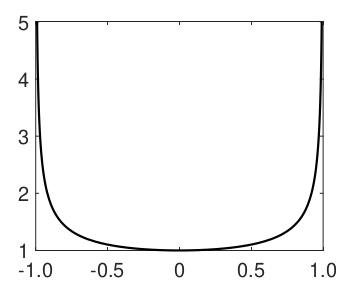
\includegraphics[width = 0.5\textwidth]{images/arcsin.png}
\end{center}

% \noindent{\bf 定义 4.59} 数量函数
% $$
% y = f(x)
% $$
% 的相对 (relative) 条件数 (condition number) 是
% $$
% C_f(x) = \left|\frac{x f'(x)}{f(x)}\right|.
% $$
% 从这个定义可以看到, 条件数考察的就是当输入 $x$ 有一个扰动成为 $x + \delta x$ 时,
% $y$ 的相对改变量:
% $$
% \hat{y} - y = f(x + \delta x) - f(x) = f'(x)\delta x + O(\delta x^2),
% $$
% 这里显然用了 Taylor 展开, 然后有
% $$
% \frac{\delta y}{y} = \left(\frac{x f'(x)}{f(x)}\right)\frac{\delta x}{x}
% + O(\delta x^2).
% $$

% \noindent{\bf 定义 4.60} 小条件数的问题我们称为是良态的 (well-conditioned),
% 大条件数的问题我们称为是病态的 (ill-conditioned).

% 注意条件数是数学问题决定的, 而不是算法决定的. 它是一个问题的计算上的困难的客观衡量.

\noindent \textbf{备注 4.43.} 定义 4.59 依赖于 $f(x) \neq 0$ 的条件。为了在函数 $f(x)$ 的根 $x = r$ 处定义条件数,我们转而使用绝对误差。

\noindent \textbf{引理 4.63.} 考虑在简单根 $r$ 附近求解方程 $f(x) = 0$, 即 $f(r) = 0$ 且 $f'(r) \neq 0$. 
假设我们扰动函数 $f$ 为 $F = f + \epsilon g$, 其中 $f, g \in \mathcal{C}^2$, 
$g(r) \neq 0$, 且 $|\epsilon g'(r)| \ll |f'(r)|$. 那么 $F$ 的根是 $r + h$, 其中
\[
  h \approx -\epsilon \frac{g(r)}{f'(r)}. \tag{4.32}
\]

\begin{proof}
假设 $r + h$ 是新根,即 $F(r + h) = 0$, 或者,
\[
  f(r + h) + \epsilon g(r + h) = 0.
\]

$F(r + h)$ 的泰勒展开式得出
\[
  f(r) + hf'(r) + \epsilon[g(r) + hg'(r)] = O(h^2)
\]
并且我们有
\[
  h \approx -\epsilon \frac{g(r)}{f'(r) + \epsilon g'(r)} \approx -\epsilon \frac{g(r)}{f'(r)}. 
\]
\end{proof}

\noindent \textbf{备注 4.44.} 对于引理 4.63 中的求根问题,我们不能基于相对误差定义条件数,
因为 $f(x) = 0$ 在 $x = r$ 处。然而,我们可以使用绝对误差定义条件数如下:
\[
  \left|\frac{r + h - r}{f(r) + \epsilon g(r) - f(r)}\right| = \left|\frac{1}{f'(r)}\right|,
\]
其中 $h$ 是输出的变化,而 $\epsilon g(r)$ 是输入的变化,分母用 Taylor 展开。上述方程意味着,如果 $|f'(r)|$ 接近零,
那么在 $r$ 处寻找 $f$ 的根的问题是非常病态的。(脑补一下什么场景?)

\noindent \textbf{例子 4.64 (Wilkinson).} 定义
\[
  f(x) := \prod_{k=1}^{p} (x - k),
\]
\[
  g(x) := x^p.
\]
根 $x = p$ 如何受到扰动 $f$ 到 $f + \epsilon g$ 的影响?根据引理 4.63,答案是
\[
  h \approx -\epsilon \frac{g(p)}{f'(p)} = -\epsilon \frac{p^p}{(p-1)!}.
\]
对于 $p = 20, 30, 40$, $\frac{p^p}{(p-1)!}$ 的值分别大约是 
$8.6 \times 10^8$, $2.3 \times 10^{13}$, $5.9 \times 10^{17}$. 
因此,单项式 $x^p$ 中系数的微小变化将导致根的大幅变化。
因此,对于非常高阶的多项式,求根问题是无望的。

% \noindent{\bf 引理 4.63} 对非线性方程
% $$
% f(x) = 0
% $$
% 在单根 $r$ 附近的求根. 也即 $f(r) = 0$, $f'(r) \neq 0$.
% 如果 $f$ (由于计算的原因) 受到扰动, 成为
% $$
% F = f + \epsilon g,
% $$
% 这里 $f, g \in C^2$, $g(r) \neq 0$, 且
% $$
% |\epsilon g'(r)| << |f'(r)|,
% $$
% 即导数上的扰动也是小量. 则 $F$ 有根 $r + h$, 其中
% $$
% h \approx \epsilon \frac{g(r)}{f'(r)}.
% $$
% 证明过程只需 Taylor 展开.

% 以上分析告诉我们, 从实数连续统到浮点运算系统, 从微积分到算法, 精确性和稳定性,
% 是普遍问题. 后者更加复杂且重要.

\subsubsection{向量函数的条件数}

\noindent \textbf{备注 4.45.} 定义 4.65 是定义 4.59 向量函数的直接和自然推广。

\noindent \textbf{定义 4.65.} 向量函数 $f : \mathbb{R}^m \rightarrow \mathbb{R}^n$ 的条件数是
\[
  \text{cond}_f(x) = \frac{\|x\| \|\nabla f\|}{\|f(x)\|}, \tag{4.33}
\]
其中 $\|\cdot\|$ 表示欧几里得范数,如 1-范数、2-范数和 $\infty$-范数。

\noindent \textbf{例子 4.66.} 在求解线性系统 $Au = b$ 时,算法可以被视为接受输入 $b$ 并返回输出 $A^{-1}b$, 
即 $f(b) = A^{-1}b$. 显然 $\nabla f = A^{-1}$. 定义 4.65 得出
\[
  \text{cond}_f(x) = \frac{\|b\| \|A^{-1}\|}{\|u\|} = \frac{\|Au\| \|A^{-1}\|}{\|u\|}.
\]
在实践中,输入 $b$ 可以取任何值,因此我们有
\[
  \max \text{cond}_f(x) = \max_{u \neq 0} \frac{\|Au\| \|A^{-1}\|}{\|u\|} = \|A\| \|A^{-1}\|,
\]
其中我们使用了常见的定义
\[
  \|A\| := \max_{u \neq 0} \frac{\|Au\|}{\|u\|}. \tag{4.34}
\]
这解释了定义 4.67。

\noindent \textbf{定义 4.67.} 非奇异方阵 $A$ 的条件数是
\[
\text{cond} A := \|A\| \|A^{-1}\|. \tag{4.35}
\]

\noindent \textbf{引理 4.68.} 基于 2-范数,非奇异方阵 $A$ 的条件数是
\[
\text{cond}_2 A := \|A\|_2 \|A^{-1}\|_2 = \frac{\sigma_{\text{max}}}{\sigma_{\text{min}}},
\]
其中 $\sigma_{\text{max}}$ 和 $\sigma_{\text{min}}$ 分别是 $A$ 的最大和最小奇异值。如果 $A$ 也是正规矩阵,我们有
\[
\text{cond}_2 A = \frac{|\lambda_{\text{max}}|}{|\lambda_{\text{min}}|},
\]
其中 $\lambda_{\text{max}}$ 和 $\lambda_{\text{min}}$ 分别是 $A$ 的最大和最小模的本征值。此外,如果 $A$ 是酉矩阵,我们有 $\text{cond}_2 A = 1$.

\noindent \textbf{例子 4.69.} 对于矩阵
\[
A = \begin{bmatrix}
1 & 1 - \delta \\
1 & 1 + \delta
\end{bmatrix}
\]
和 $\delta = 10^{-8}$,我们有 $\text{cond}_2 A = 19999999999.137258$.

\noindent \textbf{定理 4.70.} 设 $A$ 是一个可逆矩阵,$\hat{A}$ 是 $A$ 的一个扰动,满足
\[
\|A^{-1}\|\|\hat{A} - A\| < 1, \tag{4.37}
\]

设 \( \mathbf{x} \) 和 \( \hat{\mathbf{x}} \) 是线性系统的解
\[
A\mathbf{x} = \mathbf{b}, \quad \hat{A}\hat{\mathbf{x}} = \hat{\mathbf{b}}. \tag{4.38}
\]
那么 \( \hat{\mathbf{x}} \) 近似 \( \mathbf{x} \) 的相对误差有界为
\[
  \frac{\|\hat{\mathbf{x}} - \mathbf{x}\|}{\|\mathbf{x}\|} 
  \leq \frac{\text{cond} \, A}{1 - (\text{cond} \, A) \frac{\|\hat{A} - A\|}{\|A\|}} 
  \left( \frac{\|\hat{\mathbf{b}} - \mathbf{b}\|}{\|\mathbf{b}\|} + \frac{\|\hat{A} - A\|}{\|A\|} \right).\tag{4.39}
\]

\begin{proof}
写成 $\hat{A} = A[I + A^{-1}(\hat{A} - A)]$ 并且我们有从定理 E.76 和 (4.37) 得出 $\hat{A}$ 是可逆的,并且
\[
  \hat{A}^{-1} = [I + A^{-1}(\hat{A} - A)]^{-1}A^{-1}.
\]
然后定理 E.76 和三角不等式得出
\[
  \|A^{-1}|\leq \frac{\|A^{-1}\|}{1 - \|A^{-1}\|\|\hat{A} - A\|}.  \tag{4.40}
\]
%通过 (4.38) 我们可以写成 

根据(4.38),我们可以写出 
\[ 
  \hat{\mathbf{x}} - \mathbf{x} = \hat{A}^{-1}[\hat{\mathbf{b}} - \mathbf{b} - (\hat{A} - A)\mathbf{x}],
\]
结合(4.40)和三角不等式,得到
\[
  \frac{\|\hat{\mathbf{x}} - \mathbf{x}\|}{\|\mathbf{x}\|} \leq \frac{\text{cond} \, A}{1 - \|\hat{A} - A\|\|A^{-1}\|} 
  \left( \frac{\|\hat{\mathbf{b}} - \mathbf{b}\|}{\|A\|\|\mathbf{x}\|} + \frac{\|\hat{A} - A\|}{\|A\|} \right).
\]
然后(4.39)由 \( \|A\|\|\mathbf{x}\| \geq \|\mathbf{b}\| \) 得出。 
\end{proof}


这个定理告诉我们矩阵 $A$ 的扰动带来的影响。

\noindent \textbf{备注 4.46. } 线性系统的解在矩阵和右手边向量受到扰动时会发生变化。定理 4.70 量化了解的相对变化与矩阵条件数的关系。

\noindent \textbf{定义 4.71.} 向量函数 \( f: \mathbb{R}^m \to \mathbb{R}^n \) 的分量条件数为
\[
  \text{cond}_f(\mathbf{x}) = \|A(\mathbf{x})\|, \tag{4.41}
\]
其中矩阵 \( A(\mathbf{x}) = [a_{ij}(\mathbf{x})] \) 且每个分量为
\[
  a_{ij}(\mathbf{x}) = \left| \frac{x_j \frac{\partial f_i}{\partial x_j}}{f_i(\mathbf{x})} \right|. \tag{4.42}
\]

\noindent \textbf{备注 4.47.} 显然,(4.42) 来自于 (4.30)。但为什么我们首先需要定义 4.71 呢?
因为它可能比定义 4.65 更准确地描述算法的条件;毕竟,范数往往会抹去细节。

\noindent \textbf{例子 4.72.} 对于向量函数
\[
  f(\mathbf{x}) := \begin{bmatrix} \frac{1}{x_1} + \frac{1}{x_2} \\ \frac{1}{x_1} - \frac{1}{x_2} \end{bmatrix},
\]
其雅可比矩阵为
\[
  \nabla f = -\frac{1}{x_1^2 x_2^2} \begin{bmatrix} x_2^2 & x_1^2 \\ x_2^2 & -x_1^2 \end{bmatrix}.
\]
基于定义 4.71 的条件数清楚地捕捉到 \( x_1 \pm x_2 \approx 0 \) 导致条件不良的事实,其中
\[
  C_c = \|A_c\|,
\]
\[
  A_c = \begin{bmatrix} \left| \frac{x_2}{x_1 + x_2} \right| & \left| \frac{x_1}{x_1 + x_2} \right| \\ 
    \left| \frac{x_2}{x_1 - x_2} \right| & \left| \frac{x_1}{x_1 - x_2} \right| \end{bmatrix},
\]

基于定义 4.65 的 $1-$范数无法捕捉到条件不良的情况,
\[
  C_1 = \frac{\|\mathbf{x}\|_1 \|\nabla f\|_1}{\|f\|_1} = \frac{|x_1| + |x_2|}{|x_1 x_2|} \frac{2 \max(x_1^2, x_2^2)}{|x_1 + x_2| + |x_1 - x_2|},
\]

在条件 \( x_1 \pm x_2 \approx 0 \) 下,得到 \( C_1 \approx 2 \)。注意我们使用了著名的公式
\[
  \forall A \in \mathbb{R}^{n \times n}, \quad \|A\|_1 = \max_j \sum_i |a_{ij}|.
\]

\noindent \textbf{例子 4.73.} 如果参数 \( t_1, t_2, \ldots, t_n \) 在 \([-1, 1]\) 中等间距分布,
基于 \(\infty\)-范数的范德蒙矩阵的条件数在定义 2.3 中为

\[
\text{cond}_{\infty} V_n \sim \frac{1}{\pi} \exp \left[ -\frac{\pi}{4} + \frac{n}{4} (\pi + 2 \ln 2) \right],
\]

对于 \( n = 20 \),其值为 \( 9.86 \times 10^8 \).

\noindent \textbf{备注 4.48.} 我们知道从第二章中,多项式插值导致范德蒙矩阵,其大条件数是我们应该避免在等间距点上进行高阶多项式插值的另一个原因。
同样地,定义 4.74 中的希尔伯特矩阵自然地来自于函数的最佳多项式近似,这将在第五章中讨论,以 \( L_2 \) 范数为标准。

\noindent \textbf{定义 4.74.} 希尔伯特矩阵 \( H_n \in \mathbb{R}^{n \times n} \) 为
\[
h_{i,j} = \frac{1}{i + j - 1}.
\]

\noindent \textbf{例子 4.75.} 基于 2-范数的希尔伯特矩阵的条件数为
\[
  \text{cond}_2 H_n \sim \frac{(\sqrt{2} + 1)^{4n + 4}}{2^{15/4} \sqrt{\pi n}},
\]

对于 \( n = 10 \), 其值为 \( 9.22 \times 10^{14} \). 参见例子 5.42。

如果一个正问题会有巨大的向前误差,比如求多项式的值,比如求线性变换。
那么我们更加不能期待其反问题有良好的条件数,比如求根,比如线性方程组求解。
 
如果我们必须面对一个病态问题怎么办?这里如例 4.64 说 ``hopeless'' 有一点过于绝望了。 
如果我们数学上没有新的技巧来改进这个问题的条件数,那么有一个 ``万金油'' 方法是充分提升我们的浮点精度。
因此会有 GPM(GNU Multiple Precision Arithmetic Library) 这样的无限精度计算包。


% $$
% \hat{x} - x = \hat{A}^{-1}[\hat{b} - b - (\hat{A} - A)x],
% $$
% 这与 (4.40) 和三角不等式一起,得出
% \[
%   \frac{|\hat{x} - x|}{|x|} 
%   \leq \frac{\text{cond} A}{1 - (\text{cond} A)\frac{|\hat{A} - A|}{|A|}} \left(\frac{|\hat{b} - b|}{|b|} + \frac{|\hat{A} - A|}{|A|}\right).\tag{4.39}
% \]
% 然后 (4.39) 从 $|A||x| \geq |b|$ 得出。

% \noindent{\bf 定义 4.65} 向量函数
% $$
% \vec{f} : \mathbb{R}^m \to \mathbb{R}^n 
% $$
% 的条件数是
% $$
% \mbox{cond}_{\vec{f}}(\vec{x})
% = \frac{\|\vec{x}\|\|\nabla\vec{f}\|}{\|\vec{f}(\vec{x})\|},
% $$
% 这里范数可取 $p-$ 范数. 这个条件数基本是一元情形的自然推广.
% 它的一个重要特例是对线性方程组
% $$
% A \vec{x} = \vec{b}
% $$
% 有
% $$
% \vec{x} = A^{-1}\vec{b},
% $$
% 令 $\vec{f}(\vec{b}) = A^{-1}\vec{b}$, 则 $\nabla \vec{f} = A^{-1}$.
% 于是 $f$ 的条件数为:
% $$
% \mbox{cond}_{\vec{f}}(\vec{b})
% = \frac{\|\vec{b}\|\|A^{-1}\|}{\|\vec{x}\|}
% = \frac{\|A\vec{x}\|\|A^{-1}\|}{\|\vec{x}\|}.
% $$
% 如果我们把向量范数和矩阵范数用诱导公式
% $$
% \|A\| = \max_{\vec{u} \neq 0}\frac{\|A\vec{u}\|}{\|\vec{u}\|}
% $$
% 联系起来, 那么就有
% $$
% \mbox{cond}_A := \|A\|\|A^{-1}\|.
% $$
% 这是判断矩阵问题是否病态的重要指标. 例 4.69 给出了一个病态矩阵的例子. 注意到, 
% 对问题 $A x = b$, 有
% $$
% \left[
% \begin{array}{cc}
%   1 & 1 - \delta \\
%   1 & 1 + \delta
% \end{array}
% \right]\left[\begin{array}{c}
%   x_1 \\ x_2
% \end{array}
% \right] = \left[\begin{array}{c}
%   b_1 \\ b_2
% \end{array} \right] \Rightarrow x_2 = \frac{b_2 - b_1}{2 \delta}.
% $$
% 于是 $b_2 - b_1$ 的舍入误差 $\epsilon_u$ 会被放大到 $\frac{1}{\delta}$. 
% 导致这个线性方程组数值求解困难. 定理 4.70 将这个问题推广到一般. 


% \noindent{\bf 定义 4.71} 向量函数 $\vec{f}: \mathbb{R}^m \to \mathbb{R}^n$
% 分量形式的条件数为:
% $$
% \mbox{cond}_{\vec{f}}(\vec{x}) = \|A(\vec{x})\|,
% $$
% 其中 $A(\vec{x}) = [a_{ij}(\vec{x})]$ 为
% $$
% a_{ij}(\vec{x})
% = \left|\frac{x_j\frac{\partial f_i}{\partial x_j}}{f_i(\vec{x})}\right|.
% $$
% 这个分量形式的结果, 有时会比向量形式(定义 4.65) 更加精确一些, 例 4.67 给出了一个定义4.71 
% 比定义 4.65 更好捕捉到病态性质的例子. 注意条件数一般用于理论分析, 
% 不用于计算的判定. 也就是作为一个算法, 并不会去算条件数. 只有在分析这个算法是否病态时, 
% 才会从理论角度去分析.

% 定义 4.73 说明了 Vandermonde
% 矩阵也是病态的. 对于病态的矩阵, 唯一的办法是绕路走. 
% 这也是为什么第二章我们不能直接求解这个矩阵的原因之一.

\subsubsection{算法的条件数}

问题的条件数不好,说明要么这个问题建模有错,要么这个问题本质上就是不稳定的。比如物理上,这就是一个混沌问题。
比如台风路径的预测。有时候一点小扰动,比如一只乌鸦飞过,就会导致完全不同的结果。

更多的时候,我们面对的问题并没有这么病态,这个时候,我们要小心不好的算法带来额外的困难。如果说问题条件数,
衡量的是探索自然界的艰难,那么算法条件数,某种程度上是在衡量我们的人类的愚蠢。

\noindent \textbf{备注 4.49. } 第 4.3.3 节和 4.3.4 节中的条件数衡量了数学问题对输入变化的敏感性,
而定义 4.76 衡量了一个算法的稳健性。如果数学问题的条件数足够大,那么对该问题的任何数值计算都是无望的。
相比之下,对于一个不稳定的算法,可能存在另一个算法以稳定的方式计算相同的基础问题,参见例子 4.51。

\noindent \textbf{定义 4.76. } 考虑用算法 \( f_A : \mathcal{F}^m \rightarrow \mathcal{F}^n \) 来近似一个函数 \( f : \mathbb{R}^m \rightarrow \mathbb{R}^n \).
假设
\[
  \forall \mathbf{x} \in \mathcal{F}^m, \, \exists \mathbf{x}_A \in \mathbb{R}^m \text{ 使得 } f_A(\mathbf{x}) = f(\mathbf{x}_A),
\]

算法 \( f_A \) 的条件数由下式给出
\[
  \text{cond}_A(\mathbf{x}) = \frac{1}{\epsilon_u} \inf_{\{\mathbf{x}_A\}} \frac{\|\mathbf{x}_A - \mathbf{x}\|}{\|\mathbf{x}\|},
\]

其中 \( \epsilon_u \) 是定义4.26中 \( \mathcal{F} \) 的单位舍入误差。如果算法 \( f_A \) 的条件数接近 $1$, 则算法是条件良好的;否则,算法是条件不良的。

这里 ``接近 $1$'' 的实际含义是一个不要太大的有界量。这个定义的实际含义是:你计算的是 $x$, 但在问题眼里,你计算的是 $x_A$.
所以产生的绝对误差相比当前的机器精度是多少?

\noindent \textbf{备注 4.50.} 函数 \( f: \mathbb{R}^m \rightarrow \mathbb{R}^n \) 下的 \( y \in \mathbb{R}^n \) 的纤维是集合
\[
f^{-1}(y) = \{ \mathbf{x} : f(\mathbf{x}) = y \}.
\]

因此,定义4.76中的条件数可以被视为 \( f^{-1} \) 在 \( y \) 处的精度度量,相对于(4.45)中取的下确界。因此,根据定义,精度和稳定性在某种程度上有重叠。

\noindent \textbf{例子 4.77.} 考虑一个用于计算 \( y = \ln x \) 的算法 \( A \). 
假设对于任何正数 \( x \), 该程序产生一个 \( y_A \) 满足 \( y_A = (1 + \delta) \ln x \) 其中 \( |\delta| \leq 5 \epsilon_u \). 
算法的条件数是多少?我们显然有
\[
  y_A = \ln x_A \text{ 其中 } x_A = x^{1 + \delta},
\]
因此
\[
  E_{\text{rel}}(x_A) = \left| \frac{x^{1 + \delta} - x}{x} \right| = |x^\delta - 1| = |e^{\delta \ln x} - 1|
\]
\[
\approx |\delta \ln x| \leq 5 |\ln x| \epsilon_u.
\]
因此,除非 \( x \rightarrow 0^+ \),否则 \( A \) 是条件良好的。


\noindent \textbf{备注 4.51.} 显然,(4.45) 意味着

\[
  \forall \mathbf{x}_A \text{ 满足 } (4.44), \, \text{cond}_A(\mathbf{x}) \leq \frac{1}{\epsilon_u} \frac{\|\mathbf{x}_A - \mathbf{x}\|}{\|\mathbf{x}\|}.
\]
根据定义4.52和4.76,算法 \( A \) 的条件数 \( \text{cond}_A(\mathbf{x}) \) 很小等价于 \( A \) 是向后稳定的。

估计算法条件数的一种方法是将其与数学问题的条件数联系起来。

\noindent \textbf{定理 4.78. } 假设一个光滑函数 \( f: \mathbb{R} \rightarrow \mathbb{R} \) 
被一个算法 \( A: \mathcal{F} \rightarrow \mathcal{F} \) 近似,产生 \( f_A(x) = f(x)(1 + \delta(x)) \) 其中 
\( |\delta(x)| \leq \varphi(x) \epsilon_u \). 如果 \( \text{cond}_f(x) \) 是有界且非零的,那么我们有
\[
  \forall x \in \mathcal{F}, \quad \text{cond}_A(x) \leq \frac{\varphi(x)}{\text{cond}_f(x)}. \tag{4.46}
\]

注意这里,问题条件数是客观的,我们不能去改。而且这里指出,问题条件数是良好的,有界,不为零。
这里 $\varphi(x)$ 是 $\delta(x)$ 去掉精度量纲的上界.  这个定理建立问题条件数和算法条件数之间的关系。

\begin{proof}
假设 \( \forall x, \, \exists x_A \) 使得 \( f(x_A) = f_A(x) \). 写成 \( x_A = x(1 + \epsilon_A) \) 并且我们有
\[
  f(x)(1 + \delta) = f(x_A) = f(x(1 + \epsilon_A)) = f(x + x \epsilon_A)
\]
\[
  = f(x) + x \epsilon_A f'(x) + O(\epsilon_A^2).
\]
  
忽略二次项得到
\[
  x \epsilon_A f'(x) = f(x) \delta
\]
\[
  \Rightarrow \left| \frac{x_A - x}{x} \right| = |\epsilon_A| = \left| \frac{f(x)}{x f'(x)} \right| |\delta(x)|.
\]
  
两边同时除以 \( \epsilon_u \) 得到
\[
  \frac{1}{\epsilon_u} \left| \frac{x_A - x}{x} \right| = \frac{\delta(x)}{\epsilon_u \text{cond}_f(x)}.
\]
对所有 \( x_A \) 取下确界,应用条件 \( |\delta(x)| \leq \varphi(x) \epsilon_u \),我们得到(4.46)。 
\end{proof}

\noindent \textbf{备注 4.52.} (4.46)中的不等式仅来自于条件 \( |\delta| \leq \varphi(x) \epsilon_u \),
其中 \( \varphi(x) \) 作为上界,代表了最坏情况下的场景。因此,(4.46)中的 RHS 应该被解释为给定 \( x \) 的最大条件数的估计。
这是一个 ``最大-最小'' 特征,其中最小值是在所有满足 \( f_A(\mathbf{x}) = f(\mathbf{x}_A) \) 的 \( \mathbf{x}_A \) 上取的,
最大值是在算法的所有可能输入上取的。

\noindent \textbf{例子 4.79.} 假设 \( \sin x \) 和 \( \cos x \) 是在机器精度内以相对误差计算的(这可以通过截断泰勒级数轻松满足)。
应用定理4.78来分析算法的条件数
\[
  f_A = \text{fl} \left[ \frac{\text{fl}(1 - \text{fl}(\cos x))}{\text{fl}(\sin x)} \right]
\]

对于 \( x \in (0, \pi/2) \) 计算 \( f(x) = \frac{1 - \cos x}{\sin x} \)。根据定义4.59,很容易计算出
\[
  \text{cond}_f(x) = \frac{x}{\sin x}.
\]

此外,根据定理4.40和对 \( \sin x \) 和 \( \cos x \) 的假设,我们有

\[
  f_A(x) = \frac{(1 - (\cos x)(1 + \delta_1))(1 + \delta_2)}{(\sin x)(1 + \delta_3)}(1 + \delta_4),
\]

其中 \( |\delta_i| \leq \epsilon_u \) 对于 \( i = 1, 2, 3, 4 \)。忽略二次项 \( O(\delta_i^2) \),上述方程等价于

\[
  f_A(x) = \frac{1 - \cos x}{\sin x} \left\{ 1 + \delta_2 + \delta_4 - \delta_3 - \delta_1 \frac{\cos x}{1 - \cos x} \right\},
\]

因此我们有 \( \varphi(x) = 3 + \frac{\cos x}{1 - \cos x} \) (每一个 $\delta_i$ 都看成 $\epsilon_u$)并且

\[
  \text{cond}_A(x) \leq \frac{\sin x}{x} \left( 3 + \frac{\cos x}{1 - \cos x} \right).
\]

因此,当 \( x \rightarrow 0 \) 时,\( \text{cond}_A(x) \) 可能是无界的。
另一方面,当 \( x \rightarrow \frac{\pi}{2} \) 时,\( \text{cond}_A(x) \) 由 \( \frac{6}{\pi} \) 控制。

\noindent \textbf{备注 4.53.} 在例子4.79中,当 \( x \rightarrow 0 \) 时,数学问题的条件数为 $1$,
而算法(4.47)的条件数为无穷大。
这是一个典型的例子,说明一个不小心的实现可能会改变数学问题的条件性质。为了恢复数学问题在 \( x \rightarrow 0 \) 时的良好条件,
应该通过泰勒级数重写 \( f \) 以获得另一个算法。

\noindent \textbf{练习 4.80.} 在相同的区间上重复例子4.79,对于 \( f(x) = \frac{\sin x}{1 + \cos x} \).

\noindent \textbf{备注 4.54.} 我们已经量化了数学问题和相应算法的敏感性。当我们使用算法来解决数学问题时,问题的条件数和算法的条件数都影响整体误差。

\subsubsection{机器求解的整体误差}
% 4.3.6

\begin{center}
  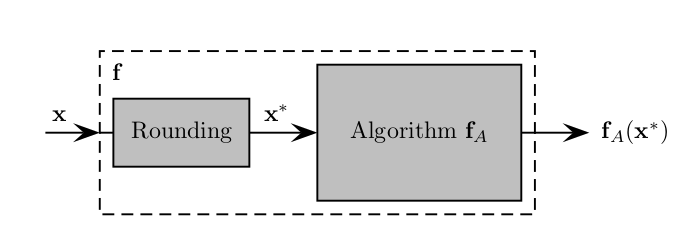
\includegraphics[width = 0.7\textwidth]{images/error.png}
\end{center}

\noindent \textbf{定理 4.81.} 如图4.4所示,考虑使用标准化的浮点数算术来解决数学问题
\[
f: \mathbb{R}^m \rightarrow \mathbb{R}^n, \quad \mathbf{y} = f(\mathbf{x}).
\]

将计算机的输入和输出表示为
\[
\mathbf{x}^* \approx \mathbf{x}, \quad \mathbf{y}_A^* = f_A(\mathbf{x}^*),
\]
其中 \( f_A \) 是近似 \( f \) 的算法。用 \( \mathbf{y}_A^* \) 近似 \( \mathbf{y} \) 的相对误差可以限定为
\[
  E_{\text{rel}}(\mathbf{y}_A^*) \lessapprox E_{\text{rel}}(\mathbf{x}^*) \text{cond}_f(\mathbf{x}) + \epsilon_u \text{cond}_f(\mathbf{x}^*) \text{cond}_A(\mathbf{x}^*),
\]
其中相对误差在(4.25)中定义。

\begin{proof}
根据三角不等式,我们有
\[
  \frac{\|\mathbf{y}_A^* - \mathbf{y}\|}{\|\mathbf{y}\|} = \frac{\|f_A(\mathbf{x}^*) - f(\mathbf{x})\|}{\|f(\mathbf{x})\|}
\]
\[
  \leq \frac{\|f(\mathbf{x}^*) - f(\mathbf{x})\|}{\|f(\mathbf{x})\|} + \frac{\|f_A(\mathbf{x}^*) - f(\mathbf{x}^*)\|}{\|f(\mathbf{x})\|}.
\]
根据(4.31),第一项是
\[
  \frac{\|f(\mathbf{x}^*) - f(\mathbf{x})\|}{\|f(\mathbf{x})\|} \lessapprox \text{cond}_f(\mathbf{x}) \frac{\|\mathbf{x}^* - \mathbf{x}\|}{\|\mathbf{x}\|}
\]
\[
  = E_{\text{rel}}(\mathbf{x}^*) \text{cond}_f(\mathbf{x}).
\]
根据(4.31)和定义4.76,第二项是
\[
  \frac{\|f_A(\mathbf{x}^*) - f(\mathbf{x}^*)\|}{\|f(\mathbf{x})\|} = \frac{\|f(\mathbf{x}_A^*) - f(\mathbf{x}^*)\|}{\|f(\mathbf{x})\|} \approx \frac{\|f(\mathbf{x}_A^*) - f(\mathbf{x}^*)\|}{\|\mathbf{x}^*\|}
\]
\[
  \leq \text{cond}(\mathbf{x}^*) \frac{\|\mathbf{x}_A^* - \mathbf{x}^*\|}{\|\mathbf{x}^*\|}
\]
\[
  = \epsilon_u \text{cond}_A(\mathbf{x}^*) \text{cond}_f(\mathbf{x}^*),
\]
其中最后一步遵循于我们只考虑最不危险的 \( \mathbf{x}_A^* \).
\end{proof}

\noindent \textbf{备注 4.55.} 根据定理4.81,希望近似一个条件数过大的函数是没有希望的:(4.50)的右侧每个求和项都包含一个因子 
\( \text{cond}_f(\mathbf{x}^*) \) 或 \( \text{cond}(\mathbf{x}) \)。另一方面,对于条件良好的函数,设计一个近似算法时仍需小心,
因为术语 \( \text{cond}_A(\mathbf{x}^*) \) 可能会使(4.50)的右侧界限过大。

\noindent \textbf{备注 4.56.} 关于计算机算术与数值精度和稳定性之间相互作用的更多例子,请参阅Higham 2002年出版的书籍。 

% \noindent{\bf 定义 4.76} 考虑在浮点系统 $\mathscr{F}$ 下近似计算向量函数,
% 即用
% $$
% \vec{f}_A : \mathscr{F}^m \to \mathscr{F}^n
% $$
% 来近似计算
% $$
% \vec{f} : \mathbb{R}^m \to \mathbb{R}^n.
% $$
% 如果
% $$
% \forall \vec{x} \in \mathscr{F}^m, \exists \vec{x}_A \in \mathbb{R}^m,
% $$
% 使得
% $$
% \vec{f}_A(\vec{x}) = \vec{f}(\vec{x}_A),
% $$
% 那么 $\vec{f}_A$ 的条件数是
% $$
% \mbox{cond}_A (\vec{x}) = \frac{1}{\epsilon_u}
% \inf_{\{\vec{x}_A\}}\frac{\|\vec{x}_A - \vec{x}\|}{\|\vec{x}\|}.
% $$
% 也即由舍入误差可能引起的最大干扰. 而定理 4.78 给出了条件数的上界.

% \begin{remark}

%   函数 $f : \mathbb{R}^m \rightarrow \mathbb{R}^n$ 下的 $y \in \mathbb{R}^n$ 的纤维是集合
% \[f^{-1}(y) = \{x : f(x) = y\}\]
% 因此, 定义4.76中的条件数可以被视为度量 $f^{-1}$ 在 $y$ 处对于 (4.45) 中所取的下确界的准确性. 
% 因此, 按定义精确性和稳定性具有一定程度的重叠.

% (4.46)中的不等式仅来自于条件 $|\delta| \leq \phi(x)\epsilon_u$,
% 其中$\phi(x)$作为一个上界, 表示最坏情况的情景. 因此, (4.46)中的RHS应该被解释为给定$x$的条件数的最大估计. 
% 这是一个``最大-最小''特性, 其中最小值取自所有满足 (4.44) 中的 $f_A(x) = f(x_A)$ 的 $x_A$, 
% 而最大值则取自算法的所有可能输入. 

% 在例 4.79 中, 当 $x \rightarrow 0$ 时, 数学问题的条件数为 $0$, 
% 因为 
% $$
% \lim_{x\rightarrow0} \frac{x^2}{2\sin x} = 0,
% $$
% 而算法 (4.47) 的条件数为 $\infty$. 这是一个典型的示例, 表明粗心的实现可能改变数学问题的条件属性. 
% 为了在 $x \rightarrow 0$ 的情况下恢复数学问题的良好条件, 应通过 Taylor 级数重写 $f$, 以得到另一种算法.
% \end{remark}

% \noindent \textbf{备注 4.54.} 我们已经量化了数学问题和相应算法的敏感性。当我们使用算法来解决数学问题时,问题的条件数和算法的条件数都影响整体误差。

% 我们已经量化了数学问题以及相应算法的敏感性. 当我们使用算法来解决数学问题时, 
% 问题的条件数和算法的条件数都会影响总体误差. 

% 作为一整章的总结, 最后的定理 4.81 表达的意思是: 如果函数$f$的条件数过大, 那么近似它是不可行的: 
% (4.50)在右侧的每一项中都包含一个因子$condf(x^*)$或$condf(x)$. 另一方面, 
% 对于一个条件良好的函数$f$, 在设计近似算法时仍需要谨慎, 否则$condA(x^*)$这一项可能会使(4.50)右边的上界过大.

% 关于计算机算术与数值精度和稳定性之间的交互的更多例子, 读者可以参考Higham [2002]的书.


\section*{计算软件介绍}

eigen

我们已经学习了一些基本的计算方法, 以及浮点数计算原理. 这一周我们水一下.
主要目的是给大家完成项目作业创造契机.

正如前面所说, 在可见的未来, 我们几乎不会直接在实际工作中使用我们自己编写的程序,
因为不可靠. 一般来说, 我们在从事实际工作时, 会处于两种境界:

\begin{enumerate}
\item 使用某个现成的集成平台, 比如 Matlab;
\item 使用 C++ 构建一个触及前沿的算法, 但是依赖各种成熟的软件库.
\end{enumerate}

我们下面分别就这两种境界做一些简单的介绍.

\subsection*{集成平台}
目前实际可用的跨操作系统的平台, 主要有两个: Matlab 和 Python. 前者是一个成熟的商业软件,
大家可以从我们学校获得正版序列号. 但由于大家都知道的原因, 我已经停用很久了. Python 严格来说,
只是提供了一种语言生态, Python 语言因为向上短平快, 向下对接高效率二进制库,
所以成为各种库的超级市场, 其中也有完善的科学计算支持. 它的最大优点是非常容易学习和使用.
相信今天晚上大家都能成为 Python 科学计算专家.

这里顺便说一句, 目前我们国家有一批应用数学家, 推出了一款叫做``北太天元''的软件,
主要任务是在脚本级别替代 Matlab, 也就是说, Matlab 的 .m 文件, 在它上面可以正常运行并得到正确结果.
大家可以关注一下.

\subsubsection*{Anaconda}
首先介绍一下 Python 的科学计算集成环境. 这个我在暑期课程数学软件中已经介绍过. 我个人推荐
Anaconda, 大家可以到清华的 tuna 站获取. 记得需要把源站点替换为 tuna,
这样在日后更新或构建新环境就可以提高速度.

大家在安装的时候也可以只安装 Minicoda, 然后用 conda 来维护.

在安装完成之后, 我们的 shell 会出现一个 base 前缀, 这个是 conda 的环境, 如果不想要这个,
可以在 .bashrc 文件中注释掉这一行. 在终端下输入:
\begin{verbatim}
env | grep CONDA
\end{verbatim}
可以看到具体环境变量的修改.

个人建议: 我们永远也不要去修改 base 环境, 将它作为基础, 重新构建我们要做具体工作的环境.
比如我总是用 teaching 环境来处理和教学有关的工作.

Anaconda 是第三方公司提供的集成科学计算环境, 严格来说, 它也不是完全开源和安全的.

在这个环境中, 对我们计算数学初级阶段学习比较有用的包如下:

\begin{enumerate}
\item jupyter-notebook, 代码和 markdown 文档混合的笔记本;
\item matplotlib, 科学绘图;
\item numpy, 向量和矩阵基础计算;
\item scipy, 数值计算的基本算法;
\item sympy, 符号计算的基本算法;
\end{enumerate}

以上包再配合上 Python 的一些基本功能, 能完成本科阶段的大部分学习需求.
这里接下去我们就直接使用 Jupyter Notebook 介绍. Markdown 是一种轻量级的笔记格式,
支持简单的格式化和 Latex, 但后者依赖具体的软件. 

在 Anaconda 中, Jupyter Notebook 其实是通过一个后台的 httpd 服务提供输出的,
因此我们可以在浏览器中直接使用.

以下进入 Jupyter-Notebook.

\section{最佳逼近和最小二乘}
% 5

\noindent {\bf 定义 5.1} 给定一个函数的赋范向量空间 \( Y \) 及其子空间 \( X \subset Y \). 如果函数 \( \hat{\varphi} \in X \) 满足
\[
  \forall \varphi \in X, \quad \|f - \hat{\varphi}\| \leq \|f - \varphi\|. \tag{5.1}
\]
则称 \( \hat{\varphi} \) 为 \( f \in Y \) 从 \( X \) 出发关于范数 \( \|\cdot\| \) 的最佳逼近。

\noindent \textbf{备注 5.1} 需要注意的是,定义 5.1 中的 \( \hat{\varphi} \) 也可以被视为一个优化问题的解,
\[
  \hat{\varphi} = \arg\min_{\varphi \in X} \|\varphi - f\|,
\]
其中 \( f \in Y \) 且 \( X \subset Y \).

\noindent \textbf{例子 5.2} 切比雪夫定理 2.47 可以按照定义 5.1 的格式重新表述如下。
如同例子 B.25 中,用 \( P_{n}(\mathbb{R}) \) 表示所有系数在实数域 \( \mathbb{R} \) 中且次数不超过 \( n \) 的多项式的集合。
对于 \( Y = P_{n}(\mathbb{R}) \) 和 \( X = P_{n-1}(\mathbb{R}) \), \( f(x) = -x^n \) 在 \( Y \) 中从 \( X \) 
出发关于最大范数 \( \|\cdot\|_{\infty} \) 的最佳逼近
\[
  \|g\|_{\infty} = \max_{x \in [-1,1]} |g(x)| \tag{5.2}
\]
是 \( \hat{\varphi} = \frac{T_{n}}{2^{n-1}} - x^n \),其中 \( T_{n} \) 是次数为 \( n \) 的切比雪夫多项式。显然,\( \hat{\varphi} \) 满足 (5.1).

\hl{例 5.2}  Chebyshev 定理 2.46 说, 记 $\tilde{{\mathbb{P}}}_n$, 为全部 $n$ 次且首项系数为 $1$ 
的多项式空间, $n \in \mathbb{N}^+$, 则
$$
\forall p_n(x) \in \tilde{\mathbb{P}_n}, 
\max_{x \in [-1, 1]}\left|\frac{T_n(x)}{2^{n - 1}}\right|
\leq \max_{x \in [-1, 1]} |p_n(x)|.
$$
现在我们取 $f(x) = -x^n \in Y = \mathbb{P}_n$, 这里 $\mathbb{P}_n$ 是最高次到 $n$ 的多项式空间.
而取 $X = \mathbb{P}_{n - 1}$, 则 $X$ 中关于 $f$ 的基于无穷范数的最佳逼近元为 
(不妨设定义域仍为 $[-1, 1]$):
$$
\hat{\phi}(x) = \frac{T_n(x)}{2^{n - 1}} - x^n.
$$
显然, $\forall \phi(x) \in X$, $\phi(x) - f(x) \in \tilde{\mathbb{P}}_{n}$ 是首项为 $1$ 的
$n$ 次多项式, 因此由 Chebyshev 定理 2.46, 误差在无穷范数 (又称最大模范数)
$$
\|g(x)\|_\infty := \max_{x \in [-1, 1]}|g(x)|
$$
下最小就是
$$
\|\phi(x) - f(x)\|_\infty \leq \|\hat{\phi}(x) - f(x)\|_\infty 
= \|\frac{T_n(x)}{2^{n - 1}} - x^n + x^n\|_\infty = \|\frac{T_n(x)}{2^{n - 1}}\|_\infty.
$$

\subsection{线性逼近的基本问题}

\hl{定义 5.3} 线性最佳逼近基本问题 (the fundamental problem of linear approximation), 
对 $f \in Y$, 求最佳逼近元
$$
\hat{\phi}(x) = \sum_{i = 1}^n u_i(x), 
$$
这里
$$
X = \mbox{span}\{u_1, u_2, \cdots, u_n\} \subset Y
$$
已知.

\hl{例 5.4} 对 $f(x) = e^x \in Y = C^\infty[-1, 1]$, 
求最佳逼近元
$$
\hat{\phi}(x) = \sum_{i = 1}^n x^i, 
$$
这里
$$
X = \mbox{span}\{1, x, x^2, \cdots, x^n\} \subset Y.
$$
在具体选取的范数上, 不同的范数代表了不同的空间, 不同的逼近方式和不同的算法策略.
比如可以取无穷范数, $1$-范数:
$$
\|g(x)\| := \int_a^b |g(x)| dx,
$$
或 $2$-范数:
$$
\|g(x)\|_2 := \left(\int_a^b g^2(x) dx\right)^\frac{1}{2}.
$$

回顾:

\hl{定义 3.71} (累积弦长, the cumulative chordal length) 空间 $\mathbb{R}^D$ 中 $n$
个点列 $\{x_1, x_2, \cdots, x_n\}$ 的累积弦长是指  
$$
t_i = \left\{
\begin{array}{ll}
  0, i = 1\\
  t_{i - 1} + \|x_i - x_{i - 1}\|_2.
\end{array}
\right.
$$

\hl{例 5.5} 对二维简单封闭曲线(只有一个圈) $\gamma : [0, 1) \to \mathbb{R}^2$ 
上的 $n$ 个点 $\vec{x}_i$, $i = 1, 2, \cdots, n$. 我们用它的累积弦长, 并缩放到 $[0, 1)$ 做参数,
用 $\vec{x}_i$, $i = 1, 2. \cdots, n$ 产生样条 $p$. 然后我们定义从 $0$ 出发, 沿参数化曲线 $\gamma$ 前进, 
左侧的面积记为 $\mbox{Int}(\gamma)$, 那么 $\mathcal{S}_1 = \mbox{Int}(\gamma)$ 和 
$\mathcal{S}_2 = \mbox{Int}(p)$ 的区别可定义为: 
$$
\|\mathcal{S}_1 - \mathcal{S}_2\|_1 := \int_{\mathcal{S}_1 \oplus \mathcal{S}_2} d\vec{x},
$$
这里 
$$
\mathcal{S}_1 \oplus \mathcal{S}_2 := \mathcal{S}_1 \cup \mathcal{S}_2 \backslash (\mathcal{S}_1 \cap \mathcal{S}_2).
$$
可以看作是两条曲线本质区别的量化. 所以我们可以基于 $1$-范数给出一个关于样条拟合的最佳逼近问题.

\hl{定理 5.6} 假设 \( X \) 是赋范向量空间 \( (Y, \|\cdot\|) \) 的有限维子空间。那么我们有
\[
  \forall y \in Y, \exists \hat{\varphi} \in X \text{ 使得 } \forall \varphi \in X, \|\hat{\varphi} - y\| \leq \|\varphi - y\|. \tag{5.5}
\]

\begin{proof}
对于给定的 \( y \in Y \), 定义一个闭球
\[
  B_{y} := \{x \in X : \|x\| \leq 2\|y\|\}.
\]
显然 \( 0 \in B_{y} \), 并且 \( y \) 到 \( B_{y} \) 的距离是
\[
  \operatorname{dist}(y, B_{y}) := \inf_{x \in B_{y}} \|y - x\| \leq \|y - 0\| = \|y\|.
\]
  
根据定义,任何 \( z \in X, z \notin B_{y} \) 必须满足 \( \|z\| > 2\|y\| \),因此
\[
  \|z - y\| \geq \|z\| - \|y\| > \|y\|.
\]
  
因此,如果存在对 \( y \) 的最佳逼近,它必须在 \( B_{y} \) 中。作为 \( X \) 的子空间,\( B_{y} \) 是有限维的、闭的、有界的,
因此 \( B_{y} \) 是紧致的。极值定理指出,连续标量函数在紧致集上取得其最小值和最大值。
范数是一个连续函数,因此函数 \( d: B_{y} \rightarrow \mathbb{R}^{+} \cup \{0\} \) 由 \( d(x) = \|x - y\| \) 给出,
必须在 \( B_{y} \) 上取得其最小值。
\end{proof}

\noindent \textbf{备注 5.2} 更一般地,连续函数保持包括紧致性在内的拓扑性质。对于连续函数 \( f: X \rightarrow \mathbb{R} \), 
在 \( X \) 的紧致子集上取得最小值和最大值是由 \( f \) 的像的紧致性保证的。

\noindent \textbf{备注 5.3} 最佳逼近的唯一性超出了本书的范围,可以在许多泛函分析教科书中找到。

\noindent \textbf{定理 5.7} 连续函数集 \( \mathcal{C}[a, b] \) 在 \( [a, b] \) 上是复数域 \( \mathbb{C} \) 上的内积空间,其内积定义为
\[
  \langle u, v \rangle := \int_a^b \rho(t) u(t) \overline{v(t)} \, dt, \tag{5.6}
\]
其中 \( \overline{v(t)} \) 是 \( v(t) \) 的复共轭,权重函数 \( \rho(x) \in \mathcal{L}[a, b] \) 满足对所有 \( x \in (a, b) \) 有 \( \rho(x) > 0 \). 
此外,\( \mathcal{C}[a, b] \) 与
\[
  \|u\|_2 := \left( \int_a^b \rho(t) |u(t)|^2 \, dt \right)^{\frac{1}{2}} \tag{5.7}
\]
是复数域 \( \mathbb{C} \) 上的赋范向量空间。

\begin{proof}
这遵循定义 B.2、B.165 和 B.170。
\end{proof}

\noindent \textbf{备注 5.4} \( |u(t)|^2 \) 可能与 \( u^2(t) \) 不同,因为底层域可能是复数!

\noindent \textbf{定义 5.8} \( \mathcal{C}[a, b] \) 上的最小二乘逼近是一个最佳逼近问题,其范数在 (5.1) 中设置为 (5.7) 中的范数。

\noindent \textbf{备注 5.5} 最小二乘逼近是我们在本章中关注的一种特殊类型的最佳逼近。此后,没有下标的范数意味着 2-范数。
请注意,基于其他范数(如 1-范数和最大范数)的最佳逼近问题的解决方案需要完全不同的工具,这是由于这些范数的不同性质;参见 Powell[1981]。

% \hl{定理 5.6} 若 $X$ 是赋范向量空间 $Y$ 的有限维线性空间, 则 $\forall y \in Y$, $X$ 中的最佳逼近元存在, 也即
% $$
% \exists \hat{\phi} \in X, s.t. \forall \phi \in X, \|\hat{\phi} - y\| \leq \|\phi - y\|. 
% $$

% 该定理的证明使用了极值原理 (the extreme value theorem, 闭区间上连续函数必有最大最小值, 扩展到一般赋范空间就是紧集上的连续函数必能取到极值. )
% 首先对 $\forall y \in Y$, 弄个圆框住它 (有界闭集):
% $$
% B_y := \{x \in X, \|x\| > 2\|y\|\}.
% $$
% 然后最佳逼近元一定不可能在圆外, 因为圆内至少有一个零元和 $y$ 的距离是 $\|y\|$. 然后在圆内, $\|x - y\|$ 是一个连续函数. 搞定.
% (紧性是随连续映射传递的.)

% 这本书不讨论最佳逼近元的唯一性, 自己看泛函分析的书.

% \hl{定理 5.7} 从 $[a, b] \to \mathbb{C}$ 的连续映射关于内积
% $$
% <u, v> := \int_a^b \rho(t) u(t) \bar{v(t)} dt
% $$
% 构成内积空间. 这里 $\rho(t) > 0$ 是实值的权重函数, $\bar{v(t)}$ 表示 $v(t)$ 的共轭. 注意由该内积可自然诱导 $2$-范数:
% $$
% \|u\|_2 := \left(\int_a^b |u(t)|^2\right)^\frac{1}{2},
% $$
% 这里 $|u(t)|$ 表示 $u(t)$ 的模. 注意此时, $u^2(t)$ 和 $|u(t)|^2$ 是不同的.

% \hl{定义 5.8} (最佳平方逼近, the least-square approximation), 即逼近范数采用 $2$-范数的最佳逼近.

% 由于最佳平方逼近的重要性, 我们本章将主要集中于这个问题. 本章剩下的部分, 默认范数为 $2$-范数.

\subsection{正交系统}
% 5.2

\hl{定义 5.9} 内积空间 \( X \) 的子集 \( S \) 是正交的,当且仅当
\[
\forall u, v \in S, \quad \langle u, v \rangle = \begin{cases} 
0 & \text{如果 } u \neq v, \\
> 0 & \text{如果 } u = v.
\end{cases} \tag{5.8}
\]

\hl{定理 5.10} 任何有限的非零正交元素集合 \( u_1, u_2, \ldots, u_n \) 是线性无关的。

\begin{proof}
这是通过使用定义 B.26 和 5.9 进行反证法证明的。
\end{proof}

\hl{定义 5.11} 内积空间 \( X \) 的子集 \( S \) 是标准正交的(orthonormal),如果它既是正交的(如定义 5.9 所述),
又满足 \( \forall u \in S, \langle u, u \rangle = 1 \).

\hl{备注 5.6} 正交和标准正交系统源于底层域的两个特殊数字:$0$ 和 $1$,其中 $0$ 与内积意义下两个向量的正交性有关,而 $1$ 是向量的 ``单位长度''。
关于使用这些概念的线性空间的二分性,见备注 5.21。

\hl{例子 5.12} \( \mathbb{R}^n \) 中的标准基向量是标准正交的。

\hl{例子 5.13} 如定义 2.42 所述的第一类切比雪夫多项式,关于
\[
  \int_{-1}^{1} \frac{1}{\sqrt{1-x^2}} p(x) q(x) \, dx
\]
是正交的,其中 \( a = -1, b = 1, \rho = \frac{1}{\sqrt{1 - x^2}} \). 然而,它们不是标准正交的。


\subsubsection{正交多项式}

\hl{定义 5.14} 正交多项式集是一组多项式 \( P \), 满足
\[
  \forall p_i, p_j \in P, \quad i \neq j \Longrightarrow \langle p_i, p_j \rangle = 0,
\]
其中 \( p_i \) 是次数为 \( i \) 的多项式。

\hl{例子 5.15} 在第 6 章中,实多项式 \( p_i \) 和 \( p_j \) 的内积(5.9)被定义为
\[
  \langle p_i, p_j \rangle := \int_a^b \rho(x) p_i(x) p_j(x) \, dx, \tag{5.10}
\]
这是(5.6)的一个特例。

\hl{定义 5.16} 单项式移位勒让德多项式是

\[
  \left\{ \widetilde{P}_s(t) = \frac{s!}{(2s)!} \frac{d^s}{dt^s} \phi_s(t) : s \in \mathbb{N}; \phi_s(t) = t^s (t-1)^s \right\},
\]
其中 \( \widetilde{P}_0(t) \equiv 1 \) 当 \( s = 0 \).

\hl{引理 5.17} 单项式移位勒让德多项式关于(5.10)是正交的,其中 \( a = 0 \),\( b = 1 \),且 \( \rho \equiv 1 \).

\begin{proof}
只需验证
\[
  \forall Q \in P_{s-1}, \quad \int_0^1 \widetilde{P}_s(t) Q(t) \, dt = 0. \tag{5.12}
\]  

定义 5.16 意味着 \( \phi_s^{(k)}(0) = \phi_s^{(k)}(1) = 0 \) 对于每个 \( k = 0, 1, \ldots, s-1 \) 并且我们有
\begin{align*}
\int_0^1 \widetilde{P}_s(t) Q(t) \, dt &= \int_0^1 \frac{s!}{(2s)!} \phi^{(s)}(t) Q(t) \, dt \\
&= -\int_0^1 \frac{s!}{(2s)!} \phi^{(s-1)}(t) Q'(t) \, dt \\
&= \cdots = (-1)^s \int_0^1 \frac{s!}{(2s)!} \phi(t) Q^{(s)}(t) \, dt = 0,
\end{align*}
其中第二步来自于分部积分,最后一步来自于 \( Q^{(s)}(t) = 0 \).
\end{proof}

\noindent \textbf{备注 }
勒让德多项式是一类在区间[-1,1]上的正交多项式,通常用符号\( P_n(x) \)表示第\( n \)阶勒让德多项式。
对于非负整数\( n \),有:
\[ 
  P_n(x) = \frac{1}{2^n n!} \frac{d^n}{dx^n} (x^2 - 1)^n 
\]

勒让德多项式具有几个重要性质:
\begin{itemize}
  \item 正交性:在区间[-1, 1]上,对不同的\( n \)和\( m \), 有 \(\int_{-1}^{1} P_n(x) P_m(x) dx = 0\)(当\( n \neq m \)时)。
  \item 递推关系:相邻的勒让德多项式之间有递推关系:\( (n + 1) P_{n + 1}(x) = (2 n + 1) x P_n(x) - n P_{n - 1}(x) \).
  \item 生成函数:勒让德多项式可以通过生成函数 \(\frac{1}{\sqrt{1 - 2 x t + t^2}}\) 的泰勒展开来生成。
\end{itemize}

勒让德多项式 \( P_n(x) \) 的前四项可以通过罗德里格公式或者递推关系来计算。下面是前四项的显式表达式(未归一化):
\begin{itemize}
  \item 第 $0$ 项:
  \[ P_0(x) = 1 \]
  \item 第 $1$ 项:
  \[ P_1(x) = x \]
  \item 第 $2$ 项:
  \[ P_2(x) = \frac{1}{2}(3x^2 - 1) \]
  \item 第 $3$ 项:
  \[ P_3(x) = \frac{1}{2}(5x^3 - 3x) \]
\end{itemize}

\hl{备注 5.7} 单项式移位勒让德多项式将用于在第10.6.4节设计高斯-勒让德龙格-库塔方法。

\hl{定理 5.18} 对于一组在区间 \([a, b]\) 上关于(5.10)的实正交多项式,这些多项式中的每一个零点都是实数、简单且位于 \((a, b)\) 内。

\begin{proof}
对于固定的 \( n \geq 1 \), 假设 \( p_n(x) \) 在 \([a, b]\) 内不改变符号。那么(积分中值定理)
\[
  \exists c \in \mathbb{R}^{+} \text{ 使得 } \int_{a}^{b} \rho(x) p_{n}(x) \, dx = c \langle p_{n}, p_{0} \rangle \neq 0,
\]
这与 \( p_n \) 和 \( p_0 \) 的正交性矛盾。因此,存在 \( x_1 \in (a, b) \) 使得 \( p_n(x_1) = 0 \).
  
假设在 \( x_1 \) 处有一个多重零点。那么 \( \frac{p_n(x)}{(x - x_1)^2} \) 将是一个次数为 \( n - 2 \) 的多项式。因此,
\[
  0 = \left\langle p_n(x), \frac{p_n(x)}{(x-x_1)^2} \right\rangle = \left\langle 1, \frac{p_n^2(x)}{(x-x_1)^2} \right\rangle 
  = \int_{a}^{b} \rho(x) \frac{p_n^2(x)}{(x-x_1)^2} \, dx > 0,
\]
这是错误的。因此,每一个零点都是单的。
  
假设 \( p_n \) 的 \( j < n \) 个零点,比如 \( x_1, x_2, \ldots, x_j \),在 \((a, b)\) 内,
而所有其他零点在 \((a, b)\) 外。令 \( v_j(x) = \prod_{i=1}^{j} (x - x_i) \in P_j \). 
那么 \( p_n v_j = P_{n-j} v_j^2 \), 其中 \( P_{n-j} \) 是一个在 \([a, b]\) 上不改变符号的次数为 \( n-j \) 的多项式(以免下面的内积为零)。因此,
\[
  \left| \left\langle P_{n-j}, v_j^2 \right\rangle \right| > 0,
\]
这与 \( p_n(x) \) 和 \( v_j(x) \) 的正交性矛盾。(所有低于 $n$ 的多项式和 $p_n$ 都是正交的。)
\end{proof}

\subsubsection{格拉姆-施密特过程}

%5.2.2 

\hl{定义 5.19} 格拉姆-施密特过程接受一个有限或无限独立的列表 \((u_1, u_2, \ldots)\) 并输出另外两个列表 \((v_1, v_2, \ldots)\) 和 
\((u_1^*, u_2^*, \ldots)\),通过以下方式:
\begin{align*}
& v_{n+1} = u_{n+1} - \sum_{k=1}^n \langle u_{n+1}, u_k^* \rangle u_k^*, \quad (5.13a) \\
& u_{n+1}^* = v_{n+1} / \|v_{n+1}\|, \quad (5.13b)
\end{align*}

其中递归基础为 \(v_1 = u_1, u_1^* = v_1 / \|v_1\|\).

\hl{备注 5.8} 如果我们将格拉姆-施密特过程视为一个算法,那么列表 \((u_1, u_2, \ldots)\) 独立是格拉姆-施密特过程完成的必要前提:
假设 \(u_k\) 可以表示为 \(u_1, u_2, \ldots, u_{k-1}\) 的线性组合;那么 \(v_k = 0, \|v_k\| = 0\),\(u^*\) 将无法定义。输出的后置条件在以下定理中说明。

\hl{定理 5.20} 对于一个有限或无限独立的列表 \((u_1, u_2, \ldots)\),格拉姆-施密特过程产生常数
\[
\begin{array}{ccc}
a_{11} &&\\
a_{21} & a_{22} &\\
a_{31} & a_{32} & a_{33} \\
\vdots
\end{array}
\]
使得 \(a_{kk} = \frac{1}{\|v_k\|} > 0\) 且元素 \(u_1^*, u_2^*, \ldots\)
\begin{align*}
u_1^* &= a_{11}u_1 \\
u_2^* &= a_{21}u_1 + a_{22}u_2 \\
u_3^* &= a_{31}u_1 + a_{32}u_2 + a_{33}u_3
\end{align*}
是标准正交的。

\begin{proof}
定义 5.19 意味着公式 (5.13) 可以重写为 (5.14) 的形式;这可以通过归纳法证明。归纳基础是递归基础 \(u_1^* = u_1 / \|u_1\|\),归纳步骤遵循 (5.13) 作为
\[
  u_n^* = \frac{1}{\|v_n\|} \left( u_n - \sum_{k=1}^{n-1} \langle u_n, u_k^* \rangle u_k^* \right),
\]

其中每个 \(u_k^*\) 是 \(u_1, u_2, \ldots, u_k\) 的线性组合,且 \(a_{nn}\),(5.14) 中 \(u_n\) 的系数,显然是 \(\frac{1}{\|v_n\|}\)。根据 (5.13b),\(u_{n+1}^*\) 是标准化的。我们通过归纳法证明 \(u_{n+1}^*\) 与 \(u_n^*, u_{n-1}^*, \ldots, u_1^*\) 正交。归纳基础成立,因为
\begin{align*}
  \langle v_2, u_1^* \rangle &= \langle u_2 - \langle u_2, u_1^* \rangle u_1^*, u_1^* \rangle \\
  &= \langle u_2, u_1^* \rangle - \langle u_2, u_1^* \rangle \langle u_1^*, u_1^* \rangle = 0,
  \end{align*}
  
其中第二步遵循定义 B.165 中的 (IP-3),第三步遵循 \(u_1^*\) 被标准化。归纳步骤也成立,因为对于任何 \(j < n+1\) 我们有
\begin{align*}
  \langle v_{n+1}, u_j^* \rangle &= \langle u_{n+1} - \sum_{k=1}^n \langle u_{n+1}, u_k^* \rangle u_k^*, u_j^* \rangle \\
  &= \langle u_{n+1}, u_j^* \rangle - \sum_{k=1}^n \langle u_{n+1}, u_k^* \rangle \langle u_k^*, u_j^* \rangle \\
  &= \langle u_{n+1}, u_j^* \rangle - \langle u_{n+1}, u_j^* \rangle = 0,
\end{align*}

其中第三步遵循归纳假设和 (5.13b),即
\[
  \langle u_k^*, u_j^* \rangle = \begin{cases} 
  1 & \text{如果 } k = j \\
  0 & \text{否则.}
  \end{cases} \tag{5.16}
\]    
\end{proof}

\hl{练习 5.21} 使用 \(\left\|u_{n}^{*}\right\|=1\) 证明 \(a_{kk}=\frac{1}{\left\|v_{k}\right\|}\).

\[
u_2^* = u_2 - \langle u_2, u_1^* \rangle u_1^*
\]


\begin{figure}
  \centering
  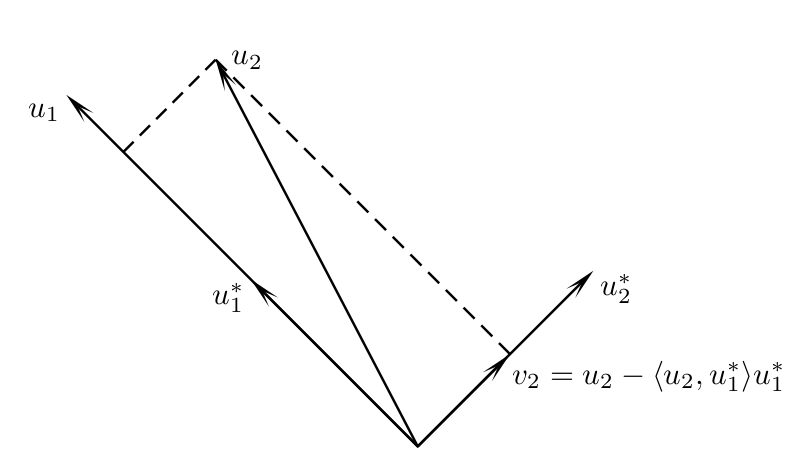
\includegraphics[width=0.5\textwidth]{images/gram_shmidt.png}
  \caption{格拉姆-施密特过程(5.13)的几何意义。这里 \(v_{n+1}\) 是将 \(u_{n+1}\) 投影到由标准正交基 \((u_1^*, u_2^*, \ldots, u_n^*)\) 
  张成的空间后的误差残差,而 \(u_{n+1}^*\) 是 \(v_{n+1}\) 的标准化。另见定义 5.26 和例子 5.27。}
  \label{fig::gram_shmidt}
\end{figure}

\hl{推论 5.22} 对于有限或无限独立的列表 \((u_1, u_2, \ldots)\),我们可以找到常数
\[
\begin{array}{ccc}
b_{11} &&\\
b_{21} & b_{22}& \\
b_{31} & b_{32} & b_{33} \\
\vdots
\end{array}
\]

以及一个标准正交列表 \((u_1^*, u_2^*, \ldots)\),使得 \(b_{ii} > 0\) 且
\begin{align*}
& u_1 = b_{11} u_1^* \\
& u_2 = b_{21} u_1^* + b_{22} u_2^* \\
& u_3 = b_{31} u_1^* + b_{32} u_2^* + b_{33} u_3^*
\end{align*}

\begin{proof}
这遵循(5.14)以及具有正对角线元素的下三角矩阵是可逆的。
\end{proof}

\hl{推论 5.23} 在定理 5.20 中,我们有 \(\langle u_n^*, u_i \rangle = 0\) 对于每个 \(i = 1, 2, \ldots, n-1\).

\begin{proof}
根据推论 5.22,每个 \(u_i\) 可以表示为
\[
  u_i = \sum_{k=1}^i b_{ik} u_k^*.
\]
将上述方程与 \(u_n^*\) 内积,应用正交条件,我们得到结论。
\end{proof}

% \hl{备注 5.9} 为了继续图 5.1 中的几何解释,推论 5.23 表明 \(u_i\) 和 \(u_i^*\) 张成相同的空间。
% 由于 \(u_n^*\) 对于每个 \(i = 1, 2, \ldots, n-1\) 与 \(u_i^*\) 垂直,所以它也与每个 \(u_i\) 垂直。


% \hl{定义 5.9} 内积空间 $X$ 的子集 $S$ 称为是标准正交的, 如果
% $$
% \forall u, v \in S, <u, v> = \left\{
% \begin{array}{ll}
%   1, & u = v,\\
%   0, & u \neq v.
% \end{array}
% \right.
% $$

% \hl{例 5.10} 空间 $\mathbb{R}^n$ 的一个标准正交基是一个标准正交的.

% \hl{定义 2.41} 第一类 Chebyshev 多项式定义为
% $$
% T_n : [-1, 1] \to [-1, 1], T_n(x) = \cos(n\arccos(x)).
% $$

% \hl{例 5.11} 定义 2.41 中给出的第一类 Chebyshev 多项式关于定理 5.7 中的内积定义是标准正交的, 这里取 
% $$
% a = -1, b = 1, \rho(x) = \frac{1}{\sqrt{1 - x^2}}.
% $$
% 对第二类 Chebyshev 多项式, 内积的权函数要取的不同. 见后.
% (验证一下? 对 $\rho(x)$ 做变量替换, 所以 $\rho(x)$ 是剧情需要.)

% 标准正交化中的正交指向量两两正交, 标准指向量的模长都是 $1$. 正交系可以通过规范化变成标准正交系. 

% \hl{定理 5.12} 有限个标准正交的向量组是线性无关组. 

% \hl{定义 5.13} (Gram-Schmidt 过程) 输入内积空间线性无关向量组 $(u_1, u_2, \cdots)$, 可以是无穷个. 输出 $(v_1, v_2, \cdots)$
% 和 $(u^*_1, u^*_2, \cdots)$, 具体过程为:
% $$
% \begin{array}{rcl}
%   v_1 &=& u_1, \\
%   u^*_1 &=& v_1 / \|v_1\|, \\
%   v_{n + 1} &=& u_{n + 1} - \sum_{k = 1}^n <u_{n + 1}, u^*_k> u^*_k,  n = 1, 2, \cdots\\
%   u^*_{n + 1} &=& v_{n + 1} / \|v_{n + 1}\|, n = 1, 2, \cdots .
% \end{array}
% $$

% 这个过程就是我们代数中学过的 Schmidt 正交化. 它将一组非正交的线性无关组 $(u_1, u_2, \cdots)$ 改造成一组标准正交组
% $(u^*_1, u^*_2, \cdots)$. 这里 $(v_1, v_2, \cdots)$ 正交但没有归一化. 

% \hl{定理 5.14} 这个定理结论是
% $$
% \begin{array}{rcl}
%   u^*_1 &=& a_{11}u_1 \\
%   u^*_2 &=& a_{21}u_1 + a_{22}u_2\\
%   u^*_3 &=& a_{31}u_1 + a_{32}u_2 + a_{33}u_3\\
%   &\vdots&
% \end{array}
% $$
% 是标准正交的, 这里 $a_{ij}$ 是常数, $i = 1, 2, \cdots$, $j = 1, 2, \cdots, i$. 
% 另外一个平凡的结论是, $u^*_n$ 只和 $u_1$, $u_2$, $\cdots$, $u_n$ 相关. 具体的证明过程是 Schmidt 正交化的重复, 
% 不再复述.

% \hl{例题 5.15} 这道题旨在解释 Schmidt 正交化的几何意义. 已知 $u^*_1$, $u^*_2$, $\cdots$, $u^*_n$ 已经标准正交, 
% 现在 $u_{n + 1}$ 和 $u^*_1$, $u^*_2$, $\cdots$, $u^*_n$ 均线性无关 (这一点由输入的 $u_1$, $u_2$, $\cdots$ 线性无关保证),
% 所以 $u_{n + 1}$ 在减去它在 $u^*_1$, $u^*_2$, $\cdots$, $u^*_n$ 等维度上的投影以后, 也即
% $$
% v_{n + 1} = u_{n + 1} - \sum_{k = 1}^n <u_{n + 1}, u^*_k> u^*_k 
% $$
% 是 $u_{n + 1}$ 在空间 
% $$
% \mbox{span}\{u^*_1, u^*_2, \cdots, u^*_n, u_{n + 1}\}
% $$
% 正交投影后的剩余部分, 或者误差. 

% \hl{推论 5.16} 定理 5.14 的结论可以反过来, 这个是显然的, 因为标准正交系是一组基.

% \hl{推论 5.17} 这个结论尽管简单, 但直观很重要. 
% $$
% u_i = \sum_{k = 1}^i b_{ik} u^*_k
% $$ 
% 也就是说 $u_i$ 已经全部分解到 $u^*_1$, $u^*_2$, $\cdots$, $u^*_i$ 上了, 
% 对任何 $u^*_j$, $j > i$, $u_i$ 在上面的投影必为零.

% \hl{定义 5.18} 对我们最熟悉的多项式空间基 $(1, x, x^2, \cdots)$ 在对应的内积下做 Gram-Schmidt 标准正交化, 
% 就得到表中的各组正交多项式系. 包括我们以及知道的第一类和第二类的 Chebyshev 多项式. 
% 表中给出了具体的积分区间 $[a, b]$ (可以是无穷) 和权函数. 这些正交多项式系由于其良好的性质,
% 在各种数值算法中有应用. 但注意, Schmidt 正交化虽然可以定义这些正交系, 
% 但实际计算我们一般不这么做, 而是采用递推公式, 比如第一类 Chebyshev 多项式, 
% 我们可以用递推公式 (2.43).

% \hl{例 5.19} 这个例子大家应该算一遍, 但要知道实际工作不这么做, 这个专门用于考试. 
% 各正交多项式系的公式可以在各种工程数学用表中查到. 不过如果一定要做 Schmidt 正交化, 
% 那么积分时注意利用区间对称性和函数奇偶性.


\hl{定义 5.24} 使用格拉姆-施密特正交化过程以及内积(5.6),我们从独立的单项式列表 $(1, x, x^2, \cdots)$ 获得以下经典的正交多项式:

\[
\begin{array}{|c|c|c|c|}
\hline
\text{多项式类型} & a & b & \rho(x) \\
\hline
\text{第一类切比雪夫多项式} & -1 & 1 & \frac{1}{\sqrt{1-x^2}} \\
\text{第二类切比雪夫多项式} & -1 & 1 & \sqrt{1-x^2} \\
\text{勒让德多项式} & -1 & 1 & 1 \\
\text{雅可比多项式} & -1 & 1 & (1-x)^\alpha(1+x)^\beta \\
\text{拉盖尔多项式} & 0 & +\infty & x^\alpha e^{-x} \\
\hline
\end{array}
\]
其中 \(\alpha, \beta > -1\) 对于雅可比多项式,以及 \(\alpha > -1\) 对于拉盖尔多项式。

\hl{例子 5.25} 我们使用格拉姆-施密特过程计算前三个勒让德多项式。

\begin{align*}
u_1 &= 1, \, v_1 = 1, \|v_1\|^2 = \int_{-1}^{+1} dx = 2, \quad u_1^* = \frac{1}{\sqrt{2}}. \\
u_2 &= x, \, v_2 = x - \left\langle x, \frac{1}{\sqrt{2}} \right\rangle \frac{1}{\sqrt{2}} = x, \, \|v_2\|^2 = \frac{2}{3}, \\
u_2^* &= \sqrt{\frac{3}{2}} x. \\
v_3 &= x^2 - \left\langle x^2, \sqrt{\frac{3}{2}} x \right\rangle \sqrt{\frac{3}{2}} x - \left\langle x^2, \frac{1}{\sqrt{2}} \right\rangle \frac{1}{\sqrt{2}} 
= x^2 - \frac{1}{3}, \\
\|v_3\|^2 &= \int_{-1}^{+1} \left(x^2 - \frac{1}{3}\right)^2 dx = \frac{8}{45}, \\
u_3^* &= \frac{3}{4} \sqrt{10} \left(x^2 - \frac{1}{3}\right).
\end{align*}


\hl{备注 5.10} 对于区间 \([-1,+1]\),通过检查函数是奇函数还是偶函数,可以加快其上积分的计算速度。

\subsubsection{傅里叶展开}
% 5.2.3 

\hl{备注 5.11} 由于 $2$-范数作为 ``长度'' 的度量,正交系统导致正交展开。注意,正交归一系统不需要是正交归一基,因为对于任何子空间,最佳逼近都是有意义的。

\hl{定义 5.26} 设 \((u_1^*, u_2^*, \ldots)\) 是有限或无限标准正交基。对于任意 \(w\),其正交展开或傅里叶展开是级数
\[
  \sum_{n=1}^m \langle w, u_n^* \rangle u_n^*,
\]
其中常数 \(\langle w, u_n^* \rangle\) 被称为 \(w\) 的傅里叶系数,而项 \(\langle w, u_n^* \rangle u_n^*\) 是 \(w\) 在 \(u_n^*\) 上的投影。
\(w\) 关于 \((u_1^*, u_2^*, \ldots)\) 的傅里叶展开的误差仅仅是 \(\sum_{n} \langle w, u_n^* \rangle u_n^* - w\).
(就是 $w$ 在 $\mathrm{span}\{u_1^*, u_2^*, \ldots\}$ 空间的正交投影。)


\hl{例子 5.27} 使用定义 B.169 中的欧几里得内积,我们选择 \(\mathbb{R}^3\) 中的正交归一向量为
\[
  u_1^* = (1,0,0)^T, \, u_2^* = (0,1,0)^T, \, u_3^* = (0,0,1)^T.
\]

对于向量 \(w = (a, b, c)^T\),傅里叶系数为
\[
  \langle w, u_1^* \rangle = a, \, \langle w, u_2^* \rangle = b, \, \langle w, u_3^* \rangle = c,
\]

且 \(w\) 在 \(u_1^*\) 和 \(u_2^*\) 上的投影为
\[
  \langle w, u_1^* \rangle u_1^* = (a,0,0)^T, \quad \langle w, u_2^* \rangle u_2^* = (0,b,0)^T.
\]

\(w\) 的傅里叶展开为
\[
  w = \langle w, u_1^* \rangle u_1^* + \langle w, u_2^* \rangle u_2^* + \langle w, u_3^* \rangle u_3^*,
\]
傅里叶展开的误差为 $0$;因为 $w \in \mathbb{R}^3$.

\hl{备注 5.12} 对于正交基 \(u_i\) ,我们可以通过 \(u_i^* = u_i / \|u_i\|\) 构造一个标准正交基,以得到傅里叶展开
\[
  w \sim \sum_i \langle w, \frac{u_i}{\|u_i\|} \rangle \frac{u_i}{\|u_i\|} = \sum_i \frac{\langle w, u_i \rangle}{\langle u_i, u_i \rangle}.
\]

这里我们使用 ``$\sim$'' 而不是 ``='' 是因为对于无限序列 \((u_i)_{i \in \mathbb{N}}\),级数可能不收敛。(在无穷维,这么做可能失败。)

\hl{练习 5.28} 对于 \(L_{\rho=1}^{2}[-\pi,\pi]\) 中的标准正交基,
\[
  \frac{1}{\sqrt{2\pi}}, \frac{\sin x}{\sqrt{\pi}}, \frac{\cos x}{\sqrt{\pi}}, \ldots, \frac{\sin(nx)}{\sqrt{\pi}}, \frac{\cos(nx)}{\sqrt{\pi}}, \ldots, \tag{5.19}
\]
导出函数 \(f(x)\) 的傅里叶级数为
\[
  f(x) \sim \frac{a_0}{2} + \sum_{k=1}^{+\infty} (a_k \cos kx + b_k \sin kx), \tag{5.20}
\]
其中系数为
\[
  a_k = \frac{1}{\pi} \int_{-\pi}^\pi f(x) \cos kx \, dx, \, b_k = \frac{1}{\pi} \int_{-\pi}^\pi f(x) \sin kx \, dx.
\]
(这就是我们在实分析中熟悉的傅里叶展开。)


\hl{备注 5.13} 假设有限维标准正交基 \((u_1^*, u_2^*, \ldots)\) 是有限的,那么这个列表张成空间中的任何线性组合都等于其傅里叶展开。这与备注 5.12 相比较。

\hl{定理 5.29} 设 \(u_1, u_2, \ldots, u_n\) 是线性无关的,并且 \(u_i^*\) 是通过格拉姆-施密特过程正交归一化的 \(u_i\). 
如果 \(w = \sum_{i=1}^{n} a_i u_i\),那么
\[
  w = \sum_{i=1}^n \langle w, u_i^* \rangle u_i^*, \tag{5.21}
\]
即 \(w\) 等于其傅里叶展开。

\begin{proof}
根据条件 \(w = \sum_{i=1}^{n} a_i u_i\) 和推论 5.22,我们可以将 \(w\) 表达为 \(u_i^*\) 的线性组合,
即 \(w = \sum_{i=1}^{n} c_i u_i^*\)。然后 \(u_i^*\) 的正交归一性意味着
\[
  \forall k = 1, 2, \cdots, n, \quad \langle w, u_k^* \rangle = c_k,
\]
这完成了证明。
\end{proof}

\hl{备注 5.14} 从逼近的角度来看,对于 \(w \in \operatorname{span}(u_1, u_2, \ldots, u_n)\), 
使用 \(u_1, u_2, \ldots, u_n\) 的某些线性组合对 \(w\) 进行最佳逼近的误差为零。
这也推广到 \(w \notin \operatorname{span}(u_1, u_2, \ldots, u_n)\) 的情况。

\hl{定理 5.30}(傅里叶展开的最小性质)。设 \(u_1^*, u_2^*, \ldots\) 是一个正交归一系统,并且让 \(w\) 是任意的。那么
\[
  \left\| w - \sum_{i=1}^N \langle w, u_i^* \rangle u_i^* \right\| \leq \left\| w - \sum_{i=1}^N a_i u_i^* \right\|, \tag{5.22}
\]
对于任意常数选择 \(a_1, a_2, \cdots, a_N\)。(注意这里的范数都是$2-$范数。)

\begin{proof}
使用简写符号 \(\sum_i = \sum_{i = 1}^{N}\), 我们从内积的定义和性质推导出
\begin{align*}
  &\left\| w - \sum_i a_i u_i^* \right\|^2 = \left\langle w - \sum_i a_i u_i^*, w - \sum_i a_i u_i^* \right\rangle \\
  &= \langle w, w \rangle - \left\langle w, \sum_i a_i u_i^* \right\rangle - \left\langle \sum_i a_i u_i^*, w \right\rangle \\
  &\quad + \left\langle \sum_i a_i u_i^*, \sum_i a_i u_i^* \right\rangle \\
  &= \langle w, w \rangle - \sum_i \overline{a_i} \langle w, u_i^* \rangle - \sum_i a_i \langle u_i^*, w \rangle \\
  &\quad + \sum_i \sum_j a_i \overline{a_j} \langle u_i^*, u_j^* \rangle \\
  &= \langle w, w \rangle - \sum_i \overline{a_i} \langle w, u_i^* \rangle - \sum_i a_i \langle u_i^*, w \rangle + \sum_i |a_i|^2 \\
  &\quad - \sum_i \langle u_i^*, w \rangle \langle w, u_i^* \rangle + \sum_i \langle u_i^*, w \rangle \langle w, u_i^* \rangle \\
  &= \left\| w \right\|^2 - \sum_i \left| \langle w, u_i^* \rangle \right|^2 + \sum_i \left| a_i - \langle w, u_i^* \rangle \right|^2,
\end{align*}
其中 ``$|\cdot|$'' 表示复数的模。前两项与 \(a_i\) 无关。因此 \(\left\| w - \sum_i a_i u_i^* \right\|^2\) 仅在 \(a_i = \langle w, u_i^* \rangle\) 
时取得最小值。
\end{proof}
(记 $V = \mathrm{span}\{u^*_1, u^*_2, \cdots\}$,任取 $w' \in V$, 那么误差 $e = w - w'$ 在该空间的正交投影记作 $e^*$ 是
$$
e^* = \sum \langle w - w', u_i^* \rangle u_i^* =  \sum \langle w, u_i^* \rangle u_i^* + \sum \langle w', u_i^* \rangle u_i^*.
$$
注意上式第一部分就是证明需要的 $w$ 在 $V$ 的最佳逼近元,记作 $w^*$. 而第二部分注意到 $w' \in V$, 因此就是 $w'$ 本身。即
$$
e^* = w^* - w'
$$
于是 
$$
\|w - w'\| = \|w - w^* + e^*\| \leq \|w - w^*\| + \|e^*\|.
$$
当 $\|e^*\| = 0$ 时取到最小,而此时,$w^* = w'$. 这个定理的意义是,正交投影其实是一种分解,$w$ 被分解成一个空间内的元素 $w^*$ 
和一个已经无法用空间信息表达的误差 $e$,因此这个正交投影对于该空间而言是最佳的。)

\hl{备注 5.15} 作为图 5.1 关于格拉姆-施密特过程几何意义的延续,
定理 5.30 指出 \(\left\|v_{n+1}\right\|\) 是用其在由 \((u_1^*, \ldots, u_n^*)\) 张成的空间上的投影来逼近 \(u_{n+1}\) 时的最小误差。

\hl{推论 5.31} 设 \((u_1, u_2, \ldots, u_n)\) 是一组基,
线性逼近任意向量 \(w\) 的基本问题通过最佳逼近 \(\hat{\varphi} = \sum_{k} \langle w, u_k^* \rangle u_k^*\) 来解决,
其中 \(u_k^{*}\) 是通过格拉姆-施密特过程正交归一化的 \(u_k^*\)。误差范数是
\[
  |w - \hat{\varphi}|^2 := \min_{a_k} \left\|w - \sum_{k=1}^n a_k u_k\right\|^2 = \|w\|^2 - \sum_{k=1}^n \left|\langle w, u_k^* \rangle\right|^2.
\]
\begin{proof}
这直接来自 (5.23)。  
\end{proof}

\hl{推论 5.32}(贝塞尔不等式)如果 \(u_1^*, u_2^*, \ldots, u_N^*\) 是标准正交的,那么对于任意 \(w\),
\[
  \sum_{i=1}^N \left|\langle w, u_i^* \rangle\right|^2 \leq \|w\|^2. \tag{5.25}
\]

\begin{proof}
这直接来自推论 5.31 和范数的实正性。
\end{proof}

\hl{推论 5.33} 定义 5.19 中的格拉姆-施密特过程满足
\[
  \forall n \in \mathbb{N}^+, \quad \left\|v_{n+1}\right\|^2 = \left\|u_{n+1}\right\|^2 - \sum_{k=1}^n \left|\langle u_{n+1}, u_k^* \rangle\right|^2. \tag{5.26}
\]
\begin{proof}
根据 (5.13a),每个 \(v_{n+1}\) 可以被视为 \(u_{n+1}\) 相对于标准正交 \((u_1^*, u_2^*, \ldots, u_n^*)\) 的傅里叶展开的误差。
在推论 5.31 中,将 \(w\) 与 \(u_{n+1}\) 识别完成证明。
\end{proof}

\hl{备注 5.16} 傅里叶展开在两个方面帮助我们理解格拉姆-施密特过程:
\begin{itemize}
  \item 定义 5.19 是傅里叶展开的一种特殊类型;这有助于记忆。
  \item 作为定义 5.19 和定理 5.20 的补充,推论 5.33 揭示了向量 \(u_k, v_k\) 和 \(u_k^*\) 之间的额外关系。
\end{itemize}

\hl{例子 5.34} 考虑例子 5.4 中的最小二乘逼近问题,权重函数 \(\rho=1\)。它等价于
\[
  \min_{a_i} \int_{-1}^{+1} \left(e^x - \sum_{i=0}^n a_i x^i\right)^2 dx.
\]

对于 \(n=1,2\),使用例子 5.25 中导出的勒让德多项式:
\[
  u_1^* = \frac{1}{\sqrt{2}}, \, u_2^* = \sqrt{\frac{3}{2}} x, \, u_3^* = \frac{1}{4} \sqrt{10} (3x^2 - 1).
\]

我们得到 \(e^x\) 的傅里叶系数为

\begin{align*}
b_1 &= \int_{-1}^{+1} \frac{1}{\sqrt{2}} e^x \, dx = \frac{1}{\sqrt{2}} \left(e - \frac{1}{e}\right), \\
b_2 &= \int_{-1}^{+1} \sqrt{\frac{3}{2}} x e^x \, dx = \sqrt{6} e^{-1}, \\
b_3 &= \int_{-1}^{+1} \frac{1}{4} \sqrt{10} (3x^2 - 1) e^x \, dx = \frac{\sqrt{10}}{2} \left(e - \frac{7}{e}\right).
\end{align*}

因此,最小化多项式为

\[
\hat{\varphi}_n = \begin{cases}
\frac{1}{2e}(e^2 - 1) + \frac{3}{e}x & \text{如果 } n = 1; \\
\hat{\varphi}_1 + \frac{5}{4e}(e^2 - 7)(3x^2 - 1) & \text{如果 } n = 2.
\end{cases} \tag{5.28}
\]
\hl{备注 5.17} 例子 5.34 展示了在解决最小二乘逼近问题时正交归一系统的性能优势:
低阶最佳逼近的傅里叶系数可以并且应该在构建高阶最佳逼近时重复使用。这类似于牛顿法相对于拉格朗日公式的优势。



% \subsubsection{傅立叶展开, Fourier expansions}

% \hl{定义 5.20} 傅立叶展开. 令 $(u^*_1, u^*_2, \cdots)$ 是有限或无限的标准正交系,
% 对任意的向量 $w$, 其傅立叶展开或正交展开为
% $$
% \sum_{n = 1}^m <w, u^*_n>u^*_n.
% $$
% 这里 $<w, u^*_n>$ 称为傅立叶系数. 而 $w$ 关于 $(u^*_1, u^*_2, \cdots)$ 
% 的傅立叶展开的误差为:
% $$
% \sum_{n = 1}^m <w, u^*_n>u^*_n - w.
% $$
% 这里 $<w, u^*_n> u^*_n$ 的几何意义为 $w$ 在 $u^*_n$ 的投影.

% \hl{例 5.21} 傅立叶展开是和内积空间相关的. 我们可以对任意 $w \in \mathbb{R}^3$ 
% 空间, 关于欧氏内积对标准正交基 $(1, 0, 0)^T$, $(0, 1, 0)^T$ 和 $(0, 0, 1)^T$ 
% 做傅立叶展开, 得到的系数就是标准坐标. 所以展开误差是 $0$.

% 对于非标准(没有规一化)的正交组 $(u_1, u_2, \cdots)$, 我们可以直接通过归一化
% $u^*_i = u_i / \|u_i\|$, $i = 1, 2, \cdots$ 后再得到任意向量 $w$ 的傅立叶展开:
% $$
% w \sim \sum_i \left<w, \frac{u_i}{\|u_i\|}\right>\frac{u_i}{\|u_i\|}
% = \sum_i\frac{<w, u_i>}{<u_i, u_i>}u_i.
% $$
% 注意 
% $$
% <u_i, u_i> = \|u_i\|^2.
% $$
% 这里使用 $\sim$ 而不是 $=$, 是因为对于无穷项标准正交系, 求和式不一定收敛. 

% \hl{例题 5.22} 对 $f \in L_{\rho = 1}^2[-\pi, \pi]$ 关于其上的标准正交系
% $$
% \frac{1}{\sqrt{2\pi}}, \frac{\sin x}{\sqrt{\pi}}, \frac{\cos x}{\sqrt{\pi}}, 
% \frac{\sin 2x}{\sqrt{\pi}}, \frac{\cos 2x}{\sqrt{\pi}}, \cdots,
% \frac{\sin nx}{\sqrt{\pi}, \frac{\cos nx}{\sqrt{\pi}}}, \cdots,
% $$
% 做傅立叶展开, 就是我们熟悉的傅立叶级数:
% $$
% f(x) \sim \frac{a_0}{2} + \sum_{k = 1}^{\infty}(a_k \cos kx + b_k \sin kx),
% $$
% 其中
% $$
% a_k = \frac{1}{\pi}\int^\pi_{-\pi} f(x) \cos kx dx, 
% b_k = \frac{1}{\pi}\int^\pi_{-\pi} f(x) \sin kx dx. 
% $$

% 如果标准正交系是有限个, 那么傅立叶展开就是在这组正交系下的线性表出.

% \hl{定理 5.23} 令 $(u_1, u_2, \cdots, u_n)$ 线性无关, 而 $u^*_i$ 是 $u_i$ 做 
% Gram-Schmidt 正交化后的输出. 如果
% $$
% w = \sum_{i = 1}^n u_i,
% $$
% 那么
% $$
% w = \sum_{i = 1}^n <w, u^*_i> u^*_i,
% $$
% 也即有限维的傅立叶展开总是收敛且相等的.

% \hl{证明: } 因为 $(u^*_1, u^*_2, \cdots, u^*_n)$ 是一组标准正交基, 故令
% $$
% w = \sum_{i = 1}^n c_i u^*_i,
% $$
% 于是
% $$
% <w, u^*_k> = \sum_{i = 1}^n c_i <u^*_i, u^*_k>,
% $$
% 由正交性,
% $$
% <u^*_i, u^*_k> = \delta_{ik}, 
% $$
% 所以 $<w, u^*_k> = c_k$, 证毕. $\qed$

% 从最佳逼近的角度看, 以上操作就是 $w \in \mbox{span}(u_1, u_2, \cdots, u_n)$
% 的最佳逼近, 而且误差是零. 当 $w \notin \mbox{span}(u_1, u_2, \cdots, u_n)$
% 时, 该最佳逼近公式仍然成立. 

% \hl{定理 5.24} 傅立叶展开的最小性质. 令 $(u^*_1, u^*_2, \cdots)$ 是一组标准正交基,
% 而 $w$ 是任意向量. 则
% $$
% \left\|w - \sum_{i = 1}^N <w, u^*_i> u^*_i\right\| 
% \leq \left\|w - \sum_{i = 1}^N a_i u^*_i\right\|,
% $$
% 对任意常数序列 $a_1$, $a_2$, $\cdots$, $a_N$ 成立.

% 这个证明其实很简单, 直接对
% $$
% \left\|w - \sum_{i = 1}^N a_i u^*_i\right\|^2
% $$
% 做展开后整理成
% $$
% \left\|w - \sum_{i = 1}^N a_i u^*_i\right\|^2 
% = \|w\|^2 - \sum_i|<w, u^*_i>|^2 + \sum_i|a_i - <w, u^*_i>|^2,
% $$
% 显然当 
% $$
% \sum_i|a_i - <w, u^*_i>|^2 = 0
% $$
% 时取极小, 也即 $a_i = <w, u^*_i>$, $i = 1, 2, \cdots, N$.

% \hl{推论 5.25} 令 $(u_1, u_2, \cdots, u_n)$ 是线性无关组, 则任意向量 $w$ 的基本最佳逼近问题的解为
% $\hat{\phi} = \sum_k <w, u^*_k> u^*_k$, 其中 $u^*_k$ 是 $u_k$ 的 Gram-Schmidt 正交化过程对应的输出. 
% 而误差的范数为
% $$
% \|w - \hat{\phi}\|^2 := \min_{a_k} \|w - \sum_{k = 1}^n a_k u_k\|^2 
% = \|w\|^2 - \sum_{k = 1}^n|<w, u^*_k>|^2.
% $$

% 这个就是定理 5.24 结论的重复叙述.

% \hl{推论 5.26} 贝塞尔不等式, Bessel inequality. 如果 $(u^*_1, u^*_2, \cdots, u^*_N)$ 是标准正交系, 
% 则对任意向量 $w$, 有
% $$
% \sum_{i = 1}^N |<w, u^*_i>|^2 \leq \|w\|^2.
% $$
% 就看 $w$ 在不在空间内了.

% \hl{推论 5.27} Gram-Schmidt 正交化过程满足
% $$
% \|v_{n + 1}\|^2  = \|u_{n + 1}\|^2 - \sum_{k = 1}^n|<u_{n + 1}, u^*_k>|^2.
% $$
% 这是将 $v_{n + 1}$ 看作是 $u_{n + 1}$ 关于 $(u^*_1, u^*_2, \cdots, u^*_n)$ 做投影后的误差.

% \hl{例题 5.28} 我们来考虑如何做最佳平方逼近. 比如将 $e^x$, 在 $[-1, 1]$ 上用直到 $2$ 次的多项式逼近. 
% 或者说, 求
% $$
% \min_{a_i} \int^1_{-1}\left(e^x - \sum_{i = 1}^2a_i x^i\right)^2 dx.
% $$
% 我们直接给出 $[-1, 1]$ 上 $\rho = 1$ 的正交多项式系, 也就是 Legenfre 多项式, 由例题 5.19,
% $$
% u^*_1 = \frac{1}{\sqrt{2}}, u^*_2 = \sqrt{\frac{3}{2}}x, u^*_3 = \frac{1}{4}\sqrt{10}(3x^2 - 1).
% $$ 
% (直到 $2$ 次.) 然后对 $e^x$ 求在这些正交系上的表出系数, 或傅立叶展开系数:
% $$
% \begin{array}{rcl}
%   a_1 &=& \int^1_{-1} \frac{1}{\sqrt{2}} e^x dx = \frac{1}{\sqrt{2}}\left(e - \frac{1}{e}\right) \\
%   a_2 &=& \int^1_{-1} \sqrt{\frac{3}{2}}x e^x dx = \sqrt{6}\frac{1}{e}\\
%   a_3 &=& \int^1_{-1} \frac{1}{4}\sqrt{10}(3x^2 - 1) e^x dx = \frac{\sqrt{10}}{2}\left(e - \frac{7}{e}\right)
% \end{array}
% $$
% 最终结果是
% $$
% \begin{array}{rcl}
%   \hat{\phi} &=& a_1 u^*_1 + a_2 u^*_2 + a_3 u^*_3 \\
%   &=& \frac{1}{2e}(e^2 - 1) + \frac{3}{e} x + \frac{5}{4e} (e^2 - 7)(3 x^2 - 1)
% \end{array}
% $$
% 一般意义下的最佳平方逼近也是容易的.

\subsection{正规方程组}
% 5.3 

\hl{注释 5.18} 对于一个标准正交系, 我们可以很容易地通过计算给定函数 \( w \) 与列表元素的内积来找到最佳线性逼近, 
如示例 5.34 所示。如果列表不是标准正交的, 而只是线性无关的, 则一种方法是通过正规方程组得到最佳逼近, 这些方程在本小节推导。

\hl{定理 5.35} 设 \( u_{1}, u_{2}, \ldots, u_{n} \in X\) 是线性无关的, 并设 \( u_{i}^{*}\) 是由格拉姆-施密特过程对 \( u_{i}\) 归一化的。
那么, 对于任何元素 \( w \),
\[
  \forall j=1,2, \ldots, n, \quad\left(w-\sum_{k=1}^{n}\langle w, u_{k}^{*}\rangle u_{k}^{*}\right) \perp u_{j}^{*},
\]
其中 ``\(\perp\)'' 表示正交。

\begin{proof}
如果 \( w \in X \), 我们有 \( w-\sum_{k=1}^{n}\langle w, u_{k}^{*}\rangle u_{k}^{*}=0\) , 
因此(5.29)显然成立。对于另一种情况 \( w \notin X \),设置 \( w=u_{n+1}\) , 应用(5.16),我们得到(5.29)。
证毕。
\end{proof}

\hl{推论 5.36} 设 \( u_{1}, u_{2}, \ldots, u_{n} \in X\) 是线性无关的。如果 \(\hat{\varphi}=\sum_{k=1}^{n} a_{k} u_{k}\) 是到 \( w \) 的最佳线性逼近,则
\[
  \forall j=1,2, \ldots, n, \quad(w-\hat{\varphi}) \perp u_{j} .
\]
\begin{proof}
因为 \(\hat{\varphi}=\sum_{k=1}^{n} a_{k} u_{k}\) 是到 \( w \) 的最佳线性逼近, 定理 5.30 意味着
\[
  \sum_{k=1}^{n} a_{k} u_{k}=\sum_{k=1}^{n}\langle w, u_{k}^{*}\rangle u_{k}^{*}.
\]
推论 5.22 和定理 5.35 完成了证明。
\end{proof}

\noindent \textbf{定义 5.37} 设 $u_1, u_2, \ldots, u_n$ 是内积空间中的一组元素。定义 $n \times n$ 矩阵
\begin{align*}
G &= G(u_1, u_2, \cdots, u_n) = \left( \langle u_i, u_j \rangle \right) \\
& = \begin{bmatrix}
\langle u_1, u_1 \rangle & \langle u_1, u_2 \rangle & \cdots & \langle u_1, u_n \rangle \\
\langle u_2, u_1 \rangle & \langle u_2, u_2 \rangle & \cdots & \langle u_2, u_n \rangle \\
\vdots & \vdots & \ddots & \vdots \\
\langle u_n, u_1 \rangle & \langle u_n, u_2 \rangle & \cdots & \langle u_n, u_n \rangle
\end{bmatrix} \\
\end{align*}
是 $u_1, u_2, \ldots, u_n$ 的Gram矩阵。它的行列式
\[
g = g(u_1, u_2, \ldots, u_n) = \det \left( \langle u_i, u_j \rangle \right)
\]
是Gram行列式。

\noindent \textbf{引理 5.38.} 设 $w_i = \sum_{j=1}^n a_{ij} u_j$, 其中 $i = 1, 2, \ldots, n$. 
令 $A = (a_{ij})$, 其共轭转置为 $A^H = (\overline{a_{ji}})$. 则有
\[
  G(w_1, w_2, \ldots, w_n) = A G(u_1, u_2, \ldots, u_n) A^H
\]
并且
\[
  g(w_1, w_2, \ldots, w_n) = |\det A|^2 g(u_1, u_2, \ldots, u_n).
\]

\begin{proof}
$u_i$ 与 $w_j$ 的内积构成
\begin{align*}
\begin{bmatrix}
\langle u_1, w_1 \rangle & \langle u_1, w_2 \rangle & \cdots & \langle u_1, w_n \rangle \\
\langle u_2, w_1 \rangle & \langle u_2, w_2 \rangle & \cdots & \langle u_2, w_n \rangle \\
\vdots & \vdots & \ddots & \vdots \\
\langle u_n, w_1 \rangle & \langle u_n, w_2 \rangle & \cdots & \langle u_n, w_n \rangle
\end{bmatrix}
= &\begin{bmatrix}
\langle u_1, u_1 \rangle & \langle u_1, u_2 \rangle & \cdots & \langle u_1, u_n \rangle \\
\langle u_2, u_1 \rangle & \langle u_2, u_2 \rangle & \cdots & \langle u_2, u_n \rangle \\
\vdots & \vdots & \ddots & \vdots \\
\langle u_n, u_1 \rangle & \langle u_n, u_2 \rangle & \cdots & \langle u_n, u_n \rangle
\end{bmatrix} 
\begin{bmatrix}
a_{11} & \cdots & a_{1n} \\
a_{12} & \cdots & a_{2n} \\
\vdots & \ddots & \vdots \\
a_{1n} & \cdots & a_{nn}
\end{bmatrix} \\
=& G(u_1, u_2, \ldots, u_n) A^H。
\end{align*}

因此,(5.33) 成立,因为
\begin{align*}
G(w_1, w_2, \ldots, w_n) &= \begin{bmatrix}
\langle w_1, w_1 \rangle & \langle w_1, w_2 \rangle & \cdots & \langle w_1, w_n \rangle \\
\langle w_2, w_1 \rangle & \langle w_2, w_2 \rangle & \cdots & \langle w_2, w_n \rangle \\
\vdots & \vdots & \ddots & \vdots \\
\langle w_n, w_1 \rangle & \langle w_n, w_2 \rangle & \cdots & \langle w_n, w_n \rangle
\end{bmatrix} \\
&= \begin{bmatrix}
a_{11} & \cdots & a_{1n} \\
a_{21} & \cdots & a_{2n} \\
\vdots & \ddots & \vdots \\
a_{n1} & \cdots & a_{nn}
\end{bmatrix} 
\begin{bmatrix}
\langle u_1, u_1 \rangle & \langle u_1, u_2 \rangle & \cdots & \langle u_1, u_n \rangle \\
\langle u_2, u_1 \rangle & \langle u_2, u_2 \rangle & \cdots & \langle u_2, u_n \rangle \\
\vdots & \vdots & \ddots & \vdots \\
\langle u_n, u_1 \rangle & \langle u_n, u_2 \rangle & \cdots & \langle u_n, u_n \rangle
\end{bmatrix} 
\begin{bmatrix}
\overline{a_{11}} & \cdots & \overline{a_{n1}} \\
\overline{a_{12}} & \cdots & \overline{a_{n2}} \\
\vdots & \ddots & \vdots \\
\overline{a_{1n}} & \cdots & \overline{a_{nn}}
\end{bmatrix} \\
&= A G(u_1, u_2, \ldots, u_n) A^H。
\end{align*}

已知复共轭的性质为
\[
\overline{z + w} = \overline{z} + \overline{w}, \quad \overline{z w} = \overline{z} \, \overline{w}。
\]
因此,$\det A = \det A^T$ 和Leibniz行列式公式(定义 B.247)给出
\[
\det A = \det A^T = \sum_{\sigma \in S_n} \text{sgn}(\sigma) \prod_{i=1}^n a_{i, \sigma_i} = \det A^H。
\]
最后,由 (5.33) 的行列式和 $\det(AB) = \det A \det B$ 得出 (5.34)。
\end{proof}

\noindent \textbf{备注 5.19.} 引理 5.38 在证明以下定理中起到了关键作用。

\noindent \textbf{定理 5.39.} 对于非零元素 $u_1, u_2, \ldots, u_n \in X$, 我们有
\[
  0 \leq g(u_1, u_2, \ldots, u_n) \leq \prod_{k=1}^n \|u_k\|^2,
\]
其中,当且仅当 $u_1, u_2, \ldots, u_n$ 线性相关时取左等号,只有当它们正交时取右等号。

\begin{proof}
假设 $u_1, u_2, \ldots, u_n$ 线性相关。那么可以找到常数 $c_1, c_2, \ldots, c_n$ 满足 $\sum_{i=1}^n c_i u_i = 0$, 且至少有一个 $c_j$ 非零。构造向量
\[
  w_k = \begin{cases}
    \sum_{i=1}^n c_i u_i = 0, & k = j; \\
    u_k, & k \neq j。
  \end{cases}
\]
因为 $\langle w_j, w_k \rangle = 0$ 对每个 $k$ 都成立,所以 $g(w_1, w_2, \ldots, w_n) = 0$. 根据Laplace定理(定理 B.253),
我们可以通过 $C = (c_{ij})$ 的 $j$ 行的代数余子式展开行列式:
\[
  \det(C) = \det \begin{bmatrix}
    1 & 0 & \cdots & 0 & \cdots & 0 \\
    0 & 1 & 0 & \cdots & 0 \\
    \vdots & \vdots & \ddots & \vdots & \vdots & \vdots \\
    c_1 & c_2 & \cdots & c_j & \cdots & c_n \\
    \vdots & \vdots & \ddots & \vdots & \vdots & \vdots \\
    0 & 0 & \cdots & 0 & 1
  \end{bmatrix}
= 0 + \cdots + 0 + c_j + 0 + \cdots + 0 = c_j \neq 0,
\]
其中,$i \neq j$ 的每个余子式矩阵 $M_i$ 的行列式都为零,因为 $M_i$ 的 $i_0$ 行是由零组成的一行,
其中 $i_0 = i$ 当 $i < j$ 时,$i_0 = i - 1$ 当 $i > j$ 时。因此,$g(u_1, u_2, \ldots, u_n) = 0$.

假设 $u_1, u_2, \ldots, u_n$ 线性无关。根据定理 5.20,我们可以找到常数 $a_{ij}$ 使得 $a_{kk} > 0$ 且如下向量是正交的:
\[
  u_k^* = \sum_{i=1}^k a_{ki} u_i.
\]
那么根据定义 5.37,$g(u_1^*, u_2^*, \ldots, u_n^*) = 1$. 
此外,由于矩阵 $(a_{ij})$ 是上三角矩阵,我们有 $\det (a_{ij}) = \prod_{k=1}^n a_{kk}$. 由引理 5.38 可得
\[
  g(u_1, u_2, \ldots, u_n) = \prod_{k=1}^n \frac{1}{a_{kk}^2} > 0.
\]

由于向量列表 $(u_1, u_2, \ldots, u_n)$ 或线性相关或线性无关,前述论证表明 $g(u_1, u_2, \ldots, u_n) = 0$ 当且仅当 $u_1, u_2, \ldots, u_n$ 线性相关。

假设 $u_1, u_2, \ldots, u_n$ 是正交的。根据定义 5.37,$G(u_1, u_2, \ldots, u_n)$ 是一个对角矩阵,且对角线上的元素为 $\|u_k\|^2$. 
因此,$u_k$ 的正交性意味着
\[
  g(u_1, u_2, \ldots, u_n) = \prod_{k=1}^n \|u_k\|^2.
\]
\end{proof}

\subsection{正规方程组, the normal equations}
如果我们已经有一个标准正交系或者正交系, 那么最佳平方逼近只需要做内积就行了. 但是如果我们只有一组无关向量组, 
那么一般先做 Gram-Schmidt 正交化是一个昂贵的过程, 在具体问题的时候, 并不建议这么操作, 而是采用正规方程组.

\hl{定理 5.29} 令 $u_1, u_2, \cdots, u_n \in X$ 线性无关, 而 $u^*_i$ 是 $u_i$ 对应的 Gram-Schmidt 
正交化结果. 则对任意 $w$, 有
$$
\left(w - \sum_{k = 1}^n<w, u^*_k> u^*_k\right) \perp u^*_j , j = 1, 2, \cdots, n.
$$
这里 $\perp$ 是正交的意思, 所以这个定理只是推论 5.17 的另一种表述.

\hl{推论 5.30} 令 $u_1, u_2, \cdots, u_n \in X$ 线性无关, 如果 
$$
\hat{\phi} = \sum_{k = 1}^n a_k u_k
$$
是 $w$ 的最佳平方逼近, 则
$$
(w - \hat{\phi}) \perp u_j, j = 1, 2, \cdots, n.
$$
这一步也是显然的. 

现在我们可以准备处理一般基了. 

\hl{定义 5.31} 令 $u_1, u_2, \cdots, u_n$ 是向量空间中的一列向量组, 那么 $n \times n$ 矩阵
$$
\begin{array}{rcl}
  G &=& G(u_1, u_2, \cdots, u_n) = (<u_i, u_j>)\\
  &=& \begin{array}{cccc}
    <u_1, u_1> & <u_1, u_2> & \cdots & <u_1, u_n> \\
    <u_2, u_1> & <u_2, u_2> & \cdots & <u_2, u_n> \\
    \vdots & \vdots & \ddots & \vdots\\
    <u_n, u_1> & <u_n, u_2> & \cdots & <u_n, u_n>
  \end{array}  
\end{array}
$$
称为向量组 $u_1, u_2, \cdots, u_n$ 的 Gram 矩阵, 它的行列式
$$
g = g(u_1, u_2, \cdots, u_n) = det(G)
$$ 
称为 Gram 行列式.

\hl{引理 5.32} 令
$$
w_i = \sum_{j = 1}^n a_{ij} u_j , j = 1, 2, \cdots, n.
$$
($w_i$, $i = 1, 2, \cdots, n$ 是 $\mbox{span}(u_1, u_2, \cdots, u_n)$ 空间的 $n$ 个向量.)
记复矩阵 $A = (a_{ij})$ 的共轭转置为 $A^H = (\bar{a_{ji}})$, 则
$$
G(w_1, w_2, \cdots, w_n) = A G(u_1, u_2, \cdots, u_n) A^H,
$$
并且
$$
g(w_1, w_2, \cdots, w_n) = |det(A)|^2g(u_1, u_2, \cdots, u_n).
$$
这里 $|det(A)|$ 是 $A$ 的行列式 (是复数) 的模的平方. 该定理给出了向量在一般基表示和标准正交基表示下的关系.

\hl{证明} 考虑
$$
<u_i, w_j> = <u_i, \sum_{k = 1}^n a_{jk} u_k> = \sum_{k = 1}^n \bar{a_{jk}} <u_i, u_k>,
$$
(这里要考虑复数的内积性质) 有
$$
(<u_i, w_j>) = (<u_i, u_j>) A^H = G(u_1, u_2, \cdots, u_n) A^H.
$$
然后 
$$
<w_i, w_j> = <\sum_{k = 1}^n a_{ik} u_k, w_j> = \sum_{k = 1}^n a_{ik} <u_k, w_j>,
$$
即
$$
(w_i, w_j) = A (u_i, w_j).
$$
两式联合即有
$$
(w_i, w_j) = A (u_i, u_j) A^H.
$$
直接对该式两边做行列式, 即得 (5.29).

引理 5.32 就是为了证明下面的定理:

\hl{定理 5.33.} 对于非零元素 $u_1, u_2, ..., u_n \in X$, 
我们有
\[
0 \leq g(u_1 , u_2 , . . . , u_n ) \leq \prod_{k}^n ||u_k||^2,
\] 
其中, 当且仅当 $u_1, u_2, ..., u_n$ 线性相关且正交时, 左式等式成立, 
而当且仅当它们两两正交时, 右式等式成立.

% 验证, 
% $$
% \begin{array}{rcl}
%   <T_n(x), T_m(x)> &=& \int_{-1}^1 \frac{1}{\sqrt{1 - x^2}} \cos(n \arccosx(x)) \cos(m \arccos(x)) dx \\

% \end{array}
% $$




% 根据这个结论, 我们现在如果要在 $X = \mathbb{P}_n$, 即最高次到 $n$ 的多项式空间, 
% 寻找一个连续函数空间 $Y = C[a, b]$ 上的函数 $f(x)$ 的关于无穷范数 $\|\cdot\|_{\max}$ 的最佳逼近
% $\hat{\phi(x)}$, 那么能做到最好的结果就是 
% $$
% \|err(x)\|_{\max} = \|f(x) - \hat{\phi(x)}\|_{\max} 
% = E_n\frac{T_n(\frac{x - a}{b - a})}{2^{n - 1}},
% $$
% 这里
% $$
% E_n = \inf_{\phi(x) \in X} \max_{x \in [a, b]}|f(x) - \phi(x)|
% $$
% 称为最小偏差. 无穷范数下的最佳逼近元的特征就是误差函数的范数就是 $E_n$. 我们在这里不需要去计算 $E_n$, 
% 也无法计算. 我们只要确保误差函数最后是这样一个多项式就行了, 而要确定这样一个多项式, 我们只需确定 $[a, b]$
% 区间上的 $n + 1$ 个 Chebyshev 多项式的零点就可以了. 再由 Chebyshev 多项式性质, 要找到这样一个多项式, 
% 我们只需要在
\subsection{不适定系统(ill-posed linear systems)}

\hl{定义5.55} 如果一个数学物理问题(i)存在解, (ii)解是唯一的, 并且(iii)问题有一个小的条件数, 
则它是适定的(well-posed); 否则它是不适定的(ill-posed).

这个定义来自 Hadamard [1923], 它本意是指求解微分方程中遇到的一种困难. 这里我们看到, 病态问题不是纯数学的, 
而是和数值条件数, 也就是和算法实现有关. 数学上的存在唯一性, 并不能保证算法的良好性质, 从而能成功应用在工程上. 

\hl{引理5.56} (线性系统的可解性) 线性系统 $Ax = b$, 其中 $A \in \mathbb{C}^{m \times n}$, 
当且仅当 $b$ 在 $A$ 的值域中时才有解. 或等价地说, $b$ 与 $A$ 的共轭转置的零空间正交, 即
\[ 
  \forall z \in \{y \in \mathbb{C}^m : A^* y = 0\}, \quad \langle b, z \rangle = 0,
\]
在这种情况下, 线性系统的一个特解是
\[ 
x^{\oplus} := \sum_{j=1}^{r} \frac{1}{\sigma_j} \langle b, v_j \rangle u_j, 
\]
其中 $r$ 是 $A$ 的秩, $(\sigma_j , u_j , v_j )$ 是 $A$ 的奇异系统, 参见定义 B.214. 
注意这里 $A$ 是 $\mathbb{C}^n \to \mathbb{C}^m$ 的线性映射, 所以 $A* = A^H$.

要理解这个定理, 我们看一下证明: 

\begin{proof}
假设线性系统有解 $x$. 那么
  \[ 
    \langle b, z \rangle = \langle Ax, z \rangle = \langle x, A^* z \rangle = 0. 
  \]
  这里第二个等号是内积性质. 另一方面, 假设 (5.55) 成立. 那么我们有
  \[ 
  b = \sum_{j=1}^{r} \langle b, v_j \rangle v_j 
  = \sum_{j=1}^{r} \frac{1}{\sigma_j} \langle b, v_j \rangle A u_j 
  = Ax^{\oplus}, 
  \]
其中第一步来自于(B.81b), 第二步来自于(B.81a), 最后一步来自于(5.56). 
\end{proof}

奇异值是与矩阵相关的一组非负实数, 它们提供了矩阵的一些重要数学特性的度量. 
对于任何 $m \times n$ 矩阵 $A$, 它的奇异值是 $A^*A$ (即 $A$ 的共轭转置与 $A$ 本身的乘积) 
的特征值的非负平方根, 或者等价地, 是 $AA^*$ 的特征值的非负平方根. 
这些奇异值通常按照从大到小的顺序排列. 

更具体地, 如果我们对矩阵 $A$ 进行奇异值分解 (SVD), 我们可以得到:
\[ 
A = U\Sigma V^*, 
\]
其中 $U$ 是一个 $m \times m$ 的酉矩阵, $V$ 是一个 $n \times n$ 的酉矩阵, 
$\Sigma$ 是一个 $m \times n$ 的对角矩阵. 
对角矩阵 $\Sigma$ 的对角线元素即为 $A$ 的奇异值, 记为
$\sigma_1, \sigma_2, \ldots, \sigma_p$, 其中 $p = \min(m, n)$.

奇异值反映了矩阵 $A$ 在不同方向上的拉伸因子, 最大的奇异值对应于 $A$ 拉伸最多的方向, 
而最小的奇异值对应于 $A$ 拉伸最少的方向. 如果矩阵 $A$ 的奇异值中有任何一个为零, 
则 $A$ 是奇异的, 也就是说, $A$ 不是满秩的, 而且不可逆. 奇异值在数据压缩, 
图像处理, 数值分析等领域有广泛的应用. 

我们一旦知道奇异值, 就清楚地知道一个线性变换如何将一个具体的向量, 映射到目标空间. 或者说, 
如何从一个空间的标准正交基, 映射到另一个空间的正交及标准正交基.
所以我们可以反过来从 $b$ 得到 $x^{\oplus}$. 当然, 这里并不知道(未必有)唯一性. 

注意, 奇异值算法的通常代价是 $O(mn^2)$ ($m \geq n$). 但是如果 $m >> n$, 
通常意味着我们只要求出主要特征值就可以了, 这时采用适当的算法能大大降低计算代价. 


\subsubsection{无解和多解情形}

\hl{定理5.57} 假设引理 5.56 中的线性系统 $Ax = b$ 没有解. 那么 (5.56) 
中的 $x^{\oplus}$ 解决了最小化残差 $2$-范数的问题, 即
\[ 
x^{\oplus} = \arg\min_{x \in \mathbb{C}^n} \|Ax - b\|_2. 
\]

\begin{proof}
$b$ 的傅里叶展开是
\[ 
b = \sum_{i=1}^{m} \langle b, v_i \rangle v_i. 
\]
根据 (5.56), 我们有
\[ 
\forall b \notin \text{range} A, \quad 
Ax^{\oplus} - b \in \text{span}(v_{r+1}, v_{r+2}, \ldots, v_m). 
\]
这里 $r$ 是 $A$ 的秩. 另一方面, $A$ 的秩为 $r$ 意味着
\[ 
\forall x \in \mathbb{C}^n, \quad 
Ax - Ax^{\oplus} \in \text{span}(v_1, v_2, \ldots, v_r). 
\]
即误差落在这个子空间(垂线). 因此
\[ 
\langle Ax^{\oplus} - b, Ax - Ax^{\oplus} \rangle = 0 
\]
并且根据毕达哥拉斯定理 B.170, 我们得到
\[
\|Ax - b\|_2^2 = \|Ax - Ax^{\oplus}\|_2^2 + \|Ax^{\oplus} - b\|_2^2, 
\]
这就完成了证明.
\end{proof}

\hl{定理5.58} 
假设线性系统 $Ax = b$ 有多个解. 那么它的一般解是 $x^{\oplus} + y$, 
其中 $x^{\oplus}$ 由 (5.56) 给出, 而 $y$ 是 $A$ 的零空间中的任意向量. 此外, $x^{\oplus}$ 是具有最小 $2$-范数的解.

这个结论比较显然, 在零空间中任意取一个向量, 加到 $x^{\oplus}$ 上, 仍然是解. 这里的关键是已经做了正交分解. 
正交基的一个直观意义是, 在每一个基上的投影, 就是这个基的表出系数, 或者分量. 

\subsubsection{广义逆矩阵, Moore-Penrose pseudoinverse}

这里建立最小二乘问题和广义逆矩阵的联系. 

\hl{定义5.59} 矩阵 $A \in \mathbb{F}^{m \times n}$ 
(其中$\mathbb{F} = \mathbb{R}~\mbox{或}~\mathbb{C}$) 的摩尔-彭若斯逆 (Moore-Penrose inverse),
或伪逆 (pseudo-inverse), 或广义逆 (generalized inverse) 是由下式给出的矩阵
$A^+ \in \mathbb{F}^{n \times m}$:
\[ 
A^+ y = \sum_{j=1}^{r} \frac{1}{\sigma_j} \langle y, v_j \rangle u_j, 
\]
其中 $r$ 是 $A$ 的秩, $(\sigma_j, u_j, v_j)$ 是 $A$ 的奇异系统, 参见定义B.214. 

定理 5.60 是显然的. 引理 5.61 就是我们上节课讨论的广义逆和现在的结论的关系. 

\subsubsection{谱截断 (spectral cutoff ) 处理不适定问题}

在处理不适定的数学问题时, 特别是当涉及到求解线性系统或进行数值分析时, 
谱截断是一种常用的正则化技术. 这种技术基于矩阵的奇异值分解 (SVD).

矩阵 $A$ 的 SVD 可以表示为 $A = U\Sigma V^*$, 其中 $\Sigma$ 是一个对角矩阵, 
其对角线元素即为 $A$ 的奇异值, $U$ 和 $V$ 是酉矩阵. 在奇异值分解中, 
奇异值按照从大到小的顺序排列. 如果矩阵 $A$ 的条件数很大, 即最大奇异值和最小奇异值的比值很大, 
那么 $A$ 就被认为是不良条件的.

看例 5.62, 解线性系统 $Ax = b$ 的条件数主要由小的奇异值决定. 
如果我们将 $b$ 扰动为 $\hat{b} = b + \epsilon v_j$, 对于某个 
$\epsilon \in \mathbb{C}$, 根据引理 5.56, 解会从 $x$ 变为 
$\hat{x} = x + \frac{\epsilon}{\sigma_j} u_j$. 
因此, 基于绝对误差的条件数是
\[ 
\frac{\|\hat{x} - x\|_2}{\|\hat{b} - b\|_2} = \frac{1}{\sigma_j}. 
\]
因此, 如果一个可解的线性系统的矩阵有小的奇异值, 那么这个系统是不良条件的. 

\hl{定义5.63} 谱截断是一种通过在解 (5.56) 中忽略小奇异值项来稳定不良条件线性系统的方法. 

谱截断方法的基本思想是在奇异值分解的基础上, 舍弃那些较小的奇异值, 只保留较大的奇异值. 
具体来说, 设定一个截断阈值 $\tau$, 将所有小于 $\tau$ 的奇异值置为零, 
只保留大于或等于 $\tau$ 的奇异值. 这样, 我们可以得到一个新的近似矩阵 
$\tilde{A} = U\tilde{\Sigma} V^*$, 其中 $\tilde{\Sigma}$ 是经过截断的对角矩阵. 
这个过程可以降低矩阵的有效秩, 从而提高其条件数, 使问题更加稳定. 所以称正则化.

谱截断处理不适定问题的关键是如何选择合适的截断阈值 $\tau$. 
选择太大的 $\tau$ 可能会丢失太多的信息, 而选择太小的 $\tau$ 则可能不足以解决不良条件问题. 
在实际应用中, 通常需要结合问题的具体背景和数据特性来确定 $\tau$ 的值. 

\hl{定义5.64} 给定线性系统 $Ax = b$ 的一个扰动右侧项 $\hat{b}$, 
不符原则是一种提出近似解$\hat{x}$的策略,使得
\[ ||A\hat{x} - \hat{b}||_2 = C||b - \hat{b}||_2, \]
其中$C \geq 1$是某个合适的常数。

根据不符原则(discrepancy principle)来截断奇异值, 通常遵循以下步骤:

\begin{enumerate}
  \item {\bf 奇异值分解}: 首先对矩阵 $A$ 进行奇异值分解 (SVD), 
  得到 $A = U\Sigma V^*$, 其中 $\Sigma$ 是包含所有奇异值的对角矩阵. 
  \item {\bf 确定误差阈值}: 根据问题的上下文确定一个误差阈值 $\epsilon$, 
  它代表了对数据 $b$ 的扰动或测量误差的估计. 
  \item {\bf 选择奇异值}: 从最大的奇异值 $\sigma_1$ 开始, 
  逐个检查每个奇异值 $\sigma_j$, 找到一个截断点 $p$, 使得对于所有 $j > p$, 
  奇异值 $\sigma_j$ 都小于 $\epsilon$ 或者使得截断后的解 $x_p$ 与扰动后的数据
  $\hat{b}$ 之间的残差满足不符原则. 即, 找到 $p$ 使得
  \[ 
  \|A x_p - \hat{b}\|_2 \approx \epsilon 
  \]
  或者
  \[ 
  \|A x_p - \hat{b}\|_2 = C \|b - \hat{b}\|_2 
  \]
  其中 $C \geq 1$ 是一个合适的常数, 可以取 $1$.
  \item {\bf 构造近似解}: 使用找到的截断点 $p$ 构造近似解 $x_p$, 
  即只考虑前 $p$ 个较大的奇异值, 并忽略其余的小奇异值. 具体地. 近似解可以表示为
  \[ 
  x_p = \sum_{j=1}^{p} \frac{1}{\sigma_j} \langle \hat{b}, v_j \rangle u_j 
  \]
  这里 $u_j$ 和 $v_j$ 分别是左奇异向量和右奇异向量.
  \item {\bf 评估近似解}: 最后, 评估近似解 $x_p$ 的质量, 确保它在满足误差阈值的前提下, 
  达到了问题的求解要求.
\end{enumerate}

这里 3 和 4 是一起完成的. 使用不符原则进行奇异值截断的目的是平衡解的精确度和稳定性, 
同时减少由于数据中的噪声或误差导致的不良条件问题. 

例 5.65 就是这样的. 

自然而然地引出的问题是: $p$ 的存在是否有保证? 

\hl{定理5.66} 假设线性系统 $Ax = b$, 其中 $A \in \mathbb{C}^{m \times n}$ 
是可解的, 并且 $b$ 的一个扰动 $\hat{b}$ 满足
\[ 
\|\hat{b} - b\|_2 \leq \epsilon \leq \|\hat{b}\|_2. 
\]
(是个相对 $b$ 的小绕动) 那么存在一个最小的整数 $p = p(\epsilon)$ 使得
\[ 
\|A x_p - \hat{b}\|_2 \leq \epsilon, 
\]
其中 $x_p$ 在 (5.62) 中定义. 谱截断的不符原则在以下意义上是收敛的:
\[ 
\lim_{p \to \infty} x_p = A^+ b. 
\]

\begin{proof}
定义函数 $f : \{0, 1, \ldots, r\} \rightarrow \mathbb{R}$, 
由
\[ 
f(p) := \|Ax_p - \hat{b}\|^2 - \epsilon^2 
\]
可以表示为
\[ 
f(p) = \sum_{j = p + 1}^{m} \left| \langle \hat{b}, v_j \rangle \right|^2 - \epsilon^2, 
\]
其中 $v_j$ 是 $A$ 的一个右奇异向量. 然后 (5.63) 得到
\[ 
f(0) = \|\hat{b}\|^2 - \epsilon^2 \geq 0 
\]
并且如果 $A$ 的秩 $r$ 等于$m$, 那么
\[ 
f(r) = -\epsilon^2 < 0. 
\]
如果 $r < m$, 线性系统的可解性条件和引理 5.56 得到
\[ 
\forall j = r + 1, \ldots, m, \quad \langle b, v_j \rangle = 0. 
\]
然后我们有
\[ 
f(r) = \sum_{j=r+1}^{m} \left| \langle \hat{b} - b, v_j \rangle \right|^2 - \epsilon^2 
\leq \|\hat{b} - b\|^2 - \epsilon^2 \leq 0, 
\]
最后一步由 (5.63) 得到. 由 (5.66), $f$ 是单调递减的, 
并且第一个结论 (5.64) 由 $f(0) \geq 0$和$f(r) \leq 0$ 得到. 

至于第二个结论, 由 (5.64) 得到
\[ 
\|Ax_p - b\|^2 \leq \|Ax_p - \hat{b}\|^2 + \|\hat{b} - b\|^2 \leq 2\epsilon. 
\]
然后由 (5.65)
\[ 
\forall v \in \text{span}(v_1, \ldots, v_r), \quad A^+Av = v, 
\]
这是引理 5.61 的结果. 
\end{proof}

在实际计算中, 通常通过计算 (5.62) 中的和直到 (5.66) 的右侧第一次变为零或负数来确定 $p$. 

\section{数值积分和数值微分}

\hl{定义 6.1} 定义线性范函 
$$
I_n(f) := \sum_{k = 1}^n w_k f(x_k)
$$
为一个加权求积公式 (weighted quadrature formula), 它是对函数 $f \in C[a, b]$ 的积分
$$
I(f) := \int_a^b f(x) \rho(x) dx
$$
的一个近似估计. 这里, 权函数 $\rho(x)$ 满足 $\rho(x) \in C[a, b]$, 
且 $\forall x \in [a, b]$, $\rho(x) > 0$. 这里 $x_k$ 称为求积节点, $w_k$ 
称为积分权重或系数.

这里设置权函数 $\rho(x) > 0$ 是剧情需要, 比如我们很自然在处理函数内积时就可以用上. 
而且这个假设没有失去一般性: 可以将区间划分为子区间, 在这些子区间中 $\rho$ 不改变其符号, 然后将这些子积分相加. 
更深入的问题是: 我们为什么需要 $\rho$?

\begin{itemize}
  \item 主要原因是为了将两个函数 $u, v$ 的积分表达为内积 $\langle u, v \rangle$, 
  这样我们就可以利用内积空间的强大概念, 如正交性. 因此, 内积的 ``正定性'' 得出了对 $\rho$ 的条件. 
  \item 还有一个原因是为了处理具有奇异被积函数的反常积分; 参见例子 6.2 和 6.11.
\end{itemize}

\hl{例 6.2} 如果 $a$ 或 $b$ 无限, 那么上述定义依旧成立, 如果权函数的各阶矩
$$
\mu_j := \int_a^b x^j \rho(x) dx, \forall j \in \mathbb{N}, 
$$
存在且收敛. 

\subsection{精度和收敛性}
\hl{定义 6.3} 求积公式的误差余项为
$$
E_n(f) := I(f) - I_n(f).
$$
这里称 $I_n(f)$ 在 $C[a, b]$ 上是收敛的, 当且仅当
$$
\forall f \in C[a, b], \lim_{n \to \infty} I_n(f) = I(f).
$$

\hl{定义 6.4} 称 $C[a, b]$ 的子集 $\mathbb{V}$ 是稠密的, 当且仅当
$$
\forall f \in C[a, b], \forall \varepsilon > 0, 
\exists f_\varepsilon \in \mathbb{V}, s. t. 
\max_{x \in [a, b]}\left|f(x) - f_\varepsilon(x)\right| \leq \varepsilon. 
$$
这里用了最大模范数. 

\hl{定理6.5} 设 $\{I_n(f) : n \in \mathbb{N}^+\}$ 是一系列近似 $I(f)$ 的求积公式, 
其中 $I_n$ 和 $I(f)$ 在 (6.1) 和 (6.2) 中定义. 设 $\mathbb{V}$ 是 $C[a, b]$ 的一个稠密子集. 
$I_n(f)$ 对 $C[a, b]$ 收敛当且仅当: 

(a) 对于所有 $f \in \mathbb{V}$, 有$\lim_{n \to +\infty} I_n(f) = I(f)$; 
(对稠密子集中元素都是收敛的)

(b) 存在 $B \in \mathbb{R}$, 使得对于所有 $n \in \mathbb{N}^+$, $W_n := \sum_{k = 1}^{n} |w_k| < B$. 
(对取定的公式, 即固定的 $n$, 积分系数和有界)

\hl{证明}. 为了证明充分性, 我们需要证明对于任意给定的 $f$, 有 $\lim_{n \to +\infty} I_n(f) = I(f)$. 
为此, 我们找到 $f_{\epsilon} \in \mathbb{V}$ 使得 (6.6) 成立, 定义 
$K := \max_{x \in [a,b]} |f(x) - f_{\epsilon}(x)|$ ($K < \varepsilon$). 然后我们有
\[
|E_n(f)| \leq |I(f) - I(f_{\epsilon})| 
+ |I(f_{\epsilon}) - I_n(f_{\epsilon})| + |I_n(f_{\epsilon}) - I_n(f)|
\]
(加一项减一项)
\[
= \int_{a}^{b} [f(x) - f_{\epsilon}(x)] \rho(x)dx + 
|I(f_{\epsilon}) - I_n(f_{\epsilon})| + \sum_{k = 1}^{n} w_k [f(x_k) - f_{\epsilon}(x_k)]
\]
(注意此时 $n$ 是定值)
\[
\leq K \int_{a}^{b} \rho(x)dx + \sum_{k=1}^{n} |w_k| + |I(f_{\epsilon}) - I_n(f_{\epsilon})|,
\]
其中第一步是由三角不等式得到的, 第二步是由 定义6.1 得到的, 第三步是由 $K$ 的定义得到的. 
方括号内的项是有界的, 因为 $\rho \in C[a, b]$ 和条件 (b). 由条件(a), 
$|I(f_{\epsilon}) - I_n(f_{\epsilon})|$ 可以被任意缩小, 股 $K$ 也可以是任意小, 我们得到 (6.5).

对于必要性, 从 (6.5) 推导出 (a) 是显而易见的. 相反, 从 (6.5) 推导出 (b) 则不是平凡的, 
因为这个过程涉及到泛函分析中的一些关键定理. 不熟悉一致有界性原理的读者可以跳过证明的剩余部分. 
(你可以认为至少对 $f \equiv 1$, 积分公式必须收敛, 于是积分系数有界. 但这个只适用于 $a$, $b$ 有限等正常情况.)

数值求积公式 $I_n : C[a, b] \rightarrow \mathbb{R}$ 是一个线性泛函, 并且由于定义 E.62 和以下事实在 $f = 0$ 
时是连续的:
\[ 
\forall \epsilon > 0, \exists \delta = \frac{\epsilon}{2 \sum_k |w_k|}, 
\text{ s.t. } \forall f \in C[a, b], 
\]
\[ 
\|f - 0\|_{\infty} < \delta \Rightarrow |I_n(f) - I_n(0)| = \left| \sum_k w_k f(x_k) \right|
\]
\[ 
\leq \sum_k |w_k| |f(x_k)| \leq \delta \sum_k |w_k| < \epsilon. 
\]
根据定理 E.100, $I_n$ 是连续的, 并且对于每个 $n \in \mathbb{N}^+$ 我们有
\[ 
\sup_{f \in C[a, b]} |I_n(f)| < +\infty, 
\]
由定理 E.89 和一致有界性原理 (定理E.152) 得出 (b). 注意, 根据引理 E.113, $I_n$ 的算子范数等于 $W_n$.

在实际计算中, 显然我们可以方便地选取 $\mathbb{V}$ 为多项式集合, 而它在 $C[a, b]$ 中是稠密的. 而且很便于处理. 
多项式本身也很容易获得, 比如插值. 而检查这个公式是否收敛, 只需要检查积分系数是否有界. 

\hl{定义6.6} 加权求积公式 (6.1) 具有 (多项式) 精确度 $d_E$, 当且仅当
\[ 
\forall f \in P_{d_E}, E_n(f) = 0, 
\]
\[ 
\exists g \in P_{d_E+1}, \text{ s.t. } E_n(g) \neq 0, 
\]
其中 $P_d$ 表示度数不超过 $d$ 的多项式集合. 即对 $d_E$ 次多项式精确成立. 对 $d_E + 1$ 次一定不成立. 
代数精度是一个衡量积分公式的重要指标. 因为我们很多场合下, 数值积分就是对多项式做的.

\hl{例6.7} 根据定义6.6, $d_E \geq 0$ 意味着 $\sum_k w_k$ 是有界的, 
因为对于任何常数 $c \in \mathbb{R}$, 都有 $I_n(c) = c \int_{a}^{b} \rho(x)dx$ 成立.

举个例子, 我们构建一个积分公式:
$$
I^T(f) = \frac{b - a}{2} [f(a) + f(b)].
$$
这个公式又称梯形公式(定义 6.10). 它是几阶代数精度? 
$1$ 阶, 只对 $1$ 次多项式(线性函数)精确成立. 
那么节操放一放, 再构建一个积分公式:
$$
I^M(f) = f(\frac{a + b}{2})(b - a).
$$
这个公式又称中点公式(定义 6.13). 它是几阶代数精度? 你会注意到它其实也有一阶代数精度. 
所以这两个公式都有一阶代数精度. 
但是 $I^T$ 用到了两次函数计算, 本质上是一个一次多项式的积分公式, 而 $I^M$ 只用到了一次函数计算, 
本质上是一个零次多项式积分公式. 但二者的多项式精度相等. 
有没有本质二次的多项式积分公式? 即定义 6.14, 又称辛普森积分公式. 它本质上是对 $(a, f(a))$, 
$\left(\frac{a + b}{2}, f\left(\frac{a + b}{2}\right)\right)$, 和 $(b, f(b))$ 这三个点做一个二次插值多项式,
然后用这个二次多项式在 $[a, b]$ 上的积分来逼近 $I(f)$. 你猜它有几次代数精度?

\hl{引理6.8} 设 $x_1, \ldots, x_n$ 为 $In(f)$ 的不同节点. 如果 $d_E \geq n - 1$, 
那么其权重可以推导为
\[ 
\forall k = 1, \ldots, n, \quad w_k = \int_{a}^{b} \rho(x)l_k(x)dx, 
\]
其中 $l_k(x)$ 是应用于给定节点的点插值多项式基函数(Lagrange), 定义为
\[ 
l_k(x) := \prod_{i=1;i \neq k}^{n} \frac{x - x_i}{x_k - x_i}. 
\]

\hl{证明} 设 $p_{n-1}(f; x)$ 是在给定节点上的插值多项式, 由多项式插值唯一性定理 (定理2.5), 我们有
\[ 
\sum_{k = 1}^{n} w_k p_{n-1}(x_k) = \int_{a}^{b} p_{n-1}(f; x) \rho(x) dx 
\]
\[ 
= \int_{a}^{b} \sum_{k=1}^{n} l_k(x) f(x_k) \rho(x) dx = \sum_{k=1}^{n} w_k f(x_k), 
\]
其中第一步是由于 $d_E \geq n - 1$, 第二步是由插值条件(2.4), 拉格朗日公式以及 $p_{n-1}(f; x)$ 的唯一性得出. 
证明完成. 即 $n$ 个节点的 $n - 1$ 次 Lagrange 插值多项式, 得到的积分公式, 至少有 $n - 1$ 次代数精度. 
而且涉及到的 $x_k$, 甚至可以随便取. 既然可以随便取, 那么马上就跟上两个问题: 怎么取最方便? 怎么取最优(精度最高)? 

\subsection{Newton-Cotes 公式}

\hl{定义6.9} 牛顿-科特斯公式是基于在 $[a, b]$ 区间内均匀间隔的节点 
$x_1, \ldots, x_n$ 上对函数 $f(x)$ 进行插值来近似 $f(x)$ 的公式 (6.1).
选择等距节点作为积分节点. 

牛顿-科特斯公式的两个特殊情况, 当 $n = 2$ 时也被称为梯形规则, 当 $n = 3$ 时被称为辛普森规则.

\hl{定义6.10} 梯形规则是一个公式 (6.1), 基于用连接点 $(a, f(a))^T$ 和 $(b, f(b))^T$ 
的直线来近似 $f(x)$. 特别地, 对于 $\rho(x) \equiv 1$, 它简单地表示为
\[ 
I_T(f) = \frac{b - a}{2} [f(a) + f(b)]. 
\]

在定义 6.10 中, 公式 (6.10) 中的上标 $T$ 意味着 ``梯形'', 
而所有其他上标 $T$ 表示行向量的转置. 从定义 6.10 中梯形规则的几何描述出发, 公式 (6.10) 可以推导为
\[ 
I(f) \approx \int_{a}^{b} \left[ \frac{x - a}{b - a} f(b) + \frac{x - b}{a - b} f(a) \right] dx 
\]
\[ 
= \frac{1}{b - a} 
\left[ f(b) \int_{a}^{b} \frac{(x - a)^2}{2} dx - f(a) \int_{a}^{b} \frac{(x - b)^2}{2} dx \right] 
\]
\[ 
= \frac{b - a}{2} [f(a) + f(b)] = I_T(f). 
\]
(就是对 $(a, f(a))$, $(b, f(b))$ 的一阶插值的积分就是梯形公式)
同样根据定义6.10, 梯形规则的精确度 $d_E = 1$. 因此, 权重也可以通过引理 6.8 推导出来,
\[ 
w_a = \int_{a}^{b} \frac{x - b}{a - b} dx 
= \frac{b - a}{2} = \int_{a}^{b} \frac{x - a}{b - a} dx = w_b. 
\]
(这是个权重相等的例子)

\hl{例6.11} 导出权函数 $\rho(x) = x^{-1/2}$ 在区间 [0, 1]
上的梯形公式. 注意, 不能将 (6.10) 应用于 $\rho(x)f(x)$, 
因为$\rho(0) = \infty$. (6.8) 给出
\[ 
w_1 = \int_{0}^{1} x^{-1/2} (1 - x) dx = \frac{4}{3}, 
\]
\[ 
w_2 = \int_{0}^{1} x^{-1/2} x dx = \frac{2}{3}. 
\]
因此, 公式是
\[ 
I_T(f) = \frac{2}{3} [2f(0) + f(1)]. 
\] 

\hl{定理6.12} 对于 $f \in C^2[a, b]$ 且权函数 $\rho(x) \equiv 1$,
梯形公式的余项满足, 存在 $\zeta \in [a, b]$, 使得
\[ 
E_T(f) = -\frac{(b - a)^3}{12} f''(\zeta). 
\] 

\hl{证明} 显然要用一下 Lagrange 的插值余项. 根据定理2.5, 
插值多项式 $p_1(f; x)$ 是唯一的. 那么我们有
\[ 
E_T(f) = -\int_{a}^{b} \frac{f''(\xi(x))}{2}(x - a)(b - x)dx 
\]
(插值余项丢进去)
\[ 
= -\frac{f''(\zeta)}{2} 
\int_{a}^{b} (x - a)(b - x)dx = -\frac{(b - a)^3}{12}f''(\zeta), 
\]
其中第一步是根据定理2.7, 第二步是根据积分中值定理(定理C.72). 
这里我们可以应用定理 C.72, 因为 $w(x) = (x - a)(b - x)$ 在 $(a, b)$ 上总是正的. 
还要注意, $\xi$ 是 $x$ 的函数, 而 $\zeta$ 是一个常数, 只依赖于$f$, $a$和$b$.

\hl{定义6.13} 中点规则是一个公式(6.1), 基于用常数 $f(\frac{a+b}{2})$来近似$f(x)$. 
特别地, 对于 $\rho(x) \equiv 1$, 它简单地表示为
\[ 
I_M(f) = (b - a)f\left(\frac{b + a}{2}\right). 
\] 

\hl{定义6.14} 辛普森规则是一个公式(6.1), 基于用通过点 $(a, f(a))$, 
$(b, f(b))$ 和 $\left(\frac{a+b}{2}, f\left(\frac{a+b}{2}\right)\right)$
的二次多项式来近似 $f(x)$. 对于 $\rho(x) \equiv 1$, 它简单地表示为
\[ 
I_S(f) = \frac{b - a}{6} 
\left[ f(a) + 4f\left(\frac{a + b}{2}\right) + f(b) \right].
\] 

\hl{定理6.15} 对于 $f \in C^4[a, b]$ 且权函数 $\rho(x) \equiv 1$, 
辛普森规则的余项满足存在 $\zeta \in (a, b)$, 使得
\[ 
E_S(f) = -\frac{(b - a)^5}{2880} f^{(4)}(\zeta). 
\]

\hl{证明} 模仿定理 6.12 的证明是困难的, 因为 
$(x - a)(x - b)\left(x - \frac{a+b}{2}\right)$ 在 $[a, b]$ 上改变符号, 
积分中值定理不适用. 为了克服这个困难, 我们可以通过一个 Hermite 问题来构建插值, 
这样就可以应用定理 C.72. 关于主要步骤, 请参见第 6.6 节的问题 I.

\hl{例6.16} 考虑积分
\[ 
I = \int_{-4}^{4} \frac{dx}{1 + x^2} = 2 \tan^{-1}(4) = 2.6516\ldots 
\] 
设 $n - 1$ 是将区间 $[a, b]$ 划分为子区间的数量, 在定义 6.9 中. 如下所示, 
牛顿-科特斯公式似乎是不收敛的.
\[ 
\begin{array}{cccccc}
n - 1 & 2 & 4 & 6 & 8 & 10 \\
I_{n-1} & 5.4902 & 2.2776 & 3.3288 & 1.9411 & 3.5956 \\
\end{array} 
\]
对于等距节点, 插值多项式随着度数的增加而有越来越疯狂的振荡. 
因此, 定理6.5 的条件(b)不成立. 因此, 即使对于在 $C[a, b]$ 中表现良好的函数, 
牛顿-科特斯公式也是不收敛的. 在实践中, 很少使用 $n > 8$ 的牛顿-科特斯公式.

以下讨论默认 $\rho(x) \equiv 1$. 对牛顿-科特斯公式系数 $w_k$, 用变量替换 $x = a + th$, 
这里 $h = x_{k + 1} - x_k$ 是常数. 于是
$$
\omega_{n+1}(x)=\omega_{n+1}(a+th)=h^{n+1}t(t-1)\cdots(t-n)
$$
而
$$
\omega'_{n+1}(x_k)=\omega_{n+1}(a+th)=(-1)^{n-k}h^ni!(n-k)!
$$
这样
\begin{align}
  w_i&=\int^b_a\frac{\omega_{n+1}(x)}{(x-x_k)\omega'_{n+1}(x_x)}
  {\rm d}x=\int^n_0\frac{h^{n+1}t(t-1)\cdots(t-n)}{(-1)^{n-k}h^nk!
  (n-k)!h(t-k)}h{\rm d}t\\
  &=\frac{(-1)^{n-k}h}{k!(n-k)!}\int^n_0\frac{t(t-1)\cdots(t-n)}
  {t-k}{\rm d}t  
\end{align}
引进记号 
\begin{equation}
C_k^{(n)}=\frac{(-1)^{n-k}}{k!(n-k)!n}\int^n_0\frac{t(t-1)\cdots(t-n)
}{t-k}{\rm d}t 
\end{equation}
则 
\begin{equation} 
w_k=(b-a)C_k^{(n)}
\end{equation}
这时 $C_i^{(n)}$ 是不依赖于函数 $f(x)$ 和区间 $[a,b]$ 的常数, 可以事先计算出来.
这些数称为{\bf Newton-Cotes系数}, 我们给出取值的Newton-Cotes系数表.

\begin{table}[h]
\zihao{-5}
\caption{\bf Newton-Cotes系数}
\begin{center}
 \begin{tabular}{|c|c|c|c|c|c|c|c|c|}\hline
 \ \ \   $n$\ \ \   & \multicolumn{8}{|c|}{   $C_i^{(n)}$   }\\
   \hline
  1  &  $\frac{1 }{2} $ & $ \frac{1 }{2}$  &   &    &   &   &   &    \\\hline
  2  &  $\frac{1 }{6} $ & $ \frac{4 }{6}$  & $\frac{1 }{6} $  &    &   &   &   &    \\\hline
  3  &  $\frac{1 }{8} $ & $ \frac{3 }{8}$  & $\frac{3 }{8} $ &$\frac{1 }{8}$    &   &   &   &    \\\hline
  4  &  $\frac{7 }{90}$  & $ \frac{16 }{45}$  & $\frac{2 }{15}$  & $\frac{16 }{45} $   &$ \frac{7 }{90}$  &   &   &    \\\hline
  5  &  $\frac{19 }{288}$  &  $\frac{25 }{96}$  &  $\frac{25 }{144}$ & $\frac{25}{144}$   &$\frac{25 }{96}$   &  $\frac{19 }{288}$   &   &    \\\hline
  6  &  $\frac{41 }{840}$  &  $\frac{9 }{35}$  &  $\frac{9 }{280}$ & $\frac{34}{105}$   &$\frac{9 }{280}$   & $\frac{9 }{35}$   & $\frac{41 }{840}$   &    \\\hline
  7  &  $\frac{751 }{17280}$  &  $\frac{3577 }{17280}$  &  $\frac{1323 }{17280}$ & $\frac{2989 }{17280}$    &$\frac{2989 }{17280}$   &  $\frac{1323 }{17280}$   &   $\frac{3577 }{17280}$  &  $\frac{751}{17280}$    \\\hline
  8  &  $\ \frac{989 }{28350}\ $  &  $\ \frac{5888 }{28350}\ $  & $\ \frac{-928 }{28350}\ $ &$\ \frac{10496 }{28350}\ $   &\ $\frac{-4540 }{28350}\ $  &\ $\frac{10496 }{28350}\ $   & $\ \frac{5888}{28350}\ $  &  $\ \frac{989 }{28350}\ $  \\\hline
 \end{tabular}
\end{center}
\end{table}

查表得到 Newton-Cotes 系数后, 便可以写出相应的 Newton-Cotes公式. 当 $n = 1$ 时, Newton-Cotes 公式为
\begin{equation}
T=\frac{b-a}{2}[f(a)+f(b)] 
\end{equation}
即之前讨论的梯形积分公式; 当 $n=2$ 时, Newton-Cotes公式为
\begin{equation}
S=\frac{b-a}{6}[f(a)+4f(\frac{a+b}{2})+f(b)]
\end{equation}
即 Simpson公式. 所以我们可以看出梯形求积公式和 Simpson 求积公式是 Newton-Cotes 公式的特例.
当 $n=4$ 时, Newton-Cotes公式为
\begin{equation}
C=\frac{b-a}{90}[7f(x_0)+32f(x_1)+12f(x_2)+32f(x_3)+7f(x_4)]
\end{equation}
其中 $x_k=a+kh$, $k = 0,1,2,3,4$, $h=\frac{b-a}{4}$. 该式特别称为{\bf Cotes公式}.

注意当 $n = 8$ 时, Newton-Cotes 公式表中系数出现负数, 这个是系数无法保持有界的根本. 所以实际上当 $n \geq 8$ 时, 
我们就不再使用这个系列的公式了. 

最后我们来看一下 Newton-Cotes 公式
$$
\int^b_af(x){\rm d}x\approx\sum^n_{k=0}[\int^b_a\frac{\omega_{n+1}(x)}{(x-x_k)\omega'_{n+1}(x_k)}{\rm d}x]
f(x_k)
$$
其中 $\omega_{n+1}(x)=(x-x_0)(x-x_1)\cdots(x-x_n)$, $x_0, x_1, \cdots, x_n$ 为 $[a, b]$ 区间上的等分点.

当 $f(x)\in C^n[a,b]$, $f^{(n+1)}(x)$ 在 $[a, b]$ 存在, 对 $n$ 次插值多项式 $P_n(x)$ 逼近 $f(x)$ 有显示式
\begin{equation}
f(x) = P_n(x)+\frac{f^{(n+1)}(\xi)}{(n+1)!}\omega_{n+1}(x)\quad
a\leq\xi\leq b 
\end{equation}
若 $f(x)$ 是 $n$ 次多项式, 则 $f^{(n+1)}(x)\equiv 0$, 因此 $f(x)\equiv P_n(x)$, 
所以 Newton-Cotes 公式的代数精确度至少是 $n$.

特别地, 当 $n=4$时, Cotes求积公式的代数精确度如表所示.

\begin{table}[h]
\zihao{-5}
\caption{\bf Cotes求积公式的代数精度}
\begin{center}
 \begin{tabular}{|c|c|}\hline
 $f(x)$  &   积分公式是否精确成立 \\\hline
$1$  &  左=右 \\\hline $x$  &  左=右 \\\hline $x^2$  &  左=右
\\\hline $x^3$  &  左=右 \\\hline $x^4$  &  左=右 \\\hline $x^5$  &
左=右 \\\hline $x^6$  &  左$\neq$右 \\\hline
 \end{tabular}
\end{center}
\end{table}
(我们可以这样数值验证代数精度)
所以当 $n=4$ 时 Cotes 求积公式具有 $5$ 次代数精确度. 一般地, 我们可以证明:

\hl{定理} 当 $n$ 为偶数时, Newton-Cotes 公式的代数精确度可以达到 $n + 1$.

\hl{证明}
记 $n + 1$ 次多项式为 $\sum^{n+1}_{j=0}a_jx^j$, 
则其 $n+1$ 次导数为 $(n+1)!a_{n+1}$, 将
\begin{equation}
  f(x) = P_n(x)+\frac{f^{(n+1)}(\xi)}{(n+1)!}\omega_{n+1}(x)\quad
  a\leq\xi\leq b 
  \end{equation}
两边求积后把上式代入, 得
\begin{align}
  \int^b_af(x){\rm d}x-\int^b_aP_n(x){\rm d}x&
  =\int^b_a\frac{f^{(n+1)}(\xi)}{(n+1)!}\omega_{n+1}(x){\rm d}x=a_{n+1}\int^b_a\omega_{n+1}(x){\rm d}x\\
  &=a_{n+1}h^{n+2}\int^n_0t(t-1)\cdots(t-n){\rm d}t    
\end{align}
令 $n=2k$, $k$为正整数, 并引进变换 $v=t-k$, 有
\begin{align}
  &\int^n_0t(t-1)\cdots(t-n){\rm d}t\\
  =&\int^{2k}_0t(t-1)\cdots(t-k)(t-k-1)\cdots(t-2k+1)(t-2k){\rm d}t\\
  =&\int^k_{-k}(v+k)(v+k-1)\cdots v(v-1)\cdots(v-k+1)(v-k){\rm d}v    
\end{align}
令 $I(v)=(v+k)(v+k-1)\cdots v(v-1)\cdots(v-k+1)(v-k)$, 则有
\begin{align}
  I(-v)=&(-v+k)(-v+k-1)\cdots (-v)(-v-1)\cdots(-v-k+1)(-v-k)\\
  =&(-1)^{2k+1}I(v)=-I(v)    
\end{align}
也即 $I(v)$ 是一个奇函数, 所以
$$
\int^n_0t(t-1)\cdots(t-n){\rm d}t=0
$$
亦即当 $n$ 为偶数时, Newton-Cotes 公式对 $n + 1$ 次多项式精确成立, 代数精确度达到了 $n + 1$ 次.

而关于 Newton-Cotes 公式的精度, 我们有如下定理:

\hl{定理}   
对于 Newton-Cotes 公式, 当 $n$ 为偶数且 
$f(x)\in C^{n+2}[a,b]$时, 则存在一点 $\xi\in(a,b)$ 使得, 
$$
\int^b_af(x){\rm d}x =\sum^n_{k=0}w_kf(x_k)+ \frac{h^{n+3}f^{(n+2)}(\xi)}{(n+2)!}
\int^n_0t^2(t-1)\cdots(t-n){\rm d}t
$$
若 $n$ 为奇数且 $f(x)\in C^{n+1}[a,b]$时, 则存在一点$\xi\in(a,b)$, 使得, 
$$
\int^b_af(x){\rm d}x =\sum^n_{k=0}w_kf(x_k)+ 
\frac{h^{n+2}f^{(n+1)}(\xi)}{(n+1)!}\int^n_0t(t-1)\cdots(t-n){\rm d}t.
$$

对该定理的证明可参见文献: R. L. Burden, J. D. Faires, Numerical Analysis (群文件).


\subsection{复化求积公式 (composite formulas)}

既然 Newton-Cotes 公式不能将 $n$ 趋于无穷, 一个自然的想法是利用积分可加性. 
将区间 $[a, b]$ 划分为 $n$ 个等长的子区间, 在每个子区间上应用低阶公式, 再将结果相加. 这种做法被称为复化求积. 
比如对每个子区间采用梯形规则, 我们就得到了下面的复化梯形规则.

\hl{定义6.17} 用于近似 (6.2) 中的 $I(f)$ 且 $\rho(x) \equiv 1$ 的复化梯形规则是
$$
I_{T_n}(f) = \frac{h}{2} f(x_0) + h \sum_{k=1}^{n-1} f(x_k) + \frac{h}{2} f(x_n), 
$$
其中 $h = \frac{b - a}{n}$ 且 $x_k = a + kh$.

显然, (6.17) 是由 (6.10) 得出的. 注意复化公式 (6.17) 不是 (6.1) 中加权求积公式的形式: 
索引不是从 $1$ 开始, 而是从 $0$ 开始. 我们故意使用这种索引约定, 以区分复化公式和单个区间的加权求积公式. 
从语义上讲, 复化公式是在多个子区间上求和加权求积公式的结果. 

\hl{定理6.18} 对于 $f \in C^2[a, b]$, 复化梯形规则的余项满足存在 $\xi \in (a, b)$, 使得
$$ 
E^T_n(f) = -\frac{b - a}{12}h^2 f''(\xi). 
$$

证明思路是将定理 6.12 应用到每个子区间上, 再将误差求和, 
$$
E^T_n(f) = -\frac{b - a}{12}h^2 \left[ \frac{1}{n} \sum_{k=0}^{n-1} f''(\xi_k) \right]. 
$$
再用一次中值定理, 以及事实 $f \in C^2[a, b] \Rightarrow f'' \in C[a, b]$, 
将 $\xi$ 统一一下.

\hl{定义6.19} 用于近似 (6.2) 中的 $I(f)$ 且$\rho(x) \equiv 1$ 的复化辛普森规则是
$$ 
I_{S_n}(f) 
= \frac{h}{3} \left[ f(x_0) + 4f(x_1) + 2f(x_2) + 4f(x_3) + 2f(x_4) 
+ \cdots + 4f(x_{n-1}) + f(x_n) \right], 
$$
其中 $h = \frac{b - a}{n}$, $x_k = a + kh$, 并且 $n$ 是偶数(为啥?).

公式 (6.20) 是由 (6.14) 得出的. 公式 (6.20) 中的分母是 $3$ 而不是 $6$, 
因为有效的网格间距是 $2h$ 而不是 $h$. (所以是如何复化的?)

\hl{定理6.20} 对于 $f \in C^4[a, b]$ 且 $n \in 2\mathbb{N}^+$, 
复化辛普森规则的余项满足存在 $\xi \in (a, b)$, 使得
$$ 
E^S_n(f) = -\frac{b - a}{180}h^4 f^{(4)}(\xi). 
$$

这个证明思路和定理 6.18 类似, 留做作业. 

这两个结论表明, 复化求积公式, 具有关于 $n$ 的收敛性, 上面两个定理给出了收敛阶.
与梯形公式相比, 辛普森公式通常更加高效, 因为它在大致相同的计算成本下获得了更高两个阶的精确度. 
然而, 复化梯形规则确实有其优势: 对于三角多项式 (5.15) 来说, 它比复合辛普森规则要好得多. 
参见引理 6.21, 以及文献 [Gautschi, 2012, p. 167].

尽管 $d_E = 1$, 但复化梯形公式有一个突出的优点: 对于三角多项式, 其实际精确度比 $d_E = 1$ 
所承诺的要好得多. 毕竟代数精度只针对多项式.

\hl{引理 6.21} 梯形公式满足
$$ 
\forall f \in T_{n-1}[0, 2\pi], E^T_n(f) = 0, 
$$
其中 $T_n[0, 2\pi]$ 是最高次数为 $n$ 的三角多项式类, 
$$ 
T_n[0, 2\pi] := \text{span}\{1, \cos x, \sin x, \ldots, \cos(nx), \sin(nx)\}. 
$$

证明思路, 只需验证 (6.22) 对于复指数函数 $e_m(x) := e^{imx} = \cos(mx) + i\sin(mx)$, 
$m \in \mathbb{N}$ 成立, 即
$$
E^T_n(e_m) = \int_{0}^{2\pi} e_m(x)dx 
- \frac{2\pi}{n} \left[ \frac{e_m(0) + e_m(2\pi)}{2} 
+ \sum_{k=1}^{n-1} e_m\left(\frac{2k\pi}{n}\right) \right]
$$
$$
= \int_{0}^{2\pi} e^{imx}dx - \frac{2\pi}{n} \sum_{k=0}^{n-1} e^{imk\cdot2\pi/n}.
$$
(上式求和项下标变化吸收了边界两项) 由于 
$\int_{0}^{2\pi} e^{imx}dx = \frac{1}{im} \cdot e^{imx} \bigg|_{0}^{2\pi} = 0$, 
(注意这一步对 $m > 1$ 成立) 再由几何级数得出
$$
E^T_n(e_m) =
\begin{cases}
0 & \text{if } m = 0; \\
-2\pi & \text{if } m = 0 \ (\text{mod } n), m > 0; \\
-\frac{2\pi}{n} \frac{1-e^{imn\cdot2\pi/n}}{1-e^{im\cdot2\pi/n}} = 0 & \text{if } m \neq 0 \ (\text{mod } n).
\end{cases}
$$
($m = 0$ 不在几何级数范围内, 直接由梯形公式代数精度得到)
因此 (6.22) 成立, 即对于 $m = 0, \ldots, n - 1$, $E^T_n(e_m) = 0$. 

在 (6.23) 中的实部和虚部分别得到
$$
E^T_n(\cos mx) =
\begin{cases}
-2\pi & \text{如果 } m = 0 \ (\text{mod } n), m \neq 0; \\
0 & \text{其他情况.}
\end{cases}
$$
$$
E^T_n(\sin mx) = 0.
$$
假设 $f$ 是 $2\pi$-周期的, 并且有一个一致收敛的傅里叶展开
$$
f(x) = \sum_{m=0}^{\infty} [a_m(f) \cos mx + b_m(f) \sin mx]
$$
其中 $a_m(f), b_m(f)$ 是 $f$ 的傅里叶系数, 那么
$$
(*) : 
E^T_n(f) = \sum_{m=0}^{\infty} 
[a_m(f)E_{T_n}(\cos mx) + b_m(f)E_{T_n}(\sin mx)] 
= -2\pi \sum_{k=1}^{\infty} a_{kn}(f),
$$
其中 $kn$ 是单一下标. 在傅里叶级数理论中, 众所周知, $f$越光滑, 
$f$ 的傅里叶系数衰减得越快. 更准确地说, 对于 $f \in C^r(\mathbb{R})$, 
我们有
$$
a_m(f) = O(m^{-r}), b_m(f) = O(m^{-r}).
$$
由(*), 我们有 $E^T_n(f) \approx -2\pi a_n(f)$. 
因此, 每个 $2\pi$-周期函数 $f \in C^r(\mathbb{R})$ 有
$$
E^T_n(f) = O(n^{-r}).
$$
注意对于非周期函数 $f \in C^r$, 我们也知道上述误差估计比 $E^T_n(f) = O(n^{-2})$ 要好, 
如果$r > 2$的话. 特别是, 如果 $r = \infty$, 那么梯形规则的收敛速度比任何 
$n^{-1}$ 的幂都快. 然而, 应该注意的是, $f$ 必须在整个实数线 $\mathbb{R}$ 上平滑;
从一个函数 $f \in C^r[0, 2\pi]$ 开始, 并将其周期性地扩展到 $\mathbb{R}$, 
通常不会产生一个函数 $f \in C^r(\mathbb{R})$. (边界处理好. )


\subsection{高斯公式}

我们现在考虑另一条技术路线, 如果给定积分节点, 但可以调整它们在积分区间上的分布,
以及积分系数(权重), 那么我们能达到的最高代数精度是多少?

\hl{引理6.22} 设 $n, m \in \mathbb{N}^+$ 且 $m \leq n$. 
给定多项式 $p = \sum_{i=0}^{n+m} p_i x^i \in P_{n + m}$ 和 
$s = \sum_{i=0}^{n} s_i x^i \in P_{n}$, 满足 $p_{n + m} \neq 0$
且 $s_n \neq 0$, 存在唯一的多项式 $q \in P_{m}$ 和 $r \in P_{n - 1}$, 
使得
$$ 
p = qs + r. 
$$

这就是多项式除法. 证明略. 

\hl{定义 6.23} 与加权求积公式的节点 $x_k$ 相关联的节点多项式是
$$ 
v_n(x) = \prod_{k=1}^{n} (x - x_k). 
$$
就是单因子形式. 节点多项式本质上与引理 2.12 中的对称多项式相同. 
显然, 我们有对于所有的 $k = 1, \ldots, n$, $v_n(x_k) = 0$.

\hl{定理6.24} 一个插值公式, 即一个具有 $d_E \geq n - 1$ 的求积公式(6.1), 
可以且只可以通过调整节点和权重施加额外条件来提高到 
$d_E \geq n + j - 1$, 其中 $j \in (0, n]$ 满足
$$ 
\forall p \in P_{j-1}, \int_{a}^{b} v_n(x)p(x)\rho(x)dx = 0. 
$$ 

它的证明思路中, 必要性的证明比较简单, 
假设关于 $[a, b]$ 上节点 $x_1$, $x_2$, $\cdots$, $x_k$ 
的积分公式具有代数精度 $2n + 1$, 那么
$$ 
\int_{a}^{b} v_n(x)p(x)\rho(x)dx = \sum_{k=1}^{n} w_k v_n(x_k) p(x_k) = 0. 
$$

为了证明充分性, 我们必须证明对于任何 $p \in P_{n + j - 1}$, $E_n(p) = 0$,.
引理 6.22 给出
$$ 
\forall p \in P_{n + j - 1}, \exists! q \in P_{j - 1}, \exists! 
r \in P_{n-1}, \text{ s.t. } p = qv_n + r. 
$$
因此,我们有
$$ 
\int_{a}^{b} p(x) \rho(x)dx 
= \int_{a}^{b} q(x) v_n(x) \rho(x)dx + \int_{a}^{b} r(x) \rho(x)dx 
$$
($p$ 除以 $v_n$ 商 $q$ 余 $r$.)
$$ 
= \int_{a}^{b} r(x) \rho(x)dx = \sum_{k=1}^{n} w_k r(x_k) 
$$
(由 6.27, 第一部分为零, 剩下的部分不到 $n$ 次, 代数精度为 $n$ 的积分公式精确成立.)
$$ 
= \sum_{k=1}^{n} w_k [p(x_k) - q(x_k)v_n(x_k)] 
$$
(把 $r$ 具体形式带进去, 第二部分为零)
$$
= \sum_{k=1}^{n} w_k p(x_k),
$$
其中第一步是基于 (6.28), 第二步是基于 (6.27), 第三步是基于 $d_E \geq n - 1$的条件, 
第四步是基于 (6.28), 最后一步是基于(6.26). 

这个定理表明, 调整一下 $x_k$ 的分布, 让积分公式满足
$$ 
\forall p \in P_{j - 1}, \int_{a}^{b} v_n(x)p(x)\rho(x)dx = 0. 
$$
我们就可以把一个原本代数精度为 $n - 1$ 的积分公式, 提升到最高 $2n - 1$. 
仔细看看这个条件说的啥? 说的是, 我们要让节点多项式 $v_n$ 与 $P_{j - 1}$ 正交!
这里 $x_k$ 是主动调整, 而 $w_k$ 是被动的. 只要 $x_k$ 定了, $v_n$ 就定了, 
然后对 $v_n$ 做多项式积分公式, $w_k$ 自然就定了, 而且代数精度自然就达到了 $2n - 1$.

\hl{定义6.25} 高斯求积公式 (或简称为高斯公式) 是一种满足 (6.27) 
中 $j = n$ (代数精度最高) 和某个节点多项式 $v_n$ 的插值公式; 
该公式的节点正是 $v_n(x)$ 的根. 

\hl{推论6.26} 高斯公式的 $d_E = 2n - 1$.

在 (6.27) 中的指标 $j$ 不能是 $n + 1$, 因为节点多项式 $v_n(x) \in P_n$ 
不能与其自身正交. 因此我们知道定理 6.24 中的 $j = n$ 是最优的. 

\hl{推论6.27} 高斯公式 $I_n(f)$ 的权重为
$$ 
\forall k = 1, \ldots, n, \quad 
w_k = \int_{a}^{b} \frac{v_n(x)}{(x - x_k)v'_n(x_k)} \rho(x)dx, 
$$
其中 $v_n(x)$ 是定义 $I_n(f)$ 的节点多项式.

先确定 $x_k$, 得到 $v_n$, 对 $v_n$ 的第 $k$ 个 Lagrange 
插值基函数积分得到具体的 $w_k$. 

给定区间 $[a, b]$ 和权函数 $\rho(x)$, 我们按照以下步骤确定高斯公式 $I_n(f)$,
\begin{enumerate}
\item 确定一个首一多项式 $v_n(x)$, 
它满足对于所有 $p \in P_{n-1}$, 有 
$\langle v_n, p_i\rangle = \int_{a}^{b} v_n(x)p(x)\rho(x)dx = 0$. (正交多项式)
\item 将 $v_n(x)$ 的根指定为节点.
\item 根据推论 6.26 或 6.27 推导出权重.
\end{enumerate}

或者说, 积分节点就是 $[a, b]$ 上 $n$ 次正交多项式的全部零点. 

\hl{例6.28} 为区间 $[0, 1]$ 上的权函数 $\rho(x) = x^{-1/2}$ 推导 $n = 2$ 
的高斯公式.

我们首先构造一个正交多项式
$$ 
\pi(x) = c_0 - c_1x + x^2
$$
使得
$$ 
\forall p \in P_1, 
\langle p(x), \pi(x) \rangle 
:= \int_{0}^{1} p(x)\pi(x)\rho(x)dx = 0, 
$$
这等价于 $\langle 1, \pi(x) \rangle = 0$ 和 
$\langle x, \pi(x) \rangle = 0$, 因为 $P_1 = \text{span}(1, x)$. 
这两个条件得出
$$ 
\int_{0}^{1} (c_0 - c_1x + x^2)x^{-1/2}dx 
= \frac{2}{5} + 2c_0 - \frac{2}{3}c_1 = 0, 
$$
$$ 
\int_{0}^{1} x(c_0 - c_1x + x^2)x^{-1/2}dx 
= \frac{2}{7} + \frac{2}{3}c_0 - \frac{2}{5}c_1 = 0. 
$$
因此 $c_1 = \frac{6}{7}$, $c_0 = \frac{3}{35}$, 正交多项式是
$$ 
\pi(x) = \frac{3}{35} - \frac{6}{7}x + x^2. 
$$
这里我们没有用 Gram 正交化(用也没问题), 因为我们只要知道一个 $v_n$ 就可以了, 
而不是一个正交系.

它的零点在
$$ 
x_1 = \frac{1}{7}\left(3 - 2\sqrt{\frac{6}{5}}\right), 
\quad x_2 = \frac{1}{7}\left(3 + 2\sqrt{\frac{6}{5}}\right). 
$$
要计算 $w_1$ 和 $w_2$, 我们可以再次使用 (6.8), 
但通过利用推论6.26, 即高斯求积对所有常数和线性多项式都是精确的, 
(代具体简单函数进去) 建立线性方程组更为简单, 
$$ 
w_1 + w_2 = \int_{0}^{1} x^{-1/2}dx = 2, 
$$
$$ 
x_1w_1 + x_2w_2 = \int_{0}^{1} xx^{-1/2}dx = \frac{2}{3}, 
$$
得出
$$ 
w_1 
= \frac{-2x_2 + \frac{2}{3}}{x_1 - x_2} 
= 1 + \frac{1}{3}\sqrt{\frac{5}{6}}, 
$$
$$ 
w_2 
= \frac{2x_1 - \frac{2}{3}}{x_1 - x_2} 
= 1 - \frac{1}{3}\sqrt{\frac{5}{6}}. 
$$
所以得到的两点高斯公式是
$$ 
I^G_2(f) 
= \left(1 + \frac{1}{3}\sqrt{\frac{5}{6}}\right)f\left(\frac{3}{7} 
- \frac{2}{7}\sqrt{\frac{6}{5}}\right) 
+ \left(1 - \frac{1}{3}\sqrt{\frac{5}{6}}\right)f\left(\frac{3}{7} 
+ \frac{2}{7}\sqrt{\frac{6}{5}}\right). 
$$ 
梯形规则的代数精度为 $1$, 而两点高斯公式的代数精度为 $3$. 
因此高斯公式更加准确. 
事实上, 对于 $f(x) = \cos\left(\frac{1}{2}\pi x\right)$ 计算两个公式 
(6.11) 和 (6.30) 的误差, 我们得到
$$ 
E_T = 0.226453\ldots; 
$$
$$ 
E_{G_2} = 0.002197\ldots, 
$$
这可以通过简单的计算来验证. 

高斯公式有两个缺点. 首先, 节点和权重通常是无理数, 因此存储和计算这些数值不方便. 其次, $I_n$ 
的节点和权重与 $I_{n+1}$ 的节点和权重完全不同, 因此在低阶高斯公式中的计算不能在高阶公式中重复使用.
而这第二个缺点, 我们上节课补充的 Romberg 积分算法, 却正好可以弥补. 当然 Romberg 方法完全是等距节点的. 
从这一点上说, 代数精度又不如高斯公式. 

接下去我们考虑高斯求积的一些性质, 以及其误差估计. 显然, 正交性在证明中起着重要的作用. 

\hl{定义 6.29} 一组正交多项式是指满足以下条件的一组多项式 
$P = \{p_i : \text{deg}(p_i) = i\}$, $i$ 可以是有限的, 如 $i = 0, 1, \cdots, n$, 也可以直到无限. 
对于任意的 $p_i, p_j \in P$, 当 $i \neq j$ 时, 有 $\langle p_i, p_j\rangle = 0$. 

\hl{例 6.30} 在本章中, 式 (6.31) 中的内积定义为
$$
\langle p_i, p_j\rangle = \int_{a}^{b} p_i(x) p_j(x) \rho(x) \, dx, 
$$
其中 $[a, b]$ 和 $\rho$ 与式 (6.2) 中的相同. 

\hl{定理 6.31} 在区间 $[a, b]$ 上的实正交多项式的每一个零点都是实的, 单的, 并且在 $(a, b)$ 内.

证明思路: 对于固定的 $n \geq 1$, 假设在区间 $[a, b]$ 内, 多项式 $p_n(x)$ 的符号不变. 
则存在实数 $c$, 使得在区间 [a, b] 内有
$$
\int_a^b \rho(x)p_n(x) dx = c \langle p_n, p_0 \rangle \neq 0,
$$
这与 $p_n$ 和 $p_0$ (就是一常数) 正交的条件矛盾. 因此, 存在 $x_1 \in [a, b]$, 使得 $p_n(x_1) = 0$.
(必须变号)

假设在 $x_1$ 处有一个重根. 那么, 
$\frac{p_n(x)}{(x - x_1)^2}$ 将是一个 $n - 2$ 次的多项式. 因此有
$$
0 = \langle p_n, \frac{p_n(x)}{(x - x_1)^2}\rangle = \langle1, \frac{p_n^2(x)}{(x - x_1)^2}\rangle > 0,
$$
这是不正确的. 因此每一个零点都是单的.

假设 $p_n$ 的 $j < n$ 个零点, 记作 $x_1, x_2, \cdots, x_j$, 在 $(a, b)$ 内, 
所有其他的零点都在 $(a, b)$ 外. 设 
$$
v_j(x) = \prod_{i = 1}^{j}(x - xi) \in \mathbb{P}_j, 
$$
则 
$$
p_n v_j = P_{n - j} v_j^2,
$$
其中 $P_{n - j}$ 是一个在 $[a, b]$ 上不改变符号的 $n - j$ 次多项式. 
(这里相当于把 $v_j$ 部分的单因子都提出来, 这样又回到最初的证明) 因此有
$$
\langle P_{n - j}, v_j^2 \rangle > 0,
$$
这与 $p_n(x)$ 和 $v_j(x)$ 正交的条件矛盾.

\hl{推论 6.32} 高斯公式的所有节点都是实数, 不同且包含在区间 $(a, b)$ 内.

\hl{引理6.33} 高斯公式的权重是正的.
证明, 对于每个 $k = 1, 2, \cdots, n$, 引理 6.8 定义的 (6.9) 式定义的
$$ 
l_k(x) := \prod_{i=1;i \neq k}^{n} \frac{x - x_i}{x_k - x_i}. 
$$
的定义意味着 $l_k^2 \in \mathbb{P}_{2n - 2}$, 然后我们有
$$
w_k = \sum_{j = 1}^{n} w_j \cdot l_k^2(x_j) 
= \int_{a}^{b} \rho(x)  l_k^2(x)^2 dx > 0,
$$
其中第一步是根据 (6.9), 第二步是根据 $d_E = 2 n - 1$, 最后一步是根据对 $\rho > 0$ 的条件.

\hl{引理6.34} 一个高斯公式满足
$$ 
\sum_{k = 1}^{n} w_k = \mu_0 \in (0, +\infty). 
$$
证明, 这可以通过在 (6.3) 中设置 $j = 0$(常数) 并应用定义 6.1 中对 $\rho > 0$ 的条件得出.

\hl{定理6.35} 针对 $C[a, b]$, 高斯公式是收敛的.

证明思路, 多项式稠密加上高斯积分系数有界, 由定理 6.5, 成立. 

\hl{定理6.36} 对于 $f \in C^{2n}[a, b]$, 高斯公式 $I_n(f)$ 的余项满足
$$
\exists \xi \in [a, b] \text{s.t.} 
E^G_n(f) = \frac{f^{(2n)}(\xi)}{(2n)!} \int_a^b \rho(x)v_n^2(x)dx, 
$$
其中 $v_n$ 是定义 $I_n$ 的节点多项式. ($\pi_n(x)$ 或者 $\omega_n(x)$)

证明, 1885年, 切比雪夫的学生马尔可夫提出了一个证明方法, 他以在概率论领域的工作而闻名, 
他研究了一些随机过程, 现在被称为马尔可夫链. (chat GPT 的最重要理论基础之一.)

对于任意次数不超过 $2n - 1$的多项式 $f$, 它的导数 $f^{(2n)}$ 为零; 
因此余项 (6.32) 确认了高斯公式的精确度. 
分母 $(2n)!$ 是很好的, 因为它的增长速度比 $e^{2n}$ 要快. 
积分的因子是有界的, 因为它只取决于 $\rho$ 和 $n$. 
相比之下, 导数 $f^{(2n)}$ 可能导致当 $f$ 的行为不佳时收敛缓慢. 

对于更多的数值积分方法, 读者可以参考 Davis and Rabinowitz [2007].

\subsection{数值微分}

\hl{公式 6.37} (待定系数法) 导出逼近 $u^{(k)}(\bar{x})$ 的 FD 
公式的一般方法基于一个包含 $n > k$ 个不同点 $x_1, x_2, \ldots, x_n$ 的任意模板. 
在模板中, 对于每个点 $x_i$, 在点 $\bar{x}$ 处展开 $u$ 的泰勒级数得到
$$
u(x_i) = u(\bar{x}) + (x_i - \bar{x})u'(\bar{x}) 
+ \frac{1}{2!}(x_i - \bar{x})^2u''(\bar{x}) + \ldots 
+ \frac{1}{k!}(x_i - \bar{x})^ku^{(k)}(\bar{x}) + \ldots
$$
对于 $i = 1, 2, \ldots, n$. 
这导致了点值的线性组合, 用于逼近 $u^{(k)}(\bar{x})$, 
$$
u^{(k)}(\bar{x}) = c_1u(x_1) + c_2u(x_2) + \ldots + c_nu(x_n) + O(h^p),
$$
其中 $c_j$ 被选择以使得 $p$ 尽可能大:
对于所有的 $i = 0, \ldots, p - 1$, 
$$
\frac{1}{i!} \sum_{j = 1}^{n}c_j (x_j - \bar{x})^i 
= \begin{cases} 1, & \text{if } i = k, \\ 0, & \text{otherwise}.\end{cases}
$$

根据引理 2.4, 当 $p = n$ 时, 公式 6.37 对于 $c_j$ 有一个唯一解, 
因为 $n$ 个点 $x_j$ 是不同的, 因此 $n \times n$ 的范德蒙矩阵是非奇异的. 
对于 $p < n$ 和 $p > n$, 线性系统 (6.33) 分别是欠定的和超定的. 因此, $p$ 的最大可能值是n. 

\hl{Example 6.38} 为了用一个 FD 公式来逼近 $u'(\bar{x})$, 我们有
$$
D^2 u(\bar{x}) = a u(\bar{x}) + b u(\bar{x} - h) + c u(\bar{x} - 2h),
$$
(三点公式) 我们需要确定系数 $a$, $b$, 和 $c$ 以获得最佳的精度. 
在 $\bar{x}$ 处进行泰勒展开得到
$$
D^2u(\bar{x}) = (a + b + c) u(\bar{x}) - (b + 2c)h u'(\bar{x}) 
+ \frac{1}{2}(b + 4c)h^2u''(\bar{x}) 
- \frac{1}{6}(b + 8c)h^3u'''(\bar{x}) + O(h^4).
$$
设置 $a + b + c = 0$, $b + 2c = -\frac{1}{h}$, 和 $b + 4c = 0$, 
解线性方程组
$$
\begin{bmatrix}
1 & 1 & 1 \\
0 & 1 & 2 \\
0 & 1 & 4
\end{bmatrix}
\begin{bmatrix}
a \\
b \\
c
\end{bmatrix}
=
\begin{bmatrix}
0 \\
-\frac{1}{h} \\
0
\end{bmatrix}
$$
得到
$$
a = \frac{3}{2h}, \quad b = -\frac{2}{h}, \quad c = \frac{1}{2h}. 
$$
所求 FD 公式确定为
$$
D^2u(\bar{x}) = \frac{1}{2h}[3u(\bar{x}) - 4u(\bar{x} - h) + u(\bar{x} - 2h)]. 
$$

一个 FD 公式的精度是通过其在逼近导数时的误差收敛速度来衡量的. (泰勒展开的余项.)

\hl{定义6.39} 在逼近光滑函数的导数时, 如果一个 FD 公式的误差 $E$ 具有以下形式
$$
E(h) = \Theta(h^p),
$$
其中 $h$ 是模板中相邻点的最大距离, 那么该 FD 公式是 $p$ 阶精确的.

\hl{Example 6.40} 考虑在点 $\bar{x}$ 处使用附近的函数值 
$u(\bar{x} \pm h)$ 来逼近 $u'(\bar{x})$. 三个常用的公式分别为
$$
D^+u(\bar{x}) := \frac{u(\bar{x} + h) - u(\bar{x})}{h},
$$
$$
D^-u(\bar{x}) := \frac{u(\bar{x}) - u(\bar{x} - h)}{h},
$$
$$
D^0u(\bar{x}) := \frac{u(\bar{x} + h) - u(\bar{x} - h)}{2h} 
= \frac{1}{2}(D^+ + D^-)u(\bar{x}).
$$
对于 $u(x) = \sin(x)$ 和 $\bar{x} = 1$, 
我们计算上述三个公式在逼近 $u'(1) = \cos(1) \approx 0.5403023$ 时的误差, 
其中 $h = 0.01$ 和 $0.005$.

定义误差为 $E := Du(\bar{x})-u'(\bar{x})$, 下表显示了三个公式的误差值.
$$
\begin{array}{|c|c|c|c|}
\hline
h & D^+u(\bar{x}) & D^-u(\bar{x}) & D^0u(\bar{x}) \\
\hline
h_1 = 1.0e-2 & -4.2e-3 & -4.2e-3 & -9.00e-6 \\
h_2 = 5.0e-3 & -2.1e-3 & -2.1e-3 & -2.25e-6 \\
\hline
p = \log_2 \frac{E(Du(\bar{x},h_1))}{E(Du(\bar{x},h_2))} & 1 & 1 & 2 \\
\hline
\end{array}
$$
表的最后一行显示了误差的行为类似于 $E(h) \approx Ch^p$, 
这意味着将 $h$ 减小为 $r$ 倍会导致误差减小为 $r^p$ 倍. 

\hl{引理6.43} 在逼近 $u \in C^4(\mathbb{R})$ 的二阶导数时, 公式
$$
D^2u(\bar{x}) = \frac{u(\bar{x} - h) - 2u(\bar{x}) + u(\bar{x} + h)}{h^2} 
$$
是二阶精确的. 此外, 如果输入函数值 $u(\bar{x} - h)$, $u(\bar{x}$, 
和 $u(\bar{x} + h)$ 分别受到随机误差 $\varepsilon \in [-E, E]$ 的影响, 
那么存在 $\xi \in [\bar{x} - h, \bar{x} + h]$ 使得
$$
|u''(\bar{x}) - D^2u(\bar{x})| \leq \frac{h^2}{12}|u^{(4)}(\xi)| 
+ \frac{4E}{h^2}.
$$

引理6.43 对于从扰动数据估计涉及二阶导数的量, 比如曲率, 具有重要的影响. 详见张 [2017]. 
这个结论告诉我们, $h$ 不是越小越好的. 甚至可以去计算一个最优的 $h$.

\section{有限差分 (FD) 方法用于边界值问题 (BVPs) } 

\hl{定义 7.1} 一个偏微分方程 (PDE) 是涉及未知函数及其两个或更多变量的一些偏导数的方程.

\hl{定义 7.2} Laplace 方程是形式为 $\Delta u(x) = 0$ 的二阶偏微分方程, 
其中未知函数为 
$$
u : \Omega \rightarrow \mathbb{R},
$$ 
其中 $\Omega$ 是开集 $\Omega \subset \mathbb{R}^n$ 的闭包, 而 Laplace 算子 
$\Delta : C^2(\Omega) \rightarrow C(\Omega)$ 
定义为 
$$
\Delta := \sum_{i = 1}^{n} \frac{\partial^2}{\partial x_i^2}.
$$

\hl{例子 7.3} 梯度流 (Potential flow) 是一种特殊类型的流动, 
其中速度场 $u$ 可以表示为标量函数的梯度:
$$
u = \nabla \phi,
$$
其中 $\phi$ 被称为速度势能. 对于不可压缩流体, 
满足 $\nabla \cdot u = 0$ 的情况下, 速度势能满足 Laplace 方程 $\Delta \phi = 0$.

\hl{定义 7.4} Poisson 方程是形式为 
$$
-\Delta u(x) = f(x)
$$ 
的二阶偏微分方程, 其中未知函数为 $u : \Omega \rightarrow \mathbb{R}$, 
$\Omega$ 是开集 $\Omega \subset \mathbb{R}^n$ 的闭包, 
而右手边的函数 $f : \Omega \rightarrow \mathbb{R}$ 是预先给定的.

我们在拉普拉斯算子前面添加一个负号是为了与一般二阶椭圆算子的惯例保持一致. 
此外, 采用中心差分离散化得到的矩阵将是正定的. 

\hl{定义 7.5} 边界值问题 (BVP) 是一个微分方程, 连同一组额外的约束条件组成, 
这些约束条件被称为边界条件, 只在定义域的边界上成立. 

在边界值问题中, 我们从给定的函数导数和 Dirichlet 边界条件中寻找未知函数在定义域内部和非 
Dirichlet 边界上的取值. 

\hl{定义 7.6} 一维区间 $\Omega = (a, b)$ 常见的边界条件类型包括
\begin{itemize}
  \item Dirichlet 条件: $u(a) = \alpha$ 和 $u(b) = \beta$;
  \item 混合条件: $u(a) = \alpha$ 和 
  $\frac{\partial u}{\partial x}\bigg|_b = \beta$;
  \item Neumann条件: 
  $\frac{\partial u}{\partial x}\bigg|_a 
  = \alpha$ 和 $\frac{\partial u}{\partial x}\bigg|_b = \beta$.
\end{itemize}

\hl{定理 7.7} 假设 $f$ 和 $g$ 是两个充分光滑的函数. 那么对于 Neumann 边界值问题
\begin{align*}
\Delta \phi &= f \text{ in } \Omega;  \\
n \cdot \nabla \phi &= g \text{ on } \partial \Omega. 
\end{align*}
当且仅当
$$
\int_{\Omega} f \, dV = \int_{\partial \Omega} g \, dA. 
$$
时, 存在唯一解 (可以差一个常数).

正明见 [Taylor, 2011, page 409]. 这个定理实际说的是, 边界要有物理意义, 不能瞎给. 
边界上的总流量要和内部的量相等. 

\hl{例子 7.8} 向量微积分的基本定理表明, 
一个连续可微的向量场 $v^*$ 可以被唯一分解为一个无散部分和一个无旋部分:
$$
v^* = v + \nabla \phi, \quad \nabla \cdot v = 0, 
\nabla \times \nabla \phi = 0. 
$$
当给定的 $v$ 的边界条件满足 
$\oint_{\partial \Omega} \, v \cdot n = 0$ 时, 
通过求解 Neumann 边界值问题
\begin{align*}
\Delta \phi &= \nabla \cdot v^* \text{ in } \Omega,\\
n \cdot \nabla \phi &= n \cdot (v^* - v) \text{ on } \partial \Omega, 
\end{align*}
来实现分解, 根据定理 7.7 的保证, 唯一解的存在性由以下条件保证
$$
\int_{\Omega} \nabla \cdot v^* \, 
dV = \int_{\Omega} \nabla \cdot (v^* - v) \, 
dV = \int_{\partial \Omega} n \cdot (v^* - v) \, dA.
$$

\subsection{有限差分离散化}

\hl{公式 7.9} 在解线性边界值问题时, 有限差分方法的一般步骤如下:

\setlist[enumerate]{label=(FD-\arabic*)}  

\begin{enumerate}
  \item 通过网格离散化问题域.
  \item 在每个网格点上用一些有限差分公式逼近偏微分方程中的每个空间导数, 
  得到一个线性方程组 $AU = F$, 其中向量 $U$ 近似表示网格上的未知变量, 
  而向量 $F$ 包含边界条件和未知函数的导数等边界值问题的给定条件.
  \item 解代数方程组. 
\end{enumerate}
\setlist[enumerate]{label=arabic*.} 

\hl{例子 7.10} (在单位区间上的 Poisson 方程的有限差分方法). 考虑一维边界值问题
$$
-u''(x) = f(x) \in \Omega := (0, 1) 
$$
带有Dirichlet边界条件
$$
u(0) = \alpha, \quad u(1) = \beta. 
$$
基于中心差分的有限差分方法的一般步骤如下:

\noindent (a) 通过均匀间距的笛卡尔网格对 $\Omega$ 进行离散化, 
即 $x_j = jh, h = \frac{1}{m+1}, j = 0, 1, . . . , m + 1$. 
设 $U_0 = \alpha, U_{m+1} = \beta$,我们将计算 $m$ 个值 $U_1, . . . , U_m$, 
其中每个 $U_j$ 近似表示 $u(x_j)$. 

\noindent (b) 用中心差分逼近二阶导数 $u_{00}$:
$$
u''(x_j) = \frac{u(x_{j-1}) - 2u(x_j) + u(x_{j+1})}{h^2} + O(h^2)
$$
我们得到以下线性方程组:
\begin{align*}
-\frac{\alpha - 2U_1 + U_2}{h^2} &= f(x_1), \\
-\frac{U_{j-1} - 2U_j + U_{j+1}}{h^2} &= f(x_j), \quad j = 2, . . . , m - 1, \\
-\frac{U_{m-1} - 2U_m + \beta}{h^2} &= f(x_m).
\end{align*}

这些方程可以写成如下形式
$$
AU = F, 
$$
其中
$$
U = \begin{bmatrix}
U_1 \\
U_2 \\
U_3 \\
\vdots \\
U_{m-1} \\
U_m
\end{bmatrix},
\quad
F = \begin{bmatrix}
f(x_1) + \frac{\alpha}{h^2} \\
f(x_2) \\
f(x_3) \\
\vdots \\
f(x_{m-1}) \\
f(x_m) + \frac{\beta}{h^2}
\end{bmatrix},
$$
$$
A = \frac{1}{h^2} \begin{bmatrix}
2 & -1 &   &   &   \\
-1 & 2 & -1 &   &   \\
  & -1 & 2 & -1&   \\
 & & \ddots & \ddots & \ddots \\
 &  &  & -1 & 2 & -1 \\
 &  &  &  & -1 & 2 \\
 
\end{bmatrix}.
$$

\noindent (c) 解上述线性方程组.

\subsection{误差与一致性}

\hl{定义 7.11} 在公式 7.9 中的有限差分方法的全局误差或解误差为
$$
E = U - \hat{U}, 
$$
其中 $\hat{U} = [u(x_1), u(x_2), \ldots, u(x_m)]^T$ 是真实值向量, $U$ 是计算得到的解. 

我们将 $E$ 定义为 $U - \hat{U}$ 而不是 $\hat{U} - U$, 
因为将 $E$ 视为 $U$ 在逼近 $\hat{U}$ 时的差值是更自然的. 
我们需要一些范数来衡量 $E$, 例如 
$$
\|E\|_{\infty} = \max_{1 \leq j \leq m} |E_j| 
= \max_{1 \leq j \leq m} |U_j - u(x_j)|. 
$$
是否适用其他向量范数? 例如, 
$$
\|E\|_1 = \sum_j |E_j| = \sum_j |U_j - u(x_j)|.$$
这样有问题么? 
%不! 这样做有什么问题吗? 实际上, 你并没有用一个向量来逼近精确解, 相反, 
%你是在用一个由计算得到的解向量隐含定义的网格函数来逼近 $u(x)$. 

\hl{定义 7.12} 离散网格 $X$ 上的网格函数是一个函数 
$$
g : X \rightarrow \mathbb{R},
$$
其中 $X$ 包含有限数量的点.

\hl{定义 7.13} 在一维网格 $X := \{x_1, x_2, \ldots, x_N\}$ 上, 
网格函数 $g$ 的 $q$-范数定义为
$$
\|g\|_q = \left( \frac{1}{h} \sum_{i=1}^{N} |g_i|^q \right)^{\frac{1}{q}}, 
$$
其中 $g = (g_1, g_2, \ldots, g_N)$. 特别地, $1$-范数为
$$
\|g\|_1 = \sum_{i = 1}^{N} |g_i|, 
$$
最大范数为
$$
\|g\|_{\infty} = \max_{1 \leq i \leq N} |g_i|.
$$

有限差分公式的全局误差可以被视为一个网格函数, 并且可以基于网格函数的 $q$-范数计算相应的收敛速率.
但是为什么定义 7.13 中的范数是那样定义的呢? 假设 $u(x)$ 是定义在某个区间 
$a \leq x \leq b$ 上的函数, $U(x)$ 是逼近 $u(x)$ 的函数. 
那么逼近误差也是一个函数 $g(x) = U(x) - u(x)$. 该函数 
$g : [a, b] \rightarrow \mathbb{R}$ 的 $q$-范数为
$$
\|g\|_q = \left( \int_a^b |g(x)|^q \, dx \right)^{\frac{1}{q}}.
$$
给定一个离散化了 $[a, b]$ 区间的网格函数 $g$, 我们可以将其视为函数 
$g : [a, b] \rightarrow \mathbb{R}$ 的采样. 
通过黎曼和对上述积分进行离散化, 得到了公式 (7.15). 

我们写成 $g = (g_1, g_2, \ldots, g_N)$ 而不是向量符号 $g = [g_1, g_2, \ldots, g_N]^T$, 
以区分网格函数和向量, 因为向量范数 $\| \cdot \|_q$ 的定义已经与 (7.15) 的表达式不同.

\hl{习题 7.14} 假设一个网格函数 $g : X \rightarrow \mathbb{R}$, 
其中 $X := \{x_1, x_2, \ldots, x_N\}$, $g_1 = O(h)$, $g_N = O(h)$, 
且对所有的 $j = 2, \ldots, N-1$,有 $g_j = O(h^2)$. 证明
$$
\|g\|_{\infty} = O(h), \quad \|g\|_1 = O(h^2), \quad \|g\|_2 = O(h^{3/2}). 
$$
作为这道练习的主要观点, 网格函数在最大范数, 
$1$-范数和 $2$-范数上的差异经常显示出具有较大幅度的分量的百分比.

\hl{定义 7.15} 公式 7.9 中的有限差分方法的局部截断误差 (LTE) 
是用有限差分公式替换连续导数引起的误差. 

在 BVP 边界处, 局部截断误差 (LTE) 是未定义的. 

\hl{例 7.16} 当我们用 
$$
D^2u(x_j) := u(x_{j-1}) - 2u(x_j) + u(x_{j+1}) / h^2
$$ 
近似 $\Delta u$ 时, 例 7.10 中的有限差分方法的局部截断误差 (LTE) 为
$$
\tau_j = -D^2u(x_j) 
- \frac{\partial^2 u}{\partial x^2}(x_j) 
= -\frac{h^2}{12} \frac{\partial^4 u}{\partial x^4}(x_j) + O(h^4) = O(h^2).
$$

\hl{引理 7.17} 设 $AU = F$ 为应用公式 7.9 到区间 $(0, 1)$ 上的线性 BVP 
$Lu = f(x)$ (带有迪利克雷条件) 所得的线性方程组. 
那么这个有限差分方法的局部截断误差 (LTE) 即为通过用精确解 $u(x_j)$ 
替换 $U_j$ 来计算右手边函数 $F$ 的误差, 即
$$
\tau = A\hat{U} - F, 
$$
其中 $\hat{U}$ 是真实解的向量值. 特别地, 这适用于例 7.10 中的有限差分方法. 

证明思路, 我们只证明例 7.10 中的情况, 因为其他线性 BVP 可以通过类似的论证得到证明. 
根据 (7.8) 和 (7.11), 对于所有的 $j = 2, \ldots, m-1$, 我们有
$$
(A \hat{U} - F)_j = -\frac{u(x_{j-1}) - 2u(x_j) + u(x_{j+1})}{h^2} 
+ \Delta u(x_j),
$$
对于 $j = 1$ 和 $j = m$ 也成立, 因为边界条件导致 $u(x_0) = u(0) = \alpha$ 
和 $u(x_{m+1}) = u(1) = \beta$. 因此, 根据定义 7.15, 证明完成. 

\hl{引理 7.18} 局部截断误差 (LTE) 和全局误差之间存在关系, 即 $AE = -\tau$. 

证明思路, 由引理 7.17, 
$$
AE = A(U - \hat{U}) = F - (F + \tau) = -\tau.
$$

\hl{定义 7.19} 如果在公式 7.9 中的有限差分方法满足
$$
\lim_{h \to 0} \frac{\|\tau_h\|}{h} = 0, 
$$
其中 $\tau_h$ 是局部截断误差 (LTE), 则称该方法与 BVP 一致.
(你计算形式和微分方程是一致的.)


\subsection{稳定性和收敛性}

\hl{定义 7.20} 如果有限差分方法满足
$$
\lim_{h \to 0} \|E^h\|_q = 0, 
$$
其中 $E^h$ 是定义 7.11 中的解误差, $\| \cdot \|_q$ 
是定义 7.13 中的 $q$-范数, 那么该方法是收敛的. 
(你的数值解和解析解是一致的.)

\setlist[enumerate]{label=\alph*)} 
\hl{定义 7.21} 如果
\begin{enumerate}
  \item 存在 $h_0 \in \mathbb{R}^+$, 使得对于所有 $h \in (0, h_0)$, 
  线性系统的矩阵 $A$ 的行列式 $\mathrm{det}(A) \neq 0$;
  \item $\lim_{h \to 0} A^{-1} = O(1)$.
\end{enumerate}
\setlist[enumerate]{label=\arabic*)} 

那么公式 7.9 中的有限差分方法是稳定的。

\hl{定理 7.22} 一个一致且稳定的有限差分方法是收敛的. 
(要翻车就是不稳定...)

证明思路, 引理 7.18 和 定义 7.19 以及 7.21 导出
$$
\lim_{h \to 0} \|E^h\| 
\leq \lim_{h \to 0} \|(A_h)^{-1}\| \|\tau^h\| 
\leq C \lim_{h \to 0}\|\tau_h\| = 0,
$$
其中范数可以是向量范数或诱导矩阵范数. 然后, 通过观察到, 
根据定义 7.13 $q$-范数 $\| \cdot \|_q$ 和相应的向量范数 $\| \cdot \|$ 之间存在关系, 
即 $\|E\|_q = h^{1/q} \|E\|$, 得到 (7.23). 

定理 7.22 的证明强调了 $q$-范数和向量范数之间的差异. 在证明过程中, 
几乎总是采用向量范数和诱导矩阵范数, 只有在最后一步我们才应用关系 
$\|E\|_q = h^{1/q} \|E\|$. 在接下来的讨论中, 我们将考虑 $2$-范数和 
$\infty$-范数下的稳定性, 而不会重复从向量范数转换到 $q$-范数. 

\subsubsection{$2$-范数下的收敛性}

\hl{定义 7.23} (由向量范数诱导的矩阵范数) 矩阵 $A \in \mathbb{R}^{n \times n}$ 
的范数定义为
$$
\|A\| = \sup_{\substack{x \in \mathbb{R}^n \\ x \neq 0}} \frac{\|Ax\|}{\|x\|} 
= \sup_{\substack{\|x\| = 1}} \|Ax\|.
$$

\hl{例 7.24} 常用的矩阵范数包括
$$
\begin{cases}
\|A\|_{\infty} = \max_{1 \leq i \leq n} \sum_{j = 1}^{n} |a_{ij}|, \\
\|A\|_1 = \max_{1 \leq j \leq n} \sum_{i = 1}^{n} |a_{ij}|, \\
\|A\|_2 = \sqrt{\rho(A^T A)},
\end{cases}
$$
其中 $\rho(B) := \max_i |\lambda_i(B)|$ 是矩阵 $B$ 的谱半径, 
即矩阵 $B$ 的特征值的最大模 (复数). 

\hl{引理 7.25} 矩阵 $A$ (见公式 7.13) 的特征值 $\lambda_k$ 和特征向量 $w_k$ 分别为
$$
\lambda_k(A) = \frac{4}{h^2} \sin^2 \frac{k \pi}{2(m + 1)}, 
$$
$$
w_{k,j} = \sin \frac{jk\pi}{m + 1}, 
$$
其中 $j, k = 1, 2, \ldots, m$.

\hl{习题 7.26} 证明矩阵 $A$ (见公式 7.13) 的特征向量集合 (7.26) 是正交的, 即
$$
\langle w_i, w_k \rangle = 
\begin{cases}
0, & \text{if} \ i \neq k, \\
\frac{m + 1}{2}, & \text{if} \ i = k,
\end{cases}
$$
其中 $\langle \cdot, \cdot \rangle$ 表示内积.

\hl{定理 7.27} 例 7.10 中的有限差分方法在 $2$-范数下是二阶收敛的.

证明思路, 矩阵 $A$ 的对称性给出 $\|A\|_2 = \rho(A)$. 
然后根据引理 7.25 可得稳定性, 即定义 7.21 中的条件 (b):
$$
\lim_{h \to 0} \|A^{-1}\|_2 = \lim_{h \to 0} \frac{1}{\min |\lambda_k(A)|} 
= \lim_{h \to 0} \frac{h^2}{4 \sin^2 \frac{\pi h}{2}} = \frac{1}{\pi^2}.
$$
证明的其余部分可由例 7.16、定义 7.19 和定理 7.22 推得. 

现在有限差分方法在 $2$-范数下是收敛的, 根据定义 7.13, 它在其他 $q$-范数下也是收敛的, 
因为所有这些 $q$-范数在定义 7.20 的意义下是等价的. 
定理 7.27 的证明显示了 $2$-范数下的二阶收敛速率. 那么在 max-范数下的收敛速率呢? 
嗯, max-范数下的收敛速率至少为 $1.5$, 因为
$$
\|E\|_2 = O(h^2) \Rightarrow \|E\|_{\infty} \leq 
\frac{1}{\sqrt{h}} \|E\|_2 = O(h^{3/2}),
$$
但等式是否成立呢? 换句话说, 关于 max-范数, 真正的收敛速率是多少呢? 
答案完全取决于 $\|A^{-1}\|_{\infty}$: 
$$
\|E\|_{\infty} 
\leq \|A^{-1}\|_{\infty} \|\tau\|_{\infty} = \|A^{-1}\|_{\infty} O(h^2).
$$ 
我们将在定理 7.32 中看到 $\|A^{-1}\|_{\infty} = O(1)$, 
这意味着 max-范数下的收敛速率也是 2. 

\subsubsection{Green函数}

\hl{定义 7.28} 对于任意固定的 $\bar{x} \in [0, 1]$, Green 函数 $G(x; \bar{x})$ 
是关于 $x$ 的函数, 满足以下边界值问题:
$$
\begin{cases}
u''(x) = \delta(x - \bar{x}), \\
u(0) = u(1) = 0,
\end{cases} 
$$
其中 $\delta(x - \bar{x})$ 是定义 5.41 中的狄拉克 $\delta$ 函数.

\hl{定义 5.41} 以 $\bar{x}$ 为中心的狄拉克 $\delta$ 函数 
$\delta(x - \bar{x})$ 定义为
$$
\delta(x - \bar{x}) = \lim_{\varepsilon \to 0} 
\phi_{\varepsilon}(x - \bar{x}) 
$$
其中 $\phi_{\varepsilon}(x - \bar{x}) = f(x, \varepsilon, \bar{x})$ 
是均值为 $\bar{x}$, 标准差为 $\varepsilon$ 的正态分布. 

\hl{引理 5.42} 狄拉克 $\delta$ 函数满足
$$
\delta(x - \bar{x}) = 
\begin{cases}
+\infty, & x = \bar{x}, \\
0, & x \neq \bar{x};
\end{cases} 
$$
$$
\int_{-\infty}^{+\infty} \delta(x - \bar{x}) \, dx = 1. 
$$
证明思路, 这些直接由定义 5.40 和 5.41 以及引理 5.39 推导而来. 与其说是证明, 
不如说是直观描述.

由于 (5.42) 中的等式是其关键的定义特性, 狄拉克 $\delta$ 函数更多地是通过引理 5.42 
而不是定义 5.41 来定义的. 我们可以将狄拉克 $\delta$ 函数定义为极限
$$
\delta(x - \bar{x}) = \lim_{\epsilon \to 0} \phi_{\epsilon}(x - \bar{x})
$$
其中 $\phi_{\epsilon}$ 是一个 ``帽子'' 函数, 即
$$
\phi_{\epsilon}(x) = \begin{cases}
\frac{1}{\epsilon^2} \frac{\epsilon + x}{2}, & x \in [-\epsilon, 0], \\
-\frac{1}{\epsilon^2} \frac{\epsilon - x}{2}, & x \in [0, \epsilon], \\
0, & \text{其他}.
\end{cases}
$$
这一观察与狄拉克 $\delta$ 函数的动机相一致, 即用有限的质量模拟 $\bar{x}$ 处的点源. 
例如, 该函数非常适合模拟一滴墨水落入水库中, 其中水库的长度尺度远大于墨水滴的尺度. 

\hl{引理 7.29} 满足 (7.27) 的 Green函数 $G(x; \bar{x})$ 为
$$
G(x; \bar{x}) = \begin{cases}
(\bar{x} - 1)x, & x \in [0, \bar{x}], \\
\bar{x}(x - 1), & x \in [\bar{x}, 1].
\end{cases} 
$$

证明思路, 对于任意固定的 $\epsilon$, 根据 (7.27) 和 (5.42b), 我们有
$$
\int_{x_0 + \epsilon}^{x_0 - \epsilon} G''(x) \, dx 
= \int_{x_0 + \epsilon}^{x_0 - \epsilon} \delta(x - \bar{x}) \, dx = 
\begin{cases}
0, & \text{if} \ \bar{x} \notin (x_0 - \epsilon, x_0 + \epsilon), \\
1, & \text{if} \ \bar{x} \in (x_0 - \epsilon, x_0 + \epsilon).
\end{cases}
$$
将上述方程取 $\epsilon \to 0$ 的极限, 根据微积分学中的第二基本定理 
(定理 C.74, 牛顿-莱布尼茨), 我们得到
$$
\lim_{\epsilon \to 0} G'(x_0 + \epsilon) - \lim_{\epsilon \to 0} 
G'(x_0 - \epsilon) = \begin{cases}
0, & \text{if} \ x_0 \in (0, \bar{x}) \cup (\bar{x}, 1), \\
1, & \text{if} \ x_0 = \bar{x}.
\end{cases} \quad (7.29)
$$
将 (积分两次)
$$
G(x; \bar{x}) = \begin{cases} 
  ax + b, & x \in [0, \bar{x}], \\
  cx + d, & x \in [\bar{x}, 1] \end{cases}
$$ 
代入 (7.29) 和 (7.27), 并考虑 $G(x; \bar{x})$ 的连续性, 我们得到
$$
\begin{cases}
c = a + 1, \\
b = 0, \\
c + d = 0, \\
a\bar{x} + b = c\bar{x} + d,
\end{cases}
$$
由此推出
$$
\begin{cases}
a = \bar{x} - 1, \\
b = 0, \\
c = \bar{x}, \\
d = -\bar{x}.
\end{cases}
$$
这便完成了证明. 

\hl{推论 7.30} 线性边界值问题
$$
\begin{cases}
u''(x) = c\delta(x - \bar{x}), \\
u(0) = u(1) = 0
\end{cases}
$$
的解为
$$
u(x) = cG(x; \bar{x}).
$$
这直接由引理 7.29 推得.

\subsubsection{最大范数下的收敛}

\hl{引理 7.31} 对于公式 (7.13) 中的矩阵 $A$, 逆矩阵 $B = A^{-1}$ 的任意元素为
$$
b_{ij} = -hG(x_i; x_j) = \begin{cases}
-h(x_j - 1)x_i, & i \leq j, \\
-hx_j(x_i - 1), & i \geq j.
\end{cases} \quad (7.30)
$$
更具体地,矩阵 $B$ 为
$$
B = -h \begin{bmatrix}
x_1(x_1 - 1) & x_1(x_2 - 1) & \cdots & x_1(x_m - 1) \\
x_1(x_2 - 1) & x_2(x_2 - 1) & \cdots & x_2(x_m - 1) \\
\vdots & \vdots & \ddots & \vdots \\
x_1(x_m - 1) & x_2(x_m - 1) & \cdots & x_m(x_m - 1)
\end{bmatrix}.
$$
(直接把矩阵给解了...)

\begin{proof}
为了验证 $B$ 确实是 $A$ 的逆矩阵,我们只需将 $h^2 A$ 的第 $i$ 行与 $-\frac{1}{h} B$ 
的第 $j$ 列相乘(直接乘回去): 
$$
\begin{bmatrix}
0 & \cdots & 0 & -1 & 2 & -1 & 0 & \cdots & 0
\end{bmatrix}
\begin{bmatrix}
x_1(x_j - 1) \\
\vdots \\
x_{j-1}(x_j - 1) \\
x_j(x_j - 1) \\
x_j(x_{j+1} - 1) \\
\vdots \\
x_m(x_m - 1)
\end{bmatrix}
$$
当且仅当 $i = j$ 时, 上述乘积不为零:
$$
2x_j(x_j - 1) - x_{j-1}(x_j - 1) - x_j(x_{j+1} - 1) = -h.
$$
\end{proof}

记 $B = A^{-1}$, 很明显 $AB = I$ 等价于 
$$
A[b_1, b_2, \ldots, b_m] = [e_1, e_2, \ldots, e_m].
$$
特别地, 我们有 $Ab_j = e_j$, 这可以被视为离散形式的 $-u''(x) = h\delta(x - x_j)$. 
将 $\bar{x} = x_j$ 代入解 $G(x; \bar{x})$, 我们得到了 (7.30).

\hl{定理 7.32} 矩阵 $B = A^{-1}$ 的最大范数满足
$$
\|B\|_{\infty} 
= \max_{1 \leq i \leq m} \sum_{j = 1}^{m} |b_{ij}| \leq 1. \quad (7.31)
$$

\begin{proof}
引理 7.31 给出
\begin{eqnarray*}
\sum_{j = 1}^{m} |b_{ij}| 
&=& \sum_{j = 1}^{i} h x_j |x_i - 1| 
+ \sum_{j=i+1}^{m} h x_i |x_j - 1| \\
&\leq& \sum_{j = 1}^{i} h 
\left(\frac{m}{m+1}\right)^2 
+ \sum_{j = i + 1}^{m} h 
\left(\frac{m}{m+1}\right)^2 \\
&=& mh \left(\frac{m}{m + 1}\right)^2 
= \left(\frac{m}{m+1}\right)^3 \leq 1.
\end{eqnarray*}   
\end{proof}

\subsection{通过Green函数求解}

\hl{引理 7.33} 假设 $L$ 是一个可逆的线性微分算子, 满足
$$
L u(x) = f(x). \quad (7.32)
$$
那么我们有
$$
u(x) = \int G(x; \bar{x})f(\bar{x}) \, d\bar{x}, \quad (7.33)
$$
其中 $G$ 是满足
$$
LG(x; \bar{x}) = \delta(x - \bar{x}). \quad (7.34)
$$

\begin{proof}
将 (7.34) 乘以 $f(\bar{x})$, 对 $\bar{x}$ 进行积分, 我们有
$$
\int LG(x; \bar{x})f(\bar{x}) \, d\bar{x} 
= \int \delta(x - \bar{x})f(\bar{x}) \, d\bar{x} = f(x),
$$
这里第二个等式来自于狄拉克 $\delta$ 函数的滤波特性 (引理 5.43). 因此
$$
L \int G(x; \bar{x})f(\bar{x}) \, d\bar{x} = f(x),
$$
由于 $L$ 是可逆的, 这进一步意味着 (7.33) 成立.
\end{proof}

\hl{引理 5.43} ($\delta$ 函数的滤波特性) 如果 $f: \mathbb{R} \mapsto \mathbb{R}$ 
是连续函数, 那么
$$
\int_{-\infty}^{+\infty} \delta(x - \bar{x})f(x) \, dx = f(\bar{x}). \quad (5.43)
$$

在引理 7.31 中, 矩阵 $B$ 的每一列对应于一个位于 $x_j$ 处的点源, 
因此对应于 Green 函数 $G(x; x_j)$. 由此可得
$$
AU = F \Rightarrow U = BF = \sum_{j = 1}^{m} f(x_j) b_j,
$$
这是 $u(x) = \int G(x; \bar{x})f(\bar{x}) \, d\bar{x}$ 的离散形式. 
另一方面, 在 (7.11) 中的线性系统 $AU = F$ 可以解释为
$$
AU = F_1 e_1 + F_2 e_2 + \cdots + F_m e_m, \quad U = \sum_{j = 1}^{m} U_j,
$$
其中 $AU_j = F_je_j$, 因此 $U$ 是对于 $hF_j \delta(x - x_j)$ 的响应的 
Green 函数的叠加. 

\hl{定理 7.34} 狄利克雷边界值问题
$$
\begin{cases}
u''(x) = f(x), \\
u(0) = \alpha, \ u(1) = \beta
\end{cases} \quad (7.35)
$$
的解为
$$
u(x) = \alpha G_0(x) + \beta G_1(x) + \hat{U}(x), \quad (7.36)
$$
其中 $G_0(x)$, $G_1(x)$ 和 $\hat{U}(x)$ 分别由以下边界值问题定义:
$$
\begin{cases}
G''_{00}(x) = 0, \\
G_0(0) = 1, \ G_0(1) = 0 \Rightarrow G_0(x) = 1 - x, \quad (7.37a)
\end{cases}
$$

$$
\begin{cases}
G''_{11}(x) = 0, \\
G_1(0) = 0, \ G_1(1) = 1 \Rightarrow G_1(x) = x, \quad (7.37b)
\end{cases}
$$

$$
\begin{cases}
\hat{U}''(x) = f(x), \\
\hat{U}(0) = 0, \ \hat{U}(1) = 0 \Rightarrow \hat{U}(x) 
= \int_{0}^{1} f(\bar{x})G(x; \bar{x}) \, d\bar{x}. \quad (7.37c)
\end{cases}
$$

这是由于边界值问题 (7.35) 的线性性质所导致的.

对于边界值问题, 我们提出了一个重要问题: BVP 的右端项和边界条件的扰动会如何影响解? 
为了回答这个问题, 我们将离散化狄利克雷边界值问题 (7.35) 为
$$
A_g U_g = F_g
$$
其中 $U$ 与 (7.12) 中的相同, $A_g$ 为
$$
A_g = \frac{1}{h^2} \begin{bmatrix}
h^2 & 0 &   &  & & \\
&1 & -2 & 1 & &  \\
  &  &\ddots & \ddots & \ddots & \\
 &&  & 1 & -2 & 1 \\
 &&  &   &  0  & h^2 \\
\end{bmatrix}
$$
$U_g$ 为
$$
U_g = \begin{bmatrix}
U_0 \\
U \\
U_{m+1}
\end{bmatrix}
$$
$F$ 为
$$
F = \begin{bmatrix}
f(x_1) \\
f(x_2) \\
\vdots \\
f(x_{m-1}) \\
f(x_m)
\end{bmatrix}
$$
$F_g$ 为
$$
F_g = \begin{bmatrix}
\alpha \\
F \\
\beta
\end{bmatrix}
$$

我们希望从 \(B = A^{-1}\) 中推导出 \(B_g = A_g^{-1}\). 为此, 我们将 \(B_g\) 写为
$$
B_g = 
\begin{bmatrix}
 & T \\
b_{g,0} & B & b_{g,m+1} \\
 & T
\end{bmatrix}
$$
其中 \(b_{g,0}\) 和 \(b_{g,m+1}\) 是 \(B_g\) 的第一列和最后一列.

然后我们有
$$ U_g = 
\begin{bmatrix}
 & T \\
b_{g,0} & B & b_{g,m+1} \\
 & T
\end{bmatrix}
\begin{bmatrix}
\alpha \\
F \\
\beta
\end{bmatrix}
= \alpha b_{g,0} + \beta b_{g,m+1} + \begin{bmatrix}
0 \\
BF \\
0
\end{bmatrix}
$$

根据定理 7.34, $b_{g, 0}$ 和 $b_{g, m + 1}$ 
来自于在网格 $x_0, x_1, \ldots, x_{m + 1} $ 上计算 $G_0$ 和 $G_1$.

在上述方程中观察到 $U_g$ 的分解, 以及 $b_{g,0}$ 和 $b_{g,m + 1}$ 的项为 
$O(1)$ 而 $B$ 的项为 $O(h)$, 我们可以总结对 $\alpha, \beta$ 和 $f(x)$ 
的绕动的不同影响如下:
\begin{itemize}
  \item $f(x)$ 在 $B$ 中被因子 $h$ 缩放, 
  因此 $f$ 中的 $O(h)$ 误差将导致 $u$ 中的 $O(h^2)$ 误差.
  \item $\alpha, \beta$ 中 $O(h)$ 误差将导致 $u$ 中的 $O(h)$ 误差.
\end{itemize}
主要观点是, 对狄利克雷条件的 $O(1)$ 扰动会导致解中的 $O(1)$ 误差.
一方面, 当狄利克雷条件 $\alpha$ 已经明确给出时, 
使用不准确的 $\alpha$ 值来破坏解是没有意义的(不会发生). 
另一方面, 如果我们没有关于狄利克雷条件 $\alpha$ 的确切信息, 
我们对 $\alpha$ 的近似误差将在整个计算区域的内部以相同的阶数显示在解中.


\subsection{其他边界条件}

\hl{例 7.35} 考虑二阶边界值问题
$$
u''(x) = f(x) \text{in} (0, 1) \quad (7.38)
$$
带有混合边界条件
$$
u'(0) = \sigma, \quad u(1) = \beta. \quad (7.39)
$$
与例 7.10 中具有纯狄利克雷条件的边界值问题相比, 
这个边界值问题的关键区别在于 $x = 0$ 处的 $u(x)$ 的值成为一个需要求解的未知数.

第一种方法是使用单边表达式 (边界是约束)
$$
\frac{U_1 - U_0}{h} = \sigma \quad (7.40)
$$
得到
$$
A_EU_E = F_E \quad (7.41)
$$

其中
$$
A_E = \frac{1}{h^2} \begin{bmatrix}
-h & h & 0 &  & & \\
&1 & -2 & 1 &  & & \\
& & \ddots & \ddots & \ddots & \\
& &  & 1 & -2 & 1 \\
&  &  &  & 0 & h^2 \\
\end{bmatrix},
$$
$$
U_E = \begin{bmatrix}
U_0 \\
U_1 \\
U_2 \\
\vdots \\
U_{m-1} \\
U_m \\
U_{m+1}
\end{bmatrix},
$$
$$
F_E = \begin{bmatrix}
\sigma \\
f(x_1) \\
f(x_2) \\
\vdots \\
f(x_{m-1}) \\
f(x_m) \\
\beta
\end{bmatrix}.
$$

在 $x_0 = 0$ 处的截断误差为
\begin{eqnarray*}
\tau_0 
&=& \frac{1}{h^2} \left(hu(x_1) - hu(x_0)\right) - \sigma\\
&=& u'(x_0) + \frac{1}{2}hu''(x_0) + O(h^2) - \sigma\\
&=& \frac{1}{2}hu''(x_0) + O(h^2)
\end{eqnarray*}
这只有一阶精度.

第二种方法是通过在域中增加一个虚拟单元 $x_{-1} = -h$, 并使用中心差分来获得
$$
\frac{U_1 - U_{-1}}{2h} = \sigma \quad (7.42)
$$
这对于 LTE 是二阶精度的. 我们没有任何关于 $U_{-1}$ 的信息, 因此我们希望通过
$$
\frac{1}{h^2}(U_{-1} - 2U_0 + U_1) = f(x_0) \quad (7.43)
$$
来消除它. 结合 (7.42) 和 (7.43) 可得
$$
\frac{1}{h}(-U_0 + U_1) = \sigma + \frac{h}{2}f(x_0) \quad (7.44)
$$
得到的矩阵与第一种方法中的矩阵相同 (见7.41), 只是 $F_E$ 
的第一个分量有一个额外的项 $h^2 f(x_0)$.

第三种方法是使用 $U_0$, $U_1$ 和 $U_2$ 来逼近 $u'(0)$,
我们可以得到一个二阶有限差分公式, 参见例 6.38,
$$
-\frac{1}{h^2}\left(\frac{3}{2}U_0 - 2U_1 + \frac{1}{2}U_2\right) 
= \sigma + O(h^2) \quad (7.45)
$$
这导致线性系统
$$
A_F \, U_E = F_E \quad (7.46)
$$
其中
$$
A_F = \frac{1}{h^2}
\begin{bmatrix}
-\frac{3}{2}h & 2h & -\frac{1}{2}h &\\
1 & -2 & 1 & &\\
  & \ddots & \ddots & \ddots& \\
&&1 & -2 & 1 \\
&&&0 & h^2
\end{bmatrix}
$$

在实现方面, 虚拟单元方法是首选. 实际上, 在将虚拟单元纳入数据结构后, 
我们可以将离散拉普拉斯算子的计算与边界条件的处理分离开来, 这使得方便地切换到另一个离散算子. 

\hl{习题 7.36} 证明 $B_E = A_E^{-1}$ 的第一列的所有元素都是 $O(1)$.

习题 7.36 其实是关于 Neumann 边界值问题的扰动响应. 首先, Neumann条件意味着边界处函数 
$u$ 的值也是一个需要求解的未知数. 其次, 我们不能期望我们的数值解完全满足这个 Neumann 条件, 
因此对这个 Neumann 条件的近似是不可避免的. 在例 7.35 的第一种方法中, 
Neumann条件的离散化导致在近似 $\sigma$ 时产生了 $O(h)$ 的误差, 
而通过习题 7.36, $b_0$ 包含了 $O(1)$ 的元素, 导致了在 Neumann 边界附近的一阶解误差. 
边界条件的扰动导致解中同阶的误差, 这与之前总结的狄利克雷边界值问题非常相似. 
这两种条件之间的一个关键区别是, 狄利克雷条件使我们可以通过简单地使用给定的边界条件来消除扰动, 
而 Neumann 条件则不行: 即使使用了精确的 Neumann 条件, 
由于近似 Neumann 条件引起的扰动是不可避免的, 因此在解中仍然存在误差. 

\hl{例 7.37} 考虑二阶边界值问题
$$
u''(x) = f(x) \text{in} (0, 1), \quad (7.47)
$$
带有纯 Neumann 边界条件
$$
u'(0) = \sigma_0, \quad u'(1) = \sigma_1. \quad (7.48)
$$
为了确保解的存在, 必须满足如下关于 $f(x)$, $\sigma_0$, 和 $\sigma_1$ 的兼容条件:
$$
\int_{0}^{1} f(x) \, dx = \int_{0}^{1} u''(x) \, dx 
= u_0(1) - u_0(0) = \sigma_1 - \sigma_0. \quad (7.49)
$$
事实上, 如果 (7.49) 成立, 那么存在无穷多个解: 
如果 $v$ 是 (7.47) 的一个解, 那么 $v + \mathbb{R}$ 也是一个解.

使用与例 7.35 类似的过程, 我们可以将 (7.47) 和 (7.48) 离散化为
$$
A_F \, U_E = F_F, \quad (7.50)
$$
其中
$$
A_F = \frac{1}{h^2}
\begin{bmatrix}
-h & h & 0 &  &  \\
1 & -2 & 1 &  &  \\
 & \ddots & \ddots & \ddots & \\
&&1 & -2 & 1 \\
&&0&h & -h
\end{bmatrix}, \quad (7.51)
$$
$$
F_F = \begin{bmatrix}
\sigma_0 + \frac{h}{2}f(x_0) \\
f(x_1) \\
f(x_2) \\
\vdots \\
f(x_{m-1}) \\
f(x_m) \\
-\sigma_1 + \frac{h}{2}f(x_{m+1})
\end{bmatrix}.
$$

\hl{引理 7.38} 矩阵 $AF$ 在 (7.51) 中满足 (零空间)
$$
\mathrm{dim} \mathscr{N}(A_F) = 1. \quad (7.52)
$$

\begin{proof}
显然, $e = (1, 1, \ldots, 1)^T$ 在 $A_F$ 的零空间中. 
\end{proof}
(矩阵是奇异的.)

\hl{定理 7.39}(可解条件) 线性系统 (7.50) 有解当且仅当
$$
\frac{h}{2}f(x_0) 
+ h\sum_{i = 1}^{m} f(x_i) 
+ \frac{h}{2}f(x_{m + 1}) = \sigma_1 - \sigma_0. \quad (7.53)
$$

\begin{proof}
线性代数基本定理 (定理 B.89) 表明
$$
  \mathbb{R}^{m + 2} = \mathscr{R}(A_F) \oplus \mathscr{N}(A_F^T) \quad (7.54)
  $$
以及 $\mathscr{N}(A_F^T)$ 的维度等于 $\mathscr{N}(A_F)$ 的维度. 
引理 7.38 进一步得出 $\mathscr{N}(A_F^T)$ 的维度为 1. 
很容易验证 $\mathscr{N}(A_F^T)$ 为 $\mathrm{span}(1, h, h, \ldots, h, 1)^T$.
  
对于充分性, 上述方程和 (7.53) 意味着 $F_F$ 与 $\mathscr{N}(A_F^T)$ 正交, 
因此 (7.54) 表明 $F_F \in \mathscr{R}(A_F)$. 
因此 (7.50) 必须有解. 至于必要性, (7.50) 的存在解意味着 
$F_F \in \mathscr{R}(A_F)$, 这与上述两个方程共同意味着 (7.53).     
\end{proof}

条件 (7.53) 取决于对 $u''(x)$ 的离散化的细节. 为了使 (7.47) 和 (7.48) 适定, 
我们可以施加一个额外的条件
$$
\int_{0}^{1} u(x) \, dx = 0.
$$
对 (7.50) 施加上述条件的离散版本, 可以使计算得到的解变得唯一.

\subsection{二维边界值问题}

\hl{例7.40} (单位正方形内泊松方程的有限差分法)

考虑二维边界值问题
$$
-\frac{\partial^2 u(x, y)}{\partial x^2} 
- \frac{\partial^2 u(x, y)}{\partial y^2} = f(x, y) \quad (7.55)
$$
在区域 $\Omega = (0, 1)^2$ 上, 其中 
$$
\left.u(x, y)\right|\partial \Omega = 0. (7.56)
$$
可以使用均匀的笛卡尔网格来剖分区域, 
$$
x_i = ih, y_j = jh, i, j = 0, 1, · · · , m, m + 1, (7.57)
$$
其中 
$$
h = \Delta x = \Delta y = \frac{1}{m + 1}
$$ 
是均匀网格尺寸.

分别逼近 $\frac{\partial^2 u}{\partial x^2}$ 和 
$\frac{\partial^2 u}{\partial y^2}$, 我们有,
$\forall i, j = 1, 2, · · · , m$, 
$$
-\frac{U_{i-1,j} - 2U_{i,j} + U_{i+1,j}}{h^2} 
- \frac{U_{i,j-1} - 2U_{i,j} + U_{i,j+1}}{h^2} = f_{i,j}.
(7.58)
$$
这些 $m \times m$ 个方程组成一个单一的系统 
$$
A_{2D}U = F. (7.59)
$$

\hl{练习 7.41} 展示在例 7.40 中的有限差分法的局部截断误差 $\tau$ 为
$$
\tau_{i, j} = -\frac{1}{12}h^2 \left( \frac{\partial^4 u}{\partial x^4} 
+ \frac{\partial^4 u}{\partial y^4} \right)(x_i,y_j) + O(h^4). \quad (7.60)
$$

与一维情况不同的关键区别在于, 在二维情况下, 未知数的排序有多种自然选择. 即如何编号是个问题.

\hl{例 7.42} 对于 $m = 3$, 并按照上面所示的排序, 我们有
$$ 
A_{2D} = \frac{1}{h^2}
\begin{bmatrix}
T & -I & 0 \\
-I & T & -I \\
0 & -I & T \\
\end{bmatrix}
$$
其中
$$ 
T = \begin{bmatrix}
+4 & -1 & 0 \\
-1 & +4 & -1 \\
0 & -1 & +4 \\
\end{bmatrix}
$$
$U$ 通过将列叠加在一起得到. (这里手搓一个...)

\hl{引理 7.43} 令 $E = U - \hat{U}$ 表示线性系统 (7.59) 的全局误差. 
那么局部截断误差 (7.60) 满足
$$ 
A_{2D}E = -\tau. \quad (7.62) 
$$

证明与引理 7.18 的证明相同.

我们对 $A_{2D}$ 不满意, 因为
\begin{itemize}
  \item $A_{2D}$ 与一维二阶离散拉普拉斯算子 $A$ 的联系不清晰, 
  \item 对更多空间维度的泛化更加困难,
  \item 难以分析例 7.40 中有限差分法的稳定性和收敛性.
\end{itemize}

这些困难可以通过将 $A_{2D}$ 与一维二阶离散拉普拉斯算子 $A$ 相关联, 
并重复利用 $A$ 的分析来克服. 第7.6.1节包含了足够的材料, 
可以用 $A$ 的术语来表达 $A_{2D}$, 
而在第 7.6.2 节和第 7.6.3 节中, 我们分别展示了例 7.40 中有限差分法在 
$2$-范数和最大-范数下的二阶收敛性. 
这两节采用的工具是不同的: 前者是全局的, 而后者是局部的. 
此外, 第 7.6.3 节中的最大值原理在第 7.6.4 节中被推广到不规则的区域. 

\subsubsection{克罗内克积}

\hl{定义 7.44} 两个矩阵 $A \in \mathbb{C}^{m\times n}$ 
和 $B \in \mathbb{C}^{p \times q}$ 的克罗内克积是另一个矩阵 
$A \otimes B \in \mathbb{C}^{mp \times nq}$, 表示为
$$ 
A \otimes  B := \begin{bmatrix}
a_{11}B & a_{12}B & \cdots & a_{1n}B \\
a_{21}B & a_{22}B & \cdots & a_{2n}B \\
\vdots & \vdots & \ddots & \vdots \\
a_{m1}B & a_{m2}B & \cdots & a_{mn}B
\end{bmatrix}, \quad (7.63) 
$$
其中 $a_{ij}$ 是矩阵 $A$ 的第 $(i, j)$ 元素.

\hl{例 7.45}
$$
\begin{pmatrix}
1 & 2 \\
3 & 4
\end{pmatrix}
\otimes
\begin{pmatrix}
0 & 5 \\
6 & 7
\end{pmatrix}
=
\begin{pmatrix}
0 & 5 & 0 & 10 \\
6 & 7 & 12 & 14 \\
0 & 15 & 0 & 20 \\
18 & 21 & 24 & 28
\end{pmatrix}
$$

\hl{定义 7.46} 对于 $X \in \mathbb{C}^{m \times n}$, 
$\mathrm{vec}(X)$ 被定义为一个大小为 $m \times n$ 的列向量, 由 $X$ 
的列从左到右依次叠加而成.

在 MATLAB 中, 获得矩阵 $A$ 和 $B$ 的克罗内克积的命令是 \verb|kron(A, B)|; 
$\mathrm{vec}(X)$ 的对应命令是 \verb|X(:)|. 
要恢复这个过程, 可以使用 \verb|reshape| 命令.

\hl{引理 7.47} 对于任意的 $A \in \mathbb{C}^{m \times m}$, 
$B \in \mathbb{C}^{n \times n}$ 和 
$X \in \mathbb{C}^{m \times n}$, 满足
$$
\mathrm{vec}(AX) = (I_n \otimes A)\mathrm{vec}(X), \quad (7.64) 
$$
$$
\mathrm{vec}(XB) = (B^T \otimes I_m)\mathrm{vec}(X). \quad (7.65) 
$$

证明. 我们有
\begin{eqnarray*}
\mathrm{vec}(AX) &=& \mathrm{vec}([AX_1, AX_2, \ldots, AX_n]) \\
&=&
\begin{bmatrix}
AX_1 \\
AX_2 \\
\vdots \\
AX_n
\end{bmatrix} \\
&=&
\begin{bmatrix}
A &&&\\
 & A&&\\
 & & \ddots&\\
 & & & A
\end{bmatrix} 
\begin{bmatrix}
X_1 \\
X_2 \\
\vdots \\
X_n
\end{bmatrix}\\
&=& (I_n \otimes A)
\begin{bmatrix}
X_1 \\
X_2 \\
\vdots \\
X_n
\end{bmatrix}
\end{eqnarray*}
令 $Y = XB$, 则
$$
Y_j = Xb_j \Rightarrow y_{kj} = \sum_{i = 1}^{n} x_{ki}b_{ij} \quad (7.66) 
$$
令 $C = B^T \otimes I_m$, 则 $C$ 的 $(i, j)$ 子块是
$$
 C_{ij} = b_{ji}I_m \quad (7.67) 
$$
令 $D = C\mathrm{vec}(X)$, 则 $D$ 的第 $j$ 个块是
$$
D_j = \sum_{i = 1}^{n} C_{ji}X_i 
= \sum_{i=1}^{n} b_{ij} I_m X_i = \sum_{i=1}^{n} b_{ij}X_i \quad (7.68) 
$$
于是 $D$ 的 $(k, j)$ 元是
$$
d(k,j) = \sum_{i = 1}^{n} b_{ij}x_{ki} 
= \sum_{i=1}^{n} x_{ki}b_{ij} \quad (7.69) 
$$
结合 (7.66) 和 (7.69) 推出 (7.65).

\subsubsection{二范数下的收敛性}

\hl{引理 7.48} 线性系统 (7.59) 等价于
$$
A U^{m \times m} + U^{m \times m}A 
= F^{m \times m} \quad (7.70) 
$$
这里 $U^{m \times m}$ 的 $(i, j)$ 元素是在 $(i, j)$ 网格点处计算得到的解, 
$F^{m \times m}$ 的 $(i, j)$ 元素是 $f(ih, jh)$, 
而 $A$ 是 (7.13) 中的一维离散拉普拉斯算子. 
(把二维网格拉直了...)

证明. 直接计算得到
$$
\begin{cases}
(AU^{m \times m})_{ij} = \frac{1}{h^2}(-U_{i-1,j} + 2U_{ij} - U_{i+1,j}), \\
(U^{m \times m}A)_{ij} = \frac{1}{h^2}(-U_{i,j-1} + 2U_{ij} - U_{i,j+1}),
\end{cases} \quad (7.71)
$$
由于齐次狄利克雷条件, 得到 
$$
AU^{m \times m} + U^{m \times m}A = F^{m \times m}.
$$

\hl{引理 7.49} 在 (7.13) 中的一维离散拉普拉斯算子 $A$ 满足
$$
\mathrm{vec}(AU^{m \times m} + U^{m \times m}A) 
= (I_m \otimes A + A \otimes I_m)\mathrm{vec}(U^{m \times m}). 
$$

证明. 根据引理 7.47, 我们有
$$ 
\mathrm{vec}(AU^{m \times m}) = (I_m \otimes A)\mathrm{vec}(U^{m \times m}), 
$$
以及
$$ 
\text{vec}(U^{m \times m}A) = (A^T \otimes I_m)\mathrm{vec}(U^{m \times m}) 
= (A \otimes I_m)\mathrm{vec}(U^{m \times m}), 
$$
其中第二个等式是根据 $A$ 的对称性得到的. 将这两个方程相加即得到所需的结果.

\hl{定理 7.50} 利用矩阵排序, 线性系统 (7.59) 可以表示为
$$
A_{2D} = I_m \otimes A + A \otimes I_m, 
\quad U = \mathrm{vec}(U^{m \times m}), 
\quad F = \mathrm{vec}(F^{m \times m}). 
$$

这可以通过引理 7.48 和引理 7.49 得出. 

\hl{定义 7.51} 与一维离散拉普拉斯算子 (7.13) 类似, $n$ 维空间中的离散拉普拉斯算子定义为
$$
A_{nD} = \sum_{j = 0}^{n - 1} \underset{j}{(I_m \otimes \cdots \otimes I_m)}
\otimes A \otimes \underset{n-j-1}{ 
(I_m \otimes \cdots \otimes I_m)} 
$$

\hl{例 7.52} 对于 $n = 3$, 我们有
$$
A_{3D} = A \otimes I_m \otimes I_m + I_m \otimes A \otimes I_m + I_m \otimes I_m \otimes A. 
$$

\hl{定理 7.53} 矩阵 $A_{2D}$ 的特征对是
$$
\lambda_{ij} = \lambda_i + \lambda_j, 
\quad W_{ij} = \text{vec}(w_iw_j^T), \quad (7.73) 
$$
其中 $i, j = 1, 2, \cdots, m$, 而 $(\lambda_i, w_i)$ 是引理 7.25 
中矩阵 $A$ 的一个特征对.

证明. 根据引理 7.25, 我们有
\begin{eqnarray*}
A w_i w_j^T + w_i w_j^T A 
&=& \lambda_i w_i w_j^T + w_i w_j^T A^T \\ 
&=& \lambda_i w_i w_j^T + w_i (A w_j)^T \\
&=& \lambda_i w_i w_j^T + \lambda_j w_i w_j^T \\ 
&=& (\lambda_i + \lambda_j) w_i w_j^T. 
\end{eqnarray*}
接着, 根据定理 7.50 和引理 7.49, 我们有
\begin{eqnarray*}
A^{2D} \mathrm{vec} (w_i w_j^T) 
&=& (I_m \otimes A + A \otimes I_m) \mathrm{vec} (w_i w_j^T) \\
&=& \mathrm{vec} (A(w_i w_j^T + (w_i w_j^T)A)) \\ 
&=& (\lambda_i + \lambda_j) \mathrm{vec} (w_i w_j^T),
\end{eqnarray*}
因此 $\lambda_i + \lambda_j$ 是 $A_{2D}$ 的特征值, 
对应的特征向量是 $W_{ij}$.
剩下的是要证明上述特征对是 $A_{2D}$ 的所有特征对. 
这确实成立, 因为特征向量集合 $\{W_{ij}\}$ 是正交的:
\begin{eqnarray*}
W_{ij}^T W_{kl} 
&=& \mathrm{vec} (w_i w_j^T)^T \mathrm{vec} (w_k w_l^T)\\ 
&=& \mathrm{Trace} \left( (w_i w_j)^T w_k w_l^T \right)\\ 
&=& \mathrm{Trace} \left( w_j (w_i^T w_k) w_l^T \right)\\ 
&=& \begin{cases} 0, & \text{if } i \neq k; \\ 
  \frac{m + 1}{2} w_l^T w_j, & \text{if } i = k \end{cases}\\ 
&=& \begin{cases} 0, & \text{if } i \neq k \text{ or } l = j; \\ 
  \frac{(m+1)^2}{4}  & \text{otherwise} \end{cases} 
\end{eqnarray*}
其中第四和第五个等式来自练习 7.26.

\hl{定理7.54} 例 7.40 中的有限差分法在 $2$-范数下是二阶收敛的.

证明. 我们有 $\|A_{2D}\|_2 = \rho(A_{2D})$, 因为 $A_{2D}$ 是对称的.
接着, 定理 7.53 给出
\begin{eqnarray*}
\lim_{h \to 0} \|A^{-1}_{2D}\|_2 
= \lim_{h \to 0} \frac{1}{\min |\lambda_{ij}|} 
= \lim_{h \to 0} \frac{h^2}{8 \sin^2 (\pi h/2)} = \frac{1}{2\pi^2} = O(1).
\end{eqnarray*}
根据定义 7.21, 该方法是稳定的. 证明由 (7.60), 定义 7.19, 定理 7.22 和 引理 7.43 完成.

(7.60), $\tau = O(h^2)$.

定义 7.19, $tau_h \to 0$.

定理 7.22, 一致和稳定得到收敛.

引理 7.43, 总误差是 $\tau$.

\subsubsection{离散最大值原理下的最大模收敛}

\hl{定理7.55} 例 7.40 中的有限差分法在最大范数下是二阶收敛的.

证明. 设 $X_I$ 是通过从 $(7.57)$ 中的 $X$ 中去除满足 $i = 0$, $m+1$ 
或 $j = 0$, $m+1$ 的网格点而得到的网格 (内部网格). 
定义一个线性映射 
$$
\hat{A}_{2D} : \{X \rightarrow \mathbb{R}\} 
\rightarrow \{X_I \rightarrow \mathbb{R}\},  ???
$$
应该是
$$
\hat{A}_{2D} : X_I \rightarrow \mathbb{R},  
$$

$$
\hat{A}_{2D} U_{i,j} := (\hat{A}_{2D} U)_{i,j} 
= \frac{1}{h^2} (4U_{i,j} - U_{i+1,j} - U_{i-1,j} - U_{i,j+1} - U_{i,j-1}).
(7.74)
$$

(7.74) 中的 $\hat{A}_{2D}$ 矩阵与例7.40中的 $A_{2D}$ 矩阵不同.
定义一个比较函数
$$
\phi : \mathbb{R}^2 \rightarrow \mathbb{R}, 
\phi(x, y) := (x - 1/2)^2 + (y - 1/2)^2 (7.75),
$$
并写 
$\phi_{i,j} := \phi(ih, jh)$. 
由 (7.74) 和 (7.75) 可得 
$$
\hat{A}_{2D}\phi_{i,j} = -4. (7.76)
$$
令 $E, \tau : X \rightarrow \mathbb{R}$ 是解误差和局部截断误差, 
而 
$$
\tau_m := \max_{i, j} |\tau_{i, j}|. 
$$
定义一个格函数
$$
\psi_{i,j} := E_{i,j} + \frac14 \tau_m \phi_{i,j}, (7.77)
$$ 
则由
$$
\hat{A}_{2D} E_{i,j} = -\tau_{i,j} 
$$
和 (7.76) 可得
$$
\hat{A}_{2D} \psi_{i,j} = -\tau_{i,j} - \tau_m \leq 0.
$$
由 (7.74) 得 
$$
\hat{A}_{2D} \psi_{i,j} \leq 0
$$
表明 $\psi_{i,j}$ 不大于其邻居 $\psi_{i+1,j}$, 
$\psi_{i-1,j}$, $\psi_{i,j+1}$ 和 $\psi_{i,j-1}$ 
中的至少一个. 因此, $\psi$ 的最大值必定出现在边界点, 
即 $i = 0$, $m + 1$ 或 $j = 0$, $m + 1$ 的点. 
因此, 存在某个常数 $C > 0$, 
使得 
$$
E_{i,j} \leq \psi_{i,j} \leq (1/8) \tau_m < C h^2.
$$
最后一步是由 (7.77) 和 $\tau_m \phi_{i,j} \geq 0$ 推出的, 
第二步是由 $E_{i,j}$ 在所有边界点为零以及 $\phi$ 的最大值在域的角上取到 $1/2$ 
的事实推出的, 最后一步是由 (7.60) 得出的. 
通过类似的论证, 格函数
$$
\chi_{i,j} := -E_{i,j} + \frac14 \tau_m \phi_{i,j} (7.78)
$$
满足 $\hat{A}_{2D} \chi_{i,j} \leq 0$ 
对所有的网格点成立, 因此
$$
-E_{i,j} \leq \chi_{i,j} \leq \frac18 \tau_m < Ch^2.
$$
综上所述, 我们有对于所有的网格点 $i,j$, 
$$
|E_{i,j}| = O(h^2).
$$

由于 $\hat{A}_{2D}$ 的矩阵不是 $A_{2D}$, 
因此 
$$
\hat{A}_{2D} E_{i,j} = -\tau_{i,j}
$$
的等式并不是由引理 7.18 得出的. 相反, 我们可以通过引理 7.18 证明中类似的论证来证明它: 
$$
\hat{A}_{2D} E_{i,j} = \hat{A}_{2D}(U_{i,j} - u_{i,j}) 
= f_{i,j} - \hat{A}_{2D} u_{i,j} = -\tau_{i,j}, 
$$
其中第二个等式是根据 $U_{i,j}$ 的定义得出的, 最后一个等式是根据 (7.55) 和定义 7.15 得出的.

定理 7.55 证明的关键步骤包括

(a) 定义一个连续的比较函数 $\phi$, 使得在整个定义域上, $\phi(x, y)$ 
为非负且 $\hat{A}_{2D} \phi_{i,j}$ 为负.

(b) 利用 $\phi$ 构建一个网格函数 $\psi_{i,j}$, 
将解误差 $E_{i,j}$ 与最大范数的局部截断误差 $\tau_m$ 联系起来.

(c) 证明作用于 $\psi_{i,j}$ 的离散算子从未为正. 

(d) 推导出 $\psi$ 的最大值总是出现在定义域的边界.

(e) 利用 $E_{i,j}$ 在边界上为零, 故用 $\tau_m$ 限制 $E_{i,j}$.

(f) 从 $\tau_m$ 的上界得到 $E_{i,j}$ 的上界.

这些步骤是通用的, 我们在引理7.57中总结了(a)-(d), 在定理7.59中总结了(a)-(f).

\hl{记号 4} 考虑在域 $\Omega$ 上离散化一个边值问题 (BVP). 
用 $X_{\Omega}$ 表示方程离散化点的集合, 其中 BVP 被离散化, 
且未知函数 $u$ 的值在这里被寻求. 
令 $X_{\partial\Omega} \subset \partial\Omega$ 为边界点的集合, 
使得每个点 $Q \in X_{\partial\Omega}$ 满足以下条件:
\begin{itemize}
  \item BVP 在 $Q$ 点未被离散化, 
  \item $u(Q)$ 由狄氏条件给出,
  \item $Q$ 点的这个狄氏条件参与了在某个 $P \in X_{\Omega}$ 的 BVP 的离散化.
\end{itemize}

且不失一般性. 我们还可以假设 $X = X_{\Omega} \cup X_{\partial\Omega}$. 

这里不太严格地, 我们可以认为 $X_{\Omega}$ 和 $X_{\partial\Omega}$ 
分别是区域内部和边界上的计算点.

\hl{例 7.56} 在记号 4 中, 一个边界点必须在域边界 $\partial \Omega$ 上, 
但一个方程离散化点 $P$ 也可能属于 $\partial \Omega$: 
如果我们对 $P$ 有一个 Neumann 条件, 那么可能仍需要知道 $P$ 处未知量的值, 
一般来说, 对应于问题域直接离散化的网格 $X$ 可能包含某些既不属于 $X_{\Omega}$ 
也不属于 $X_{\partial \Omega}$ 的点, 例如, 
方形域 $[0, 1]^2$ 的四个角. 
在记号 4 中, 我们已假设 $X = X_{\Omega} \cup X_{\partial \Omega}$, 
以排除这些异常点, 使得此后的分析可以相对简单. 

\hl{引理 7.57} (离散最大原理). 假设线性 BVP 的有限差分离散化得到对于所有 
$P \in X_{\Omega}$, 我们有 
$$
L_hU_P - f_P + g_P = 0, \quad (7.79)
$$
其中 $f_P$ 对应于 (7.3) 的右侧, $g_P$ 对应于所有其他边界数据 (除了 Dirichlet 条件),
并且 $L_h$ 和 $X_{\Omega}$ 满足:

\begin{itemize}
  \item (DMP-1) 对于每一个方程离散化点 $P \in X_{\Omega}$, $L_h$ 的形式如下
  $$
  L_h U_P = c_PU_P - \sum_{Q \in Q_P}c_QU_Q, \quad (7.80)
  $$
  其中 $Q_P \subset X_{\Omega} \cup X_{\partial\Omega}$, 
  $c_P > 0$ 且每个 $c_Q > 0$. 集合 $\{P\} \cup Q_P$ 在 (7.80) 
  中被称为 $P$-模版 或者在 $P$ 处的 $L_h$ 的模版;
  \item (DMP-2) 对于所有 $P \in X_{\Omega}$, 
  满足 $c_P \ge \sum_{Q \in Q_P} c_Q$;
  \item (DMP-3) $X_{\Omega}$ 是连通的, 也就是说, 
  对于所有 $P_0, P_m \in X_{\Omega}$, 
  存在 $P_1, P_2, \cdots, P_{m-1}$ 
  使得对于所有的 $r = 1, 2, \cdots , m$, $P_r$ 在 $P_{r - 1}$-模版中存在;
  \item (DMP-4) 至少有一个方程 (7.80) 涉及到由 Dirichlet 条件给出的边界值 $U_Q$.
\end{itemize}

那么对于任何网格函数 
$$
\psi : X \rightarrow \mathbb{R}
$$ 
满足
$$
\begin{cases}
\max_{P \in X}\psi_P \geq 0, \\
\forall P \in X_{\Omega}, \quad L_h\psi_P \leq 0,
\end{cases}
\quad (7.82)
$$
我们有
$$
\max_{P \in X_{\Omega}}\psi_P 
\leq \max_{Q \in X_{\partial\Omega}}\psi_Q. \quad (7.83)
$$

证明, 假设
$$
M_{\Omega} := \max_{Q \in X_{\Omega}}\psi_Q > M_{\partial\Omega} 
:= \max_{Q \in X_{\partial\Omega}}\psi_Q
$$
并设 $P$ 为 $\psi$ 达到 $M_{\Omega}$ 的点. 
那么
$$
(*): M_{\Omega} 
= \psi_P \leq \frac{1}{c_P}\sum_{Q \in Q_P}c_Q\psi_Q 
\leq \frac{1}{c_P}\sum_{Q \in Q_P}c_QM_{\Omega} \leq M_{\Omega},
$$
其中第一个不等式由 (7.82) 和 (7.80) 得出, 第二个不等式由 $M_{\Omega}$ 的定义得出, 
第三个不等式由 (DMP-2) 和 $M_{\Omega} \geq 0$ 得出. 
为了使 (*) 中的第二个 ``$\leq$'' 为 ``$=$'', 
我们必须对每个 $Q$ 有 $\psi_Q = \psi_P$. 
根据 (DMP-3), $\psi$ 在所有的方程离散化点上取相同的值 $M_{\Omega}$. 
然后 (DMP-4) 暗示 $M_{\Omega} = M_{\partial\Omega}$, 
这与起点 $M_{\Omega} > M_{\partial\Omega}$ 相矛盾.   

在例 7.40 的情况下, 线性映射 $L_h$ 对应的不是 $A_{2D}$, 
而是 (7.74) 中的 $\hat{A}_{2D}$. 
这就是为什么 Dirichlet 条件被排除在 $g_P$ 外的原因.

证明引理 7.57 的相同思路将再次出现在定理 11.37 的证明中.

\hl{例 7.58} 假设在 (DMP-3) 中定义的连通性概念为
$$
\forall P_0, P_m \in X_{\Omega}, 
\exists P_1, P_2, \cdots , P_{m-1}
$$ 
使得 $\forall r = 1, 2, \cdots, m$,
$U_{P_r}$ 和 $U_{P_{r-1}}$ 都出现在某个等式 (7.79) 中. (7.84)

然后引理 7.57 的结论 (7.83) 将不成立. 以下是一个反例. 

设 $L_h$ 为
\begin{eqnarray*}
L_h\psi_{P_1} &=& 3\psi_{P_1} - \psi_{P_2} - \psi_{P_3} - \psi_{P_4}, \\
L_h\psi_{P_2} &=& 3\psi_{P_2} - \psi_{P_1} - \psi_{P_3} - \psi_{P_4},\\
L_h\psi_{P_3} &=& 3\psi_{P_3} - \psi_{P_1} - \psi_{P_2} - \psi_{P_4}, \\
L_h\psi_{P_4} &=& 3\psi_{P_4} - \psi_{P_1} - \psi_{P_2} - \psi_{P_3}, \\
L_h\psi_{O} &=& 4\psi_{O} - \psi_{P_1} - \psi_{P_2} - \psi_{P_3} - \psi_{P_4},
\end{eqnarray*}
以及在 $Q_i$ 处 $L_h$ 的表达式类似于在 O 处的 $L_h$, 
使得 (DMP-1,2,4) 成立. (7.84) 也成立. 以下的网格函数 $\psi$ 的分布,
$$
\psi_x =
\begin{cases}
10, & \text{if } x = P_1, P_2, P_3, P_4; \\
1, & \text{otherwise},
\end{cases}
$$
满足 (7.82), 但结论 (7.83) 不成立. 
本例的关键点在于, 为了在解决椭圆方程的上下文中称两点 $P_0$ 和 $P_m$ 为连通的, 
必须同时存在从 $P_0$ 到 $P_m$ 的路径和从 $P_m$ 到 $P_0$ 的路径. 
(7.84) 中连通性的定义是不满意的, 因为它没有捕获路径的方向. 
相比之下, (7.81) 捕获了路径连通性对路径方向的依赖. 

事实上, 离散最大原理不仅适用于泊松方程, 而且适用于任何离散化为形式 (7.79) 的线性椭圆方程. 
引理 7.57 的重要性在于, 它导致了定理 7.59, 
这是一个从有限差分离散化的局部属性得到的解错误的全局界限. 
因此, 它补充了第 7.6.2 节中的方法. 

\hl{定理 7.59} 假设边值问题的有限差分离散化满足引理 7.57 中的条件 (DMP-1,2,3,4). 
然后有限差分方法 (7.79) 的解误差 $E_P := U_P - u(P)$ 的上界为
$$
\forall P \in X, |E_P | \leq T_{\text{max}} 
\max_{Q\in X_{\partial\Omega}}\phi(Q), \quad (7.85)
$$
其中 
$$
T_{\text{max}} = \max_{P \in X_{\Omega}}|T_P|,
$$
$T_P$ 是 $P$ 处的局部截断误差, 而 
$$
\phi : X \rightarrow \mathbb{R}
$$ 
是满足
$$
\forall P \in X_{\Omega}, L_h\phi_P \leq -1. \quad (7.86)
$$
的一个非负网格函数.

证明. 引理 7.18 表明 $L_hE_P = -T_P$. 定义
$$
\psi_P := E_P + T_{\text{max}}\phi_P
$$
我们从 (7.86) 知道
$$
L_h\psi_P \leq -T_P - T_{\text{max}} \leq 0.
$$
此外, 我们有 $\max_{P \in X} \psi_P \geq 0$, 
因为 $\phi_P \geq 0$ 且
$$
(*) : \forall Q \in X_{\partial\Omega}, E_Q = 0,
$$
参见注释 4. 那么我们有
$$
E_P \leq \max_{P \in X}(E_P + T_{\text{max}}\phi_P) 
\leq \max_{Q\in X_{\partial\Omega}}(E_Q + T_{\text{max}}\phi_Q) 
= T_{\text{max}} \max_{Q\in X_{\partial\Omega}}(\phi_Q), 
$$
其中第一步得出 $T_{\text{max}}\phi_P \geq 0$, 
第二步来自引理 7.57, 第三步来自 (*). 
重复上述论证, 用 $\psi_P = -E_P + T_{\text{max}}\phi_P$, 我们有
$$
-E_P \leq T_{\text{max}} \max_{Q\in X_{\partial\Omega}}(\phi_Q).
$$

在例 7.35 中, 第一种和第二种方法对应的离散拉普拉斯满足 (DMP-1,2), 
而第三种方法的不满足. 因此, 我们可以使用引理 7.57 (或定理 7.59) 
来推导这两种方法的一阶和二阶收敛性. 
数值实验的结果显示, 例 7.35 中的第三种方法也具有二阶收敛性; 
这表明离散最大原理不是收敛性的必要条件, 尽管定理 7.59 保证了充分性.

\subsubsection{在不规则域上的收敛性}

\hl{例 7.60} (2D 不规则域上 Poisson 方程的有限差分方法). 考虑以下边界值问题
$$
-\frac{\partial^2}{\partial x^2}u(x, y) 
-\frac{\partial^2}{\partial y^2}u(x, y) = f(x, y) \quad (7.87)
$$
在一个带有 Dirichlet 条件的 2D 不规则域 $\Omega$ 中.

如果能够应用标准的 5点模板, 那么我们就说方程离散化点是规则的; 否则, 它就是不规则的. 
对于不规则点, 我们修改例 7.40 中的有限差分离散化, 
以包括局部几何信息和 Dirichlet 条件. 例如, 在上图中, 离散算子变为
$$
L_hU_P :=
\frac{(1 + \theta)U_P - U_A - \theta U_W}{\frac{1}{2}\theta(1 + \theta)h^2}
+
\frac{(1 + \alpha)U_P - U_B - \alpha U_S}{\frac{1}{2}\alpha(1 + \alpha)h^2}
\quad
(7.88)
$$
在结果的线性系统 $L_hU_P - f_P = 0$ 中, $L_hU_P$ 的形式与在规则方程离散化点的 (7.58) 
中的形式是不同的. 因此, 对这个线性系统进行全局分析是困难的. 

\hl{习题 7.61} 证明在例 7.60 中, 
不规则方程离散化点上的局部截断误差 (LTE) 为 O(h), 
而在规则方程离散化点上的 LTE 为 $O(h^2)$.

直接应用定理 7.59 和练习 7.61, 
我们可以得到例 7.60 中的有限差分方法在最大范数下的一阶收敛性. 
幸运的是, 我们可以提炼离散最大原理以获得更好的收敛速率.

\hl{定理 7.62} 假设在定理 7.59 的符号记号中, 方程离散化点的集合 
$X_{\Omega}$可以被划分为
$$
X_{\Omega} = X_1 \cup X_2, X_1 \cap X_2 = \emptyset,
$$
非负函数 $\phi : X \mapsto \mathbb{R}$ 满足
$$
\forall P \in X_1, L_h\phi_P \leq -C_1 < 0; \quad (7.89a)
$$
$$
\forall P \in X_2, L_h\phi_P \leq -C_2 < 0, \quad (7.89b)
$$
以及 (7.79) 的 LTE 满足
$$
\forall P \in X_1, |TP| < T_1; \quad (7.90a)
$$
$$
\forall P \in X_2, |TP| < T_2. \quad (7.90b)
$$
那么有限差分方法 (7.79) 的解误差 $EP := UP - u(P)$ 有界, 即
$$
\forall P \in X, |EP| \leq 
\left(\max_{Q\in X_{\partial \Omega}}
\phi(Q) \right)
\max \left\{\frac{T_1}{C_1}, \frac{T_2}{C_2}\right\}.
$$

\section{线性系统的基本迭代方法}

在本章和接下来的两章中, 我们将考虑用迭代方法来解线性方程组. 但要注意, 
这里我们讨论的线性方程解法, 未必是通用方法, 也就是有时我们会使用离散格式甚至物理方程的信息.
从而使其变成一种针对某种具体算子和具体离散方式所得到线性方程组的求解方法. 

\subsection{雅可比(Jacobi), 高斯-赛德尔(Gauss-Seidel), 和 SOR 
(超松弛迭代法, Successive Over-relaxation)}
在 1.7 节中, 我们将找到
$$
f(x) = 0
$$ 
的根的问题转化为找到
$$
g(x) = x
$$
的不动点迭代的方法, 
其中
$$
f(x) = c(g(x) - x), c \neq 0.
$$
这种思想也可以用于设计迭代方法来求解线性系统.

\hl{定义 8.1} 解决线性系统的不动点迭代法
$$
Ax = b, \quad (8.1)
$$
是以下形式的迭代:
$$
x^{(k+1)} = T x^{(k)} + c, \quad (8.2)
$$
其中 $T$ 和 $c$ 是 $A$ 和 $b$ 的函数, 使得
$$
x = T x + c
$$
并且 $x^{(k)}$ 是近似于 $x$ 的第 $k$ 次迭代.

\hl{定义 8.2} 雅可比迭代通过单独消除残差的第 $i$ 个分量来确定下一个迭代 
$x^{(k+1)}$:
$$ 
a_{ii}x^{(k+1)}_i = -\sum_{j \neq i, j=1}^{n} a_{ij}x^{(k)}_j + b_i, \quad (8.3)
$$
其中, $x^{(k)}_i$ 是第 $k$ 次迭代 $x^{(k)}$ 的第 $i$ 个分量.

换句话说, 我们通过设定 $(b - Ax^{(k+1)})_i = 0$ 来得到 (8.3), 
其中 $x^{(k+1)}$ 与 $x^{(k)}$ 相同, 只是第 $i$ 个分量不同.

(举个例子呗...)

\hl{引理 8.3} 雅可比迭代是一个用于求解 (8.1) 的固定点迭代, 其中
$$ 
T_J = D^{-1} (L + U), \quad (8.4a)
$$
$$ 
c = D^{-1}b, \quad (8.4b)
$$
这里的 $D$, $-L$, $-U$ 分别是 $A$ 的对角线部分, 下三角部分和上三角部分:
$$
A = D - L - U. \quad (8.5) 
$$

\hl{例 8.4} 对于 (7.11) 中的线性系统, 
雅可比方法的迭代矩阵 $T_J = D^{-1} (L + U)$ 由以下公式给出:
$$
t_{ij} =
\begin{cases}
\frac{1}{2} & \text{, if \quad} i - j = \pm 1;\\
0 & \text{, otherwise}
\end{cases}
$$

\hl{定义 8.5} 高斯-赛德尔迭代通过在可能的情况下使用 
$x^{(k+1)}$ 的最新值, 按照顺序 $i = 1, 2, \cdots, n$
来消除残差的第 $i$ 个分量, 从而确定下一个迭代值 $x^{(k+1)}$:
$$
a_{ii}x^{(k+1)}_{i} = 
- \sum_{j=1}^{i-1} a_{ij}x^{(k+1)}_{j} 
- \sum_{j=i+1}^{n} a_{ij}x^{(k)}_{j} + b_{i} \quad (8.6)
$$

\hl{引理 8.6} 高斯-赛德尔迭代是一个用于求解 (8.1) 的固定点迭代, 
其中
$$
T_{GS} = (D - L)^{-1}U, \quad (8.7a) 
$$
$$
c = (D - L)^{-1}b, \quad (8.7b) 
$$
这里的 $D$, $-L$, $-U$ 和引理 8.3 中的定义相同.

\hl{定义 8.7} 反向高斯-赛德尔迭代与高斯-赛德尔迭代相同, 
除了更新下一个迭代值 $x^{(k+1)}$ 的分量的顺序是相反的, 
即 $i = n, n - 1, \cdots, 1$:
$$
a_{ii}x^{(k + 1)}_{i} = 
- \sum_{j = 1}^{i - 1} a_{ij}x^{(k)}_{j} 
- \sum_{j = i + 1}^{n} a_{ij}x^{(k + 1)}_{j} + b_{i} \quad (8.8) 
$$

\hl{引理 8.8} 反向高斯-赛德尔迭代是一个用于求解 (8.1) 的固定点迭代, 其中
$$
T_{BGS} = (D - U)^{-1}L, \quad (8.9a) 
$$
$$
c = (D - U)^{-1}b, \quad (8.9b) 
$$
这里的 $D$, $-L$, $-U$ 和引理 8.3 中的定义相同.

我们为啥需要这玩意? 

\hl{定义 8.9} 加权雅可比迭代是固定点迭代的一种形式
$$
x^{*} = T_{J}x^{(k)} + c \quad (8.10a)
$$
$$
x^{(k + 1)} = (1 - \omega)x^{(k)} + \omega x^{*} \quad (8.10b)
$$
其中, $T_J$ 和 $c$ 在 (8.4) 中给出.

加权雅可比迭代推广了雅可比迭代. 特别地, 雅可比方法就是 $\omega = 1$ 
的加权雅可比方法. 这个思想也可以应用于高斯-赛德尔迭代;
然而, 类比应该以分量形式进行, 因为矩阵形式会产生不同的结果.

\hl{定义 8.10} 超松弛迭代法 (Successive over relaxation, SOR) 通过按照 
$i = 1, 2, \cdots, n$ 的顺序消除残差的分量来确定下一个迭代值 $x^{(k+1)}$, 
它使用高斯-赛德尔迭代和当前值的线性组合:
$$
x_{i}^{(k + 1)} = (1 - \omega)x_{i}^{(k)} + \omega x_{GS}^{i}, \quad (8.11)
$$
其中 $x_{GS}^{i}$ 等于 (8.6) 中的 $x_{i}^{(k + 1)}$.

超松弛迭代法 (SOR) 推广了高斯-赛德尔迭代. 设置 $\omega = 1$ 可将 SOR 
迭代简化为高斯-赛德尔迭代.

\hl{引理 8.11} SOR 是用于求解 (8.1) 的不动点迭代法, 其表达式为
$$
T_{SOR} = (D - \omega L)^{-1}[\omega U + (1 - \omega)D], 
$$
$$
c = \omega(D - \omega L)^{-1}b, \quad (8.12) 
$$
其中, $D$, $-L$ 和 $-U$ 与引理 8.3 中的定义相同.

\hl{定义 8.12} 向后 SOR 将通过以 $i = n, n - 1, \cdots, 1$ 
的逆序来消除残差的分量来确定下一个迭代值 $x^{(k+1)}$, 
它使用后向高斯-赛德尔迭代和当前值的线性组合:
$$
x_{i}^{(k+1)} = (1 - \omega)x_{i}^{(k)} + \omega x_{BGS_{i}}, \quad (8.13)
$$
其中, $x_{BGS}^{i}$ 等于 (8.8) 中的 $x_{i}^{(k+1)}$.

\hl{引理 8.13} 向后 SOR 是求解 (8.1) 的不动点迭代, 其表达式为:
$$ 
T_{BSOR} = (D - \omega U)^{-1}[\omega L + (1 - \omega)D],
$$
$$
c = \omega(D - \omega U)^{-1}b, \quad (8.14) 
$$
其中, $D$, $-L$ 和 $-U$ 与引理 8.3 中的定义相同.

\hl{定义 8.14} 对称 SOR (SSOR) 的每一步都由 SOR 步骤和向后 SOR 步骤组成,
$$
(D - \omega L) x* = [(1 - \omega)D + \omega U]x^{(k)} + \omega b, \quad (8.15a)
$$
$$
(D - \omega U)x^{(k+1)} = [(1 - \omega)D + \omega L]x* + \omega b. \quad (8.15b)
$$

\hl{引理 8.15} SSOR 是求解 (8.1) 的不动点迭代, 其表达式为:
$$
T_{SSOR} = (D - \omega U)^{-1}[(1 - \omega)D 
+ \omega L](D - \omega L)^{-1}[(1 - \omega)D + \omega U], 
$$
$$
c = \omega(2 - \omega)(D - \omega U)^{-1}D(D - \omega L)^{-1}b, \quad (8.16) 
$$
其中, $D$, $-L$ 和 $-U$ 与引理 8.3 中的定义相同.

这里讲讲有限差分和这些迭代法的关系. 介绍一下迭代法和逆算子的关系. 视情况考虑 CG 迭代.

\subsection*{预处理共轭梯度法, Preconditioned Conjugate Gradient Method, PCG}
\setcounter{equation}{0}

% 设线性方程组的矩阵 $A$ 是对称正定的, 我们讨论另外一类解法--共轭梯度法. 
% 这种方法在理论上属于直接法: 当计算过程没有误差时, 它能够在 $n$
% 步内得到精确解. 但是实际计算时, 针对矩阵的特殊性质, 把共轭梯度法作为迭代法使用, 
% 它可以在远好于 $n$ 的步数下得到良好的收敛.

% \hl{定义} 设矩阵 $A$ 是对称正定的, $x$ ,$y$ 是两个列向量, 若
% $$ 
% (Ax, y) = x^T A y = 0, 
% $$
% 我们称向量 $x$, $y$ 是 $A$ 共轭正交的.

% 共轭梯度法本质上是将求解线性方程组的问题变成一个向量函数的极小化问题. 
% 记 $x^*$ 是线性方程组 $Ax = b$ 的精确解, 考虑函数
% \begin{equation}
%  H(x) = (x^* - x, A(x^* - x))
%  \label{eq:a23005a}
% \end{equation}
% 因为 $A$ 是对称正定矩阵, 所以 $H(x) \geq 0$, 仅当 $x = x^*$ 时
% $H(x) = 0$. 方程
% $$ 
% H (x) = c 
% $$
% 对每一个常数 $c$ 表示 $\mathbb{R}^n$ 中的一个椭球面, $x = x^*$ 时相应的常数
% $c = 0$, 此时椭球面就退化为一个点, 因此线性方程组 $Ax = b$ 的解可以通过找一系列向量
% $\{x^{(i)}\}$, 使 $\{H(x^{(i)})\}$ 逐步减少到零而得到. 我们记
% \begin{equation}
%  r^{(i)}=A (x^* - x^{(i)}) = b - A x^{(i)}
%  \label{eq:a2301a}
% \end{equation}
% 为向量 $x^{(i)}$ 的剩余向量. 注意我们前面说过, 对于一般迭代法, 
% 我们的终止策略就是使这个 $\|r^{(i)}\|$ 尽可能的小. 

共轭梯度方法是一种迭代解决线性方程组的方法
\begin{equation} 
  Ax = b, \label{cg::5.1} %\tag{5.1} 
\end{equation}
其中 $A$ 是一个 $n \times n$ 的正定对称矩阵. 
问题 (\ref{cg::5.1}) 可以等价地表述为以下最小化问题:
\begin{equation} 
  \min \, \phi(x) = \frac{1}{2} x^T Ax - b^T x, \label{cg::5.2} 
\end{equation}
也就是说, (\ref{cg::5.1}) 和 (\ref{cg::5.2}) 有相同的唯一解. 
这种等价性使我们可以将共轭梯度方法解释为求解线性系统的算法, 
也可以解释为最小化凸二次函数的技术. 我们注意到 $\phi$ 的梯度等于线性系统的残差, 即, 
\begin{equation} 
  \nabla \phi(x) = A x - b = r(x), \label{cg::5.3} 
\end{equation}
所以特别在 $x = x_k$ 时, 我们有
\begin{equation} 
  r_k = A x_k - b. \label{cg::5.4} 
\end{equation}

\subsubsection*{共轭方向方法}

共轭梯度法的一个显著特性是它能以非常经济的方式生成一组具有所谓共轭性质的向量集. 
如果一组非零向量 $\{p_0, p_1, \cdots, p_l\}$ 
满足以下条件, 则称它们相对于对称正定矩阵 $A$ 是共轭的:
\begin{equation} 
  p_i^T A p_j = 0, \label{cg::5.5} 
\end{equation}
对于所有的 $i \neq j$. 
很容易证明满足这个性质的任何向量集也是线性无关的. 

共轭性的重要性在于, 我们可以通过沿着共轭集合中的各个方向依次最小化 $\phi(\cdot)$, 
在 $n$ 步内最小化 $\phi(\cdot)$. 
为了验证这个说法, 我们考虑以下的共轭方向方法. 
给定一个起点 $x_0 \in \mathbb{R}^n$ 
和一组共轭方向 $\{p_0, p_1, \cdots, p_{n - 1}\}$, 
让我们我们通过设置下面的公式生成序列 $\{x_k\}$:
\begin{equation} 
  x_{k+1} = x_k + \alpha_k p_k, \label{cg::5.6} 
\end{equation}
其中 $\alpha_k$ 是沿 $x_k + \alpha p_k$ 方向的二次函数 
$φ(\cdot)$ 的一维最小化点, 显式地给出为
\begin{equation} 
  \alpha_k = \frac{-r_k^T p_k}{p_k^T A p_k}.  \label{cg::5.7} 
\end{equation}
我们有以下结果:

\hl{定理 1}
对于任何 $x_0 \in \mathbb{R}^n$, 
由共轭方向算法 (\ref{cg::5.6}), (\ref{cg::5.7}) 生成的序列 
$\{x_k\}$ 在至多 $n$ 步内收敛到线性系统 (\ref{cg::5.1}) 的解 $x^*$.

证明. 由于方向集合 $\{p_i\}$ 是线性独立的, 
它们必须张成整个空间 $\mathbb{R}^n$. 因此, 
我们可以用以下方式表示 $x_0$ 和解 $x^*$ 之间的差:
\begin{equation*} 
  x^* - x_0 
  = \sigma_0 p_0 + \sigma_1 p_1 + \cdots + \sigma_{n - 1} p_{n - 1}, 
\end{equation*}
其中 $\sigma_k$ 是表出系数. 通过对此表达式两边同乘以 $p_k^T A$ 
并使用共轭性质 (\ref{cg::5.5}), 我们得到:
\begin{equation} 
  \sigma_k = \frac{p_k^T A (x^* - x_0)}{p_k^T A p_k}. \label{cg::5.8} 
\end{equation}
我们现在通过证明这些系数 $\sigma_k$ 与由公式 (\ref{cg::5.7}) 
生成的步长 $\alpha_k$ 相符来建立结果. 

如果由算法 (\ref{cg::5.6}), (\ref{cg::5.7}) 生成的 $x_k$, 则我们有
$$
x_k  = x_0 + \alpha_0 p_0 + \alpha_1 p_1 + \cdots + \alpha_{k - 1} p_{k - 1}.
$$
通过预先乘以表达式 $p_k^T A$ 并使用共轭性属性, 我们得到
$$
p_k^T A(x_k - x_0) = 0,
$$
因此
$$
p_k^T A(x^* - x_0) = p_k^T A(x^* - x_k) = p_k^T (b - Ax_k) = -p_k^T r_k.
$$
通过比较这个关系与 (\ref{cg::5.7}) 和 (\ref{cg::5.8}), 我们发现 
$\sigma_k = \alpha_k$, 得证.

关于共轭方向的属性有一个简单的解释. 如果在 (\ref{cg::5.2}) 
中的矩阵 $A$ 是对角阵, 那么函数 $\phi(\cdot)$ 的等高线是其轴与坐标方向对齐的椭圆. 
我们可以通过沿着坐标方向执行一维最小化来找到这个函数的最小值, 
这将在 $n$ 次迭代中 (或者有限次迭代中) 得到解. 
然而, 我们可以通过变换问题使一般对称正定的 $A$ 成为对角线, 
然后沿着坐标方向最小化. 假设我们通过定义新变量 $\hat{x}$ 来变换问题, 如下所示:
\begin{equation}
  \hat{x} = S^{-1}x,  \label{cg::5.9}
\end{equation}
其中 $S$ 是由以下定义的 $n \times n$ 矩阵
$$
S = [p_0, p_1, \cdots, p_{n - 1}],
$$
其中 $\{p_0, p_2, \cdots, p_{n - 1}\}$ 
是相对于 $A$ 的共轭方向集. 由 (\ref{cg::5.2}) 定义的二次 $\phi$ 现在变成
$$
\hat{\phi}(\hat{x}) \triangleq \phi(S\hat{x}) 
= \frac{1}{2}\hat{x}^T(S^T A S)\hat{x} - (S^T b)^T \hat{x}.
$$
根据共轭性质 (\ref{cg::5.5}), 矩阵 $S^T AS$ 是对角的, 
因此我们可以通过沿着 $\hat{x}$ 的坐标方向进行 $n$ 次一维最小化来找到
$\hat{\phi}$ 的最小化值. 然而, 
由于关系式 (\ref{cg::5.9}), $\hat{x}$-空间中的第 $i$ 个坐标方向对应于 
$x$-空间中的方向 $p_i$. 因此, 应用于 $\hat{\phi}$ 
的坐标搜索策略等价于共轭方向算法 (\ref{cg::5.6}), (\ref{cg::5.7}). 
我们得出的结论, 如定理 1 中所示, 共轭方向算法在最多 $n$ 步后终止.

我们注意到另一个有趣的属性: 当海森矩阵是对角线的时候, 
每一个坐标最小化正确地确定了解 $x^*$ 的一个组成部分. 
换句话说, 在进行 $k$ 次一维最小化之后, 
这个二次函数已经在由 $e_1, e_2, ..., e_k$ 张成的子空间上进行了最小化. 
下面的定理证明了这个重要结果, 对于一般情况, 其中二次的海森矩阵不一定是对角线. 
(这里和后面, 我们使用符号 $\mathrm{span}\{p_0, p_1, \cdots, p_k \}$ 
来表示向量 $p_0, p_1, \cdots, p_k$ 所有线性组合的集合.)
在证明结果时, 我们将使用以下表达式, 它可以从关系式 (\ref{cg::5.4}) 和
(\ref{cg::5.6}) 中很容易地得到验证:
\begin{equation}
  r_{k + 1} = r_{k} + \alpha_k A p_{k} . \label{cg::5.10}.
\end{equation}

\hl{定理 2} (扩展子空间最小化). 让 $x_0 \in \mathbb{R}^n$ 为任何起始点, 
并假设序列 $\{x_k\}$ 由共轭方向算法 (\ref{cg::5.6}), (\ref{cg::5.7}) 
生成. 那么有
\begin{equation}
r_k^T p_i  = 0, \quad \text{for} \quad i = 0, 1,..., k - 1, 
\label{cg::5.11}
\end{equation}
并且 $x_k$ 是函数 $\phi(x)= \frac{1}{2}x^T A x - b^T x$ 在集合
\begin{equation}
  \left\{ x | x = x_0 + \text{span}\{p_0, p_1,\cdots, p_{k - 1}\}\right\}
  \label{cg::5.12}
\end{equation}
上的最小值.

证明. 我们首先证明, 如果一个点 $\tilde{x}$在集合 (\ref{cg::5.12}) 
上最小化函数 $\phi$, 当且仅当 $r(\tilde{x})^T p_i  = 0$ 
对于每一个 $i = 0, 1,\cdots, k - 1$. 
让我们定义 
$$
h(\sigma) =  \phi(x_0 + \sigma_0 p_0 + \cdots + \sigma_{k-1} p_{k-1}),
$$
其中 $\sigma = (\sigma_0, \sigma_1,\cdots,\sigma_{k - 1})^T$. 
由于 $h(\sigma)$ 是一个严格的凸二次函数, 它有一个唯一的最小值 $\sigma^*$, 
满足
\begin{equation*}
\frac{\partial h(\sigma^*)}{\partial \sigma_i} = 0, 
\quad \text{for} \quad i = 0, 1,..., k - 1.
\end{equation*}

通过链式法则, 该方程式意味着
\begin{equation*}
\nabla \phi(x_0 + \sigma_0^* p_0 + \cdots 
+ \sigma_{k-1}^* p_{k-1})^T p_i = 0, \quad \text{for} 
\quad i = 0, 1,\cdots, k - 1.
\end{equation*}
回忆定义 (\ref{cg::5.3}), 在集合 (\ref{cg::5.12}) 上最小值点 
$$
\tilde{x} = x_0 + \sigma_0^* p_0 + \sigma_1^* p_2 
+ \cdots + \sigma_{k-1}^* p_{k-1}, 
$$
我们有 $r(\tilde{x})^T p_i  = 0$, 正如所声称的那样.

现在, 我们使用归纳法来证明 $x_k$ 满足 (\ref{cg::5.11}). 
对于 $k = 1$ 的情况, 我们有
$$
x_1 = x_0 + \alpha_0 p_0
$$ 
在 $p_0$ 上最小化 $\phi$, 我们有 $r_1^T p_0 = 0$. 
让我们现在做归纳假设, 即 $r_{k - 1}^T p_i = 0$ 
对于 $i = 0, 1,\cdots, k - 2$. 
由 (\ref{cg::5.10}), 我们有
\begin{equation*}
r_k = r_{k - 1} + \alpha_{k - 1}A p_{k - 1},
\end{equation*}
所以
\begin{equation*}
p_{k-1}^T r_k = p_{k-1}^T r_{k-1} 
+ \alpha_{k-1} p_{k-1}^T A p_{k-1} = 0,
\end{equation*}
由 $\alpha_{k - 1}$ 的定义 (\ref{cg::5.7}). 
同时, 对于其他向量 $p_i$, $i = 0, 1, \cdots, k - 2$, 我们有
\begin{equation*}
p_i^T r_k = p_i^T r_{k - 1} + \alpha_{k - 1} p_i^T A p_{k - 1} = 0,
\end{equation*}
其中 $p_i^T r_{k - 1} = 0$ 因为归纳假设, $p_i^T A p_{k-1} = 0$ 
因为向量 $p_i$ 的共轭. 我们已经证明了 
$r_k^T p_i = 0$, 对于 $i = 0, 1,\cdots, k - 1$, 所以证明是完整的. 

当前残差 $r_k$ 正交于所有以前的搜索方向, 如公式 (\ref{cg::5.11}) 所表述, 
这是一个将广泛使用的特性. 

到目前为止的讨论是通用的, 因为它适用于基于任何一种共轭方向集 
$\{p_0, p_1,\cdots, p_{n - 1}\}$ 
的共轭方向方法 (\ref{cg::5.6}), (\ref{cg::5.7}). 
有许多方法可以选择共轭方向的集合. 例如, 矩阵 $A$ 的特征向量 
$v_1, v_2,\cdots,v_n$ 是相互正交的, 也是相对于 $A$ 的共轭的, 
因此这些向量可以作为向量集 ${p_0, p_1,..., p_{n - 1}}$. 
当然, 这样做并不合理, 因为求全部特征对比解方程组本身更加昂贵. 
另一种方法是修改 Gram-Schmidt 正交化过程, 
生成一组共轭方向而不是一组正交方向. 这种修改易于产生, 
因为共轭性和正交性的性质在空间中是密切相关的. 
但是实际上, 我们可以做的更好.

\subsubsection*{共轭梯度法的基本属性}

共轭梯度法是一种共轭方向法, 具有非常特殊的性质: 在生成其共轭向量集的过程中, 
它只需使用前一向量 $p_{k - 1}$ 就可以计算出新的向量 $p_k$. 
它不需要知道所有先前的元素 $p_0, p_1,..., p_{k-2}$ 的共轭集; 
$p_k$ 会自动与这些向量共轭. 这个显著的性质意味着该方法需要的存储和计算量很小.

在共轭梯度方法中, 每个方向 $p_k$ 被选择为负残差 $-r_k$
(由公式(\ref{cg::5.3}), 这是函数 $\phi$ 的最陡下降方向) 
和前一方向 $p_{k - 1}$ 的线性组合. 我们写为
\begin{equation}
p_k = -r_k + \beta_k p_{k-1}, \label{cg::5.13}
\end{equation}
其中标量 $\beta_k$ 需要通过 $p_{k-1}$ 和 $p_k$ 必须相对于 
$A$ 是共轭的条件来确定. 在 (\ref{cg::5.13}) 两边同乘以 
$p_{k-1}^T A$ 并施加条件 
$$
p_{k-1}^T Ap_k = 0,
$$
我们发现
\begin{equation}  
\beta_k = \frac{r_k^T Ap_{k-1}}{p_{k-1}^T Ap_{k-1}}
\label{cg::14F}
\end{equation}
我们选择初始点 $x_0$ 处的最陡下降方向作为第一个搜索方向 $p_0$. 
如同一般的共轭方向方法, 我们沿每个搜索方向进行连续的一维最小化. 
因此我们已经定义了一个完整的算法, 我们将其正式地表达如下:

\hl{算法} 1 (CG-初级版本)

\begin{itemize}
  \item 给定 $x_0$;
  \item 设定 $r_0 \leftarrow Ax_0 - b$, 
  $p_0 \leftarrow -r_0$, $k \leftarrow 0$;
  \item \verb|while| $r_k \neq 0$:
  \begin{enumerate}
  \item 计算步长 
  $$
  \alpha_k \leftarrow - \frac{r_k^T p_k}{p_k^T A p_k};
  $$
  \item 更新解
  $$ 
  x_{k + 1} \leftarrow x_k + \alpha_k p_k; 
  $$
  \item 计算新的残差
  $$
  r_{k + 1} \leftarrow A x_{k + 1} - b;
  $$
  \item 计算新的共轭方向的系数
  $$
  \beta_{k + 1} \leftarrow \frac{r_{k + 1}^T A p_k}{p_k^T A p_k};
  $$
  \item 计算新的共轭方向
  $$
  p_{k+1} \leftarrow -r_{k + 1} + \beta_{k + 1} p_k;
  $$
  \item 更新迭代次数 $k \leftarrow k + 1$;
  \end{enumerate}
\end{itemize}

此版本适用于研究共轭梯度方法的基本性质, 但我们稍后会提供更高效的版本. 
首先. 我们证明方向 $p_0, p_1, ..., p_{n-1}$ 确实是共轭的, 
由定理 1 可知这意味着在 $n$ 步后终止. 
下面的定理确立了这个性质以及另外两个重要的性质. 首先, 残差 $r_i$ 是两两正交的. 
其次, 每个搜索方向 $p_k$ 和残差 $r_k$ 都包含在 $r_0$ 的 $k$ 阶 
Krylov 子空间中, 定义如下
\begin{equation}
\mathscr{K} (r_0; k) \triangleq \operatorname{span} 
\{r_0, A r_0, \ldots, A^{k} r_0\}.
\label{cg::5.15}  
\end{equation}

\hl{定理 3}
假设由共轭梯度法生成的第 $k$ 次迭代不是解 $x^*$. 则下面四个性质成立:
\begin{equation}
  r_k^T r_i = 0, \quad \text{for} \quad i = 0, 1, \cdots, k - 1, 
  \label{cg::5.16}
\end{equation}
\begin{equation}
  \operatorname{span}\{r_0, r_1, \cdots, r_k \} 
  = \operatorname{span}\{r_0, A r_0, \cdots, A^k r_0 \}, 
  \label{cg::5.17}
\end{equation}
\begin{equation}
  \operatorname{span}\{p_0, p_1, \cdots, p_k \} 
  = \operatorname{span}\{r_0, A r_0, \cdots, A^k r_0 \}, 
  \label{cg::5.18}
\end{equation}
\begin{equation}
  p_k^T A p_i = 0, \quad \text{for} \quad i = 0, 1, \cdots, k - 1. 
  \label{cg::5.19}
\end{equation}
因此, 序列 $\{x_k\}$ 最多在 $n$ 步之内收敛到 $x^*$.

证明. 通过归纳法来证明. 对于 $k = 0$, 表达式 (\ref{cg::5.17}) 
和 (\ref{cg::5.18}) 显然成立, 而对于 $k = 1$, 由于构造的原因, 
式 (\ref{cg::5.19}) 成立. 现在假设这三个表达式对于某个 $k$ 是成立的, 
我们将证明他们对于 $k + 1$ 仍然成立.

为了证明 (\ref{cg::5.17}), 我们首先展示左侧的集合包含在右侧的集合中. 
由于归纳假设, 我们由 (\ref{cg::5.17}) 和 (\ref{cg::5.18}) 得出
$$
r_k \in \operatorname{span}\{r_0, A r_0, \ldots, A^k r_0\}, 
\quad p_k \in \operatorname{span}\{r_0, A r_0, \ldots, A^k r_0\},
$$
同时通过将这些表达式的第二个乘以 $A$, 我们得到
\begin{equation}
A p_k \in \operatorname{span}\{A r_0, \ldots, A^{k+1} r_0\}. 
\label{cg::5.20}
\end{equation}
通过应用 (\ref{cg::5.10}), 我们发现
$$
r_{k+1} \in \operatorname{span}\{r_0, A r_0, \ldots, A^{k+1} r_0\}.
$$
通过将这个表达式与 (\ref{cg::5.17}) 的归纳假设相结合, 我们得出
$$
\operatorname{span}\{r_0, r_1, \ldots, r_k, r_{k+1}\} 
\subset \operatorname{span}\{r_0, A r_0, \ldots, A^{k+1} r_0\}.
$$
为了证明反向包含关系也成立,我们用 (\ref{cg::5.18}) 的归纳假设来推断出
$$
A^{k+1} r_0 = A(A^{k} r_0) 
\in \operatorname{span}\{A p_0, A p_1, \ldots, A p_k\}.
$$
由于根据 (\ref{cg::5.10}) 我们有 
$$
A p_i = \frac{(r_{i+1} - r_i)}{\alpha_i}
$$ 
对于 $i = 0, 1, \cdots, k$ 成立, 所以我们得出
$$
A^{k+1} r_0 \in \operatorname{span}\{r_0, r_1, \cdots, r_{k + 1}\}.
$$
通过将这个表达式与 (\ref{cg::5.17}) 的归纳假设结合起来, 我们发现
$$
\operatorname{span}\{r_0, A r_0, \cdots, A^{k+1} r_0\} 
\subset \operatorname{span}\{r_0, r_1, \cdots, r_k, r_{k+1}\}.
$$
因此, 当 $k$ 被替换为 $k+1$ 时, 关系 (\ref{cg::5.17}) 依然成立, 如所述.

我们通过以下论证表明当 $k$ 被替换为 $k+1$ 时, (\ref{cg::5.18}) 仍然成立:
\begin{align*}
\operatorname{span}\{p_0, p_1, \cdots, p_k, p_{k+1}\} 
& \subset \operatorname{span}\{p_0, p_1, \cdots, p_k, r_{k+1}\} 
& \text{通过算法 1 (5)} \\
& \subset \operatorname{span}\{r_0, A r_0, \cdots, A^k r_0, r_{k+1}\} 
& \text{通过 (\ref{cg::5.18}) 的归纳假设} \\
& \subset \operatorname{span}\{r_0, r_1, ..., r_k, r_{k+1}\} 
& \text{通过 (\ref{cg::5.17}}) \\
& \subset \operatorname{span}\{r_0, A r_0, ..., A^{k+1} r_0\} 
& \text{通过 (\ref{cg::5.17})}, k + 1.
\end{align*}

接下来, 我们证明当 $k$ 被替换为 $k+1$ 时, 共轭条件 (\ref{cg::5.19}). 
通过将算法 1 (5), 乘以 $A p_i$, $i = 0, 1, \cdots, k$, 我们得到
\begin{equation}
p_{k+1}^T A p_i = -r_{k+1}^T A p_i + \beta_{k+1} p_k^T A p_i. 
\label{cg::5.21}  
\end{equation}

由 $\beta_k$ 的定义 (算法 1 的 4), 当 $i = k$ 时, 
(\ref{cg::5.21}) 的右侧消失. 对于 $i \leq k - 1$, 我们需要收集一些观察. 
首先注意到我们的 (\ref{cg::5.19}) 的归纳假设意味着方向 
$p_0, p_1, \cdots, p_k$ 是共轭的, 所以我们可以应用定理 2,
我们可以得出
\begin{equation}
r_{k+1}^T p_i = 0, \quad \text{for} \quad i = 0, 1, \cdots, k. 
\label{cg::5.22}
\end{equation}
其次, 通过重复应用 (\ref{cg::5.18}), 
我们发现对于 $i = 0, 1, \cdots, k - 1$, 下列包含关系成立:
\begin{equation}
  \begin{array}{ll}
A p_i & \in A \operatorname{span}\{r_0, A r_0, \cdots, A^i r_0\} \\
& \subset \operatorname{span}\{A r_0, A^2 r_0, \cdots, A^{i+1} r_0\} \\
& \subset \operatorname{span}\{p_0, p_1, \cdots, p_{i+1}\}. 
  \end{array}
\label{cg::5.23}
\end{equation}
通过结合 (\ref{cg::5.22}) 和 (\ref{cg::5.23}), 我们推导出
$$
r_{k+1}^T A p_i = 0, \quad \text{for} \quad i = 0, 1, \cdots, k - 1,
$$
所以 (\ref{cg::5.21}) 的右侧的第一个项对于 
$i = 0, 1, \cdots, k - 1$ 消失. 
由于 (\ref{cg::5.19}) 的归纳假设, 第二个项也消失, 我们可以得出
$$
p_{k+1}^T A p_i = 0, \quad i = 0, 1, ..., k. 
$$
因此. 归纳法对于 (5.19) 也是有效的.

由此可见, 共轭梯度法生成的方向集确实是共轭方向集, 
因此根据定理 5.1, 我们知道该算法在最多 $n$ 次迭代中终止.

最后, 我们通过一个非归纳的论证来证明 (\ref{cg::5.16}). 
由于方向集是共轭的, 我们从 (\ref{cg::5.11}) 得知, 
对于所有的 $i = 0, 1, \cdots, k - 1$ 和任意的 
$k = 1, 2, \cdots, n - 1$, 都有 $r_k^T p_i = 0$. 
通过重新排列 (算法 1 (5)), 我们发现
$$
p_i = -r_i + \beta_i p_{i-1},
$$
因此对于所有的 $i = 1, \cdots, k - 1$, 
都有 $r_i \in \operatorname{span}\{p_i, p_{i-1}\}$. 
我们得出对于所有的 $i = 1, \cdots, k - 1$, 
都有 $r_k^T r_i = 0$. 为了完成证明, 我们注意到由于在算法 1 中对 
$p_0$ 的定义以及 (\ref{cg::5.11}), 
我们有 $r_k^T r_0 = -r_k^T p_0 = 0$.

这个定理的证明依赖于第一个方向 $p_0$ 是最陡下降方向 $-r_0$ 这一事实; 
实际上, 对于 $p_0$ 的其他选择, 这个结果并不成立. 由于梯度 $r_k$ 是相互正交的, 
因此 ``共轭梯度法'' 实际上是一个误称. 是搜索方向, 而不是梯度, 相对于 $A$ 是共轭的.

\subsubsection*{一个实用的共轭梯度法形式}

通过使用定理 2 和 3 的结果, 我们可以推导出一个稍微更经济的共轭梯度法形式. 
首先, 我们可以用 (算法 1 (5))和 (\ref{cg::5.11}) 
来替换 (算法 1 (1)) 中的 $\alpha_k$:
$$
\alpha_k = \frac{r_k^T r_k}{p_k^T A p_k}.
$$
其次, 我们从 (\ref{cg::5.10}) 中得到 
$$
\alpha_k A p_k = r_{k+1} - r_k,
$$ 
因此通过再次应用 (算法 1 (5)) 和 (\ref{cg::5.11}) 
我们可以简化 $\beta_{k+1}$ 的公式为:
$$
\beta_{k+1} = \frac{r_{k+1}^T r_{k+1}}{r_k^T r_k}.
$$
通过使用这些公式以及 (\ref{cg::5.10}), 我们得到了共轭梯度方法的标准形式.

\hl{算法} 2 (CG)

\begin{itemize}
  \item 给定 $x_0$;
  \item 设定 $r_0 \leftarrow Ax_0 - b$, 
  $p_0 \leftarrow -r_0$, $k \leftarrow 0$;
  \item \verb|while| $r_k \neq 0$:
  \begin{enumerate}
  \item 计算步长 
  $$
  \alpha_k \leftarrow - \frac{r_k^T r_k}{p_k^T A p_k};
  $$
  \item 更新解
  $$ 
  x_{k + 1} \leftarrow x_k + \alpha_k p_k; 
  $$
  \item 计算新的残差
  $$
  r_{k + 1} \leftarrow r_{k} + \alpha_k A p_{k};
  $$
  \item 计算新的共轭方向的系数
  $$
  \beta_{k + 1} \leftarrow \frac{r_{k + 1}^T r_{k + 1}}{r_k^T r_k};
  $$
  \item 计算新的共轭方向
  $$
  p_{k+1} \leftarrow -r_{k + 1} + \beta_{k + 1} p_k;
  $$
  \item 更新迭代次数 $k \leftarrow k + 1$;
  \end{enumerate}
\end{itemize}

在算法 2 的任何给定点, 我们只需要知道向量 $x$, $r$ 和 $p$ 的最后两次迭代的值. 
因此, 此算法的实现将覆盖这些向量的旧值以节省存储空间. 
在每一步中需要执行的主要计算任务是计算矩阵向量积 $Ap_k$, 
计算内积 $p_k^T(Ap_k)$ 和 $r_{k+1}^Tr_{k+1}$, 以及计算三个向量的和. 
内积和向量和运算可以在 $n$ 个浮点运算的小倍数中执行, 
而矩阵向量积的计算成本当然取决于问题. 只有在大问题上, 我们才推荐使用CG方法; 
否则, 应使用高斯消元法或其他方法. 

\subsubsection*{收敛速率}

我们已经看到, 在精确算术中, 共轭梯度法最多在 $n$ 次迭代后将结束在解处. 
更值得注意的是, 当 $A$ 的特征值的分布具有一些有利的特性时, 
算法将在远少于 $n$ 次迭代中找到解决方案. 为了解释这个特性, 
我们首先从一个稍微不同的角度来看待在定理 2 中证明的扩展子空间最小化性质, 
并使用它来表明算法 2 在某种重要意义上是最优的.

从公式 (算法 2 (2)) 和 (\ref{cg::5.18}) 我们可以得到
\begin{equation}
x_{k+1} = x_0 + \alpha_0p_0 + \cdots + \alpha_kp_k 
= x_0 + \gamma_0r_0 + \gamma_1Ar_0 + \cdots + \gamma_kA^kr_0, 
\label{cg::5.25}
\end{equation}
其中 $\gamma_i$ 为一些常数. 我们现在定义 $P_k^*(\cdot)$ 为一个有 
$\gamma_0, \gamma_1, \cdots, \gamma_k$ 作为系数的 $k$ 阶多项式. 
像任何多项式一样, $P_k^*$ 可以接受一个标量或一个方阵作为它的未知量. 
对于矩阵参数 $A$, 我们有
$$
P_k^*(A) = \gamma_0I + \gamma_1A + \cdots + \gamma_kA^k,
$$
这使得我们可以如下表示公式 (\ref{cg::5.25}):
\begin{equation}
  x_{k+1} = x_0 + P_k^*(A)r_0. \label{cg::5.26}
\end{equation}
我们现在将展示在所有可能的方法中, 
当其在第一k步受到公式 (\ref{cg::5.15}) 给出的 Krylov 子空间
$K(r_0; k)$ 的限制时, 算法 2 在 $k$ 步后最好地最小化到解的距离, 
当这个距离通过加权范数测量 $\| \cdot \|_A$ 定义为
\begin{equation}
\|z\|_A^2 = z^TAz. 
\label{cg::5.27}
\end{equation}
(可以证明当 $A$ 对称正定时这确实是一种范数. )
使用这个范数和公式 (\ref{cg::5.2}) 中的 $\phi$ 的定义, 
以及 $x^*$ 最小化 $\phi$ 的事实, 很容易证明
\begin{equation}
  \frac{1}{2}\|x - x^*\|_A^2 = \frac{1}{2}(x - x^*)^T A(x - x^*) = \phi(x) - \phi(x^*).
  \label{cg::5.28}
\end{equation}

定理 2 声明 $x_{k + 1}$ 在集合 $x_0 + span\{p_0, p_1, \ldots, p_k\}$ 中最小化 $\phi$, 
因此 $\|x - x^*\|_A^2$, 它由公式 (\ref{cg::5.18}) 表示为
$$
x_0 + span\{r_0, Ar_0, \ldots, A^kr_0\}.
$$
由公式 (\ref{cg::5.26}) 可知, 多项式 $P_k^*$ 解决了以下问题, 
其中最小值在所有可能的 $k$ 阶多项式的空间中取得:
\begin{equation}
  \min_{P_k}\|x_0 + P_k(A)r_0 - x^*\|_A. \label{cg::5.29}
\end{equation}
在本节的余下部分, 我们将反复利用这个最优性质.
因为
$$
r_0 = Ax_0 - b = Ax_0 - Ax^* = A(x_0 - x^*),
$$
我们得到
\begin{equation}
x_{k+1} - x^* = x_0 + P_k^*(A)r_0 - x^* = [I + P_k^*(A)A](x_0 - x^*). 
\label{cg::5.30}
\end{equation}

设 
$$
0 < \lambda_1 \leq \lambda_2 \leq \ldots \leq \lambda_n
$$
为 $A$ 的特征值, 设
$$
v_1, v_2, \ldots, v_n
$$
为相应的标准化特征向量, 使得
$$
A = \sum_{i=1}^{n} \lambda_iv_iv_i^T.
$$
因为特征向量跨越了整个空间 $\mathbb{R}^n$, 我们可以写为
\begin{equation}
  x_0 - x^* = \sum_{i=1}^{n} \xi_iv_i,
  \label{cg::5.31}
\end{equation}
其中 $\xi_i$ 为一些系数. 很容易证明 $A$ 的任何特征向量对于任何多项式
$P_k$ 也是 $P_k(A)$ 的特征向量. 
对于我们特殊的矩阵 $A$ 和它的特征值 $\lambda_i$ 和特征向量 $v_i$, 我们有
$$
P_k(A)v_i = P_k(\lambda_i)v_i, \quad i = 1, 2, \ldots, n.
$$

将公式 (\ref{cg::5.31}) 代入公式 (\ref{cg::5.30}) 我们得到
$$
x_{k+1} - x^* = \sum_{i=1}^{n} [1 + \lambda_i P^*_k (\lambda_i)] \xi_i v_i.
$$
使用公式 
$$
\|z\|^2_A = z^T Az = \sum_{i=1}^{n} \lambda_i (v_i^T z)^2
$$
我们有
\begin{equation}
\|x_{k+1} - x^*\|^2_A 
= \sum_{i=1}^{n} \lambda_i [1 + \lambda_i P^*_k (\lambda_i)]^2 \xi_i^2. \label{cg::5.32}
\end{equation}
因为由共轭梯度法生成的多项式 $P^*_k$ 相对于此范数是最优的, 我们有
$$
\|x_{k+1} - x^*\|^2_A 
= \min_{P_k} \sum_{i=1}^{n} \lambda_i [1 + \lambda_i P_k (\lambda_i)]^2 \xi_i^2.
$$
通过从这个表达式中提取最大的项 $[1 + \lambda_i P_k (\lambda_i)]^2$, 我们得到
\begin{equation}
  \begin{array}{rcl}
\|x_{k+1} - x^*\|^2_A &\leq& 
\min_{P_k} \max_{1 \leq i \leq n} 
[1 + \lambda_i P_k (\lambda_i)]^2 \left(\sum_{j=1}^{n} \lambda_j \xi_j^2\right) \\
&=& \min_{P_k} \max_{1 \leq i \leq n} [1 + \lambda_i P_k (\lambda_i)]^2 \|x_0 - x^*\|^2_A,
\label{cg::5.33}
  \end{array}
\end{equation}
其中我们使用了事实
$$
\|x_0 - x^*\|^2_A = \sum_{j=1}^{n} \lambda_j \xi_j^2.
$$

表达式 (\ref{cg::5.33}) 允许我们通过估计非负标量量
\begin{equation}
  \min_{P_k} \max_{1 \leq i \leq n} [1 + \lambda_i P_k (\lambda_i)]^2
  \label{cg::5.34}
\end{equation}
来量化共轭梯度方法的收敛速率. 换句话说, 我们寻找一个使这个表达式尽可能小的多项式 $P_k$.
在一些实际情况下, 我们可以显式地找到这个多项式, 
并对共轭梯度方法的属性得出一些有趣的结论. 下面的结果就是一个例子.

\hl{定理 4}
如果 $A$ 只有 $r$ 个不同的特征值, 那么 CG 迭代将在最多 $r$ 次迭代中达到解.

证明. 假设特征值 $\lambda_1$, $\lambda_2$, $\cdots$, $\lambda_n$ 
取 $r$ 个不同的值 $\tau_1$ < $\tau_2$ <...< $\tau_r$. 
我们定义一个多项式 $Q_r(\lambda)$ 为
$$
Q_r(\lambda) = \frac{(-1)^r}{\tau_1\tau_2\ldots\tau_r} 
(\lambda - \tau_1)(\lambda - \tau_2)\ldots(\lambda - \tau_r),
$$
并注意到对于 $i = 1, 2,\cdots, n$, 
$Q_r(\lambda_i) = 0$, 而且 $Q_r(0) = 1$. 
从后者观察我们推断 $Q_r(\lambda) - 1$ 是一个在 $\lambda = 0$ 有根的 $r$ 次多项式, 
所以通过多项式除法, 定义的函数
$$
\bar{P}_{r-1} (\lambda) = \frac{Q_r(\lambda) - 1}{\lambda}
$$
是一个 $r - 1$ 次多项式. 将 $k = r - 1$ 代入 (\ref{cg::5.34}) 
我们得到
$$
\begin{array}{rcl}
0 &\leq& \min_{P_{r-1}} \max_{1 \leq i \leq n} [1 + \lambda_i P_{r-1} (\lambda_i)]^2 \\
&\leq& \max_{1 \leq i \leq n} [1 + \lambda_i \bar{P}_{r-1} (\lambda_i)]^2 \\
&=& \max_{1 \leq i \leq n} Q_r^2 (\lambda_i) = 0. 
\end{array}
$$
因此, 对于值 $k = r - 1$, 常数在 (\ref{cg::5.34})中为零, 
所以我们通过代入 (\ref{cg::5.33}) 得到 $\|x_r - x^*\|_A^2 = 0$, 因此 $x_r = x^*$, 
正如我们所声称的.

通过类似的推理, Luenberger 提出了以下估计, 该估计为 CG 方法的行为提供了一个有用的特性描述.

\hl{定理 5}
如果 $A$ 有特征值 
$$
\lambda_1 \leq \lambda_2 \leq \ldots \leq \lambda_n,
$$
我们有
\begin{equation}
\|x_{k+1} - x^*\|^2_A 
\leq \left(\frac{\lambda_{n-k} - \lambda_1}{\lambda_{n-k} + \lambda_1}\right)^2\|x_0 - x^*\|^2_A.
\label{cg::5.35}
\end{equation}

在不给出证明的细节的情况下, 我们描述了如何从 (\ref{cg::5.33}) 得到这个结果. 
选择一个多项式 $\bar{P}_{k}$ 的次数为 $k$, 使得多项式 
$$
Q_{k+1}(\lambda) = 1 + \lambda \bar{P}_{k} (\lambda)
$$ 
在 $k$ 个最大的特征值 
$\lambda_n$, $\lambda_{n-1}$, $\cdots$, $\lambda_{n-k+1}$, 
以及在 $\lambda_1$ 和 $\lambda_{n-k}$ 之间的中点处有根. 
可以证明, $Q_{k+1}$ 在剩余的特征值 $\lambda_1$, $\lambda_2$, $\cdots$, $\lambda_{n-k}$ 
上取得的最大值正好是 
$$
\frac{\lambda_{n-k} - \lambda_1}{\lambda_{n-k} + \lambda_1}.
$$

现在我们将说明如何使用定理 5 来预测 CG 方法在特定问题上的行为. 
假设 $A$ 的特征值包括 $m$ 个大值, 剩余的 $n - m$ 个较小的特征值围绕 $1$ 聚集. 
如果我们定义 $\delta = \lambda_{n-m} - \lambda_1$, 
定理 5 告诉我们, 经过 $m + 1$ 步共轭梯度算法后, 我们有
$$
\|x_{m+1} - x^*\|_A \approx \|x_0 - x^*\|_A.
$$
对于小的 $\delta$ 值, 我们得出结论, CG 迭代将在只有 $m + 1$ 
步之后提供一个好的解的估计.

更准确地说, 如果特征值出现在 $r$ 个不同的簇中, 
那么 CG 迭代将在大约 $r$ 步内大致解决问题, 
这通常是正确的. 这个结果可以通过构造一个多项式 
$\bar{P}_{r-1}$ 来证明, 使得 
$(1+\lambda\bar{P}_{r-1}(\lambda))$ 
在每个簇内有零点. 这个多项式可能在特征值 
$\lambda_i$, $i = 1, 2, \cdots, n$ 处不为零, 
但在这些点上的值将很小, 因此在 $k \geq r - 1$ 时, 公式 (\ref{cg::5.34}) 
中定义的常数将很小. 

另一个更近似的 CG 的收敛表达式是基于矩阵 $A$ 的欧几里得条件数, 定义为
$$
\kappa(A) = \|A\|_2 \|A^{-1}\|_2 = \lambda_n/\lambda_1.
$$
可以证明
\begin{equation}
\|x_k - x^*\|_A 
\leq 2 \left( \frac{\sqrt{\kappa(A)} - 1}{\sqrt{\kappa(A)} + 1} \right) ^k \|x_0 - x^*\|_A.
 \label{cg::5.36}
\end{equation}

这个界限经常会过高估计误差, 但在我们关于 $A$ 只有极值特征值 $\lambda_1$ 
和 $\lambda_n$ 的估计的情况下, 这个界限可能很有用. 

\subsubsection*{预处理}
我们可以通过转换线性系统来加速共轭梯度法, 以改善矩阵 $A$ 的特征值分布. 
这个过程的关键, 也就是预处理, 是通过一个非奇异矩阵 $C$, 将变量从 $x$ 变换到 $\hat{x}$, 
即, 
\begin{equation}
  \hat{x} = C x. 
  \label{cg::5.37}
\end{equation}
由 (\ref{cg::5.2}) 定义的二次项 $\phi$ 将相应地转换为 
\begin{equation}
  \hat{\phi}(\hat{x}) = \frac{1}{2}\hat{x}^T (C^{-T} AC^{-1} )\hat{x} - (C^{-T}b)^T \hat{x}
  \label{cg::5.38}
\end{equation}
如果我们使用算法 2 来最小化 $\hat{\phi}$, 或者等价地, 来解线性系统 
$$
(C^{-T} AC^{-1} )\hat{x} = C^{-T} b,
$$

那么, 收敛速率将依赖于矩阵 $C^{-T} AC^{-1}$ 的特征值, 
而不是 $A$ 的特征值. 因此, 我们的目标是选择 $C$, 
使得 $C^{-T} AC^{-1}$ 的特征值对于上述的收敛理论更有利. 
例如, 我们可以试图选择 $C$, 使得 $C^{-T} AC^{-1}$ 
的条件数远小于 $A$ 的原始条件数, 这样 (\ref{cg::5.36}) 中的常数就会更小. 
我们也可以试图选择 $C$, 使得 $C^{-T} AC^{-1}$ 的特征值聚集, 
这样根据上一节的讨论, 可以确保找到一个好的近似解所需要的迭代次数不会比簇的数量多很多.

并不需要显式地执行转换 (\ref{cg::5.37}). 相反, 我们可以将算法 2 
应用于问题 (\ref{cg::5.38}), 用变量 $\hat{x}$ 表示, 
然后反转转换以用 $x$ 表示所有的等式. 这个推导过程导致了算法 3 (预处理共轭梯度法), 我们现在来定义它. 
事实上, 算法 3 并没有显式地使用矩阵 $C$, 而是使用了矩阵 $M = C^{T}C$, 确保这是一个对称正定矩阵.

\hl{算法} 3 (预处理CG)

\begin{itemize}
  \item 给定 $x_0$, 预处理器 $M$;
  \item 设定 $r_0 \leftarrow Ax_0 - b$; 
  \item 求解 $My_0 = r_0$ 得到 $y_0$;
  \item $p_0 \leftarrow -y_0$, $k \leftarrow 0$;
  \item \verb|while| $r_k \neq 0$:
  \begin{enumerate}
  \item 计算步长 
  $$
  \alpha_k \leftarrow - \frac{r_k^T y_k}{p_k^T A p_k};
  $$
  \item 更新解
  $$ 
  x_{k + 1} \leftarrow x_k + \alpha_k p_k; 
  $$
  \item 计算新的残差
  $$
  r_{k + 1} \leftarrow r_{k} + \alpha_k A p_{k};
  $$
  \item 求解 
  $My_{k + 1} = r_{k + 1}$ 得到 $y_{k + 1}$;
  \item 计算新的共轭方向的系数
  $$
  \beta_{k + 1} \leftarrow \frac{r_{k + 1}^T y_{k + 1}}{r_k^T y_k};
  $$
  \item 计算新的共轭方向
  $$
  p_{k+1} \leftarrow -y_{k + 1} + \beta_{k + 1} p_k;
  $$
  \item 更新迭代次数 $k \leftarrow k + 1$;
  \end{enumerate}
\end{itemize}

如果在算法 3 中设置 $M = I$, 我们就能恢复到标准的 CG 方法, 
也就是算法 2. 算法 2 的性质以有趣的方式推广到这种情况. 特别是, 连续残差的正交性质 (\ref{cg::5.16})
变成
\begin{equation}
  r_i^TM^{-1}r_j = 0, i \neq j.
  \label{cg::5.40}
\end{equation}
在计算工作量上, 预处理的 CG 方法和未预处理的 CG 方法的主要差别在于需要求解形如 $M*y = r$ 的系统.
(暗示这一步不能工作量太大.)

\subsubsection*{实用预处理器}

没有哪一种预处理策略对所有可想象的矩阵类型都是 ``最佳'' 的: 在各种目标之间的权衡 —— $M$ 的有效性, 
$M$ 的低成本计算和存储, 解决 $My = r$ 的低成本 —— 根据问题的不同而变化.

对于特定类型的矩阵, 特别是那些来自偏微分方程 (PDEs) 离散化的矩阵, 
已经设计了良好的预处理策略. 通常, 预处理器被定义成使得 $My = r$ 相当于原始系统 $Ax = b$ 的一个简化版本. 
在 PDE 的情况下, $My = r$ 可能代表了比 $Ax = b$ 更粗糙的离散化, 这是对底层连续问题的表示. 
就像优化和数值分析的许多其他领域一样, 关于问题的结构和起源的知识 (在这种情况下, 知道系统 $Ax = b$ 是一个 PDE 的有限维表示) 
是设计有效解决问题技术的关键.

一个 PDE 的表述是设计解决问题的有效技术的关键. 也已经提出了通用的预处理器, 
但是它们的成功程度在问题和问题之间有很大的差异. 这种类型最重要的策略包括对称的连续过松弛 (SSOR), 
不完全 Cholesky 和带状预处理器. 在一般情况下, 不完全 Cholesky 可能是最有效的. 
基本的想法很简单: 我们遵循 Cholesky 的过程, 但我们计算的不是满足 $A = L L^T$ 的精确 Cholesky 因子$L$, 
而是计算一个比 $L$ 稀疏的近似因子 $\tilde{L}$. 
(通常, 我们要求 $\tilde{L}$ 不比原矩阵 $A$ 的下三角稠密, 或者不比下三角稠密多.)
然后我们有 
$$
A \approx \tilde{L}^T \tilde{L},
$$
通过选择 $C = \tilde{L}^T$, 我们得到 $M = \tilde{L} \tilde{L}^T$ 和
$$
C^{-T}AC^{-1} = \tilde{L}^{-1} A \tilde{L}^{-T} \approx I,
$$
所以 $C^{-T} A C^{-1}$ 的特征值分布是有利的. 我们不直接计算 $M$, 
而是存储因子 $\tilde{L}$ 并通过用 $\tilde{L}$ 进行两次三角替代来解决 $My=r$ 的系统. 
因为 $\tilde{L}$ 的稀疏程度和 $A$ 类似, 解决 $My=r$ 的成本和计算矩阵向量乘积 $Ap$ 的成本类似.

不完全 Cholesky 方法中有几个可能的陷阱. 一个是结果矩阵可能不是 (足够的) 正定的, 
在这种情况下, 可能需要增加对角线元素的值以确保可以找到 $\tilde{L}$ 的值. 
由于我们对因子 $\tilde{L}$ 施加的稀疏条件, 可能会出现数值不稳定或不可解的情况, 
可以通过在 $\tilde{L}$ 中允许额外的填充来解决这个困难, 但是更密的因子在计算和在每次迭代时的应用都会更昂贵.

\subsection{一般收敛性分析}

在这一节中, 我们将推导出定义 8.1 中固定点迭代的几个通用收敛准则. 
我们通过检查 $T$ 的谱半径或某个范数是否小于 $1$ 来回答是否收敛的问题.
这类似于非线性方程 $x_{n + 1} = g(x_n)$ 收敛的充分条件 
$$
\lambda = \max_{x \in [a,b]} |g'(x)| < 1
$$
在定理 1.39 中的应用(压缩映像原理). 如果矩阵 $A \in \mathbb{R}^{n \times n}$ 
的特征向量能张成 $\mathbb{R}^n$ 且 $\rho(A) < 1$, 
那么我们有 
$$
\forall x, y \in \mathbb{R}^n, \|Ax - Ay\| \leq \rho(A)\|x - y\|,
$$
因此 $A$ 可以被视为在定义 1.36 意义上的收缩.

\subsubsection{相似变换}

\hl{定义 8.17} 如果存在一个非奇异矩阵 $S$ 使得
$$
B = SAS^{-1} \quad (8.17)
$$
那么, 两个矩阵 $A, B \in \mathbb{C}^{n \times n}$
就是相似的, 且映射 $A \mapsto SAS^{-1}$ 就是一个相似变换. 
特别地, 如果存在一个酉矩阵 $S$ (如定义 B.189), 
使得式 (8.17) 成立, 那么 $B$ 就是与 $A$ 酉相似的. 

\hl{引理 8.18} 两个相似矩阵 $A$ 和 $B$ 有相同的特征值集.

式 (8.17) 可以等价于:
$$
BS = SA.
$$
根据推论 B.59, 我们可以将 $A$ 视为线性算子 $B$ 的矩阵, 
基为 $S$. 为了简化, 我们希望将 $A$ 或 $B$ 转换为对角矩阵.
但是, 我们从定理 B.111 得知, 非所有的正方形矩阵都可以对角化. 
幸运的是, 每个正方形矩阵都有一个 Jordan 基. 

\hl{定理 8.19} (Jordan标准形)
每个矩阵 
$$
A \in \mathbb{C}^{n \times n}
$$
都有一个相似变换
$$
A = RJR^{-1}, \quad (8.18) 
$$
其中 $R$ 是可逆的, $J$ 是一个块对角矩阵, 
形式如 (B.52), 每个 $J(\lambda_i, k_i)$ 
是阶数为 $k_i$ 的Jordan块, 
$$
\sum_{i = 1}^{s} k_i = n,
$$
且每个 $k_i$ 不大于 $\lambda_i$ 的指标. 
设 $m_a$ 和 $m_g$ 分别表示矩阵 $A$ 的一个特征值 $\lambda$ 的代数重数和几何重数. 
那么 $\lambda$ 在 $m_g$ 个块中出现, 这些块的阶数之和是 $m_a$. (定义啊)

\subsubsection{矩阵幂}

\hl{定理 8.20} 设 $A$ 是一个有限大小的方阵. 序列 $(A^n)$, $n \in \mathbb{N}$ 
收敛到零 (按照定义 E.26 的意义), 当且仅当 $A$ 的谱半径 $\rho(A) < 1$.

\hl{引理 8.21} 设 $A$ 是一个有限大小的方阵. 
如果 $\rho(A) < 1$, 那么 $I - A$ 是非奇异的.

\hl{定理 8.23} 设 $A$ 是一个有限大小的方阵. 
级数 
$$
\sum_{k = 0}^{\infty} A^k
$$ 
收敛当且仅当 $\rho(A) < 1$. 此外, 
$$
\sum_{k = 0}^{\infty} A^k = (I - A)^{-1}. \quad (8.19) 
$$

证明. 在有限维范数空间中, 柯西序列等价于收敛序列. 
如果 
$$
\sum_{k = 0}^{\infty} A^k
$$ 
收敛, 那么序列 
$$
\left(\sum_{k = 0}^{n} A^k\right)_{n \in \mathbb{N}^+}
$$ 
是柯西的, 
并且 
$$
\lim_{n \to \infty} \|A^n\| = 0.
$$
然后定理 8.20 给出 $\rho(A) < 1$. 

反过来, $\rho(A) < 1$ 和引理 8.21 表明 $I - A$ 是可逆的. 
等式
$$ 
I - A^{k + 1} = (I - A)(I + A + \ldots + A^k) 
$$
(因式分解)显示
$$
(I - A)^{-1} \lim_{n \to \infty} (I - A^{n+1}) 
= \lim_{n \to \infty} \sum_{k=0}^{n} A^k. 
$$
(两边同乘以 $(I - A)^{-1}$) 再取极限, 然后定理 8.20 给出 (8.19).

\subsubsection{谱半径}

谱半径与矩阵范数之间有什么关系? 首先, 谱半径不是矩阵范数, 
因为谱半径不满足三角不等式条件. 事实上, 对于
$$
A = \begin{pmatrix} 0 & 1 \\ 0 & 0 \end{pmatrix}, 
\quad B = \begin{pmatrix} 0 & 0 \\ 1 & 0 \end{pmatrix}, 
$$
我们有 
$$ 
1 = \rho(A + B) > \rho(A) + \rho(B) = 0
$$ 
且 $\rho(A) = 0$ 但 $A \neq 0$. 
其次, 对于埃尔米特矩阵 $H$, 我们有 $\|H\|_2 = \rho(H)$. 
其实, 谱半径可以被视为矩阵幂范数的某种极限. 
或者任何矩阵 $A$ 的谱半径是在 $A$ 上所有由向量诱导的范数的下确界.

\hl{定理 8.24} (Gelfand公式). 
对于任何矩阵范数, 我们有
$$ 
\lim_{n \to \infty} \left\| A^n \right\|^{1/n} = \rho(A). \quad (8.20) 
$$

证明. $\forall \varepsilon > 0$. 对于 
$$
A_b = \frac{1}{\rho(A) + \varepsilon}A,
$$
定理 8.20 给出
\begin{eqnarray*}
\rho(A_b) < 1 &\Rightarrow& \lim_{n \to \infty} A^n_b = 0 \\
&\Rightarrow& \exists N_b \in \mathbb{N} \text{ s.t. } 
\forall m > N_b, \|A^m_b\| < 1 \\
&\Rightarrow& \exists N_b \in \mathbb{N} \text{ s.t. } \forall m > N_b, 
\|A^m\|^{1/m} < \rho(A) + \varepsilon. 
\end{eqnarray*}
同样地, 对于 
$$
A_u = \frac{1}{\rho(A) - \varepsilon}A,
$$
我们有
\begin{eqnarray*}
\rho(A_u) > 1 &\Rightarrow& 
\exists N_u \in \mathbb{N} \text{ s.t. } \forall m > N_u, \|A^m_u\| > 1 \\
&\Rightarrow& \exists N_u \in \mathbb{N} \text{ s.t. } \forall m > N_u, 
\|A^m\|^{1/m} > \rho(A) - \varepsilon. 
\end{eqnarray*}
总结起来, 设 $N = \max(N_b, N_u)$, 我们有
$$
\forall \varepsilon > 0, 
\exists N \in \mathbb{N} \text{ s.t. } \forall m > N, 
\left| \|A^m\|^{1/m} - \rho(A) \right| < \varepsilon, 
$$
这按照定义 C.4 等价于 (8.20).

\hl{引理 8.25} 对于任何方阵 $A$ 和任何由向量范数诱导的矩阵范数 $\|\cdot\|$, 
我们有
$$ 
\rho(A) \leq \|A\|. \quad (8.21) 
$$

证明. 对于每个特征值 $\lambda$, 
存在一个相对于给定向量范数归一化的特征向量 $x_0$. 
根据定义 7.23, 
我们有
$$
\|A\| = \sup_{\|x\| = 1} \|Ax\| \geq \|Ax_0\| = |\lambda|\|x_0\| = |\lambda|. 
$$
(任何特征值, 包括谱半径.)

\hl{定理 8.26} 方阵 $A$ 的谱半径是所有由向量诱导的矩阵范数的下确界, 
即对于任何 $\varepsilon > 0$, 存在某个由向量诱导的矩阵范数 $\|\cdot\|$ 
满足 
$$
\|A\| \in [\rho(A), \rho(A) + \varepsilon].
$$
(略大一点就有范数了.)

\subsubsection{一般收敛性判据}

\hl{定理 8.27} (8.2)中的不动点迭代收敛当且仅当谱半径 $\rho(T) < 1$.

证明. 精确解 $x$ 满足
$$ 
x = Tx + c. 
$$
从上式中减去 (8.2) 并且我们有
$$ 
e^{(k)} = x - x^{(k)} 
= T(x - x^{(k-1)}) = \cdots = T^k(x - x^{(0)}) = T^k e^{(0)}. 
$$
如果 $\rho(T) < 1$, 定理 8.20 表明 
$$
\lim_{k \to \infty} T^k = 0
$$ 
因此 
$$
\lim_{k \to \infty} e^{(k)} = 0.
$$
反过来, 如果 
$$
\lim_{k \to \infty} e^{(k)} = 0,
$$
我们有 
$$
\lim_{k \to \infty} \|T^k\| = 0
$$ 
并且定义 E.26 表明 
$$
\lim_{k \to \infty} T^k = 0.
$$
然后定理 8.20 表明 $\rho(T) < 1$.


\hl{推论 8.28} 
对于一个方阵 $T$, 如果存在某个由向量范数诱导的矩阵范数使得 
$\|T\| < 1$, 那么 (8.2) 中的不动点迭代对于任何初始猜测都会收敛. 
此外, 第 $k$ 次迭代的误差范数满足
$$
\|e^{(k)}\| \leq \frac{\|T\|^k}{1 - \|T\|} \|x^{(1)} - x^{(0)}\|; \quad (8.22) 
$$
$$
\|e^{(k)}\| \leq \frac{\|T\|}{1 - \|T\|} \|x^{(k)} - x^{(k-1)}\|; \quad (8.23) 
$$
其中 
$$
e^{(k)} := x - x^{(k)}.
$$

证明. 第一个结论直接来自定理 8.27 和引理 8.25. 公式 (8.23) 由以下推导得出:
\begin{eqnarray*}
\|x^{(k)} - x\| &=& \|T(x^{(k-1)} - x)\| \leq \|T\| \|x^{(k-1)} - x\| \\
&\leq& \|T\| \|x^{(k-1)} - x^{(k)}\| + \|T\| \|x^{(k)} - x\| 
\end{eqnarray*}
(三角不等式)
而公式 (8.22) 由以下推导得出:
\begin{eqnarray*}
&&  \|x^{(0)} - x\| \leq \|x^{(1)} - x^{(0)}\| + \|T\| \|x^{(0)} - x\| \\
&\Rightarrow& \|x^{(0)} - x\| \leq \frac{1}{1-\|T\|} \|x^{(0)} - x^{(1)}\|; \\
&&\|x^{(k)} - x\| \leq \|T\|^k \|x^{(0)} - x\| 
\leq \frac{\|T\|^k}{1-\|T\|} \|x^{(0)} - x^{(1)}\|. 
\end{eqnarray*}

在实际应用中, 公式 (8.23) 通常比公式 (8.22) 更准确和方便. 
然而, 如果 $\|T\|$ 接近于 $1$, 那么这两种估计都不够精确.

\hl{推论 8.29} SOR 迭代的收敛当且仅当 $\omega \in (0, 2)$.

证明. 引理 8.11 表明
$$ 
T_{\text{SOR}} = (I - \omega D^{-1}L)^{-1}[(1 - \omega)I + \omega D^{-1}U]. 
$$
由于 $\text{det}(I - \omega D^{-1}L) = 1$, 
我们有
$$ 
|\text{det}(T_{\text{SOR}})| = |1 - \omega|^n 
= |\lambda_1\lambda_2 \cdots \lambda_n|. 
$$
收敛性和定理 8.27 表明 $\rho(T_{\text{SOR}}) < 1$.
即 $|1 - \omega| < 1$, 即
$\omega \in (0, 2)$.

\subsubsection{收敛率}

\hl{定义 8.30} 在定义 8.1 中的不动点迭代在 $k$ 
次迭代过程中的平均收敛因子是误差范数的平均缩减比率, 
$$
\psi_k(T) := \sup_{e^{(0)} \in \mathbb{R}^n \setminus \{0\}} 
\left( \frac{\|e^{(k)}\|}{\|e^{(0)}\|} \right)^{\frac{1}{k}} \quad (8.24) 
$$
而不动点迭代的(一般)收敛因子是每次迭代在渐进范围内的误差范数缩减比率,
$$ 
\varphi(T) := \lim_{k \to +\infty} \psi_k(T). \quad (8.25) 
$$
不动点迭代的收敛速率是
$$
\tau(T) := -\ln \varphi(T). \quad (8.26) 
$$

定义 8.30 与定义 1.10 中的 $Q$-阶收敛是一致的. 
然而, 对于线性系统的不动点迭代, 我们只期望线性或亚线性收敛, 如定义 1.11 所述.

\hl{定理 8.31} 一般收敛因子是迭代矩阵的谱半径, 即
$$ 
\varphi(T) = \rho(T). \quad (8.27) 
$$
证明. 根据定义 8.30 我们有
$$ 
\varphi(T) = \lim_{k \to +\infty} 
\left( \max_{e^{(0)} \in \mathbb{R}^n \setminus \{0\}} 
\frac{\|T^k e^{(0)}\|}{\|e^{(0)}\|} \right)^{\frac{1}{k}} 
= \lim_{k \to +\infty} \|T^k\|^{\frac{1}{k}} = \rho(T), 
$$
其中第二步是根据定义 7.23, 最后一步是根据定理 8.24.


\section{多重网格法, Multigrid Methods}

最优复杂度是采用多网格方法求解由边界值问题 (BVPs) 离散化而得的线性系统的主要原因. 
传统迭代方法的收敛速率取决于网格间距或问题大小. 相比之下, 多网格方法的收敛速率则不会. 
设 $N = n^3$ 为在 3D 立方体中寻求泊松方程解的未知数总数. 
为了解决由泊松方程的有限差分 (FD) 离散化得到的线性系统, 
基于 Cholesky 分解的方法的最佳复杂度为 $O(N^2)$, 
基于 Krylov 空间技术如共轭梯度法的方法的最佳复杂度为 $O(N^{1.17})$, 
而基于几何多网格的方法则具有最优复杂度 $O(N)$.

在本章中, 我们从 Briggs 等人 2000 年的书中收集了多网格方法的基本内容. 
同时, 也推荐读者访问 www.mgnet.org 这个百科全书式的网站以获取更多信息. 

\subsection{残量方程}

\hl{定义9.1} 在解线性系统 $Ax = b$ 时, 近似解 $\tilde{x}$ 的误差为
$$
e(\tilde{x}) := x - \tilde{x} \qquad (9.1)
$$
而 $\tilde{x}$ 的残差为
$$
r(\tilde{x}) := b - A \tilde{x}. \qquad (9.2)
$$

定义 9.1 中的误差与第 7 章中的不同. 
我们是否应该按照上一章来定义 
$$
e = \tilde{x} - x ?
$$
答案是否定的. 我们将 $Ax = b$ 转换为残差方程 $Ae = r$. 
以上定义的优越性在于, 任意初始猜测 $x_0$ 的问题 $Ax = b$ 
等价于初始猜测 $e_0 = 0$ 的问题 
$$
Ae = r_0 = b - Ax_0.
$$
事实上, 当我们使用定义 9.1 时, 前者问题有 $e = x - x_0$ 和 $r = b - Ax_0$, 
而后者问题有 $e = x - x_0 - 0$ 和 $r = b - Ax_0$. 
假设我们定义多网格方法的误差为 $e = \tilde{x} - x$ 和 $r = A\tilde{x} - b$, 
那么前者问题将有 $e = x_0 - x$ 和 $r = Ax_0 - b$, 
后者问题将有 $e = 0 - (x_0 - x) = x - x0$ 和 $r = b - Ax_0$. 
这会在误差修正中引起混淆. (误差的方向是重要的.)

\hl{引理9.2} 近似解 $\tilde{x}$ 的误差和残差满足残差方程
$$ 
Ae = r. \quad (9.3) 
$$

\hl{定义9.3} 矩阵 $A$ 的条件数定义为:
$$
\text{cond}(A) := \|A\|_2 \|A^{-1}\|_2. \quad (9.4) 
$$

根据例 4.66, 矩阵 $A$ 的条件数表明了残差如何衡量误差.


\hl{定理 9.4} 近似解的相对误差由其相对残差界定.

$$
\frac{1}{\text{cond}(A)} \frac{\|r\|^2}{\|b\|^2} 
\leq \frac{\|e\|^2}{\|x\|^2} 
\leq \text{cond}(A) \frac{\|r\|^2}{\|b\|^2}. \quad (9.5)
$$


\subsection{模型问题}

\hl{定义9.6} 我们讨论的多网格方法的模型问题是带有齐次边界条件的一维泊松方程:
$$ 
-\Delta u = f \quad \text{在} \quad \Omega := (0, 1); 
$$
$$ 
u = 0 \quad \text{在} \quad \partial\Omega. \quad (9.6) 
$$

这里齐次 Dirichlet 条件并不会损失一般性, 
因为从离散化带有任何其他边界条件的模型问题的线性系统, 
总是可以转换为带有齐次 Dirichlet 条件的残差方程 (9.3).




\hl{例 9.7} 作为例 7.10 的一个特例, 其中 $\alpha = 0, \beta = 0 $ 且 
$m = n - 1$, 我们对 (9.6) 的离散化得到一个线性系统
$$
Au = f \quad (9.7) 
$$
其中单位区间 $\Omega$ 通过均匀网格大小 $h = \frac{1}{n}$ 
被离散化为 $n$ 个单元, 单元边界位于 $x_j = jh = \frac{j}{n}$,
对于 $j = 0, 1, \ldots, n$, 已知的 $f_j = f(x_j)$ 和未知数
$u_j$ 位于内部节点 $x_j$, 其中 $j = 1, 2, \ldots, n - 1$.

\begin{figure}[h]
  \centering
  \begin{tikzpicture}
    % Draw the interval
    \draw (0,0) -- (5,0);
    \foreach \x in {0,1,2,3,4,5} {
        \draw (\x,0.1) -- (\x,-0.1) node[below] {$x_{\x}$};
    }
    \node[above] at (0,0.1) {$0$};
    \node[above] at (5,0.1) {$1$};
    \node[below] at (2.5,-0.5) {$n = 5$, $h = \frac{1}{n}$};
\end{tikzpicture}
\end{figure}

矩阵 $A \in \mathbb{R}^{(n-1) \times (n-1)}$ 与 (7.13) 中的相同, 
即一个由下面给出的 Toeplitz 矩阵:
$$ 
a_{ij} = \begin{cases} 
\frac{2}{h^2} & \text{如果 } i = j; \\ 
-\frac{1}{h^2} & \text{如果 } i - j = \pm1; \\ 
0 & \text{其他情况}. 
\end{cases} \quad (9.8) 
$$

根据引理 7.25, 矩阵 $A$ 的特征值和特征向量为

$$
\lambda_k(A) = \frac{4}{h^2} \sin^2\left(\frac{k\pi}{2n}\right) 
= \frac{4}{h^2} \sin^2\left(\frac{kh\pi}{2}\right), \quad (9.9) 
$$

$$
w_{k,j} = \sin\left(\frac{jk\pi}{n}\right) = \sin(x_{j}k\pi), \quad (9.10) 
$$

其中 $j, k = 1, 2, \ldots, n - 1$.

根据例 7.16, 线性系统 (9.7) 的局部截断误差(LTE)是二阶的, 即:

$$
\forall j = 1 \ldots n-1, \quad (Au)_j - (-\Delta u)|_{x_j} = O(h^2). 
$$

(看一下迭代效果, python. )


\subsection{算法构成}

\subsubsection{$\Omega_h$ 上的 Fourier 模式}

\hl{符号 7} $\Omega_h$ 表示将问题域 $\Omega$ 离散化为 $n$ 个区间的均匀网格. 
我们有时也用这个符号, 指代相应的网格函数的向量空间 
$$
\{\Omega_h \rightarrow \mathbb{R}\}.
$$


\hl{定义 9.9} 正弦函数的波长是一个正弦周期的距离. 
正弦函数的波数 $k$ 是单位长度内半个正弦波的数量.

\hl{引理 9.10} 第 $k$ 个傅里叶模式(这里理解), 其第 $j$ 个组成部分为 
$$
w_{kj} = \sin(x_j k\pi),
$$
具有波长 $L = \frac{2}{k}$.

\hl{练习9.11} 对于 $\Omega = (0, 1)$, 
绘制图形以显示可以在 $\Omega_h$ 上表示的最大波数是 
$n_{\text{max}} = \frac{1}{h}$. 
如果我们要求傅里叶模式在边界点为 $0$, 情况会如何? 

\hl{引理9.12} 对于 $k \in (n, 2n)$ 在 $\Omega_h$ 上, 
傅里叶模式 $w_k$ 的第 $j$ 个分量为 $w_{k, j} = \sin(x_j k\pi)$, 
实际上表示为模式 $w_{k'}$ 的加法逆元. 
其中 $k' = 2n - k$.

证明很简单, 可以验证 
$$
\sin(x_j k\pi) = -\sin(2j\pi - x_j k\pi) = -\sin(x_j (2n - k)\pi) = 
-\sin(x_j k'\pi) = -w'_{k, j}
$$

\hl{例 9.13} 根据引理 9.12, 当 $k = \frac{3}{2n}$ 时, 
模式被表示为 $k = \frac{1}{2n}$.

\hl{练习 9.14} 为例 9.13中 $n = 6$ 的情况绘图.

\hl{定义9.15} 在 $\Omega_h$ 上, 
波数 $k \in [1, \frac{n}{2})$ 的傅里叶模式称为低频 (LF) 或平滑模式, 
波数 $k \in [\frac{n}{2}, n)$ 的称为高频 (HF) 或振荡模式.


\subsubsection{松弛}

\hl{引理9.16} 对于线性系统 (9.7), 定义 8.9 中的加权 Jacobi 迭代矩阵为
$$
T_\omega = (1 - \omega)I + \omega D^{-1}(L + U) 
= I - \frac{\omega h^2}{2} A, \quad (9.11) 
$$
其特征向量与 $A$ 相同, 对应的特征值为
$$
\lambda_k(T_\omega) 
= 1 - 2\omega \sin^2\left(\frac{k\pi}{2n}\right), \quad (9.12) 
$$
其中 $k = 1, 2, \ldots, n - 1$.

通过练习 9.17, Jacobi方法的谱半径 $\rho(T) = 1 - O(h^2)$, 
这意味着当 $h \to 0$ 时, 收敛速度慢, 因为 $\rho(T) \to 1 $.

加权 Jacobi 如何减弱不同模式? 令 $e^{(0)} = \sum k c_k w_k $, 
那么
$$
e^{(k)} = T_\omega e^{(0)} = \sum k c_k \lambda_k(T_\omega) w_k. 
$$
没有一个 $\omega$ 值能有效减少误差的平滑组成部分:
$$
\lambda_1(T_\omega) 
= 1 - 2\omega \sin^2\left(\frac{\pi}{2n}\right) \approx 1 
- \frac{\omega\pi^2h^2}{2} . 
$$
接受了没有一个 $\omega$ 值能令人满意地减弱平滑组件后, 
我们询问哪个 $\omega$ 值提供了振荡模式的最佳减弱.

\hl{定义 9.19} 迭代方法的平滑因子 $\mu$ 是对 HF 模式的最大减弱因子,
$$
\mu := \min_{\omega \in (0,1]} \max_{k \in \left[\frac{n}{2}, n\right)} 
|\lambda_k(T_\omega)|, \quad (9.13) 
$$
其中 $T_\omega$ 是迭代方法的迭代矩阵, 
$\lambda_k(T_\omega)$ 是 $T_\omega$ 的第 $k$ 个特征值. 
如果 $\mu$ 很小并且与网格大小无关, 就称迭代方法具有平滑属性.

\hl{例 9.20} 加权 Jacobi 的平滑因子由优化问题 (9.13) 确定. 
对于任何固定的 $k$, 函数 $\lambda_k(T_\omega)$ 在 $\omega$ 方面是单调递减的. 
对于任何固定的 $\omega$, $\lambda_k(T_\omega)$ 也在 $k$ 方面是单调递减的. 
特别地, 
$$
\lambda_k(T_0) \equiv 1
$$ 
并且 
$$
\lambda_k(T_1) = \cos\left(\frac{k\pi}{n}\right).
$$
为了最小化 
$\omega \in [0, 1]$ 上的 
$\max_{k \in \left[\frac{n}{2}, n\right)} |\lambda_k(T_\omega)| $, 
我们必须有
$$
1 - \omega = \lambda_{\frac{n}{2}}(T_\omega) 
= -\lambda_n(T_\omega) = -1 + 2\omega, 
$$
这意味着 $\omega = \frac{2}{3}$. 
因此我们有 $|\lambda_k| \leq \mu = \frac{1}{3}$.

尽管我们选择不在平滑因子的定义中包括 $\lambda_n$, 但它是从 (9.12) 中明确确定的. 
因此 $\lambda_n$ 的存在及我们如何在 (9.13) 中定义 $\mu$ 是两个不同的问题. 

\hl{练习 9.21} 编写程序复现 Briggs 等人 [2000] 书中的图 2.8, 
验证常规 Jacobi 只对 $16 \leq k \leq 48$ 的模式有好的减弱效果. 
相比之下, 对于 $\omega = \frac{2}{3}$, $16 \leq k < 64$ 的模式都会快速减弱.

\subsubsection{限制与延长}

\hl{引理 9.22} $\Omega_h$ 上的第 $k$ 个 LF 模式变成 $\Omega_{2h}$ 
上的第 $k$ 个模式 (LF或HF):
$$
w^h_{k,2j} = w^{2h}_{k,j}. \quad (9.14) 
$$
$\Omega_h$ 上的 LF 模式 $k \in \left[\frac{n}{4}, \frac{n}{2}\right)$ 
将成为 $\Omega_{2h}$ 上的 HF 模式.

证明很简单, 可以验证
$$
w^h_{k,2j} = \sin\left(\frac{2jk\pi}{n}\right) 
= \sin\left(\frac{jk\pi}{n/2}\right) = w^{2h}_{k,j}, \quad (9.15) 
$$
其中 $k \in [1, \frac{n}{2})$. 由于 $\Omega_{2h}$ 上 $k$ 的范围更小, 
定义上 $k \in \left[\frac{n}{4}, \frac{n}{2}\right)$ 的模式是 HF, 
因为 $\Omega_{2h}$ 上的最高波数是 $\frac{n}{2}$.

\hl{定义9.23} 限制操作符 
$$
I^{2h}_h : \mathbb{R}^{n-1} \to \mathbb{R}^{\frac{n}{2}-1} 
$$ 
将细网格 $\Omega_h$ 上的一个向量映射到粗网格 $\Omega_{2h}$ 上的对应向量:
$$
I^{2h}_h v^h = v^{2h}. \quad (9.16) 
$$

限制操作符也可以定义为两个网格函数空间之间的线性映射, 
$$
I^{2h}_h : \mathbb{R}^{n-1} \to \mathbb{R} 
\to \mathbb{R}^{\frac{n}{2}-1} \to \mathbb{R}.
$$
然而, 定义 9.23 中的符号更为方便.

\hl{定义 9.24} 注射操作符是一种通过以下方式给出的限制操作符:
$$
v^{2h}_j = v^h_{2j}, \quad (9.17) 
$$
其中 $j = 1, 2, \ldots, \frac{n}{2} - 1$.

\hl{定义 9.25} 全权重操作符是一种通过以下方式给出的限制操作符:
$$
v^{2h}_j = \frac{1}{4} \left( v^h_{2j-1} + 2v^h_{2j} 
+ v^h_{2j+1} \right), \quad (9.18) 
$$
其中 $j = 1, 2, \ldots, \frac{n}{2} - 1$.

\hl{例9.26} 对于 $n = 8$, 全权重操作符为
$$
I^{2h}_h = \frac{1}{4} 
\begin{bmatrix} 1 & 2 & 1&&&&  \\ &&1 & 2 & 1&& \\ &&&&1 & 2 & 1 
\end{bmatrix}. \quad (9.19) 
$$

\hl{定义 9.27} 延长或插值操作符 
$$
I^h_{2h} : \mathbb{R}^{\frac{n}{2}-1} \to \mathbb{R}^{n-1}
$$ 
将粗网格 $\Omega_{2h}$ 上的一个向量映射到细网格 $\Omega_h$ 上的对应向量:
$$
I^h_{2h}v^{2h} = v^h. \quad (9.20) 
$$

\hl{定义9.28} 线性插值操作符是一种通过以下方式给出的延长操作符:
$$
v^h_{2j} = v^{2h}_j, 
$$
$$
v^h_{2j+1} = \frac{1}{2} (v^{2h}_j + v^{2h}_{j+1}). \quad (9.21) 
$$

\hl{例 9.29} 对于 $n = 8$, 线性插值操作符为
$$
I^h_{2h} = \frac{1}{2} 
\begin{bmatrix} 1 & &  \\ 2 & & \\ 1 & 1 & \\ &2& \\
   &1&1\\
  &&2\\
&&1 \end{bmatrix}. \quad (9.22)
$$

Here is the translation into Chinese:

\subsubsection{双网格修正}

当 $\omega = \frac{2}{3}$ 时, 加权 Jacobi 能有效减弱 HF 模式. 
根据引理 9.22, 细网格上的 LF 模式可能会在粗网格上成为HF模式. 
这一事实在一系列逐渐粗化的网格上的多网格方法中被利用, 以消除大部分的 HF 模式: 
细网格上的一半 LF 模式可能会成为粗网格上的 HF 模式.

\hl{定义 9.30} 双网格修正方案
$$
v^h \leftarrow TG(v^h, f^h, \nu_1, \nu_2) \quad (9.23) 
$$
通过以下步骤解决 $Au = f$ 在 (9.7) 中的问题:

(TG-1) 在 $\Omega_h$ 上对 $A^h u^h = f^h$ 进行 $\nu_1$ 次松弛, 
初始猜测为 $v^h$, 
$$
v^h \leftarrow T^{\nu_1}_\omega v^h + c_1(f);
$$

(TG-2) 计算细网格残差 
$$
r^h = f^h - A^hv^h
$$ 
并将其限制到粗网格上 $r^{2h} = I^{2h}_h r^h$: 
$$
r^{2h} \leftarrow I^{2h}_h (f^h - Ahv^h);
$$

(TG-3) 在 $\Omega_{2h}$ 上解 $A^{2h}e^{2h} = r^{2h}$: 
$$
e^{2h} \leftarrow (A^{2h})^{-1}r^{2h};
$$

(TG-4) 将粗网格误差插值到细网格上 $e^h = I^h_{2h}e^{2h}$ 
并修正细网格近似值:
$$ 
v^h \leftarrow v^h + I^h_{2h}e^{2h};
$$

(TG-5) 在 $\Omega_h$ 上对 $A^hu^h = f^h$ 进行 $\nu_2$ 次松弛, 
初始猜测为 $v^h$:
$$
v^h \leftarrow T^{\nu_2}_\omega v^h + c_2(f).
$$

边界条件的类型被纳入矩阵 $A^h$, 而边界条件的值被纳入向量 
$c_1(f)$. 在第三步中, 我们使用直接求解器, 如 LU 分解来解线性系统, 
因为在递归版本的后期, 我们将粗化网格, 使其单元格数量变为一个小整数, 如 $4$ 或 $8$.

\hl{引理 9.31} 对错误向量作用时, 双网格修正方案 (9.23) 的迭代矩阵为
$$
T_G = T^{\nu_2}_\omega \left( I - I^h_{2h}(A^{2h})^{-1}I^{2h}_h A^h \right) 
T^{\nu_1}_\omega. \quad (9.24) 
$$

证明: 根据定义 9.30, 细网格上的残差为
$$
r^h(v^h) = f^h - A^h \left( T^{\nu_1}_\omega v^h + c(f) \right). 
$$
当 $\nu_2 = 0$ 时, 双网格修正方案将初始猜测替换为
$$
v^h \leftarrow T^{\nu_1}_\omega v^h 
+ c(f) + I^h_{2h}(A^{2h})^{-1}I^{2h}_h r^h(v^h) 
$$
这同样适用于精确解 $u^h$
$$
u^h \leftarrow T^{\nu_1}_\omega u^h 
+ c(f) + I^h_{2h}(A^{2h})^{-1}I^{2h}_h r^h(u^h). 
$$
两个方程相减得到
$$
e^h \leftarrow T^{\nu_1}_\omega e^h 
- I^h_{2h}(A^{2h})^{-1}I^{2h}_h A^h T^{\nu_1}_\omega e^h. 
$$
类似的论证适用于步骤 (TG-5), 得到 (9.24).

当没有平滑的时候(即 $\nu_1 = \nu_2 = 0$), 
操作符 $T_G$ 可以被视为一个固定点迭代矩阵 $I - B^hA^h$, 
其中 
$$
B^h = I^h_{2h}(A^{2h})^{-1}I^{2h}_h
$$ 
是 $A^h$ 的一个预处理器.

\subsubsection{多网格循环}

\hl{定义 9.32} V-循环方案
$$
v^h \leftarrow VC^h(v^h,f^h, \nu_1, \nu_2) \quad (9.25) 
$$
通过以下步骤解决 $Au = f$ 在(9.7)中的问题:

(VC-1) 在 $A^h u^h = f^h$ 上进行 $\nu_1$ 次松弛, 初始猜测为 $v^h$.

(VC-2) 如果 $\Omega_h$ 是最粗的网格, 转到 (VC-4), 否则
$$
f^{2h} \leftarrow I^{2h}_h(f^h - A^hv^h), 
$$
$$
v^{2h} \leftarrow 0, 
$$
$$
v^{2h} \leftarrow VC^{2h}(v^{2h},f^{2h}, \nu_1, \nu_2). 
$$

(VC-3) 插值误差回来并修正解:
$$
v^h \leftarrow v^h + I^h_{2h}v^{2h}. 
$$

(VC-4) 在 $A^h u^h = f^h$ 上进行 $\nu_2$ 次松弛, 初始猜测为 $v^h$.

\hl{引理 9.33} 在一个每维有 $n = 2^m$ 个单元格的 
$D$ 维域中 $(m \in \mathbb{N}^+)$ V-循环的存储成本为
$$
2n^D \left(1 + 2^{-D} + 2^{-2D} + \cdots + 2^{-mD}\right) 
< \frac{2n^D}{1 - 2^{-D}}. \quad (9.26) 
$$
设 $WU$ 表示在最细网格上执行一次松弛扫描的计算成本. 忽略网格间传输后, 单个 V-循环的计算成本为
$$
2WU \left(1 + 2^{-D} + 2^{-2D} + \cdots + 2^{-mD}\right) 
< \frac{2WU}{1 - 2^{-D}}. \quad (9.27) 
$$

证明. 在每个网格上, 都必须存储误差向量和残差向量, 这就是 (9.26) 中的 2 因子的理由; 
(9.26) 的其余部分来自定义 9.32. 类似的论证得到(9.27).

在最细的网格上, 我们需要 $2n^D$ 个存储位置. 对于 $D = 1$, 
存储要求不到最细网格的两倍. 对于 $D \geq 2$, 
存储比率被限制在 $\frac{4}{3}$. 

有准确初始猜测的 V-循环解比有不准确初始猜测的解好得多. 
为了改进 V-循环, 完整的多网格 
V-循环使用多网格的思想构建一个准确的初始猜测来获取一个准确的初始猜测.

\hl{定义 9.34} 完整多网格 V-循环
$$
v^h \leftarrow FMG^h(f^h, \nu_1, \nu_2) \quad (9.28) 
$$
通过以下步骤解决 $Au = f$ 在 (9.7) 中的问题:

(FMG-1) 如果 $\Omega_h$ 是最粗的网格, 
设置 $v^h \leftarrow 0$ 并转到 (FMG-3), 
否则
$$
f^{2h} \leftarrow I^{2h}_h f^h, 
$$
$$
v^{2h} \leftarrow FMG^{2h}(f^{2h}, \nu_1, \nu_2). 
$$

(FMG-2) 修正 $v^h \leftarrow I^h_{2h}v^{2h}$.

(FMG-3) 以 $v^h$ 为初始猜测进行 V-循环:
$$
v^h \leftarrow VC^h(v^h,f^h, \nu_1, \nu_2). 
$$

FMG 从降到最粗网格 $\Omega_{8h}$ 开始, 
解决方案通过 V-循环方案内的 (VC-1,4) 获得; 
这由上图中的向下虚线段表示. 然后解决方案被延长到 $\Omega_{4h}$ 
并作为 $\Omega_{4h}$ 上 V-循环的初始猜测. 
这个 ``延长 + V-循环'' 过程递归重复: 
在上图中延长由向上的虚线表示, 而 V-循环由实线表示. 
因此, 输入最后一个 V-循环的初始猜测非常准确, 
而构建这个准确初始猜测的计算成本被限制在一个 V-循环的成本内. 
正是这种 V-循环的改进帮助多网格实现了 $O(n)$ 复杂度.
(一次循环就够了)

\hl{练习9.35} 显示对于 $\nu_1 = \nu_2 = 1$, 一个 FMG 循环的计算成本小于 
$$
\frac{2}{(1-2^{-D})^2} WU, D = 1, 2, 3
$$ 
的 FMG 循环计算成本给出尽可能紧的上界. \cite{ACheritat}


\bibliography{../bibtexlib/crazyfish.bib}
\bibliographystyle{plain}

\end{document}

